\documentclass[12pt,letterpaper]{report}
\usepackage{etex}
\addtolength{\textwidth}{1.00in}
\addtolength{\textheight}{0.5in}
\addtolength{\evensidemargin}{-0.50in}
\addtolength{\oddsidemargin}{-0.50in}
\setlength{\parindent}{0pt}
\setlength{\parskip}{1em}

\usepackage[in]{fullpage}
\usepackage{graphicx,enumerate}
%\usepackage[caption=false]{subfig}
\usepackage{subcaption}
\usepackage{xcolor}
%\usepackage{wrapfig}
% \usepackage{outlines}
%\usepackage{breakurl}
\usepackage{booktabs}
\usepackage{tabulary}
\usepackage{amssymb}
\usepackage{amsmath}
\usepackage{amsthm}
\usepackage{comment}
\usepackage{rotating}
\usepackage{times}
\usepackage{setspace,thesis}
\usepackage{latexsym}
\usepackage{amsfonts}
\usepackage{wasysym}
\usepackage{algpseudocode}
%\usepackage{pslatex}
%\usepackage{natbib}
\usepackage{tocloft}
\usepackage{paralist}
\usepackage{Dissertation}
\usepackage{indentfirst}
%\usepackage{lmodern}
\usepackage{subcaption}
\usepackage{algorithm}
%\usepackage[ruled,vlined,linesnumbered]{algorithm2e}
%\usepackage{algorithm}
%\usepackage{algorithmic}
\usepackage{listings}
\usepackage{pgfplots}
\usepackage{multicol}
%\usepackage[ruled]{algorithm2e}
%\usepackage[noend]{algpseudocode}

%\usepackage[table]{xcolor}% http://ctan.org/pkg/xcolor
\usepackage{enumitem}
\usepackage{standalone}
\usepackage{booktabs, dcolumn}
\captionsetup{compatibility=false}

% microtype greatly improves general appearance of the text using different
% techniques, such as margin kerning (protrusion), extra kerning, expansion,
% tracking, and spacing.
\usepackage{microtype}
%\captionsetup{compatibility=false}
% \usepackage{pdftricks}
% \usepackage[usenames,dvipsnames]{pstricks}
% \usepackage{auto-pst-pdf}
% \usepackage{pst-grad} % For gradients
% \usepackage{pst-plot} % For axes

 \doublespacing

%\usepackage{caption}
%\captionsetup{format=plain,margin=10pt,labelfont=bf}

\usepackage[margin=0.7in,nohead,foot=.3in]{geometry}
\usepackage{hyperref}
\usepackage{hypcap}


\lstset{ %
language=C,                   % choose the language of the code
basicstyle=\normalsize,       % the size of the fonts that are used for the code
%numbers=none,                 % where to put the line-numbers
%numberstyle=\scriptsize,      % the size of the fonts that are used for the line-numbers
stepnumber=1,                   % the step between two line-numbers. If it's 1 each line will be numbered
numbersep=15pt,                  % how far the line-numbers are from the code
%backgroundcolor=none,  % choose the background color. You must add \usepackage{color}
showspaces=false,               % show spaces adding particular underscores
showstringspaces=false,         % underline spaces within strings
showtabs=false,                 % show tabs within strings adding particular underscores
frame=single,                   % adds a frame around the code
%frame=none,                    % adds a frame around the code
tabsize=2,                  % sets default tabsize to 2 spaces
%captionpos=b,                  % sets the caption-position to bottom
captionpos=n,
%basicstyle=\small,
%basicstyle=\small\sffamily,
basicstyle=\ttfamily\small,
breaklines=true,                % sets automatic line breaking
breakatwhitespace=false,        % sets if automatic breaks should only happen at whitespace
columns=fullflexible,
title=\lstname,                 % show the filename of files included with \lstinputlisting; also try caption instead of title
escapeinside={\%*}{*)},          % if you want to add a comment within your code
morekeywords={},
literate={dgemm}{\textbf{dgemm}}1,
deletekeywords={for},
aboveskip=2pt,
belowskip=2pt,
lineskip=0pt,
xleftmargin=1em,
abovecaptionskip=0pt,
belowcaptionskip=0pt,
}

%%%%%%%%%%%% General Macros %%%%%%%%%%%%%%
\begin{comment}
\newtheorem{thm} {Theorem} % A counter for Theorems
\newcommand {\BT} {\begin{thm}}
\newcommand {\ET} {\end{thm}}

\newtheorem{lem}  {Lemma} % A counter for Lemmas
\newcommand {\BL} {\begin{lem}} % begin Lemma
\newcommand {\EL} {\end{lem}} % End Lemma

\newtheorem{cor}  {Corollary} % A counter for Corollary
\newcommand {\BCR} {\begin{cor}}
\newcommand {\ECR} {\end{cor}}

\newtheorem{Obs}  {Observation} % A counter for Corollary
\newcommand {\BO} {\begin{Obs}}
\newcommand {\EO} {\end{Obs}}

\newtheorem{defn}  {Definition} % A counter for Corollary
\newcommand {\BD} {\begin{defn}}
\newcommand {\ED} {\end{defn}}
\newtheorem{defi} {Problem} % A counter for Theorems
\newtheorem{observation}{Observation}
\newcommand {\BDE} {\begin{defi}}
\newcommand {\EDE} {\end{defi}}
\newtheorem{prob}  {Problem} % A counter for Corollary
\newcommand {\BP} {\begin{prob}}
\newcommand {\EP} {\end{prob}}
\newtheorem{fact} {Fact} % Fact
\newcommand {\BF} {\begin{fact}}
\newcommand {\EF} {\end{fact}}

\newtheorem{case}{Case} % A Counter for Cases
\newcommand {\BC} {\begin{case}}
\newcommand {\EC} {\end{case}}
\end{comment}
%%%%%%%%%%%%% Shared Constraint Macros %%%%%%%%%%%%
\newcommand{\MOD}[1]{\textcolor{red}{#1}}


\newcommand{\Q}{{\cal Q}}
\newcommand{\tpath}{\mathsf{path}}
\newcommand{\Left}{\ensuremath\mathit{left}}
\newcommand{\Low}{\ensuremath\mathit{low}}
\newcommand{\Score}{\ensuremath\mathit{score}}
\newcommand{\Prefix}{\ensuremath\mathit{prefix}}
\newcommand{\Depth}{\ensuremath\mathit{depth}}
\newcommand{\Subtree}{\ensuremath\mathit{subtree}}
\newcommand{\Pivot}{\ensuremath\mathit{pivot}}
\newcommand{\Region}{\ensuremath\mathit{region}}
\newcommand{\CPath}{\ensuremath\mathit{c\makebox{-}path}}
\newcommand{\CDepth}{\ensuremath\mathit{c\makebox{-}depth}}
\newcommand{\CRank}{\ensuremath\mathit{c\makebox{-}rank}}


\long\def\symbolfootnote[#1]#2{\begingroup%
\def\thefootnote{\fnsymbol{footnote}}\footnote[#1]{#2}\endgroup}
\newcommand{\ssbox}{\hbox{\vrule height10pt depth 3.5pt width0pt}}

\newcommand{\SecUp}{\vspace{-2mm}}
\newcommand{\SecDown}{\vspace{-2mm}}
\newcommand{\SubSecUp}{\vspace{-1mm}}
\newcommand{\SubSecDown}{\vspace{-1mm}}
\newcommand{\todo}[1]{\newline TO DO #1\newline}
\newcommand{\no}[1]{ }

\newcommand{\cQ}{{\cal Q}}
\newcommand{\cP}{{\cal P}}
\newcommand{\A}{\mathsf{A}}
\newcommand{\B}{\mathsf{B}}
\newcommand{\D}{{\cal D}}
\newcommand{\I}{{\cal I}}
\newcommand{\U}{{\cal U}}
\newcommand{\s}{{\cal S}}
\renewcommand{\L}{{\cal L}}
\newcommand{\cS}{{\cal S}}
\newcommand{\eps}{\varepsilon}
\newcommand{\occ}{occ}
\newcommand{\CSA}{\mathsf{CSA}}
\newcommand{\ST}{\mathsf{ST}}
\newcommand{\DA}{\mathsf{DA}}
\newcommand{\SA}{\mathsf{SA}}
\newcommand{\GST}{\mathsf{GST}}
\newcommand{\T}{\mathsf{T}}

\newcommand{\Cand}{\mathsf{cand}}
\newcommand{\DS}{\mathsf{DS}}

\newcommand{\f}{\mathsf{freq}}
\newcommand{\doc}{\mathsf{doc}}
\newcommand{\score}{\mathsf{score}}
\newcommand{\loc}{\mathsf{locus}}
\newcommand{\List}{\mathsf{list}}
\newcommand{\weight}{\mathsf{weight}}
\newcommand{\lca}{\mathsf{lca}}
\newcommand{\depth}{\mathsf{depth}}
\newcommand{\topk}{\mathsf{top\mbox{-}}k}
\newcommand{\logit}{\log^{(h)}}
\def\output{\mathtt{output}}
\def\rank{\mathit{rank}}
\def\select{\mathit{select}}
\newcommand{\search}{\mathsf{search}}
\def\access{\mathit{access}}
\def\tf{$\mbox{\sc tf}$}
\def\tp{$\mbox{\sc tp}$}

\newcommand{\chain}{\mathsf{next}}
\renewcommand{\sp}{sp}
\newcommand{\ep}{ep}
\newcommand{\tsa}{\mathsf{t_{SA}}}
\newcommand{\tin}{\mathsf{t_{\in}}}
\newcommand{\tdocu}{\mathsf{t_{DA}}}
\newcommand{\tprime}{\mathsf{t_{prime}}}
\newcommand{\uup}{u^\uparrow}
\newcommand{\udown}{u^\downarrow}
\newcommand{\vup}{v^\uparrow}
\newcommand{\vdown}{v^\downarrow}
\newcommand{\md}{\mathsf{maxDepth}}



% Paper tex commands 

\newcommand{\cO}{{\cal O}}
\newcommand{\src}{{\sc SRC}}
\newcommand{\wrc}{{\sc WRC}}

%\newcommand{\todo}[1]{{\color{blue}$\blacksquare$~\textsf{[TODO: #1]}}}
\newcommand{\update}[1]{{\color{magenta}~\textsf{note:: #1}}}

%\newcommand{\sq}{\hbox{\rlap{$\sqcap$}$\sqcup$}}
%\newcommand{\qed}{\hspace*{\fill}\sq}
%\newenvironment{proof}{\noindent {\bf Proof.}\ }{\qed\par\vskip 4mm\par}
%\newenvironment{proofs}{\noindent {\bf Proof. (sketch)}\ }{\qed\par\vskip 4mm\par}
%\newenvironment{corallary}{\noindent {\bf Corollary.}\ }{\qed\par\vskip 4mm\par}

%\newtheorem{theorem}{Theorem}[section]
%\newtheorem{lemma}[theorem]{Lemma}
%\newtheorem{claim}[theorem]{Claim}
%\newtheorem{fact}[theorem]{Fact}
%\newtheorem{corollary}[theorem]{Corollary}
%\newtheorem{definition}{Definition}
%\newtheorem{observation}{Observation}
%\newtheorem{invariant}{Invariant}


% paper tex commands over


% DISTRIBUTED PAPER COMMANDS
\newcommand\outneighbors{\mathop{\mbox{$out$-$\mathit{neighbors}$}}}
\newcommand\inneighbors{\mathop{\mbox{$in$-$\mathit{neighbors}$}}}
\newcommand\maxweight{\mathop{\mbox{$max$-$\mathit{weight}$}}}
\newcommand\nonstrong{\mathop{\mbox{$non$-$\mathit{strong}$}}}

\newtheorem{theorem}{Theorem}
\newtheorem{lemmas}{Lemma}
\newtheorem{axioms}{Axiom}
\newtheorem{lemma}[lemmas]{Lemma}
\newtheorem{axiom}[axioms]{Axiom}
\newtheorem{claim}[theorem]{Claim}
\newtheorem{fact}[theorem]{Fact}
\newtheorem{corollary}[theorem]{Corollary}
%\newtheorem{definition}{Definition}
\newtheorem{observation}[lemmas]{Corollary}
\newtheorem{invariant}{Invariant}

\newtheorem*{rep@theorem}{\rep@title}
\newcommand{\newreptheorem}[2]{%
	\newenvironment{rep#1}[1]{%
		\def\rep@title{#2 \ref{##1}}%
		\begin{rep@theorem}}%
		{\end{rep@theorem}}}


\newreptheorem{theorem}{Theorem}
%\newtheorem{lemma}{Lemma}
\newreptheorem{lemma}{Lemma}



\newcommand{\sq}{\hbox{\rlap{$\sqcap$}$\sqcup$}}
%\newcommand{\qed}{\hspace*{\fill}\sq}
%\newenvironment{proof}{\noindent {\bf Proof.}\ }{\qed\par\vskip %4mm\par}
\newenvironment{proofs}{\noindent {\bf Proof (sketch).}\ }{\qed\par\vskip
	0mm\par}

%END OF IT


\newcommand{\TFIDF}{\tt TF-IDF}
\def\parent{\mathit{parent}}
\def\child{\mathit{child}}
\def\cra{\mathit{child\_rank}}
\def\lca{\mathit{lca}}
\def\parent{\mathit{parent}}
\def\lml{\mathit{lmost\_leaf}}
\def\rml{\mathit{rmost\_leaf}}
\newcommand{\BE}{\mathsf{B_E}}
\begin{document}

%----------------------------------------------
\pagenumbering{roman}
%----------------------------------------------

\thispagestyle{empty}
	\begin{center}
	\vspace*{0.5in}
	%
	%
	%
	\Large{GARBAGE COLLECTION FOR GENERAL GRAPHS}\\
	%
	%
	%
	\vspace{2in}
	\normalsize{A Dissertation\\}
	\vspace{\baselineskip}
	\normalsize{Submitted to the Graduate Faculty of the\\}
        \normalsize{Louisiana State University and\\}
        \normalsize{Agricultural and Mechanical College\\}
	\normalsize{in partial fulfillment of the\\}
        \normalsize{requirements for the degree of\\}
        \normalsize{Doctor of Philosophy\\}
        \vspace{\baselineskip}        
	\normalsize{in\\}
        \vspace{\baselineskip}
	\normalsize{The Department of Computer Science \\}
	\vspace{.5in}
	\normalsize{by\\}
	\normalsize{Hari Krishnan\\}
        \normalsize{B.Tech., Anna University, 2010\\}
	\normalsize{August 2016\\}
	\end{center}

\pagebreak


 \pagebreak
 \begin{doublespace}
% 
\begin{abstract}

We propose a scalable, cycle-collecting, decentralized, reference counting
garbage collector with partial tracing.  The algorithm is based on the
Brownbridge system but uses four different types of references to label edges
in the reference graph. Memory usage is $O(\log n)$ bits per node, where $n$ is the
number of nodes in the graph.  The algorithm assumes an asynchronous network
model with a reliable FIFO channel. It collects garbage in
$O(E)$ time, where $E$ is the number of edges in the induced subgraph of the reference graph. The
algorithm uses termination detection to manage the
distributed computation, a unique identifier to break the symmetry among
multiple collectors, and a transaction-based approach 
when multiple collectors conflict. Unlike existing
algorithms, ours is not centralized, does not require barriers,
does not require
migration of nodes, does not require back-pointers on every edge,
and is stable against concurrent mutation. %, even with multiple collection
%operations overlapping the induced subgraph.

%\keywords{Distributed Garbage Collection, Distributed Termination Detection,
%Strong Weak Phantom, Reference Count}
\end{abstract} 


\renewcommand{\cftchapdotsep}{\cftdotsep}

%Dedication and Acknowledgments

 %\newpage
% \chapter*{Acknowledgments}
% \addcontentsline{toc}{chapter}{Acknowledgments}

  \begin{doublespace}
% \chapter*{Acknowledgments}
\label{ch:Acknowledgments}
\addcontentsline{toc}{chapter}{Acknowledgments}

I am very grateful to my supervisor Dr. Steven R. Brandt for giving the opportunity to fulfill my dream of pursuing Ph.D in computer science. His advice, ideas and feedback helped me understand various concepts and get better as a student. Without his continuous support and guidance, I wouldn't have come so far in my studies and research. Our discussions were very effective and motivating.

I would also like to express my sincere gratitude to 
Dr. Costas Busch. His expertise in the area, insights, motivation to direct the research in theoretical way,
and advices helped me to be a better researcher. I would like to thank Dr. Gerald Baumgartner for his constructive feedbacks, advices, and interesting conversations about my work.

I would also like to thank Dr. Gokarna Sharma for useful feedbacks, constant help and collaborations. I would like to thank my family for their constant moral support. It is  my pleasure to thank my cousin Usha who introduced me to computers and taught me more about very early age. I would also like to thank my friends Sudip Biswas and Dennis Castleberry, who motivated me when required and helped me to focus on my graduate school at all times.



  \end{doublespace}
\newpage

 
\begin{center}
\vspace*{3.5in}
\large{\emph{Dedicated to my parents, Lakshmi and Krishnan.}}
\end{center}
 
 \newpage
   \begin{doublespace}
   \chapter*{Acknowledgments}
\label{ch:Acknowledgments}
\addcontentsline{toc}{chapter}{Acknowledgments}

I am very grateful to my supervisor Dr. Steven R. Brandt for giving the opportunity to fulfill my dream of pursuing Ph.D in computer science. His advice, ideas and feedback helped me understand various concepts and get better as a student. Without his continuous support and guidance, I wouldn't have come so far in my studies and research. Our discussions were very effective and motivating.

I would also like to express my sincere gratitude to 
Dr. Costas Busch. His expertise in the area, insights, motivation to direct the research in theoretical way,
and advices helped me to be a better researcher. I would like to thank Dr. Gerald Baumgartner for his constructive feedbacks, advices, and interesting conversations about my work.

I would also like to thank Dr. Gokarna Sharma for useful feedbacks, constant help and collaborations. I would like to thank my family for their constant moral support. It is  my pleasure to thank my cousin Usha who introduced me to computers and taught me more about very early age. I would also like to thank my friends Sudip Biswas and Dennis Castleberry, who motivated me when required and helped me to focus on my graduate school at all times.



   \end{doublespace}
   \newpage
%Preface
%\input{preface.tex}

\renewcommand{\cftchapfont}{\normalfont}
\renewcommand{\cftchappagefont}{\normalfont}

\renewcommand{\cftsecpagefont}{\normalfont}
% \renewcommand{\cftXpagefont}{\normalfont}
\renewcommand{\contentsname}{Table of Contents}
\setlength{\cftbeforetoctitleskip}{0 in}


\begin{singlespace}
\tableofcontents
\end{singlespace}


\newpage

%\setlength{\cftbeforelottitleskip}{0 in}
%\setlength{\cftbeforetabskip}{\baselineskip}
\cleardoublepage
%\phantomsection
%\addcontentsline{toc}{chapter}{List of Tables}
%\listoftables

\newpage
%\setlength{\cftbeforelottitleskip}{0 in}
%\setlength{\cftbeforetabskip}{\baselineskip}
% \cleardoublepage
\phantomsection
\begin{singlespace}
\addcontentsline{toc}{chapter}{List of Figures}
\listoffigures
\end{singlespace}


 \pagebreak
 
 \pagenumbering{arabic}
 

 \begin{comment}
 \chapter{Introduction}
 \label{ch1:intro}
\section{Introduction}

Garbage-collected languages are widely used in distributed systems, including big-data applications in the cloud~\cite{maas2015trash,gog2015broom}.  Languages  in this space include
Java, Scala, Python, C\#, PHP, etc., and platforms include Hadoop, Spark,
Zookeeper, DryadLINQ, etc. In addition, cloud services such as Microsoft Azure and
Google AppEngine, and companies such as Twitter and Facebook all make significant
use of garbage-collected languages in their code
infrastructure~\cite{maas2015trash}.  Garbage collection is seen as a
significant benefit by the developers of these applications and platforms
because it eliminates a large class of programming errors, which translates
into higher developer productivity.
%Unfortunately, this cost can become high
%when object references are allowed to point outside of or between single
%shared memory systems.

Garbage collection is also an issue in networked object
stores, which share many properties with distributed systems. Like
such systems, they cannot use algorithms that require scanning the entire heap.
In any situation in which traces can go across storage boundaries, i.e. from
node to node, node to disk, etc., garbage collectors that need to trace the heap
becomes impractical.  What is needed is something distributed, decentralized, scalable,
that can run without ``stopping
the world,'' and has good time and space complexity.

%We note that time complexity may be of particular interest in increasing productivity.
%Many garbage-collection system are not able to reliably inform the programmer when
%objects are ready for reclamation. Most garbage collected languages make little effort
%to call destructors, or finalizers, and so this important feature is often unusable.

%In this present work we address all concerns except the last. We note, however,
%that as machines have scaled up they have also become more reliable and failures
%are not seen as frequently as many have feared.

%Distributed systems access objects stored at remote sites. Programming
%languages access objects allocated in the heap using stack variables and
%global variable.  They are often referred as roots. In the distributed
%systems, the heaps are distributed across sites and inter-site heap references
%are allowed. Any object is considered live only when it is reachable from any
%root.  So all objects that are not reachable will never be used and called
%garbage.  Garbage collectors identify the objects that are garabge and reclaim
%them.
There are two main types of garbage collectors, namely Tracing and Reference
Counting (RC). Tracing collectors track all the reachable objects from the root (in the reference graph)
and delete all the unreachable objects.
RC collectors
count the number of objects pointing to a given block of data at any point in
time.  When a reference count is decremented and becomes zero, its object is
garbage, otherwise it {\em might} be
garbage and some tracing is necessary (note that pure RC collectors do not trace and will not collect cycles ~\cite{rcfail}).  Unfortunately, cycles among distributed objects are
frequent~\cite{richer}.
%Our algorithm belongs to the family of hybrid RC collectors, which is RC with partial tracing. It advances the use of a
%three reference count collector designed for a single machine~\cite{Brandt2014}
%based on the Brownbridge~\cite{Brownbridge1985} algorithm. The advantage for such
%systems is that they can frequently determine that a reference count decrement
%does not create garbage without the need for tracing.
Previous attempts at distributed garbage collection, e.g. \cite{Hudak:1982,Ladin,LeFessant,liskov97,liskov95,Veiga}, suffer from the need for centralization,
%cooperation among all sites,
global barriers,
the migration of objects, or have inefficient time and space complexity guarantees.
%Our algorithm can be used in a system where the migration of the objects are
%not acceptable.
%In the work that follows we first describe the operation of a serial version
%of the collector, then proceed to discussion of the parallel version.



%%Objects become unreachable. The reclaimation of these unreachable objects are
%necessary for better performance. So distributed garbage collectors are
%inevitable in distributed systems.
%Although the distributed garbage collection is an active area of research, most
%of the interesting algorithms published are not practical. They are either
%centralized, require synchronization among all sites (a global barrier), or
%require migration of all objects in one cycle to a common machine.
%an accurate summary?}

%To identify all the nodes that are dead in graph G, there are multiple
%alternatives already available. The two abstract approach can be classified into
%two ideas of same coin. The first idea is identifying all the live nodes and
%then detecting the dead nodes. This approach is generally called as tracing
%approach. Tracing approaches uses an attribute called mark which will be set if
%there collectors reaches the node from root set R transitively. Then all the
%nodes where mark is not set in the garbage detection process will be considered
%garbage and deleted. This approach makes it clear that the node will not be able
%to detect if it is a garbage. A centralized component is required to find all
%the nodes that are live and then detect dead nodes. These systems are clearly
%not scalable as they require synchronization among all collection processes. As
%the model does not allow the nodes to know the $\inneighbors$ of a node,
%traversing all the nodes backwards to detect if the node has a path from any
%root is not considered. The model reflects the practical model used by real-time
%systems, that back edges for all $\inneighbors$ creates a additional memory
%overhead for each node. The additional memory overhead to save back edges can
%bounded to O(V).

%The second technique is identifying all the dead nodes by itself. This technique
%is widely called reference counted system. The nodes count the number of the
%incoming edges. This approach can detect a set of dead nodes trivially. When
%there are no incoming edges to a node, it is clear that the node is dead. The
%challenge in the reference counted system is node can be dead even if the node
%$x$ has incoming edges. If all dead nodes has at least an incoming edge from
%other dead node, garbage goes undetectad by simple reference counter. A simple
%example would be a cycle created by dead nodes and no node in the cycle has a
%path from root to it. Although simple reference counting suffers from complete
%garbage collection, they gained popularity because of the promptness and
%traversal cost to detect garbage. An garbage collection algorithm can be called
%prompt if it can detect dead node immediately and avoid dead nodes floating
%around. If reference counting technique can collect a cycle garbage and employ
%decentralized decision using locality, these properties make it suitable for the
%distributed system as they are easily scalable and prompt. A vast literature of
%cycle collecting reference counting asynchronous shared memory garbage
%collectors are available. All cycle collecting reference counted garabge
%collectors are hybrid approach. In fair execution, to detect dead nodes, the
%system employs a traversal that visits only a subset of nodes in graph. All
%asynchronous shared memory cycle collecting reference counted garbage collectors
%require some centralized data structure to detect dead nodes in dynamic graph
%with multiple garbage detection process running simultaneously. A centralized
%data structure based distributed algorithm will have bottlenecks and cannot be
%self stabilizing. To avoid all the bottlenecks and make the distributed garbage
%collection truely decentralized, our algorithm elminates use of centralized
%approach among all garbage detection processes in the distributed system and a
%node can make a decision about its liveness in finite steps once the node is
%dead.

\paragraph{Contributions:}
We present a hybrid reference counting algorithm for garbage collection in
distributed systems that works on the asynchronous model of communication with
reliable FIFO channel. Our algorithm collects both
non-cyclic and cyclic garbage in distributed systems of arbitrary topology by advancing on the
three reference count collector which only works for a single machine~\cite{Brandt2014}
based on the Brownbridge system~\cite{Brownbridge1985} \footnote{
Note, the original algorithm of Brownbridge suffered from premature collection, and subsequent attempts to remedy this problem needed exponential time in certain scenarios \cite{Salkild1987,Pepels1988}. We addressed those limitations in \cite{Brandt2014}.
}. The advantage for such
systems is that they can frequently determine that a reference count decrement
does not create garbage without the need for tracing. 
%However, our technique in \cite{Brandt2014} does not extend directly to the distributed garbage collection scenario involving multiple sites.

Our proposed algorithm is scalable
because it collects garbage in $O(E)$ time using only $O(\log n)$ bits memory per
node, where $E$ is the number of edges in the affected subgraph (of the reference
graph) and $n$ is the number of nodes of the reference graph. Moreover, in
contrast to previous work, our algorithm does not need centralization,
global barriers, or the migration of objects. Apart from the benefits
mentioned above, our algorithm handles concurrent mutation (addition and deletion of edges and nodes in the reference graph) and provides liveness
and safety guarantees by maintaining a property called \emph{isolation}.
Theorems \ref{pro:livenesss} and \ref{pro:safetys} prove that when a
collection process works alone (i.e. in isolation), it is guaranteed to collect
garbage and not to prematurely delete. Theorem \ref{thm:alliso} proves that
when multiple collection processes interact, our synchronization mechanisms
allow each of them to act as if they were working alone, and Theorems
\ref{liveness} and \ref{safety} prove the correctness in this setting.
To the best of our knowledge, this is the first algorithm for garbage
collection in distributed systems that simultaneously achieves such guarantees.

This algorithm falls into the category of self-stabilization algorithms, because
it maintains the invariants (1) all nodes strongly connected, (2) no strong
cycles, and (3) no floating garbage.

\paragraph{Related Work:}
%All existing garbage collectors designs fall into to one of these categories:
%Tracing, Reference Count and Hybrid.
Prior work on distributed garbage collection is vast; we discuss here the papers that are closely related to our work.  %Many of these collectors
%suffer from the need for centralization, global barriers,
%the migration of objects, or have inefficient time and space complexity.
The marking algorithm proposed by Hudak~\cite{Hudak:1982} requires a global barrier.
All local garbage
collectors coordinate to start the marking phase. Once the marking phase is over
in all the sites, then the sweeping phase continues. Along with the marking and sweeping overhead,
there are consistency issues in tracing based collectors~\cite{shapiro95}.

Ladin and Liskov~\cite{Ladin} compute reachability of objects in a highly
available centralized service. This algorithm is logically centralized but
physically replicated, hence achieving high availability and fault-tolerance.
All objects and tables are backed up in stable storage. Clocks are synchronized
and message delivery delay is bounded. These assumptions enable the centralized
service to build a consistent view of the distributed system. The centralized
service registers all the inter-space references and detects garbage using a standard
tracing algorithm. This algorithm has scalability issues due to the centralized
service. A heuristic-based algorithm by Le Fessant ~\cite{LeFessant} uses the minimal number
of inter-node references from a root to identify ``garbage suspects'' and then
verifies the suspects. The algorithm propagates marks from the references to all the
reachable objects. A cycle is detected when a remote object receives only its
own mark. The algorithm needs tight coupling between local
collectors and time complexity for the collection of cycles is not analyzed.

Collecting distributed garbage cycles by backtracking is proposed by Maheshwari
and Liskov~\cite{liskov97}. This algorithm first hypothesizes that objects are dead and
then tries to backtrack and prove whether that is true. The algorithm
needs to use an additional datastructure to store all inter-site references.
An alternative approach of distributed garbage collection by
migrating objects have been proposed by Maheshwari and Liskov~\cite{liskov95}. Both
of the algorithms use heuristics to detect garbage. The former one uses more
memory, the latter one increases the overhead by moving the objects between the
sites. Recently, Veiga et al.~\cite{Veiga} proposed an algorithm that uses
asynchronous local snapshots to identify global garbage. Cycle detection
messages (CDM) traverse the reference graph and gain information about the
graph. A drawback of this approach is that the algorithm doesn't work with the $\mathcal{CONGEST}$ model. %the growth of the messages is limited
%only by the size of the distributed system.
Any change to the snapshots
has to be updated by local mutators, forcing current global garbage collection
to quit. For a thorough understanding of the literature, we recommend reading~\cite{shapiro95, Abu}.


%\subsection{Distributed Garabge Collection = GC + Distributed Termination
%Detection}
%necessary in decentralized algorithm}

%Distributed termination detection(DTD) is a fundamental to distributed
%computation. The solution can be applied to any computation that tries to
%evaluate some stable property.
%Examples of such properties are
%deadlock detection, garbage detection etc. Once a system eventually enters into
%deadlock, it remains deadlocked. Once an object becomes garbage, it remains so.
%Detecting whether the stable property is reached is equivalent to termination in
%the DTD. The DTD can be formally described as a collection of processes
%communicating by messages. A process can be either passive or active. Active
%processes may send message while passive process will not send message. A passive
%process will be become an active when a message is received. When all the
%distributed processes are passive, the stable property is achieved. Stability
%here means no messages are in flight. The popular termination detection algorithms
%are ~\cite{dijk83,Tel88,dijk80,Misra82,Chandra90,nir}. Dijkstra and Scholten
%~\cite{dijk80} create spanning trees of the graph for detecting the termination
%detection. Our algorithm uses their solution to control the traversal and detect
%the termination.

%Tel et al showed that Distributed Termiantion Detection Algorithm (DTDA) can be
%derived from Garbage Collection Schemes.~\cite{Tel:1993}. Following Tel et al,
%Blackburn et al describes that reversing mapping is also
%possible~\cite{Blackburn:2001}. They also explained
%that any known DTDA with a centralized garbage collection will produce a
%distrbuted garbage collector (DGC). Although the literature clearly
%demonstrates the relationship between the fundamental problems of DTDA and DGC, cyclic
%reference counting-based DGC algorithm that contains this relation have never
%been explored. To our knowledge this is the first article that to do so.

%Most modern programming languages use heap and stack memory to run application.
%Objects are allocated in heap memory to increase the lifetime of the object.
%Managed runtime systems help developers to ignore the efficient deallocation of
%the objects. These managed runtime systems identify the heap allocated objects
%that are garbage and deallocate them. The relationship among various allocated
%objects in memory can be modeled as directed graph. Pointers that are in stack
%can hold reference to object in the heap. These pointers are generally referred
%as roots. Also, global pointers can also be considered as roots. In abstract,
%any pointer that does not reside in heap memory but holds reference to heap
%objects are called roots. Any objects in the heap are called nodes. These nodes
%are synonymous to regular graph nodes in graph theory. Any node can hold
%reference to any other node. These references are unidirectional link incident
%on two nodes. So they form a directed graph. The distinction between roots and
%nodes are any root can hold reference to nodes but nodes can only reference to
%other nodes. To map this into graph, we have two kind of vertices. Roots are
%special vertices that does not have any incoming link but an outgoing link.
%Nodes are regular vertex that can have incoming and outgoing links. A node is
%considered reachable if the node has a path from one of the root node to it.
%Unreachable nodes are called garbage and needs to be deleted for efficiency. The
%problem of garbage collection can be described as problem of finding all the
%garbage nodes in the reference graph and reclaim/delete them.

%It is shown in ~\cite{Tel:1993,Blackburn:2001} that there is
%strong relation between DTD and distributed garabge collection. Tel et al shown
%that a distributed termination detection algorithm can be derived from any
%distributed garabge collector~\cite{Tel:1993}. Blackburn et al, described that a
%distributed garbage collector is composite of distributed termination detection
%and a garbage collector ~\cite{Blackburn:2001}. Our algorithm indeed has a
%distributed termination detection algorithm in it along with a garbage
%collection algorithm.

%\subsection{Contributions}

\paragraph{Paper Outline:}
%The rest of the paper is organized as follows.
Section \ref{model} describes the garbage collection problem, constraints involved in the problem, and the model for which the algorithm is presented. Section \ref{single} explains the single collector version of the algorithm and provides correctness, time, and space guarantees.
Section \ref{multi} extends the results of Section \ref{single} to the multiple collector scenario. Finally, Section \ref{section:conclusions} concludes the paper with a short discussion. Some of the proofs and the pseudocode for the algorithms may be found in Appendix \ref{section:appendix}.


 \chapter{Preliminaries}
 \label{Preliminaries}
 
 \input{tex/preliminaries}
%

\end{comment}

\chapter{Introduction}
\label{maininto}
\begin{comment}
This chapter provides the background information regarding the problem discussed in the thesis. Section
~\ref{intro:gc} describes the fundamental idea behind necessity of garbage collection. Advanced readers can skip the section ~\ref{intro:gc}. Section ~\ref{intro:motv} discusses the advantages of the garbage collection and problem statement of the thesis. Section ~\ref{intro:contr} describes all the contributions of this thesis to solve the problem mentioned in section ~\ref{intro:motv}. Section ~\ref{intro:do} helps the readers to understand how the thesis is organized.
\end{comment}
\section{Garbage Collection}
\label{intro:gc}

A processor, an algorithm (software), and memory are the trio of computation. Memory is organized by programming languages and developers to control the life of data. In this thesis, we abstract all data allocated in memory as objects. In general, we define an object as any block of memory that saves information and may contain address of other objects. Most programming languages support dynamic memory allocation. Programming languages divide available memory into three types: 
\begin {comment}
All programming languages are designed to perform complex computations. Computation contains three main ingredients : Processing unit, algorithm, and memory. Processing unit i.e., the processor is the unit which performs arithmetic, and logical operations required. Algorithm dictates the sequence of operation to performed on the data to get the desired output. Algorithm implemented in a programming language is usually referred as program and collection of programs are called software. Memory saves the input, intermediate results and final output of the computation. 
In this thesis, we are more concerned with object-oriented programming languages and object represents user-defined dynamically allocated data. Developers write algorithms in a specific programming language. Programming language organizes the memory consumed by the algorithm. Modern programming languages use three different memories to organize it.
\end{comment} 
 stack, static and heap memory. Static memory contains all the global variables used by the program. Stack memory is used to manage static (fixed size) allocation of objects whose scope is well defined. Heap memory is used to manage dynamically allocated objects whose scope cannot be determined at compile time. 

The amount of static memory used is computed at the compilation phase and objects allocated in static memory is never deleted. Stack memory is used to manage function calls and the allocation of objects in a function's scope. So the size of the stack memory required for the execution cannot be computed at compilation time. Stack memory is filled from the lower address space of memory and heap memory is filled from the higher address space of memory. When two kinds of memory meet, the program usually crashes. 

Stack memory is used to store all objects that are actively in use or will be used in the near future. Heap memory is used to store all objects whose scope is unknown to the program. Memory management is the term used to describe management of the heap. When developers explicitly delete objects that are no longer in use, it is called manual memory management. 

There are three issues that happen when the heap is manually managed. They are dangling pointers, double-free bugs, premature deletion, and memory leaks. All of the three issues are deadly and harmful. Some of them produce wrong output, deletes memory that is in use, and also inefficiently organizes the heap memory.  Apart from all the above-mentioned problems, it is extremely difficult to manually manage memory for a certain class of programs called concurrent programs. Automatic memory
management avoids all the above-mentioned problems.
This thesis focuses on designing efficient algorithms for automatic memory management. The process of automatically managing memory is termed as \textbf{Garbage Collection (GC)}.
\begin{comment}
Heap memory helps a developer to extend the life of dynamically allocated objects. Some object allocated in the heap might get a very long life as long as the life of the program running. So these objects have an infinite life if the programmer did not delete them after their last use. The unwanted objects in the heap occupy the heap memory and might make an application run out of memory and exit. In order to avoid pseudo full heap memory errors, programmers determine the life of the dynamically allocated objects and delete them. The dynamically allocated objects can be accessed only by pointers in the static and stack memory. These pointers are also called as \textbf{roots}.
\end{comment}
\subsection{How GC's work}
The term garbage refers to the objects allocated in the heap that are not used anymore. All objects allocated in memory can be reference by their address. An object $x$ is said to hold a reference to object $y$ when $x$ contains the address of $y$. 
An object is said to be in use if it is reachable through a chain of references starting from stack or static memory.
%To use any object allocated in heap memory, an object in the stack %or static memory must be able to read content in the object through %the reference saved in the object itself or through a chain of %references in multiple object chain.
The objects in stack and static memory that are considered for defining the whether an object in use are referred as \textbf{roots}.
When an object is declared as unused, it is called garbage object.
 Dead is an alternative adjective used to describe the objects lost its life and will not be used anymore. Garbage collection is the process of collecting all dead objects in the heap memory. 

There is two major technique to identify garbage objects.They are tracing and reference counting. Tracing involves marking all the object in the heap that is in use by going through all the chain of references from roots. Once the marking is done, all unmarked object in the heap is considered as garbage and deleted by the garbage collection program. Reference counting approach attaches a counter to each object that counts a number of objects that holds a reference to it. When the counter reaches zero, the object identifies that it is garbage and deletes itself.

\section{Motivation and Objectives}
\label{intro:motv}
Developers are using managed languages and runtime systems for several benefits including no dangling pointers, no double free bugs, no memory leaks, high productivity, and less code to write ~\cite{Butters}.  
\begin{comment}
The main advantage of the garbage collections are 
\begin{enumerate}
\item Dangling Pointers
\item Double free bugs
\item Memory Leaks
\end{enumerate}
\end{comment}
\paragraph{Dangling Pointers:}
Dangling pointers are those references in
the object where developer deleted the object a reference points, but still hold the address of the object in another object. So these references are very dangerous in nature as one does not know what the reference points to. If the reference points to some other object, then computation might yield undesired output or crash because of mismatch in type information of the object. The cost of these errors is very high. If a developer did not realize the dangling pointers are available, then the program crash.
\paragraph{Double free bugs:}
Double free bugs is an issue that happens when an object allocated in the heap is deleted at some point in time and programmer deletes the object again at the same address. It is very risky and can lead to dangling pointers in some cases. If no new objects are created at the same address, then the delete will crash the program. In other extreme cases where some object is allocated at the same address, it deletes the object and creates dangling pointers for all the object that holds a reference to deleted object. 
\paragraph{memory leaks:}
The most important of all is that the object is allocated in the heap and it is not used. The unused object is not deleted and it consumes memory which could be reused for other objects. This inefficient organization of heap can affect the runtime of an application heavily. This affects the memory allocator as there will be less memory available to allocate and program crashes when there is no memory available to allocate memory for more objects.

These advantages are very crucial for successful execution of any application. This thesis focuses on concurrent programs and automatic memory management requirement in concurrent programs. 

Concurrent programs are termed used to describe multiple programs running simultaneously to perform some computation. There are two different environments where concurrent programs are used : Shared memory and distributed memory systems. Shared memory systems contain multiple processors / multi-core processors sharing a common memory to execute the threads / processes. Thread communicate using shared memory and may use atomic instructions or traditional lock to execute some critical sections of the program. 
In shared memory environment, concurrent programmers use smart pointers to manually manage memory. Smart pointers are manual reference counting technique implemented by application programming interface. Distributed memory systems contain multiple processors with dedicated memory and processors are separated by some physical distance and connected via the network. Distributed memory system multiple processes running on each processor and processes communicate by sending messages across the network to perform the computation. Both of the environment contain programs that run concurrently and requires some form of communication to perform desired computation. Both of the environment uses automatic memory management features to help developers build applications. 

When concurrent programs are written by developers, the manual memory management is extremely difficult and error-prone. When multiple threads access a common object, the dangling pointers are common scenario due to the incomplete information about ownership. Double free bugs can occur just as frequent as the dangling pointers. Smart pointers are defacto standards to avoid memory management issues in the concurrent programs. These smart pointers do not guarantee complete garbage collection unless until carefully used. The use of cyclic objects in the heap memory requires extreme care in a manually managed concurrent program. It is carefully avoided by all programmers usually to make the program memory leak free. The above reasons explain how difficult the automatic memory management in the concurrent programming environment is and the necessity for high-quality automatic memory management in concurrent programming environments. 

Beyond solving the garbage collection in concurrent programming environment, the main objectives of this thesis are to design garbage collectors for shared and distributed memory system that satisfy the following properties :
\begin{enumerate}
	\item Concurrent garbage collectors (Less pause time)
	\item Multi-collector garbage collection
	\item No global synchronization (High Throughput)
	\item Locality based garbage collection
	\item Scalable
	\item Promptness
	\item Safety
	\item Completeness
\end{enumerate}

There are no garbage collection algorithms available for shared and distributed memory systems that satisfy all the above-mentioned properties.  This thesis focuses on designing novel garbage collector with significant improvement. Apart from garbage collection, the ideas presented in the thesis will be of use to solve other theoretical problems in distributed computing like dynamic reachability, breaking cycle, detecting cycles in graph, data aggregation in the sensor network, broken network detection in sensor networks.


\paragraph{Concurrent:}
Concurrent garbage collectors work simultaneously with the application. The application will not experience any pause during execution to scan the memory. They
have negligible to zero pause time. There are a handful of collectors that satisfy this property. 
\paragraph{Multi-collector Garbage :}
Multi-collector garbage collectors are multiple independent garbage collector thread / process that works independently on the heap to identify garbage. These collectors utilize multiple processors when there is a lot of compute resources being underutilized. In shared memory systems, when multiple processors are underutilized, this property helps to utilize processor cycles better. Apart from the processor utilization, the throughput of garbage collectors can be increased by multi-collector garbage collectors. These multi-collector garbage collector threads / processes communicate among themselves through memory in shared memory systems and through messages in distributed memory systems.
\paragraph{Global Synchronization:}
Multi-collector garbage collectors are common among distributed memory systems. 
When multi-collector garbage collectors are used, conventional solutions require global barrier among all the collectors to communicate and share the information to identify garbage objects and delete them. With no global synchronization, the throughput of garbage collectors will be high and garbage collector algorithm scales well with this property.
\paragraph{Locality based garbage collection:}
Detecting garbage is a global predicate. Traditionally, popular methods of garbage collection algorithm involve computing garbage as the global predicate. This requires scanning entire heap for precise evaluation of the predicate. If garbage object can be detected locally based on the small set of object, then the garbage detection process can save a lot of time spent on tracing all objects in the heap.
\paragraph{Scalable:}
In a shared memory system, the conventional single-threaded garbage collector does not scale well with an increase in the size of memory and number of processor. A locality based concurrent multi-collector garbage collector is hope for achieving scalability in shared memory systems.
With increase in the size of distributed global heap memory and  a number of nodes in distributed memory systems, conventional garbage collection techniques will not scale with global synchronization and scan the entire heap(s). A distributed garbage collection algorithm must be scalable to meet the future demands. Locality based garbage collection with no globally synchronized multi-collector mechanism is the best bet to scale. Related works in each of the collector chapters describe the scalability scenario in both environments. To my knowledge, there are no completely scalable garbage collectors in both environments.
\paragraph{Promptness:}
With global garbage collection, the cost of scanning entire heap often is very expensive. To reduce the high price for global scanning of the heap, garbage collection is initiated when the threshold is met. Promptness property helps to keep heap memory free of floating garbage instantly. This property helps to avoid global scanning and also easy availability of free memory for allocation.
\paragraph{Safety:}
Safety property is the most crucial part of the garbage collection which is directly related to advantages of using garbage collection. This avoids any dangling pointers and double free bugs. The property guarantees that every garbage collector will delete only garbage object. While most garbage collector in literature satisfies this property, there are some that cannot satisfy this property. This thesis requires garbage collector to be safety in the multi-collector environment which is challenging given that there is no global synchronization. In distributed memory system, the property is very difficult to satisfy as the garbage collector cannot get the global snapshot of a heap at any point in time. Locality based algorithm works only by using information obtained from neighbors. Evaluating a global predicate using local information is challenging by all means. This thesis guarantees the safety of collectors designed for both environments.
\paragraph{Completeness:}
Completeness helps garbage collector to claim that it collects all garbage objects in the heap, thereby no memory leaks in the heap . Reference counting garbage collector is well known for incomplete garbage collection due to their inability to collect cyclic garbage. This property is challenging as the locality based collectors usually use reference counting. Garbage collector with localized decision-making guarantee completeness is necessary to make the collector highly adaptable to enhance the performance of the applications. Collectors designed for both environments uses reference counting based technique to solve the problem and guarantees the garbage collectors are complete.
\section{Contributions}
\label{intro:contr}
The thesis main contributions are listed below :
\begin{enumerate}
	\item First known garbage collectors that satisfy all the above-mentioned properties in both shared memory and distributed memory system is introduced in this thesis.
	\item Novel reference counting based technique is used to collect any garbage including cyclic garbage.    
	\item First known concurrent multi-collector reference counting based garbage collector is introduced in this thesis.
	\item Well known issues in Brownbridge garbage collectors are fixed and complete and safe garbage collector is designed after three successive failures.
	\item Theoretically, our shared memory garbage collector detects garbage traverses affected the graph of objects 7 traversals less than the state of the art concurrent reference counted garbage collector.
	\item This thesis presents first known locality based concurrent multi-collector scalable garbage collector with no global synchronization in the distributed memory system. The garbage collector contains complete proof of the system.
	\item Distributed garbage collector introduces a novel weight based approach to convert the graph into directed acyclic graph and thereby detecting cycles faster.
	\item Garbage collector that finishes in linear time in a number of edges in the affected subgraph, a part of an original subgraph is better than tracing entire heap in the distributed memory systems.
\end{enumerate}
\section{Dissertation Organization}
\label{intro:do}
The preliminaries ideas required to understand the thesis is presented in the chapter ~\ref{prelim}. The chapter ~\ref{prelim} introduces the abstract version of garbage collection problem, a brief literature review of garbage collectors in general, and in detail, it explains Brownbridge garbage collector and the reasons for its failure. The understanding of Brownbridge is essential for this thesis as our algorithms extend the approach. The chapter ~\ref{shared} contains the brief introduction of shared memory garbage collectors, related works of the particular class of garbage collectors used in shared memory systems. Shared memory single collector and multi-collector algorithms are described in the chapter ~\ref{shared}. Apart from describing the algorithm, the chapter also contains the proofs of safety and completeness with simulated experimental results. The chapter also proves the linearity in a number of operations to detect garbage. The chapter ~\ref{distributed} explains the overview of distributed garbage collection, existing algorithms and their issues. Single collector and multi-collector distributed garbage collector algorithms are explained in abstract and introduce a novel technique to prove termination of garbage collection, safety, completeness and time complexity using isolation property. The chapter also includes the pseudocode of the algorithm. The distributed garbage collector is a theoretical leap in solving the problem in with scalability and other guarantees mentioned. The chapter ~\ref{conc} captures the overall contributions of the thesis in broad view with possible future works.
\chapter{Preliminaries}
\label{prelim}
\section{Memory Management}
Most programming languages uses stack and heap memory to organize the memory consumption of an application. Heap memory is used especially for dynamic allocated objects. During call stack unwinding, all the memory allocated in each frame is deleted there by automatically deleting unwanted memory in the frame. The idea of heap memory is also to enhance the life of the data. So a call stack unwinding does not delete all the memory allocated in the frame when it is popped. So this creates the necessity for developers to identify when the data has to be deleted and reclaim memory for reuse. 

Although memory management is broader term, in the context of this thesis, it refers to managing heap memory. There are two solutions to memory management. First, being manual memory management where the developers has to identify the life of the data / object and delete them. Another possibility, is to run a automated program that identifies all the unwanted data and delete them. The later is usually referred as automatic memory management or garbage collection. Programming languages that include garbage collection program in their runtime systems are referred as managed runtime systems. Managed runtime systems like JVM include a wide range of garbage collection programs to efficiently manage heap memory.

Data residing in the heap memory is only accesible by the pointers in the stack memory and static memory. These pointers are also called as roots. 

\section{Abstract Graph Model}
Every block of memory that represents a data is generally referred as object in object oriented programming langauges. In this thesis, we abstract the environment into graph theoretic concepts. 
Every object allocated in the heap can be mapped in to nodes. Nodes are represent by circle in the graph. An object might contain references to other objects in the heaps. These references are unidirectional references. These references can be modeled as directed edges in the graph. So the nodes have arc followed by an arrow. The directional edge represent which objects stores the references. The arc ending with no arrow saves the references of the node with arrow. So the relationship among objects in the heap can be modeled in to nodes and edges. Roots in the stack memory and static memory can be modeled in to separate nodes or a single node. The unique property of the root node(s) (R) is/are they never contain an incoming edge. The roots are inaccesible by the objects in the heap or by other roots. So this creates a unique property among the nodes. So R only contains directional edges that points to other nodes. 

\section{Properties of Garbage Collection}
\section{Types of Garbage Collection}
\chapter{BrownBridge Technique}
\label{brown}
\section{Cyclic Graph}
The attractive property of reference counting algorithm is localized computation and incremental approach. Mark Sweep algorithm innately requires synchronization and computing the garbage nodes globally. Although reference counting had attractive benefits, reference counting  suffered from fundamental problem of inability to detect all types of garbage especially cyclic garbage. Cyclic garbage are collection of nodes that creates a cycle. By reference counting principle, all the nodes in the graph contain non-zero reference count and hence the algorithm does not recognize the garbage. These cyclic garbage are very common. For a garbage collector to be complete, it is not enough to guarantee the safety property. Liveness property is crucial property to ensure the functional requirements of garbage collector. Brownbridge invented an idea to classify edges in the graph into two types namely : strong and weak. 
\section{Cycle detection using Strong-Weak}
Brownbridge classifies the edges in the graph into strong and weak. The classification is based on the invariant that there is no cycle of strong edges. So every cycle must contain at least one weak edge. The notion of strong edge is connected to liveness of a node. So  the existence of strong edge indicates that the node is live. 

Strong edges form a connected, acyclic, directed graph in which every node is reachable from R. The rest of the edges are classified as weak. This classification is not simple to compute as themselves might requires complete scanning of the graph. To avoid complete scanning, some heuristic approaches are required. The identification of cycle creating edges are the bottleneck of the classification problem. The edges are  labeled weak if it is created to a node that already exists in the memory. this heuristic guarantee that all cycle contains at least a weak edge. But a node with weak incoming edge does not mean it is part of a cycle. The heuristic helps the mutator to save time in classifying the edges. But the collectors require more information about the topology of the subgraph to identify if the subgraph is indeed garbage to delete.
\section{Brownbridge Garbage Collector}
\section{Pitfalls of Brownbridge and successor's technique}

\chapter {Shared Memory Garbage Collection Systems}
\label{sharedmain}
\section{Introduction}
\section{Model of Computation}
\section{Related Work}
\section{Necessity of Shared Memory Garbage Collection}
\section{Contributions}
\chapter {Shard Memory Single Collector Garbage Collection} 
\label{sharedsca}


  \chapter{Shared Memory Multi-processor Garbage Collection}
 \label{shared}
   \begin{comment}

\documentclass{sigplanconf}
\usepackage[ruled,vlined,linesnumbered]{algorithm2e}
%
\usepackage{amssymb,amsmath,amsfonts}
\usepackage{booktabs}
\usepackage{color}
\usepackage{graphicx}
%\usepackage{subfig}
\usepackage{wrapfig}
\usepackage{verbatim}
\usepackage{enumerate}
\usepackage{hyperref,url}
%\usepackage{multicol}
\usepackage[english]{babel}
\usepackage{blindtext}
%\usepackage{float}
%\floatstyle{boxed}
%\restylefloat{figure}

\newcommand{\cO}{{\cal O}}
\newcommand{\src}{{\sc SRC}}
\newcommand{\wrc}{{\sc WRC}}

\newcommand{\todo}[1]{{\color{blue}$\blacksquare$~\textsf{[TODO: #1]}}}
\newcommand{\update}[1]{{\color{magenta}~\textsf{note:: #1}}}

\newcommand{\sq}{\hbox{\rlap{$\sqcap$}$\sqcup$}}
\newcommand{\qed}{\hspace*{\fill}\sq}
\newenvironment{proof}{\noindent {\bf Proof.}\ }{\qed\par\vskip 4mm\par}
\newenvironment{proofs}{\noindent {\bf Proof. (sketch)}\ }{\qed\par\vskip 4mm\par}
\newenvironment{corallary}{\noindent {\bf Corollary.}\ }{\qed\par\vskip 4mm\par}

\newtheorem{theorem}{Theorem}[section]
\newtheorem{lemma}[theorem]{Lemma}
\newtheorem{claim}[theorem]{Claim}
\newtheorem{fact}[theorem]{Fact}
\newtheorem{corollary}[theorem]{Corollary}
\newtheorem{definition}{Definition}
\newtheorem{observation}{Observation}
\newtheorem{invariant}{Invariant}




%\begin{comment}
\makeatletter
\def \@ivtitleauthors#1#2#3#4{%
  \if \@andp{\@emptyargp{#2}}{\@emptyargp{#3}}%
    \noindent \@setauthor{40pc}{#1}{\@false}\par
  \else\if \@emptyargp{#3}%
    \noindent \@setauthor{17pc}{#1}{\@false}\hspace{3pc}%
              \@setauthor{17pc}{#2}{\@false}\par
  \else\if \@emptyargp{#4}%
    \noindent \@setauthor{17pc}{#1}{\@false}\hspace{3pc}%
              \@setauthor{17pc}{#3}{\@false}\par
  \else
    \noindent \@setauthor{9.3333pc}{#1}{\@false}\hspace{1.5pc}%
              \@setauthor{9.3333pc}{#2}{\@false}\hspace{1.5pc}%
              \@setauthor{9.3333pc}{#3}{\@false}\hspace{1.5pc}%
              \@setauthor{9.3333pc}{#4}{\@true}\par
    \relax
  \fi\fi\fi
  \vspace{20pt}}
\def \@maketitle {%
  \begin{center}
  \@settitlebanner
  \let \thanks = \titlenote
  {\leftskip = 0pt plus 0.25\linewidth
   \rightskip = 0pt plus 0.25 \linewidth
   \parfillskip = 0pt
   \spaceskip = .7em
   \noindent \LARGE \bfseries \@titletext \par}
  \vskip 6pt
  \noindent \Large \@subtitletext \par
  \vskip 12pt
  \ifcase \@authorcount
    \@latex@error{No authors were specified for this paper}{}\or
    \@titleauthors{i}{}{}\or
    \@titleauthors{i}{ii}{}\or
    \@titleauthors{i}{ii}{iii}\or
    \@ivtitleauthors{i}{ii}{iii}{iv}\or
    \@titleauthors{i}{ii}{iii}\@titleauthors{iv}{v}{}\or
    \@titleauthors{i}{ii}{iii}\@titleauthors{iv}{v}{vi}\or
    \@titleauthors{i}{ii}{iii}\@titleauthors{iv}{v}{vi}%
                  \@titleauthors{vii}{}{}\or
    \@titleauthors{i}{ii}{iii}\@titleauthors{iv}{v}{vi}%
                  \@titleauthors{vii}{viii}{}\or
    \@titleauthors{i}{ii}{iii}\@titleauthors{iv}{v}{vi}%
                  \@titleauthors{vii}{viii}{ix}\or
    \@titleauthors{i}{ii}{iii}\@titleauthors{iv}{v}{vi}%
                  \@titleauthors{vii}{viii}{ix}\@titleauthors{x}{}{}\or
    \@titleauthors{i}{ii}{iii}\@titleauthors{iv}{v}{vi}%
                  \@titleauthors{vii}{viii}{ix}\@titleauthors{x}{xi}{}\or
    \@titleauthors{i}{ii}{iii}\@titleauthors{iv}{v}{vi}%
                  \@titleauthors{vii}{viii}{ix}\@titleauthors{x}{xi}{xii}%
  \else
    \@latex@error{Cannot handle more than 12 authors}{}%
  \fi
  \vspace{1.75pc}
  \end{center}}
\makeatother
%\end{comment}





\begin{document}

\special{papersize=8.5in,11in}
\setlength{\pdfpageheight}{\paperheight}
\setlength{\pdfpagewidth}{\paperwidth}

\conferenceinfo{ISMM~'14}{June 12 2014, Edinburgh, United Kingdom}
\copyrightyear{2014}
\copyrightdata{978-1-4503-2921-7/14/06}
%\doi{2602988.2602990}


\title{Concurrent, Parallel Garbage Collection in Linear Time}
 \authorinfo{Steven R. Brandt} {Center for Computation and Technology, School of Electrical Engineering and Computer Science, Louisiana State University, Baton Rouge, LA 70803, USA} {sbrandt@cct.lsu.edu}
 \authorinfo{Hari Krishnan} {Center for Computation and Technology, School of Electrical Engineering and Computer Science, Louisiana State University, Baton Rouge, LA 70803, USA} {hkrish4@tigers.lsu.edu}
 \authorinfo{Gokarna Sharma}{School of Electrical Engineering and Computer Science, Louisiana State University, Baton Rouge, LA 70803, USA}{gokarna@csc.lsu.edu}
 \authorinfo{Costas Busch}{School of Electrical Engineering and Computer Science,\ Louisiana State University,\ Baton Rouge, LA 70803, USA}{busch@csc.lsu.edu}

\maketitle

\sloppy
\begin{abstract}
This paper presents a new concurrent garbage collection algorithm based on two types of
reference, {\em strong} and {\em weak}, to link the graph of objects. Strong
references connect the roots to all the nodes in the graph but do not contain
cycles. Weak references may, however, contain cycles.

Advantages of this system include: (1) reduced processing, nontrivial
garbage collection work is only required when the last strong reference
is lost; (2) fewer memory traces to delete objects, a garbage cycle only needs to be traversed
twice to be deleted;
(3) fewer memory traces to retain objects, since the collector can often
prove objects are reachable without fully tracing support cycles to which the objects belong;
(4) concurrency, it can run in parallel with a live system
without ``stopping the world;'' (5) parallel, because collection operations
in different parts of the memory can proceed at the same time.

Previous variants of this technique required exponential cleanup time~\cite{Salkild1987,Pepels1988}, but
our algorithm is linear in total time, i.e. any changes in the graph
take only $\cO(N)$ time steps,
where $N$ is the number of edges in the
affected subgraph (e.g. the subgraph whose strong support is affected by the operations).
%Brownbridge's algorithm had the problem that it prematurely reclaims objects in
%some cases, and subsequent attempts due to Salkild \cite{Salkild1987} and Pepels
%et al. \cite{Pepels1988} to resolve this problem either suffered from
%non-termination or they have very high (at least exponential) clean up time. The
%Experimentation evaluation of our algorithm in Java [[]] confirm that our
%theoretical findings are in order with the practical results. \begin{comment} In
%this case we identify a subgraph of memory in which references are phantomized,
%i.e. converted to an indeterminate state that is neither weak nor strong. Once
%the phantom subgraph is complete, references are rebuilt (if possible). The
%stages of phantomizing and rebuilding are divided by a global barrier, and
%operate in a time that is linear in the number of links. It should be noted,
%however, that this barrier only applies to the operations of the garbage
%collector, and {\em not} to the running application. Apart from this barrier,
%operations within the garbage collector and the application may proceed
%concurrently without the need for ``stopping the world.''
%
%Overheads of our algorithm include a thrid reference counter type (the phantom reference) plus one bit on each object, and two
%bits on each outgoing reference.
%Our system does not use backward references of
%any kind, and can run concurrently with the application without the need for ``stopping the world.''
%\end{comment}
\end{abstract}
%{\bf Keywords}--Garbage collection; Memory management; Reference counting; Cyclic graphs; Correctness; Concurrency control
%\end{titlepage}

\category{D.3.4}{Programming Languages}{Processors--Memory management (garbage collection)}

% general terms are not compulsory anymore,
% you may leave them out
\terms
Algorithms, Performance, Experimentation, Languages, Design, Termination

\keywords
Garbage Collection,
Parallel programming theory and models,
Compilers and runtime systems,
Software for productivity parallel programming, Parallel algorithms,
Concurrent data structures
\end{comment}

\section{Introduction}
Garbage collection is an important productivity feature in many languages,
eliminating a thorny set of coding errors which can be created by explicit
memory management \cite{McBeth1963,Bacon2001,Bacon:2001:JWC,Barabash2005,Jones1996,McCarthy1960,Collins1960}. %,Wilson1992}.
%Abdullahi1998,
Despite the many advances in garbage collection, there
are problem areas which have difficulty benefiting, such as distributed
or real-time systems; see \cite{Bacon2003,Pizlo2008,Veiga2005}. %Kafura1995,
Even in more mundane settings, a certain
liveness in the cleanup of objects may be required by an application for
which the garbage collector provides little help, e.g. managing a small pool of
database connections.

The garbage collection system we propose is based on a scheme originally
proposed by Brownbridge~\cite{Brownbridge1985}. Brownbridge proposed the
use of two types of pointers: {\it strong} and {\it weak}\footnote{These references are unrelated to the weak, soft, and phantom reference objects available in Java under Reference class.}. Strong pointers
are required to connect from the {\it roots} (i.e. references from the stack or global memory) to
all nodes in the graph, and contain no cycles. A path of strong links (i.e. pointers) from the roots guarantees
that an object should be in memory. Weak pointers are available to close cycles and provide
the ability to connect nodes in arbitrary ways.




Brownbridge's proposal was
vulnerable to premature collection~\cite{Salkild1987}, and subsequent attempts
to improve it introduced poor performance
(at least exponential cleanup
time in the worst-case)~\cite{Pepels1988}; details in Section \ref{section:exponential}.
Brownbridge's core idea, however, of using two types of
reference counts was sound: maintaining this pair of reference counts allows the
system to remember a set of acyclic paths through memory so that the system can
minimize collection operations. For example, Roy et al.~\cite{Roy:1998} used Brownbridge's idea to optimize scanning in databases.
In this work we will show how the above problems with the Brownbridge collection scheme can be repaired by the inclusion of a third type of counter, which we call a {\em phantom count}. This modified system has a number of advantages.

%\update{Gokarna: The advantage of our algorithm lies on how to improve upon the performance of  Brownbridge's algorithm. The third reference phantom is used to mark all affected links. It has many benefits: (i) only }

Typical hybrid reference count and collection systems, e.g. \cite{Bacon2001,Levanoni2006,Bacon:2001:JWC,Barabash2005,Lins2008}, which use a reference counting collector combined with a tracing collector or cycle collector,
must perform nontrivial work whenever a reference count is decreased and does
not reach zero. The modified Brownbridge system, with three types of reference counts, must
perform nontrivial work only when the strong reference count reaches zero and
the weak reference count is still positive, a significant reduction \cite{Brownbridge1985,Jones1996}.

Many garbage collectors in the literature employ a generational technique, for example the generational collector proposed in \cite{Printezis:2000}, taking advantage of
the observation that younger objects are more likely to need garbage collecting
than older objects. Because the strong/weak reference system tends to make the links in long-lived paths through memory
strong, old objects connected to these paths are
unlikely to become the focus of the garbage collector's work.

In other conceptions of weak pointers, if a node is reachable by a strong pointer and a weak pointer and the strong pointer is removed, the node is garbage, and the node is deleted. In Brownbridge's conception of weak pointers, the weak pointer is turned into a strong pointer in an intelligent way.

In many situations,
the collector can update the pointer types and prove an object is still live without tracing through memory
cycles the object may participate in. For example, when root $R1$ is removed from the graph shown in Fig.~\ref{prove},
the collector
only needs to convert link 1 to strong and examine link 2 to prove that object $A$ does not need
to be collected. What's more, because the strength of the pointer depends on a combination of states in
the source and target, the transformation from strong to weak can be carried out
without the need for back-pointers (i.e. links that can be followed
from target to source as well as source to target).


This combination of effects, added to the fact that our collector can
run in parallel with a live system, may prove useful in soft real-time systems,
and may make the use of ``finalizers'' on objects more practical.
These kinds of advantages should also be significant in a distributed
setting, where traversal of links in the collector is a more expensive
operation. Moreover, when a collection operation is local, it has the opportunity to
remain local, and cleanup can proceed without any kind of global synchronization
operation.

\begin{figure}[!t]
\centering
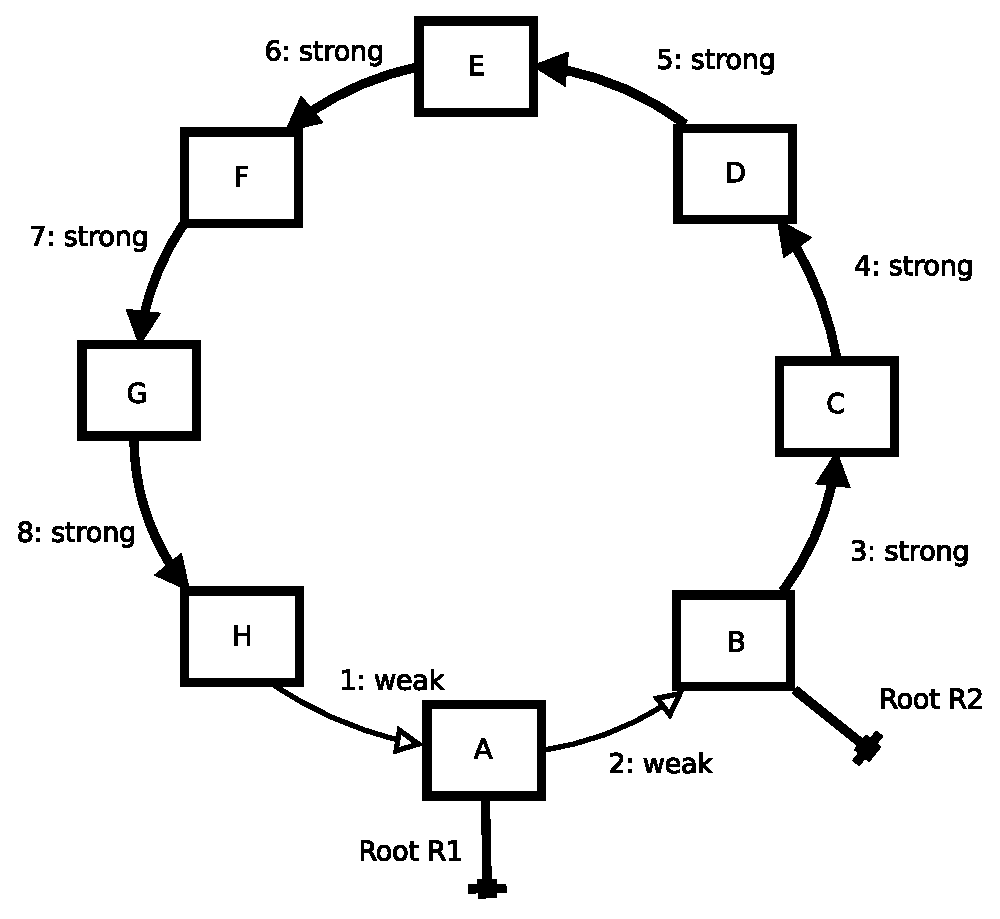
\includegraphics[width=0.32\textwidth]{figs/simplecyclenew}
\caption{When root R1 is removed, the garbage collection algorithm
only needs to trace link 2 to prove that object A does not need
to be collected.}
\label{prove}
\end{figure}

The contribution of this paper is threefold. Our algorithm never prematurely deletes any reachable object, operates in linear in time regardless of the structure (any
deletion of edges and roots takes only $\cO(N)$ time steps,
where $N$ is the number of edges in the
affected subgraph), and works concurrently with the application, without the need for system-wide pauses, i.e. ``stopping the world.''
%\update{Gokarna: We should say something like this: Moreover, our GC algorithm guarantees that no more total work is spent in the GC than in allocation (within constant factors).
%That is, a series of addition and deletion of edges do not increase the cost of collection dramatically.
%First we need to figure what Baker proved back in 1978. either outline guarantees similar to Baker or say it does not apply }
This is in contrast to Brownbridge's original algorithm and its variants \cite{Brownbridge1985,Salkild1987,Pepels1988} which can not handle concurrency issues that arise in modern multiprocessor architectures~\cite{Roy:1998}.

Our algorithm does, however, add a third kind of pointer, a {\em phantom pointer}, which identifies a temporary state that is neither strong nor weak. The addition of the space overhead offsets the time overhead in Brownbridge's work.

%Our contribution does not consist of a production-ready nor a fully optimized collector.
%Rather, we provide a proof-of-concept implementation that emphasizes correctness and time complexity.% The
%use of strong/weak pointer types provides an avenue for reduced reference traversal which
%should be especially beneficial in a distributed setting.


\subsection{Most Related Work: Premature Collection, Non-termination, and Exponential Cleanup Time}
\label{section:exponential}
Before giving details of our algorithm in Section \ref{section:high-level} %and giving details in Section \ref{section:algorithm}
-- which in turn is a modification of Brownbridge's algorithm and its variants \cite{Brownbridge1985,Salkild1987,Pepels1988} -- we first describe the problems with previous variants. In doing so, we follow the description given in the excellent garbage collection book due to Jones and Lins \cite{Jones1996}.

It was proven by McBeth \cite{McBeth1963} in early sixties that reference counting collectors were unable to handle cyclic structures; several attempts to fix this problem appeared subsequently, e.g. \cite{Friedman1979,Bobrow1980,Lins2008}. We give details in Section \ref{subsection:otherrelated}.
In contrast to the approach followed in \cite{Friedman1979,Bobrow1980,Lins2008} and several others,
Brownbridge \cite{Brownbridge1985} proposed, in 1985, a strong/weak pointer algorithm to tackle the problem of reclaiming cyclic data structures by distinguishing cycle closing pointers (weak pointers) from other references (strong pointers) \cite{Jones1996}. %different algorithm to tackle the problem of reclaiming cyclic structures using strong and weak pointers.
This algorithm relied on maintaining two invariants: (a) there are no cycles in strong pointers and (b) all items in the graph must be strongly reachable from the roots.

Some years after the publication, Salkild \cite{Salkild1987} showed that Brownbridge's algorithm
\cite{Brownbridge1985} could reclaim objects prematurely in some
configurations, e.g. a double cycle. If the last strong pointer (or link) to
an object in one cycle but not the other was lost, Brownbridge's
method would incorrectly claim nodes from the cycle.
Salkild \cite{Salkild1987} corrected this problem by proposing
that if the last strong link was removed from an object which still
had weak pointers, a collection process should re-start from that node.
While this approach eliminated the premature deletion problem, it introduced a
potential non-termination problem.

Subsequently, Pepels et al.~\cite{Pepels1988} proposed a new algorithm based on
Brownbridge-Salkild's algorithm and solved the problem of non-termination by
using a marking scheme. In their algorithm, they used two kinds of mark: one to
prevent an infinite number of searches, and the other to guarantee termination
of each search. Although correct and terminating, Pepels et al.'s algorithm is far more
complex than Brownbridge-Salkild's algorithm and in some cyclic structures the
cleanup cost complexity becomes at least
exponential in the worst-case \cite{Jones1996}. This is due to the fact that when
cycles occur, whole state space searches from
each node in the cyclic graph must be initiated, possibly many times. After Pepels et al.'s algorithm, we are not aware
of any other work on reducing the cleanup cost or complexity of the Brownbridge
algorithm. Moreover, there is no concurrent collection technique using this approach which can be applicable for the garbage collection in modern multiprocessors.

The algorithm we present in this paper removes all the limitations described above.
Our algorithm does not perform searches as such.
Instead, whenever a node
loses its last strong reference and still has weak references, it marks all
affected links as phantom. When this process is complete for
a subgraph, the system recovers the affected subgraph by converting phantom
links to either strong or weak. Because this process is a transformation from
weak or strong to phantom, and from phantom to weak or strong, it has at most
two steps and is, therefore, manifestly linear in the number of links, i.e. it
has a complexity of only $\cO(N)$ time steps,
where $N$ is the number of edges in the
affected subgraph. Moreover, in contrast to Brownbridge's algorithm, our algorithm is concurrent and is suitable for multiprocessors.

\subsection{Other Related Work}
\label{subsection:otherrelated}
Garbage collection is
an automatic memory management technique which is considered to be an important tool for developing fast as well as reliable software.  Garbage collection has been studied extensively in computer science for more than five decades, e.g., \cite{McBeth1963,Brownbridge1985,Salkild1987,Pepels1988,Bacon2001,Bacon:2001:JWC,Barabash2005,Jones1996}. %,Wilson1992}. %We refer readers to these books \cite{Jones1996,Jones2011} and these surveys \cite{Chase1987,Wilson1992} for the overview of the research in this field.
Reference counting is a widely-used form of garbage collection whereby each object has a count of the number of references to it; garbage is identified by having a reference count of zero \cite{Bacon2001}.
Reference counting approaches were first developed for LISP by Collins \cite{Collins1960}.
% in the context of a process suspension problem in LISP \cite{McCarthy1960}.
%Improvements to the initial algorithms were proposed in several subsequent papers.
Improved variations were proposed in several subsequent papers, e.g. \cite{Friedman1979,Hughes1987,Jones1996,Lins2008,Levanoni2006}. We direct readers to Shahriyar et al.~\cite{Shahriyar:2012} for the valuable overview of the current state of reference counting collectors.

It was noticed by McBeth \cite{McBeth1963} in early sixties that reference counting collectors were unable to handle cyclic structures.
After that several reference counting collectors were developed, e.g. \cite{Friedman1979,Bobrow1980,Lins:1992:CRC,Lins:2002:EAC}.
The algorithm in Friedman \cite{Friedman1979} dealt with recovering cyclic data in immutable structures, whereas Bobrow's algorithm \cite{Bobrow1980}
can reclaim all cyclic structures but relies on the explicit
information provided by the programmer. 
Trial deletion approach was studied by Christopher \cite{Christopher1984} which tries to collect cycles by identifying groups of self-sustaining objects. 
Lins \cite{Lins:1992:CRC} used a cyclic buffer to reduce repeated scanning of the same nodes in their mark-scan algorithm for cyclic reference counting. Moreover, in \cite{Lins:2002:EAC}, Lins improved his algorithm  from \cite{Lins:1992:CRC} by eliminating the scan operation through the use of a Jump-stack data structure.
%Reference counting garbage collectors developed recently were augmented with either a tracing collector or a cycle detector to reclaim cyclic structures, e.g. \cite{Bacon2001,Paz2007,Lins2008}.
%We refer the reader to \cite{Abdullahi1998,Jones2011} for details.
%For example, the reference counting collector proposed in \cite{Paz2007} combines the sliding view collector of \cite{Levanoni2006} with the cycle collector of \cite{Bacon2001}.


%Friedman and Wise's algorithm \cite{Friedman1979} was specialized to recovering cyclic data in immutable structures. Bobrow's algorithm \cite{Bobrow1980}
%can reclaim all cyclic structures but relies on the explicit
%information provided by the programmer. Hughes\cite{Hughes1987}, in his unpublished note, improved Bobrow's algorithm by avoiding the need of the extra information provided by the programmer.
%The details of other subsequent work is this area can be found in \cite{Chase1987,Wilson1992,Jones1996,Jones2011,Lins2006,Lins2008,Levanoni2006,Axford1990}.

% and some recent work on cyclic reference counting is in \cite{Lins2006,Lins2008,,Levanoni2006}.

%In 1985, Brownbridge \cite{Brownbridge1985} proposed a different algorithm to tackle the problem of reclaiming cyclic structures using strong and weak pointers. This algorithm was relied on maintaining two invariants: (a) there are no cycles in strong pointers and (b) all items in the graph must be strongly reachable from the root node. Unfortunately, his algorithm was shown incorrect by  Salkild \cite{Salkild1987}. Salkild observed that Brownbridge's algorithm sometimes reclaims objects prematurely and gave a new algorithm that corrected Brownbridge's algorithm in \cite{Salkild1987}. However, this algorithm suffers from non-termination in certain situations due to the fact that it may need infinite number of searches to determine the garbage cells. Pepels et al.~\cite{Pepels1988} proposed a new algorithm based on Brownbridge-Salkild's
%algorithm and solved the problem of non-termination by using a marking scheme. In their algorithm, they used two kinds of mark: one to prevent an infinite number of searches, and the other to guarantee termination of each search. Although correct and terminating, the algorithm is far more complex than  Brownbridge-Salkild's algorithm and in some cyclic structures the cleanup cost complexity of Pepel et al.'s algorithm becomes exponential in the worst-case \cite{Jones1996}.
%After Pepel et al.'s algorithm, we are not aware of any other work on making the cleanup cost complexity of Brownbridge's algorithm linear.
%The algorithm we present in this paper removes all the limitations of original Brownbridge's algorithm \cite{Brownbridge1985} and also its variants \cite{Salkild1987,Pepels1988} and provides linear number of searches, guarantees termination, and limits the cleanup cost complexity to $\cO(N)$, in the worst-case, where $N$ is the number of cells in a cycle.

%mark-sweep \cite{Cohen1967}.

%\input{distributed_refs}

% Note: Gokarna had a lot of this backwards. He was contrasting reference counting
% to stop-the-world collectors, and the kinds of write barriers he was concerned with
% are present in our system.
With the advancement of multiprocessor architectures,
reference counting garbage collectors have become popular because
they do not require all application threads to be stopped before the garbage collection algorithm can run~\cite{Levanoni2006}.
Recent work in reference counting algorithms, e.g. \cite{Barabash2005,Levanoni2006,Bacon2001,Bacon:2001:JWC}, try to
reduce concurrent operations and increase the efficiency of reference counting collectors.
Since our collector is a reference counting collector, it can potentially benefit from the
same types of optimizations discussed here. We leave that, however, to a future work.

%In contrast to simple stop-the-world garbage collectors which completely halt execution of the application to run a collection cycle, concurrent garbage collectors (and also incremental garbage collectors, e.g. \cite{Barabash2005}) interleave the collection cycles with the application to reduce the
%disruption of the stop-the-world approach.
%However, reference counting based garbage collectors have an inherence limitation with respect to concurrency in multiprocessor architectures in the sense that the update of the reference
%counts must be atomic since they are being updated by all
%application threads, and, when updating a pointer,
%a thread must know the previous value of the pointer-slot
%being updated despite many parallel writes from concurrent application threads \cite{Levanoni2006}.
%
%remove the requirement of atomic and synchronization operations for updating pointers and reference counts while running them on multiprocessors and also
%
%% Therefore,
%in order to make better use of the processing capacity and the parallelism  available in multiprocessors, reference counting based concurrent
%collectors have been presented and studied, e.g. \cite{Barabash2005,Levanoni2006,Bacon2001,Bacon:2001:JWC}. % garbage collection is also considered for several other particular systems, namely concurrent systems, real-time systems, mobile actor systems, and asynchronous distributed systems \cite{Pizlo2008,Huelsbergen1998,Wang2006,Wang2010,Kafura1995,Veiga2005}. Pizlo et al. \cite{Pizlo2008} studied concurrent real-time garbage collectors.
%However, reference counting based garbage collectors have an inherence limitation with respect to concurrency in multiprocessor architectures in the sense that the update of the reference
%counts must be atomic since they are being updated by all
%application threads, and, when updating a pointer,
%a thread must know the previous value of the pointer-slot
%being updated despite many parallel writes from concurrent application threads \cite{Levanoni2006}.
%Therefore, these papers \cite{Barabash2005,Levanoni2006,Bacon2001,Bacon:2001:JWC} shed light on how to obtain better algorithms by focusing thoroughly on reducing synchronization requirements and improving throughput and latency.

However, as mentioned earlier, reference counting garbage collectors cannot collect cycles \cite{McBeth1963}. Therefore, concurrent reference counting collectors \cite{Barabash2005,Levanoni2006,Bacon2001,Bacon:2001:JWC,Paz2007,Lins2008} use other techniques, e.g. they supplement the reference counter with a tracing collector or a cycle detector, together with their concurrent reference counting algorithm. For example, the reference counting collector proposed in \cite{Paz2007} combines the sliding view reference counting concurrent collector of \cite{Levanoni2006} with the cycle collector of \cite{Bacon2001}. Our collector has some similarity with these, in that our $Phantomization$ process may traverse many nodes. It should, however, trace fewer nodes and do so less frequently. Recently, Frampton provides a detailed study of cycle collection in his PhD thesis \cite{Frampton2010}.
%To the best of our knowledge, we are not aware of any existing reference counting algorithm that itself can reclaim cycles.
%\todo{Steve: is it OK to say this statement}
%We note here that it is challenging to develop a variation of referencing counting collectors which collect cycles without the need of an auxiliary collector dedicated for reclaiming cycles. Our algorithm is a significant step towards this direction. xxx

%a backup tracing collector or a cycle detector to reclaim cyclic structures \cite{Bacon2001,Paz2007,Lins2008}.

%Otherwise, a confusion occurs in the bookkeeping of
%the reference counts. Thus, the naive solution requires a lock
%on any update operation. More advanced solutions have recently reduced this overhead to a compare-and-swap operation, which is still a time consuming write-barrier. Recent developments lead to better algorithm \cite{Levanoni2006}\cite{Barabash2005} based on reference counting but they can not collect cycles. They used mark-and-sweep algorithm together with the reference counting algorithm \cite{Levanoni2006}.
%Bacon et al. \cite{Bacon2001,Bacon:2001:JWC} also studied on-the-fly reference counting algorithms for multiprocessors. These all work focused on reducing synchronization and improving throughput and latency. They did not elaborate further on how to avoid the limitations of reference counting algorithms in reclaiming cycles.
%Huelsbergen and Winterbottom \cite{Huelsbergen1998} extended the mark-and-sweep garbage collection technique to a concurrent setting.
%A parallel, incremental, mostly concurrent garbage collector for servers is given in \cite{Barabash2005}.

%Recently, garbage collection is also considered for several other particular systems, namely concurrent systems, real-time systems, mobile actor systems, and asynchronous distributed systems \cite{Pizlo2008,Huelsbergen1998,Wang2006,Wang2010,Kafura1995,Veiga2005}. Pizlo et al. \cite{Pizlo2008} studied concurrent real-time garbage collectors.
%Huelsbergen and Winterbottom \cite{Huelsbergen1998} extended the mark-and-sweep garbage collection technique to a concurrent setting.
%A parallel, incremental, mostly concurrent garbage collector for servers is given in \cite{Barabash2005}.
%%Distributed garbage collection for mobile actor systems is studied in several papers, e.g. \cite{Wang2006,Wang2010}, using the pseudo root approach and also through vertex-preserving actor-to-object graph transformations.
%%Veiga and Ferreira \cite{Veiga2005} presented a garbage collection technique for asynchronous distributed systems.
%%Kafura et al. \cite{Kafura1995} presented a distributed and concurrent garbage collection algorithm for active objects. Their algorithm is snapshot based.



Herein we have tried to cover a sampling of garbage collectors that are most relevant to our work.

Apple's ARC memory management system makes a distinction between ``strong'' and ``weak'' pointers, similar to what we describe here. In the ARC memory system, however, the type of each pointer must be specifically designated by the programmer, and this type will not change during the program's execution. If the programmer gets the type wrong, it is possible for ARC to have strong cycles as well as prematurely deleted objects. With our system, the pointer type is automatic and can change during the execution. Our system protects against these possibilities, at the cost of lower efficiency.

There exist other concurrent techniques optimized for both uniprocessors as well as multiprocessors. Generational concurrent garbage collectors were also studied, e.g. \cite{Printezis:2000}. Huelsbergen and Winterbottom \cite{Huelsbergen1998} proposed an incremental algorithm for the concurrent garbage collection that is a variant of mark-and-sweep collection scheme first proposed in \cite{McCarthy1960}.
%Recently, McGachey et al. \cite{McGachey2008} considered how to build a concurrent garbage collector from a state of the art software transactional memory system \cite{Shavit1997}. 
Furthermore, garbage collection is also considered for several other systems, namely real-time systems %, mobile actor systems, 
and asynchronous distributed systems, e.g. \cite{Pizlo2008,Veiga2005}. %Wang2010,Huelsbergen1998,Kafura1995,
%However, we do not explore this area in this present work, but we conjecture that our technique can be useful to these systems and deserves further work (some possible directions are outlined in Section \ref{section:future-work}).

%Brownbridge's algorithm \cite{Brownbridge1985}, and its subsequent improvements due to Salkild\cite{Salkild1987}, and Pepels et al. \cite{Pepels1988}, which we describe later in Section \ref{section:exponential}.

Concurrent collectors are gaining popularity. The concurrent collector described in Bacon and Rajan~\cite{Bacon2001} can be considered to be one of the more efficient reference counting concurrent collectors. The algorithm uses two counters per object, one for the actual reference count and other for the cyclic reference count. Apart from the number of the counters used, the cycle detection strategy requires a minimum of two traversals of cycle when the cycle is reachable and eleven cycle traversals when the cycle is garbage.
%The necessity of eleven traversals of cyclic objects for safety conditions and difficulty in making the algorithm parallel easily began as the motivation of the work. So our work concentrates on the concurrency as well as parallel aspect of the collectors along with amortizing the number of the traversal required in the cycle detection strategies. Our approach uses two traversals for the deletion of the cycle and needs two traversal of the affected graph when the object is speculated wrongly as cycle. So we give tight upper bound on the number of the traversal happens in the affected graph for every event in the graph.

%\todo{Hari, say something more about \cite{Bacon2003,Bacon2001,Bacon:2001:JWC}}


\subsection{Paper Organization}
The rest of the paper is organized as follows. We present %the high level overview of
our strong/weak/phantom pointer based concurrent garbage collector in Section~\ref{section:high-level} with some examples. %We then give the details of the collector in Section~\ref{section:algorithm}.
In Section~\ref{section:correctness}, we sketch proofs of its correctness and complexity properties. In Section~\ref{section:experimental}, we give some experimental results. We conclude the paper with future research directions in Section~\ref{section:future-work} and a short discussion in Section~\ref{section:conclusion}. Detailed algorithms may be found in the appendix.
% The source code of our concurrent collector implementation can be found in~\cite{url:refimpl}.

%\subsection{Other Related Work}
\label{subsection:otherrelated}
Garbage collection is
an automatic memory management technique which is considered to be an important tool for developing fast as well as reliable software.  Garbage collection has been studied extensively in computer science for more than five decades, e.g., \cite{McBeth1963,Brownbridge1985,Salkild1987,Pepels1988,Bacon2001,Bacon:2001:JWC,Barabash2005,Jones1996}. %,Wilson1992}. %We refer readers to these books \cite{Jones1996,Jones2011} and these surveys \cite{Chase1987,Wilson1992} for the overview of the research in this field.
Reference counting is a widely-used form of garbage collection whereby each object has a count of the number of references to it; garbage is identified by having a reference count of zero \cite{Bacon2001}.
Reference counting approaches were first developed for LISP by Collins \cite{Collins1960}.
% in the context of a process suspension problem in LISP \cite{McCarthy1960}.
%Improvements to the initial algorithms were proposed in several subsequent papers.
Improved variations were proposed in several subsequent papers, e.g. \cite{Friedman1979,Hughes1987,Jones1996,Lins2008,Levanoni2006}. We direct readers to Shahriyar et al.~\cite{Shahriyar:2012} for the valuable overview of the current state of reference counting collectors.

It was noticed by McBeth \cite{McBeth1963} in early sixties that reference counting collectors were unable to handle cyclic structures.
After that several reference counting collectors were developed, e.g. \cite{Friedman1979,Bobrow1980,Lins:1992:CRC,Lins:2002:EAC}.
The algorithm in Friedman \cite{Friedman1979} dealt with recovering cyclic data in immutable structures, whereas Bobrow's algorithm \cite{Bobrow1980}
can reclaim all cyclic structures but relies on the explicit
information provided by the programmer. 
Trial deletion approach was studied by Christopher \cite{Christopher1984} which tries to collect cycles by identifying groups of self-sustaining objects. 
Lins \cite{Lins:1992:CRC} used a cyclic buffer to reduce repeated scanning of the same nodes in their mark-scan algorithm for cyclic reference counting. Moreover, in \cite{Lins:2002:EAC}, Lins improved his algorithm  from \cite{Lins:1992:CRC} by eliminating the scan operation through the use of a Jump-stack data structure.
%Reference counting garbage collectors developed recently were augmented with either a tracing collector or a cycle detector to reclaim cyclic structures, e.g. \cite{Bacon2001,Paz2007,Lins2008}.
%We refer the reader to \cite{Abdullahi1998,Jones2011} for details.
%For example, the reference counting collector proposed in \cite{Paz2007} combines the sliding view collector of \cite{Levanoni2006} with the cycle collector of \cite{Bacon2001}.


%Friedman and Wise's algorithm \cite{Friedman1979} was specialized to recovering cyclic data in immutable structures. Bobrow's algorithm \cite{Bobrow1980}
%can reclaim all cyclic structures but relies on the explicit
%information provided by the programmer. Hughes\cite{Hughes1987}, in his unpublished note, improved Bobrow's algorithm by avoiding the need of the extra information provided by the programmer.
%The details of other subsequent work is this area can be found in \cite{Chase1987,Wilson1992,Jones1996,Jones2011,Lins2006,Lins2008,Levanoni2006,Axford1990}.

% and some recent work on cyclic reference counting is in \cite{Lins2006,Lins2008,,Levanoni2006}.

%In 1985, Brownbridge \cite{Brownbridge1985} proposed a different algorithm to tackle the problem of reclaiming cyclic structures using strong and weak pointers. This algorithm was relied on maintaining two invariants: (a) there are no cycles in strong pointers and (b) all items in the graph must be strongly reachable from the root node. Unfortunately, his algorithm was shown incorrect by  Salkild \cite{Salkild1987}. Salkild observed that Brownbridge's algorithm sometimes reclaims objects prematurely and gave a new algorithm that corrected Brownbridge's algorithm in \cite{Salkild1987}. However, this algorithm suffers from non-termination in certain situations due to the fact that it may need infinite number of searches to determine the garbage cells. Pepels et al.~\cite{Pepels1988} proposed a new algorithm based on Brownbridge-Salkild's
%algorithm and solved the problem of non-termination by using a marking scheme. In their algorithm, they used two kinds of mark: one to prevent an infinite number of searches, and the other to guarantee termination of each search. Although correct and terminating, the algorithm is far more complex than  Brownbridge-Salkild's algorithm and in some cyclic structures the cleanup cost complexity of Pepel et al.'s algorithm becomes exponential in the worst-case \cite{Jones1996}.
%After Pepel et al.'s algorithm, we are not aware of any other work on making the cleanup cost complexity of Brownbridge's algorithm linear.
%The algorithm we present in this paper removes all the limitations of original Brownbridge's algorithm \cite{Brownbridge1985} and also its variants \cite{Salkild1987,Pepels1988} and provides linear number of searches, guarantees termination, and limits the cleanup cost complexity to $\cO(N)$, in the worst-case, where $N$ is the number of cells in a cycle.

%mark-sweep \cite{Cohen1967}.

%\input{distributed_refs}

% Note: Gokarna had a lot of this backwards. He was contrasting reference counting
% to stop-the-world collectors, and the kinds of write barriers he was concerned with
% are present in our system.
With the advancement of multiprocessor architectures,
reference counting garbage collectors have become popular because
they do not require all application threads to be stopped before the garbage collection algorithm can run~\cite{Levanoni2006}.
Recent work in reference counting algorithms, e.g. \cite{Barabash2005,Levanoni2006,Bacon2001,Bacon:2001:JWC}, try to
reduce concurrent operations and increase the efficiency of reference counting collectors.
Since our collector is a reference counting collector, it can potentially benefit from the
same types of optimizations discussed here. We leave that, however, to a future work.

%In contrast to simple stop-the-world garbage collectors which completely halt execution of the application to run a collection cycle, concurrent garbage collectors (and also incremental garbage collectors, e.g. \cite{Barabash2005}) interleave the collection cycles with the application to reduce the
%disruption of the stop-the-world approach.
%However, reference counting based garbage collectors have an inherence limitation with respect to concurrency in multiprocessor architectures in the sense that the update of the reference
%counts must be atomic since they are being updated by all
%application threads, and, when updating a pointer,
%a thread must know the previous value of the pointer-slot
%being updated despite many parallel writes from concurrent application threads \cite{Levanoni2006}.
%
%remove the requirement of atomic and synchronization operations for updating pointers and reference counts while running them on multiprocessors and also
%
%% Therefore,
%in order to make better use of the processing capacity and the parallelism  available in multiprocessors, reference counting based concurrent
%collectors have been presented and studied, e.g. \cite{Barabash2005,Levanoni2006,Bacon2001,Bacon:2001:JWC}. % garbage collection is also considered for several other particular systems, namely concurrent systems, real-time systems, mobile actor systems, and asynchronous distributed systems \cite{Pizlo2008,Huelsbergen1998,Wang2006,Wang2010,Kafura1995,Veiga2005}. Pizlo et al. \cite{Pizlo2008} studied concurrent real-time garbage collectors.
%However, reference counting based garbage collectors have an inherence limitation with respect to concurrency in multiprocessor architectures in the sense that the update of the reference
%counts must be atomic since they are being updated by all
%application threads, and, when updating a pointer,
%a thread must know the previous value of the pointer-slot
%being updated despite many parallel writes from concurrent application threads \cite{Levanoni2006}.
%Therefore, these papers \cite{Barabash2005,Levanoni2006,Bacon2001,Bacon:2001:JWC} shed light on how to obtain better algorithms by focusing thoroughly on reducing synchronization requirements and improving throughput and latency.

However, as mentioned earlier, reference counting garbage collectors cannot collect cycles \cite{McBeth1963}. Therefore, concurrent reference counting collectors \cite{Barabash2005,Levanoni2006,Bacon2001,Bacon:2001:JWC,Paz2007,Lins2008} use other techniques, e.g. they supplement the reference counter with a tracing collector or a cycle detector, together with their concurrent reference counting algorithm. For example, the reference counting collector proposed in \cite{Paz2007} combines the sliding view reference counting concurrent collector of \cite{Levanoni2006} with the cycle collector of \cite{Bacon2001}. Our collector has some similarity with these, in that our $Phantomization$ process may traverse many nodes. It should, however, trace fewer nodes and do so less frequently. Recently, Frampton provides a detailed study of cycle collection in his PhD thesis \cite{Frampton2010}.
%To the best of our knowledge, we are not aware of any existing reference counting algorithm that itself can reclaim cycles.
%\todo{Steve: is it OK to say this statement}
%We note here that it is challenging to develop a variation of referencing counting collectors which collect cycles without the need of an auxiliary collector dedicated for reclaiming cycles. Our algorithm is a significant step towards this direction. xxx

%a backup tracing collector or a cycle detector to reclaim cyclic structures \cite{Bacon2001,Paz2007,Lins2008}.

%Otherwise, a confusion occurs in the bookkeeping of
%the reference counts. Thus, the naive solution requires a lock
%on any update operation. More advanced solutions have recently reduced this overhead to a compare-and-swap operation, which is still a time consuming write-barrier. Recent developments lead to better algorithm \cite{Levanoni2006}\cite{Barabash2005} based on reference counting but they can not collect cycles. They used mark-and-sweep algorithm together with the reference counting algorithm \cite{Levanoni2006}.
%Bacon et al. \cite{Bacon2001,Bacon:2001:JWC} also studied on-the-fly reference counting algorithms for multiprocessors. These all work focused on reducing synchronization and improving throughput and latency. They did not elaborate further on how to avoid the limitations of reference counting algorithms in reclaiming cycles.
%Huelsbergen and Winterbottom \cite{Huelsbergen1998} extended the mark-and-sweep garbage collection technique to a concurrent setting.
%A parallel, incremental, mostly concurrent garbage collector for servers is given in \cite{Barabash2005}.

%Recently, garbage collection is also considered for several other particular systems, namely concurrent systems, real-time systems, mobile actor systems, and asynchronous distributed systems \cite{Pizlo2008,Huelsbergen1998,Wang2006,Wang2010,Kafura1995,Veiga2005}. Pizlo et al. \cite{Pizlo2008} studied concurrent real-time garbage collectors.
%Huelsbergen and Winterbottom \cite{Huelsbergen1998} extended the mark-and-sweep garbage collection technique to a concurrent setting.
%A parallel, incremental, mostly concurrent garbage collector for servers is given in \cite{Barabash2005}.
%%Distributed garbage collection for mobile actor systems is studied in several papers, e.g. \cite{Wang2006,Wang2010}, using the pseudo root approach and also through vertex-preserving actor-to-object graph transformations.
%%Veiga and Ferreira \cite{Veiga2005} presented a garbage collection technique for asynchronous distributed systems.
%%Kafura et al. \cite{Kafura1995} presented a distributed and concurrent garbage collection algorithm for active objects. Their algorithm is snapshot based.



Herein we have tried to cover a sampling of garbage collectors that are most relevant to our work.

Apple's ARC memory management system makes a distinction between ``strong'' and ``weak'' pointers, similar to what we describe here. In the ARC memory system, however, the type of each pointer must be specifically designated by the programmer, and this type will not change during the program's execution. If the programmer gets the type wrong, it is possible for ARC to have strong cycles as well as prematurely deleted objects. With our system, the pointer type is automatic and can change during the execution. Our system protects against these possibilities, at the cost of lower efficiency.

There exist other concurrent techniques optimized for both uniprocessors as well as multiprocessors. Generational concurrent garbage collectors were also studied, e.g. \cite{Printezis:2000}. Huelsbergen and Winterbottom \cite{Huelsbergen1998} proposed an incremental algorithm for the concurrent garbage collection that is a variant of mark-and-sweep collection scheme first proposed in \cite{McCarthy1960}.
%Recently, McGachey et al. \cite{McGachey2008} considered how to build a concurrent garbage collector from a state of the art software transactional memory system \cite{Shavit1997}. 
Furthermore, garbage collection is also considered for several other systems, namely real-time systems %, mobile actor systems, 
and asynchronous distributed systems, e.g. \cite{Pizlo2008,Veiga2005}. %Wang2010,Huelsbergen1998,Kafura1995,
%However, we do not explore this area in this present work, but we conjecture that our technique can be useful to these systems and deserves further work (some possible directions are outlined in Section \ref{section:future-work}).

%Brownbridge's algorithm \cite{Brownbridge1985}, and its subsequent improvements due to Salkild\cite{Salkild1987}, and Pepels et al. \cite{Pepels1988}, which we describe later in Section \ref{section:exponential}.

Concurrent collectors are gaining popularity. The concurrent collector described in Bacon and Rajan~\cite{Bacon2001} can be considered to be one of the more efficient reference counting concurrent collectors. The algorithm uses two counters per object, one for the actual reference count and other for the cyclic reference count. Apart from the number of the counters used, the cycle detection strategy requires a minimum of two traversals of cycle when the cycle is reachable and eleven cycle traversals when the cycle is garbage.
%The necessity of eleven traversals of cyclic objects for safety conditions and difficulty in making the algorithm parallel easily began as the motivation of the work. So our work concentrates on the concurrency as well as parallel aspect of the collectors along with amortizing the number of the traversal required in the cycle detection strategies. Our approach uses two traversals for the deletion of the cycle and needs two traversal of the affected graph when the object is speculated wrongly as cycle. So we give tight upper bound on the number of the traversal happens in the affected graph for every event in the graph.

%\todo{Hari, say something more about \cite{Bacon2003,Bacon2001,Bacon:2001:JWC}}

%
%\section{Previous Approaches: Non-termination and Exponential Cleanup Time}
%\label{section:exponential}
%Before introducing our algorithm -- which in turn is a modification of Brownbridge's algorithm and its variants \cite{Brownbridge1985,Salkild1987,Pepels1988} -- we first describe the Brownbridge variants and the problems of these approaches. We follow the description given in the excellent garbage collection book due to Jones and Lins \cite{Jones1996}.
%
%In 1985, Brownbridge \cite{Brownbridge1985} proposed a weak-pointer algorithm to tackle the problem of reclaiming cyclic data structures by distinguishing cycle closing pointers (weak pointers) from other references (strong pointers) \cite{Jones1996}. %different algorithm to tackle the problem of reclaiming cyclic structures using strong and weak pointers.
%This algorithm relied on maintaining two invariants: (a) there are no cycles in strong pointers and (b) all items in the graph must be strongly reachable from the root node.
%
%Salkild \cite{Salkild1987} showed that Brownbridge's algorithm
%\cite{Brownbridge1985} could reclaim objects prematurely in some
%configurations, e.g. a double cycle. If the last strong link to
%an object in one cycle but not the other was lost, Brownbridge's
%method would incorrectly claim nodes from the cycle.
%
%Salkild \cite{Salkild1987} corrected this problem by proposing
%that if the last strong link was removed from an object which still
%had weak pointers, a collection process should re-start from that node.
%While this eliminated the premature deletion problem, it introduced a
%potential non-termination problem.
%
%Pepels et al.~\cite{Pepels1988} proposed a new algorithm based on
%Brownbridge-Salkild's algorithm and solved the problem of non-termination by
%using a marking scheme. In their algorithm, they used two kinds of mark: one to
%prevent an infinite number of searches, and the other to guarantee termination
%of each search. Although correct and terminating, the algorithm is far more
%complex than Brownbridge-Salkild's algorithm and in some cyclic structures the
%cleanup cost complexity of Pepels et al.'s algorithm becomes at least
%exponential in the worst-case \cite{Jones1996}. This is due to the fact that in
%cyclic situations, this algorithm needs to perform whole state space search from
%each node in the cyclic graph. After Pepels et al.'s algorithm, we are not aware
%of any other work on reducing the cleanup cost or complexity of the Brownbridge
%algorithm.
%
%The algorithm we present in this paper removes all the limitations described
%above. Our algorithm does not perform searches, as such. Instead, whenever a node
%loses its last strong reference and still has weak references, it marks all
%affected links as phantom. When this process is complete for
%a subgraph, the system recovers the affected subgraph by converting phantom
%links to either strong or weak. Because this process is a transformation from
%weak or strong to phantom, and from phantom to weak or strong, it has at most
%two steps and is, therefore, manifestly linear in the number of links, i.e. it
%has a complexity of $\cO(N)$, where $N$ is the number of links in a subgraph.

\section{Algorithm}
\label{section:high-level}
In this section, we present our concurrent garbage collection algorithm.
%The pseudocode description of our collector is given in Algorithms \ref{algorithm:linkset}--\ref{algorithm:cleanup}.
Each object in the heap contains three reference counts: the first
two are the strong and weak, the third is the phantom count. Each object also
contains a bit named {\tt which} (Brownbridge \cite{Brownbridge1985} called it the ``strength-bit'')
to identify which of the first two counters is
used to keep track of strong references, as well as a boolean called {\tt
phantomized} to keep track of whether the node is phantomized.
Outgoing links (i.e., pointers) to other objects must also contain (1) a {\tt which} bit to
identify which reference counter on the target object they increment, and (2) a {\tt
phantom} boolean to identify whether they have been phantomized. This data structure for each object can be seen in the example given in Fig.~\ref{ex1}.

%Local creation of links only allows the creation of strong references when no
%cycle creation is possible. This includes links from (i) all root
%references i.e. references from the stack or global space; (ii) all links made from
%objects who have no strong links from other objects, i.e. objects whose only strong
%links are from roots; (iii) all links made to objects with no
%outgoing links, i.e. right after object creation and before outgoing references are
%initialized; and (iv) all objects whose outgoing links are phantomized. All
%self-references are weak. Any other link is created weak. See Algorithm~\ref{algorithm:linkset}.

Local creation of links only allows the creation of strong references when no
cycle creation is possible. Consider the creation of a link from a source object $S$
to a target object $T$. The link will be created strong if (i) the only strong
links to $S$ are from roots i.e. there is no object $C$ with a strong link to $S$;
(ii) object $T$ has no outgoing links i.e. it is newly created and its outgoing links are
not initialized; and (iii) object $T$ is phantomized, and $S$ is not. All
self-references are weak. Any other link is created phantom or weak.
%See Algorithm~\ref{algorithm:linkset}.

To create a strong link, the {\tt which} bit on the link must match the value of
the {\tt which} bit on the target object. A weak link is created by setting the
{\tt which} bit on the reference to the complement of the value of the {\tt
which} bit on the target.

When the strong reference count on any object reaches zero, the garbage
collection process begins.
If the object's weak reference count is zero, the
object is immediately reclaimed. If the weak count is positive, then a
a sequence of three phases is initiated: $Phantomization$, $Recovery$, and $CleanUp$.
In $Phantomization$, the object toggles its {\tt which} bit, turning its
incoming weak reference counts to strong ones,
and phantomizes its outgoing links.
%See Algorithm~\ref{algorithm:linkfree}.

Phantomizing a link transfers a reference count (either strong or weak), to the
phantom count on the target object. If this causes the object to lose its
last strong reference, then the object may also phantomize, i.e. toggle its {\tt which} bit (if that
will cause it to gain strong references), %see Algorithm~\ref{algorithm:phantomizenode}),
and phantomizes all its outgoing
links. This process may spread to a large number of target objects.
%See Algorithm~\ref{algorithm:phantomizelink}.

All objects touched in the process of a phantomization that were able to recover
their strong references by toggling their {\tt which} bit are remembered and put
in a ``recovery list''.
%(see Algorithm~\ref{algorithm:main}).
When phantomization is finished, $Recovery$ begins, starting with all objects in the recovery list.

To perform a recovery, the system looks at each object in the recovery list,
checking to see whether it still has a positive strong reference count. If it
does, it sets the {\tt phantomized} boolean to false, and rebuilds its outgoing
links, turning phantoms to strong or weak according to the rules above. If a
phantom link is rebuilt and the target object regains its first strong reference
as a result, the target object sets its {\tt phantomized} boolean to false and
attempts to recover its outgoing phantom links (if any). The recovery continues
to rebuild outgoing links until it terminates. %See Algorithm~\ref{algorithm:rebuild}.

Finally, after the recovery is complete, $CleanUp$ begins. The recovery list is revisited a second
time. Any objects that still have no strong references are deleted. %See Algorithm~\ref{algorithm:cleanup}.

Note that all three of these phases, $Phantomization$, $Recovery$, and $CleanUp$ are,
by their definitions, linear in the number of links; we prove this formally in Theorem \ref{theorem:termination} in Section \ref{section:correctness}. Links can undergo only one
state change in each of these phases: strong or weak to phantom during
$Phantomization$, phantom to strong or weak during $Recovery$, and phantom to
deleted in $CleanUp$. %We will describe each algorithm in detail in full version.

We now present some examples to show how our algorithm performs collection in several real word scenarios.

%\section{Algorithm}
%\label{section:algorithm}
%Each object / node
%in the graph has set of methods to be used by collector threads. Each collector
%thread reads the message from the queue and delivers the message to the object
%and perform consequences of the message. The queue works in phases. All the
%messages enqueued in the queue belongs to the three phases of the queue. They
%are Phantomization, Restoration and CleanUp. So the queue is aligned based on
%the circular priority. They round-robin the priority of the queue in the order
%mentioned. So everytime a collector reads a message there is no message in the
%queue that is in higher priority than one read now. Every object has a method
%associated with each kind of the message read. So collector calls the appropiate
%method on the object to process the message. We go from the each message and it
%subsequent operations. When any links are modified or deleted, the incoming link
%lost will be processed. Algorithm \ref{algorithm:incoming} explains the actions
%taken in the presence of link lost. A link lost can lead to two action one being
%the deletion when there are no more roots supporting it and other being the
%detection of cycle in the objects and deleting if necessary. The deletion
%scenario is executed when the object processed has no incoming support apart
%from the lost link. The later scenario which require the object to detect if it
%is a part of the cyclic structure, it intiates the phantomization process by
%flipping its required bits and starts collapsing the graph of nodes. The process
%collapsing is often used synonymously with phantomization. Algorithm
%\ref{algorithm:phantomization} performs the phantomization by sending phantomize
%link message to all the childrens of the node along with certain votes that the
%originating node expects to identify the completion of the phantomization
%process. These votes are returned by any phantomized node when there are no more
%node to be phantomized as their children. Precisely, the process of
%phantomization of the children is called as collapsing the structure. In the
%collapse process, each node uses the phantomization routine to phantomize all
%the kids and also identifies the potential recovery points the in the traversed
%path. The collapse is the visiting routine that marks the objects visited with
%the originator of this collapse. The collapse routine is clearly formalized in
%Algorithm \ref{algorithm:collapse}.

\subsection{Example: A Simple Cycle}

In Fig.~\ref{ex1} we see a cyclic graph with three nodes. This figure shows
the counters, bits, and boolean values in full detail to make it clear how
these values are used within the algorithm. Objects are represented with
circles, links have a pentagon with state information at their start and
an arrow at their end.

In Step 0, the cycle is supported by a root, a reference from stack or global
space. In Step 1, the root reference is removed, decrementing the strong
reference by one, and beginning a $Phantomization$. Object C toggles its which pointer and
phantomizes its outgoing links. Note that toggling the which pointer causes the
link from A to C to become strong, but nothing needs to change on A
to make this happen.

In Step 2, object B also toggles its which bit, and phantomizes its
outgoing links. Likewise, in Step 3, object A phantomizes, and the
$Phantomization$ phase completes.

$Recovery$ will attempt to unphantomize objects A, B, and C. None of them,
however, have any strong support, and so none of them recover.

$Cleanup$ happens next, and all objects are reclaimed.

%Because A has no strong
%support but does have weak support, it initiates phantomization. The node is
%marked as phantomized (using an asterisk), and incoming support becomes strong
%and outgoing support becomes a phantom. In the next step object B begins to
%phantomize, and turns its its outgoing reference to a phantom. All links are now
%phantoms and the phantomization is complete.

%\begin{figure}
%\centering
%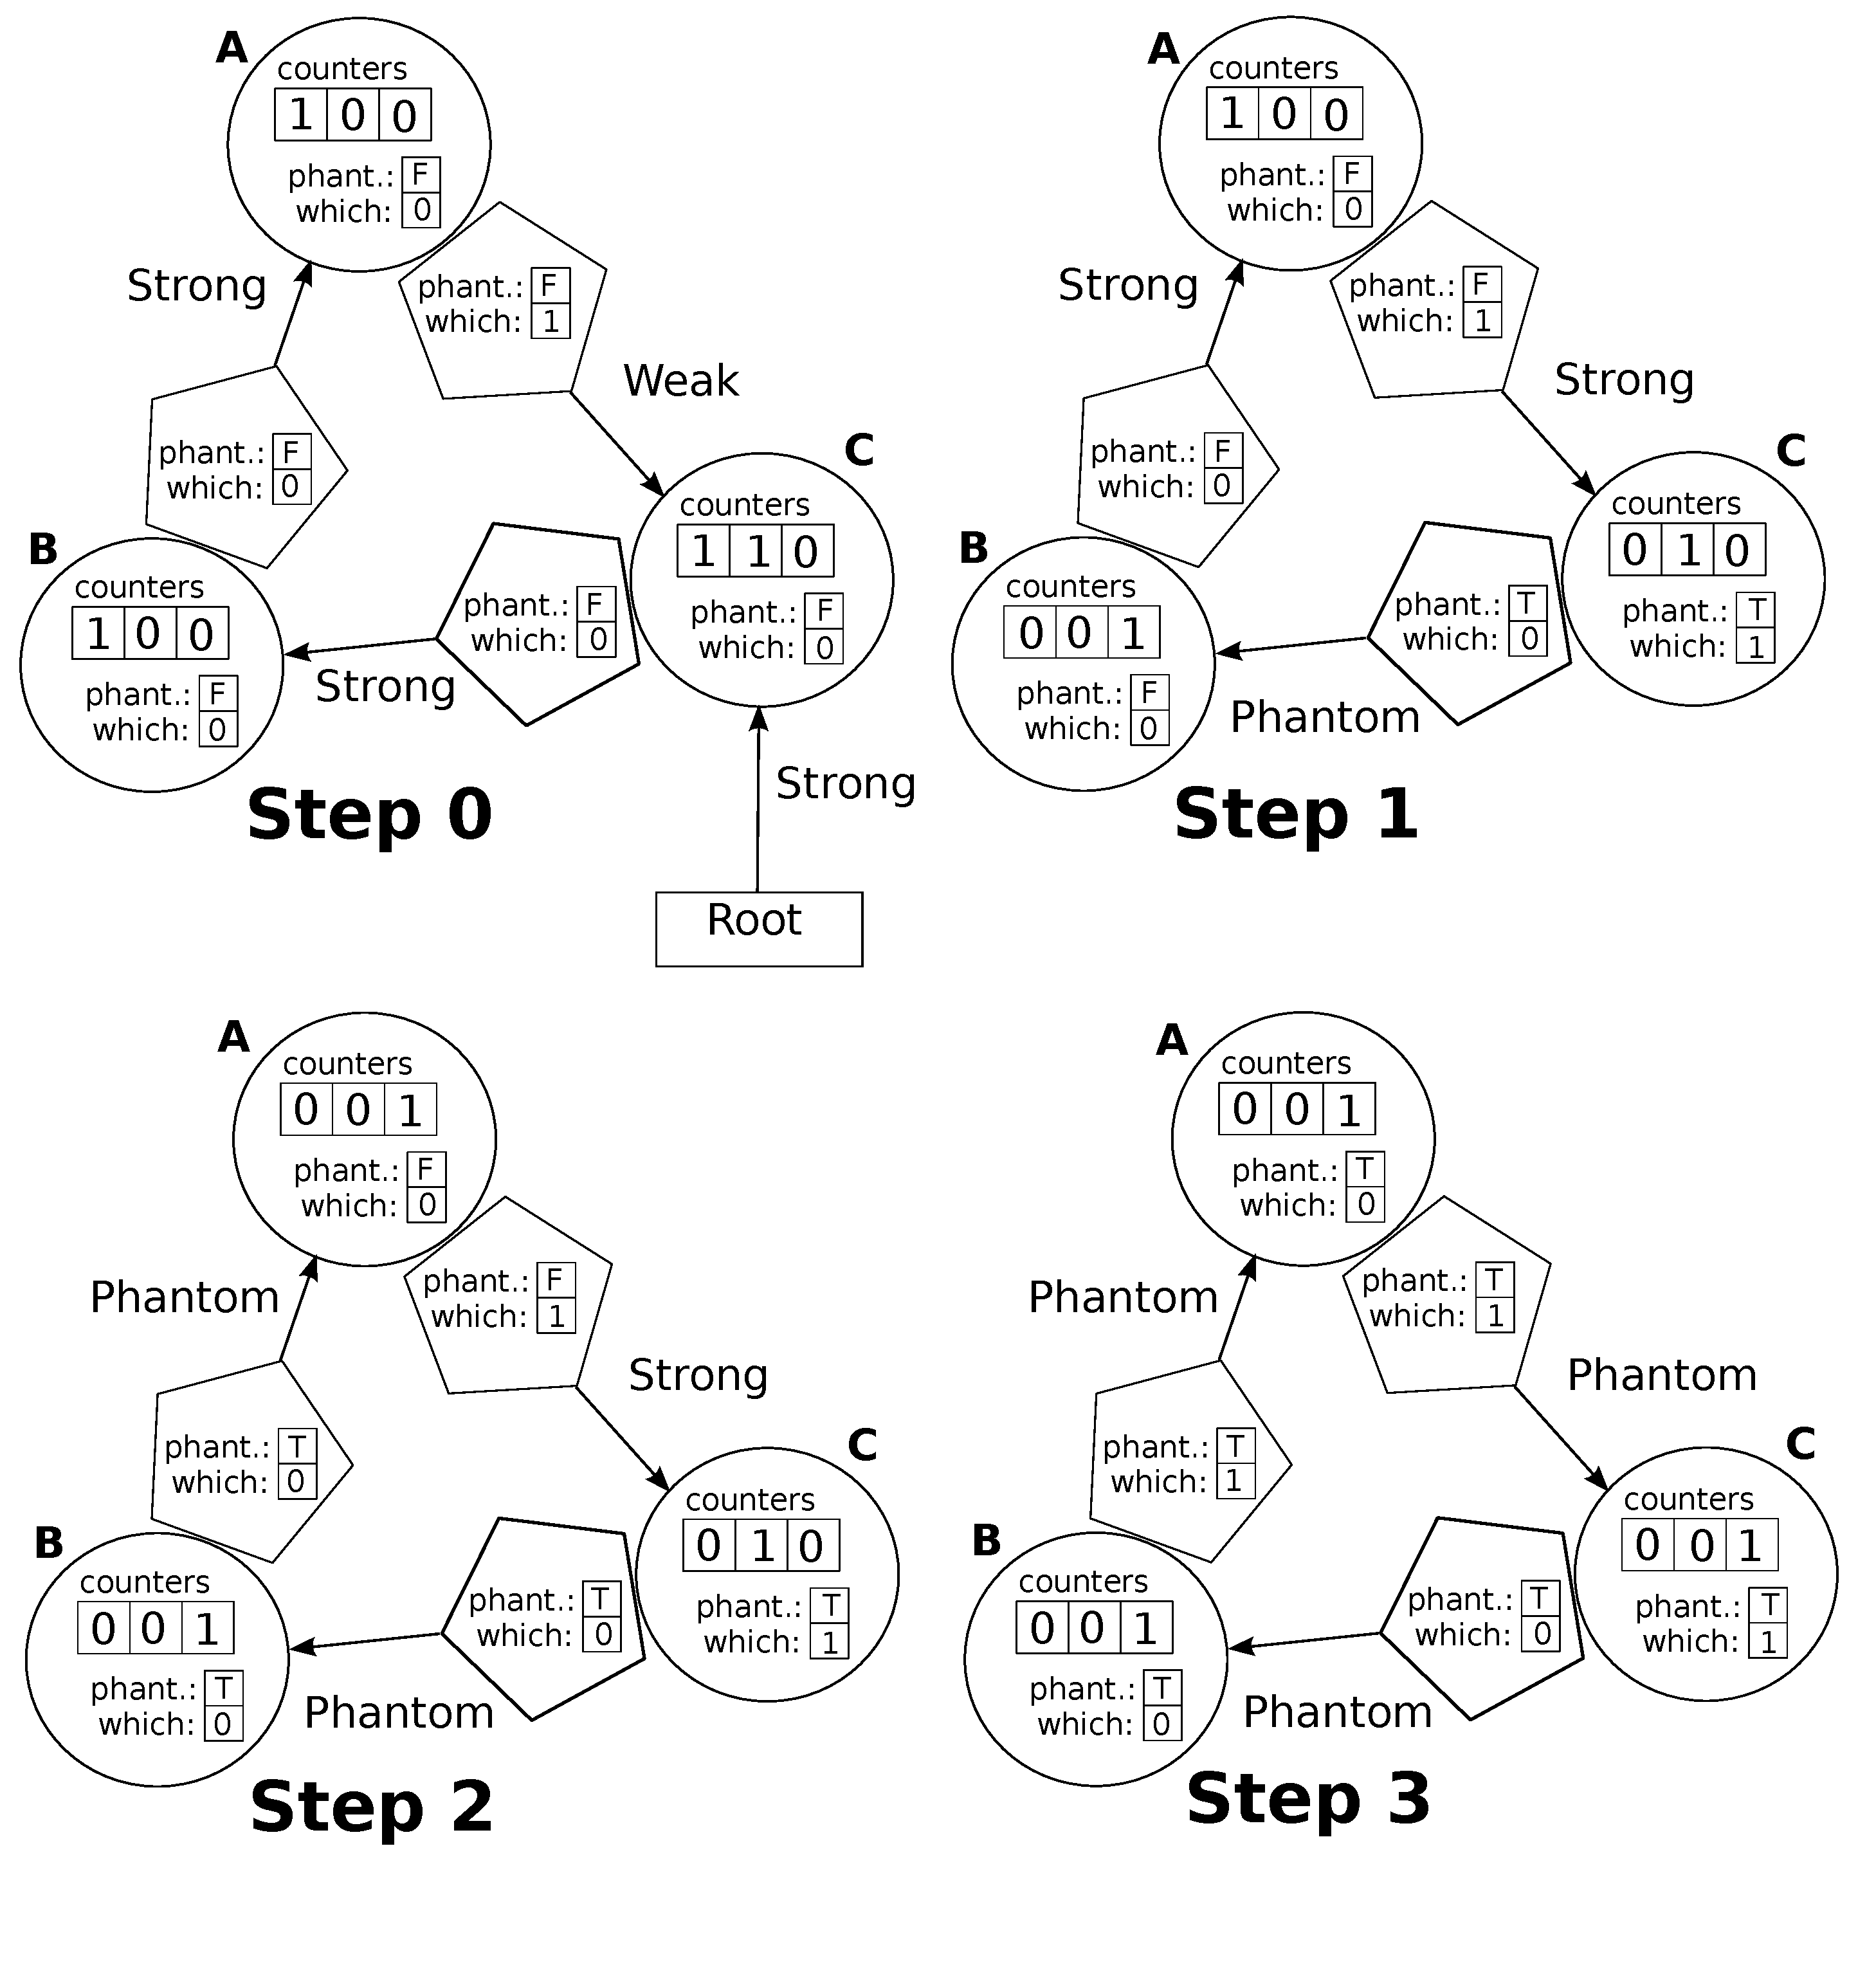
\includegraphics[width=0.5\textwidth]{figs/method}
%\caption{Reclaiming a cycle with three objects.}
%\label{ex1}
%\end{figure}

\begin{figure*}[!t]
  \centering
  %\subfloat[Initially, the owner node $v$ publishes the object]
  {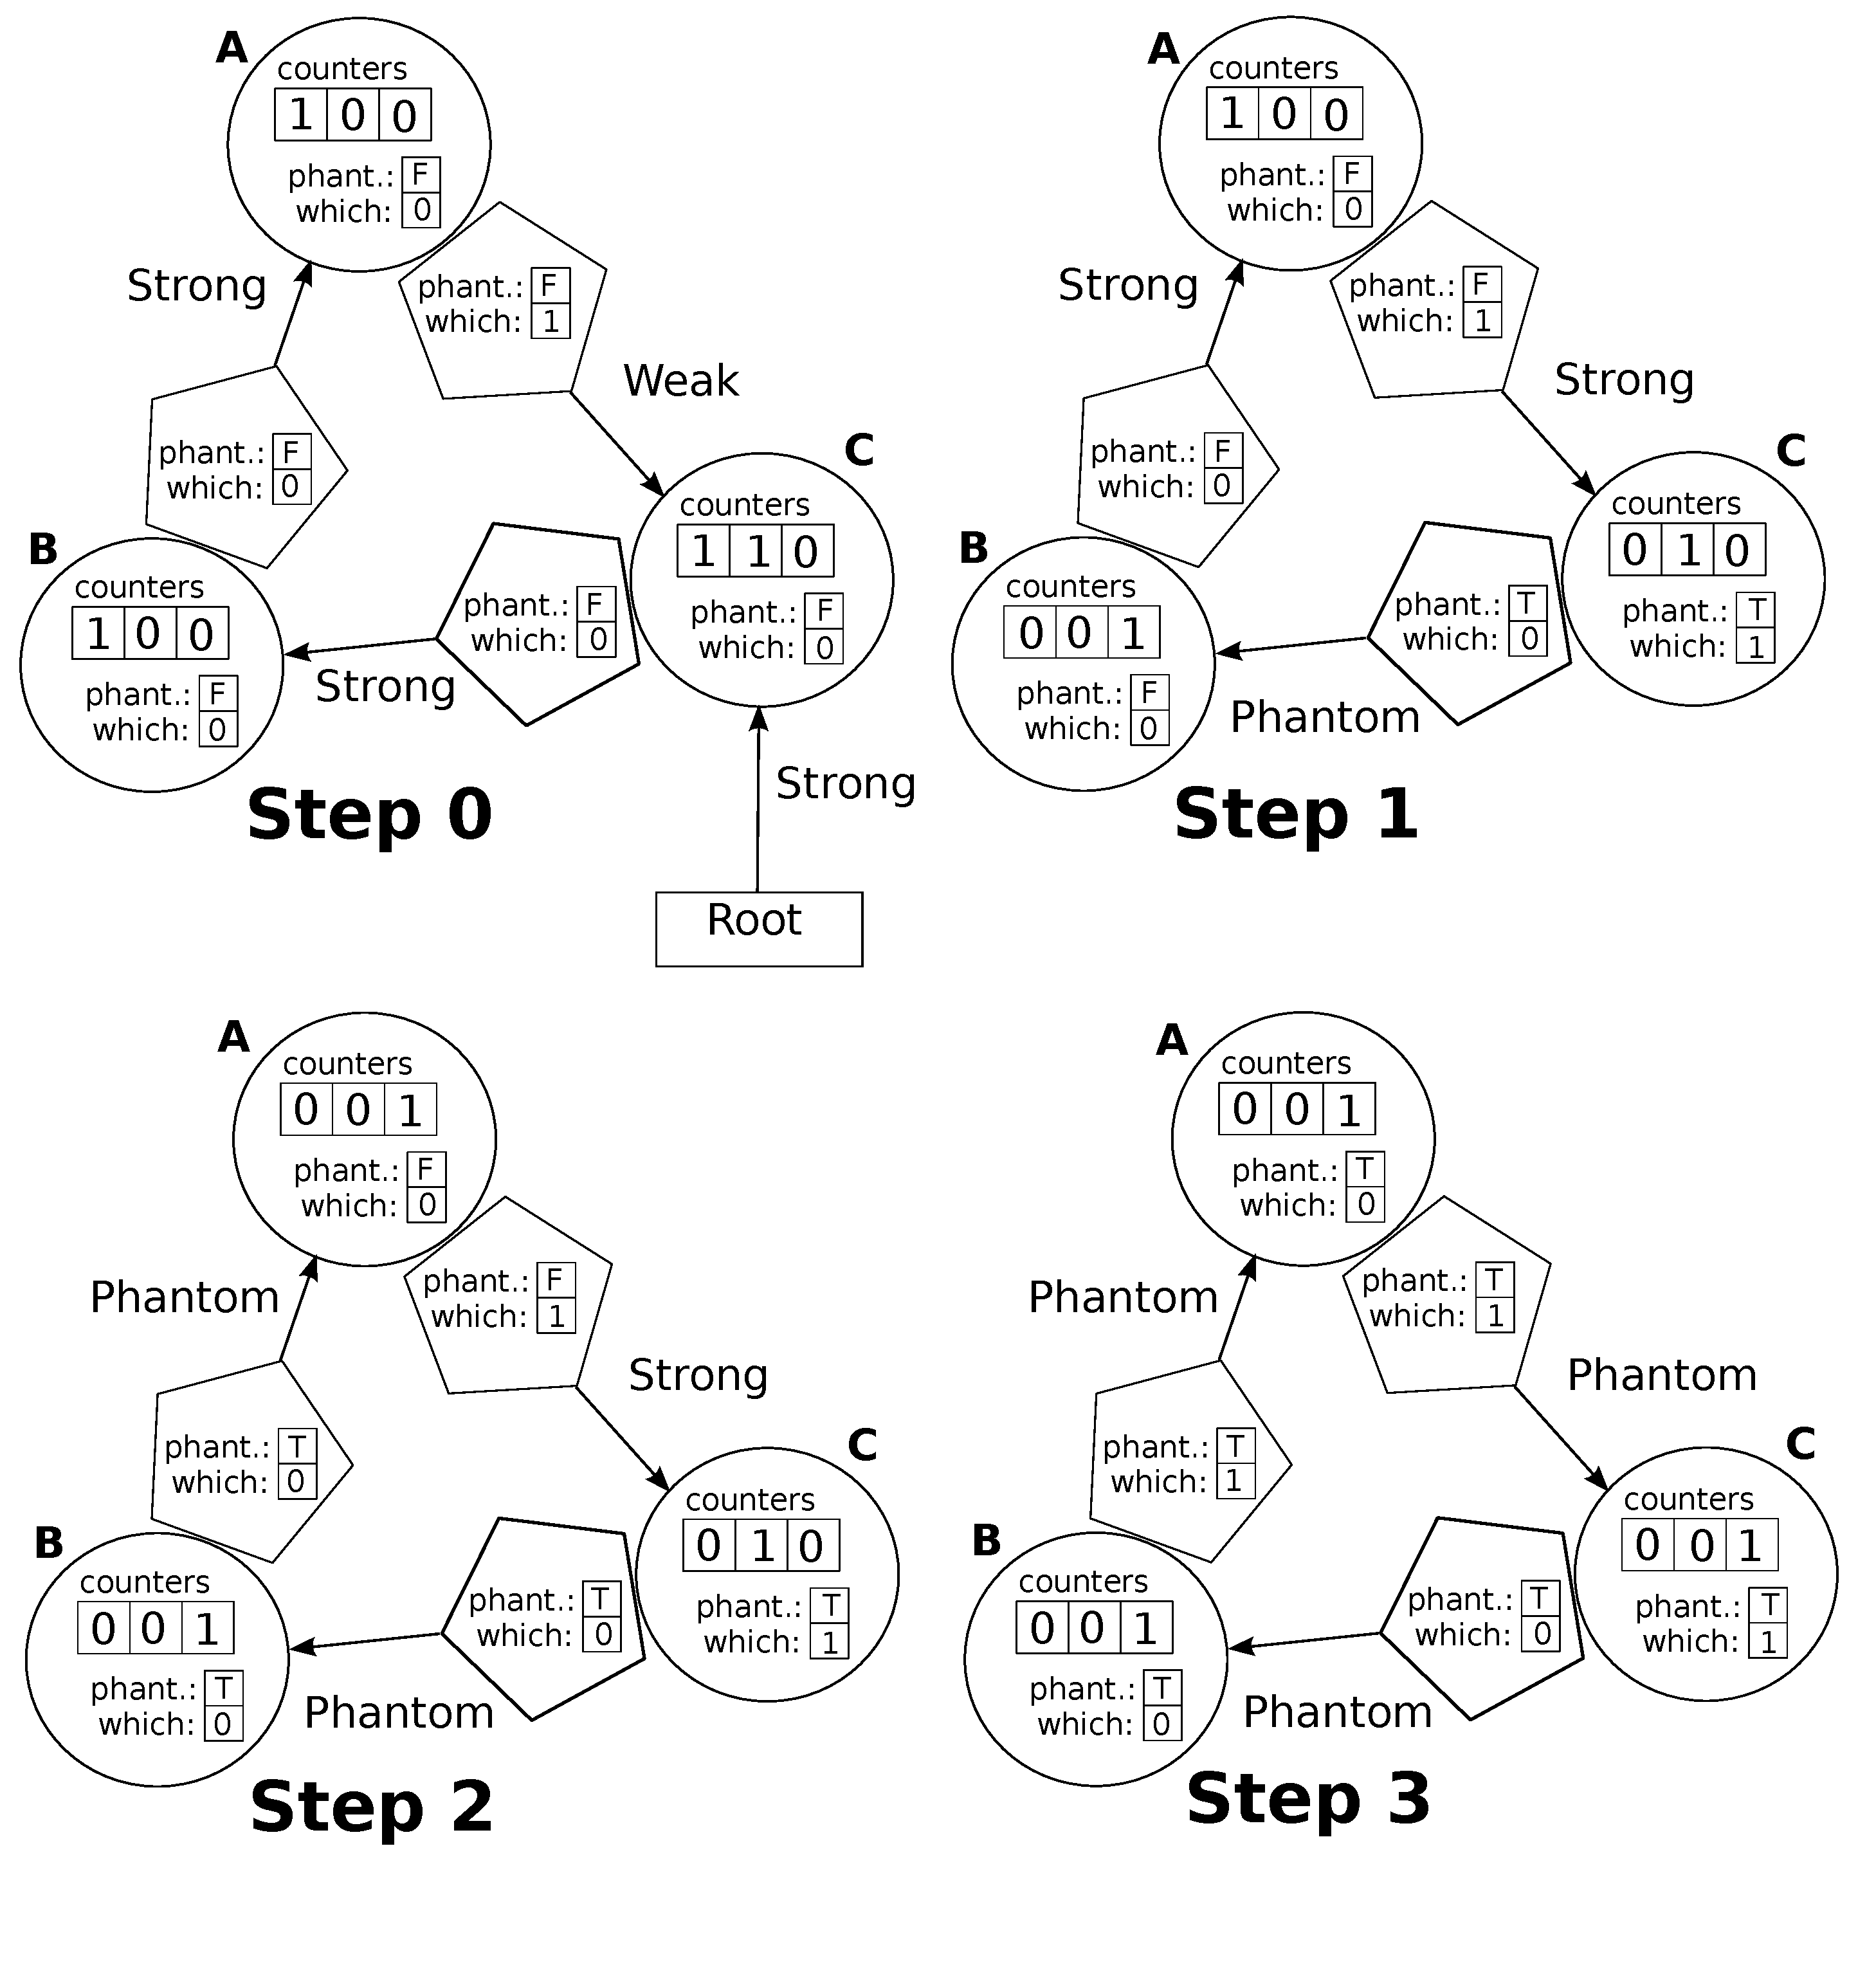
\includegraphics[height=4.5in]{figs/method}\label{fig:example1}}
  %\hspace{30pt}%
  %\subfloat[Node $u$ issues a ${\sf move}$ request]
  %{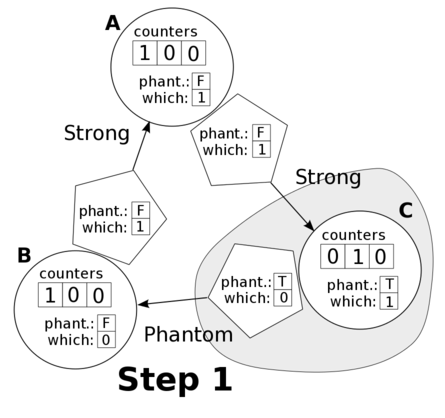
\includegraphics[height=2.0in]{figs/method1}\label{fig:example2}}\\
  %\hspace{12pt}%
  %\subfloat[The request continues up phase]
  %{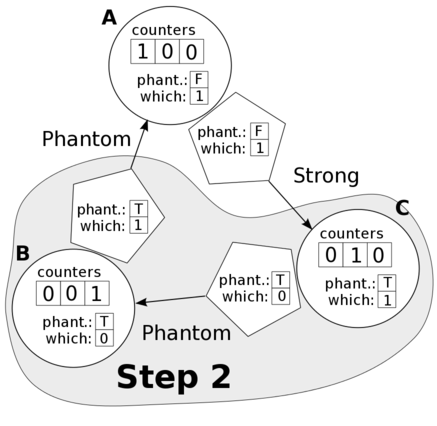
\includegraphics[height=2.0in]{figs/method2}\label{fig:example3}}
  %\hspace{30pt}%
  %\subfloat[Directory path found, new owner node $u$]
  %{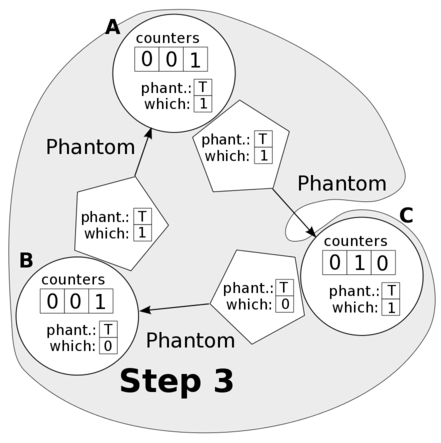
\includegraphics[height=2.0in]{figs/method3}\label{fig:example4}}
  \caption{Reclaiming a cycle with three objects}%
  \label{ex1}
\end{figure*}

\begin{figure*}[!t]
  \centering
  %\subfloat[Initially, the owner node $v$ publishes the object]
  {\includegraphics[height=2.0in]{figs/doublylinkedlist}\label{fig:example2}}
 \caption{Doubly-linked list}%
  \label{ex2}
\end{figure*}

%\begin{figure}
%\centering
%\begin{minipage}{.167\textwidth}
%    \centering
%    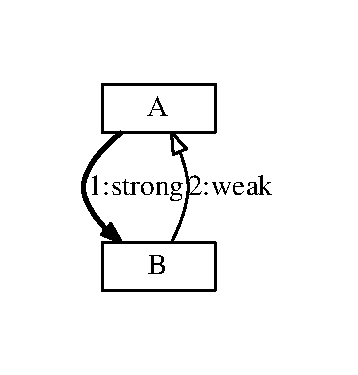
\includegraphics[width=1.0\textwidth]{figs/ex1step0}
%    %\caption{ }
%\end{minipage}%
%\begin{minipage}{.166\textwidth}
%    \centering
%    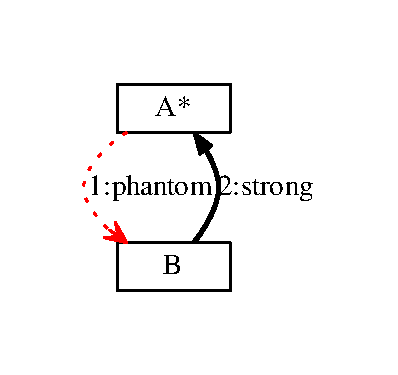
\includegraphics[width=1.0\textwidth]{figs/ex1step1}
%    %\caption{ }
%\end{minipage}%
%\begin{minipage}{.167\textwidth}
%    \centering
%    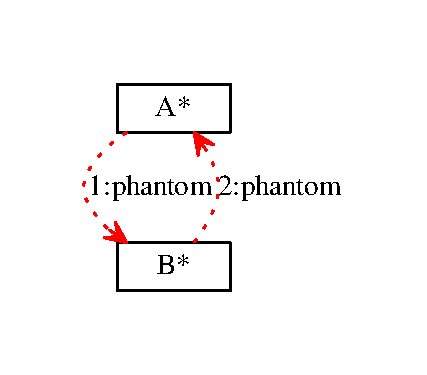
\includegraphics[width=1.0\textwidth]{figs/ex1step2}
%    %\caption{ }
%\end{minipage}%
%\end{figure}


\begin{comment}
\begin{figure}
\centering
\begin{minipage}{.167\textwidth}
    \centering
    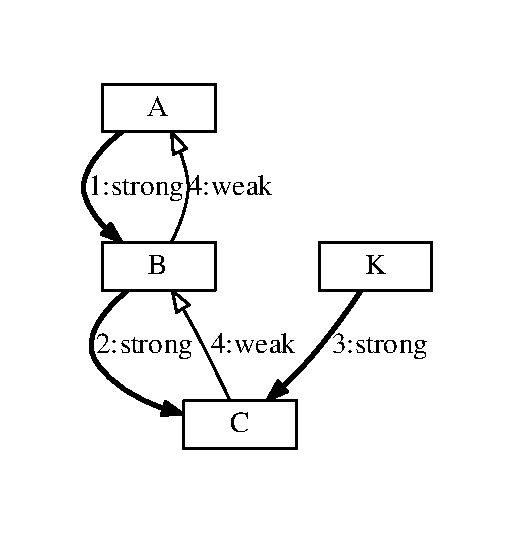
\includegraphics[width=1.0\textwidth]{figs/ex3step0}
    %\caption{ }
\end{minipage}%
\begin{minipage}{.166\textwidth}
    \centering
    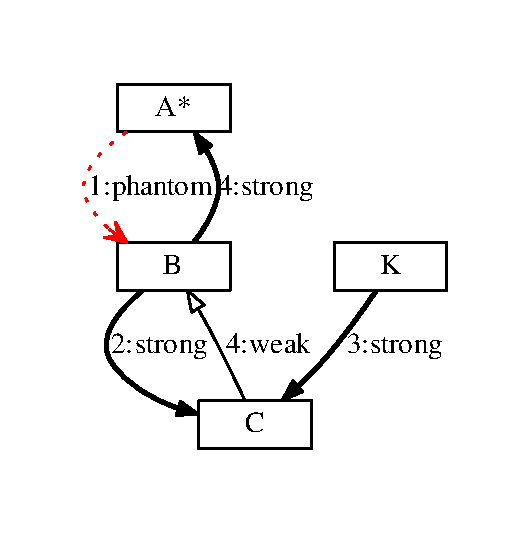
\includegraphics[width=1.0\textwidth]{figs/ex3step1}
    %\caption{ }
\end{minipage}%
\begin{minipage}{.167\textwidth}
    \centering
    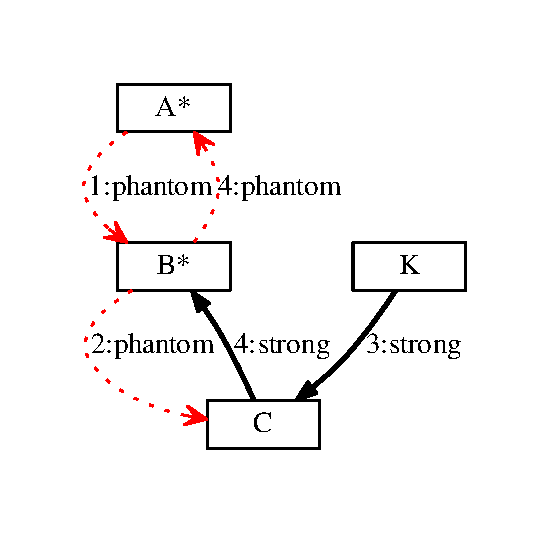
\includegraphics[width=1.0\textwidth]{figs/ex3step2}
    %\caption{ }
\end{minipage}

\begin{minipage}{.167\textwidth}
    \centering
    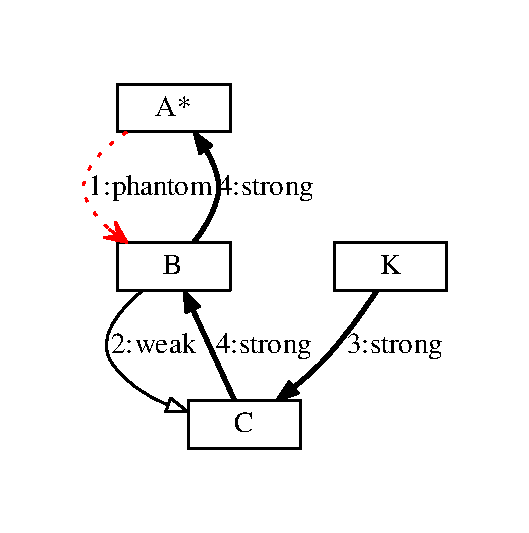
\includegraphics[width=1.0\textwidth]{figs/ex3step3}
    %\caption{ }
\end{minipage}%
\begin{minipage}{.166\textwidth}
    \centering
    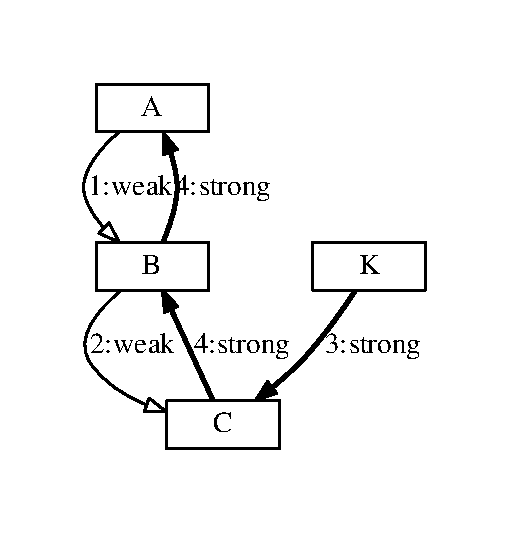
\includegraphics[width=1.0\textwidth]{figs/ex3step4}
    %\caption{ }
\end{minipage}%
\label{ex3}
\caption{Rebalancing a Doubly-Linked List}
\end{figure}
\end{comment}


\begin{figure*}[!t]
  \centering
  %\subfloat[Initially, the owner node $v$ publishes the object]
  {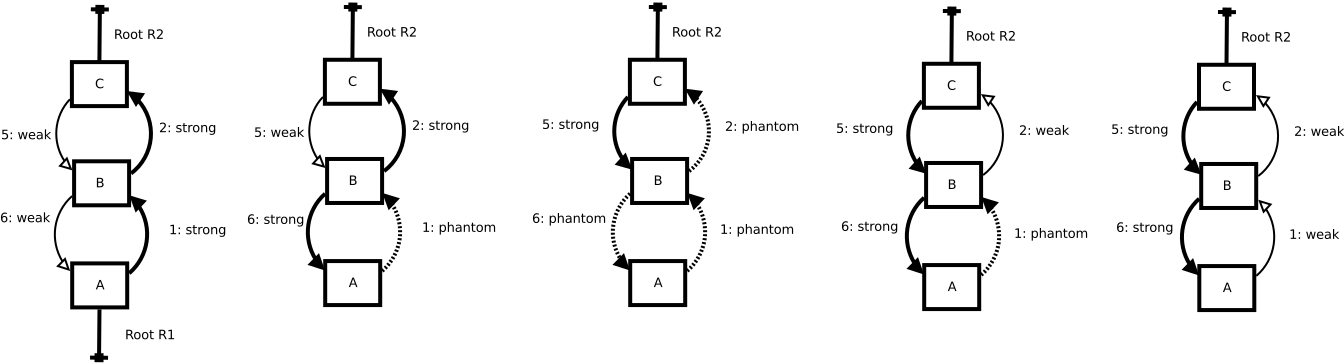
\includegraphics[height=2.0in]{figs/recoveringdbl}}%\label{fig:example1}}

  \caption{Rebalancing a doubly-linked list}%
  \label{ex3}
\end{figure*}


\subsection{Example: A Doubly-Linked List}

The doubly linked list depicted in Fig.~\ref{ex2} is a classic
example for garbage collection systems. The structure consists of
6 links, and the collector marks all the links as phantoms in 8
steps.

This figure contains much less detail than Fig.~\ref{ex1}, which
is necessary for a more complex figure.

%There are several options to choose from in deciding
%how to represent this particular structure in memory, but this
%example should suffice to enable the reader to work
%through additional similar examples.

% \begin{comment}
% \begin{figure}
% \centering
% \begin{minipage}{.167\textwidth}
%     \centering
%     \includegraphics[width=1.0\textwidth]{figs/doublylinkedlist}
%     %\caption{ }
% \end{minipage}%
%\begin{minipage}{.167\textwidth}
%   \centering
%    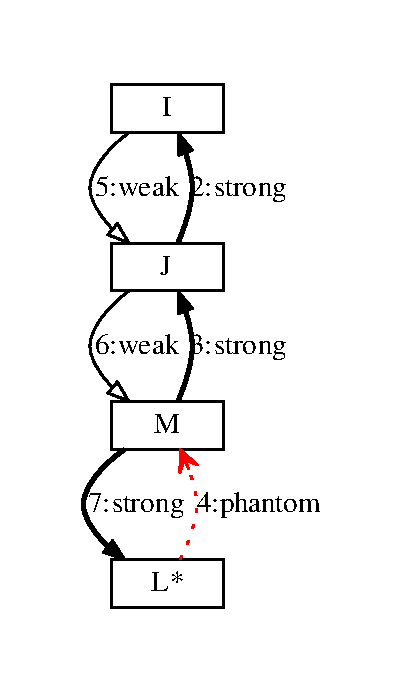
\includegraphics[width=1.0\textwidth]{figs/ex2step1}
%    %\caption{ }
%\end{minipage}%
%\begin{minipage}{.166\textwidth}
%    \centering
%    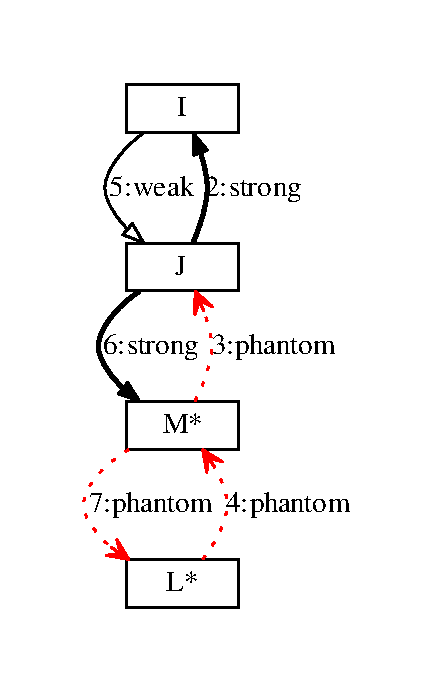
\includegraphics[width=1.0\textwidth]{figs/ex2step2}
%    %\caption{ }
%\end{minipage}

%\begin{minipage}{.167\textwidth}
%    \centering
%    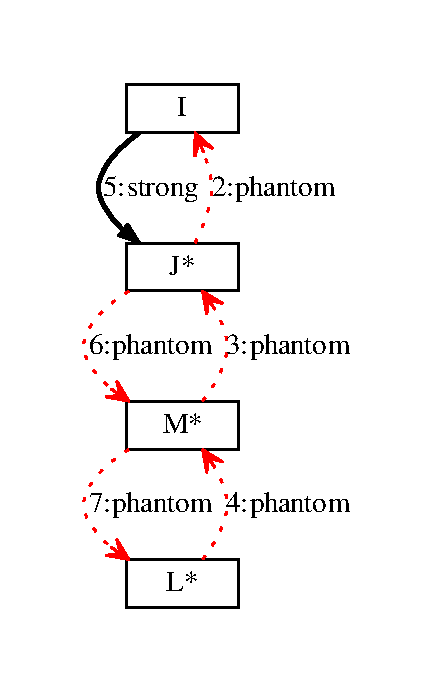
\includegraphics[width=1.0\textwidth]{figs/ex2step3}
%    %\caption{ }
%\end{minipage}%
%\begin{minipage}{.167\textwidth}
%    \centering
%    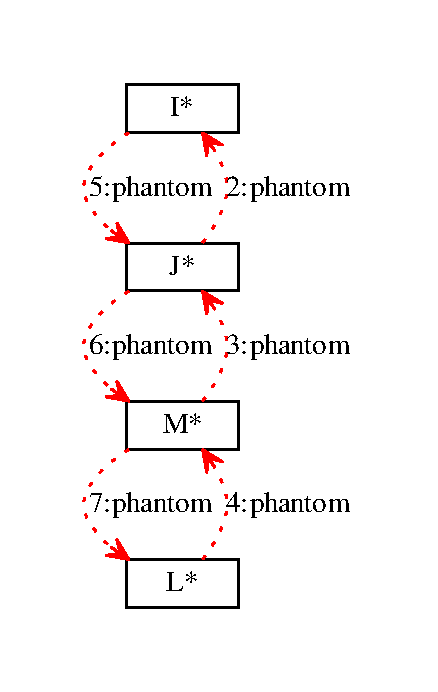
\includegraphics[width=1.0\textwidth]{figs/ex2step4}
%    %\caption{ }
%\end{minipage}%
%\label{ex2}
%\caption{Reclaiming a double cycle.}
% \end{figure}
% \end{comment}

% \begin{figure*}[!t]
%   \centering
%   %\subfloat[Initially, the owner node $v$ publishes the object]
%   {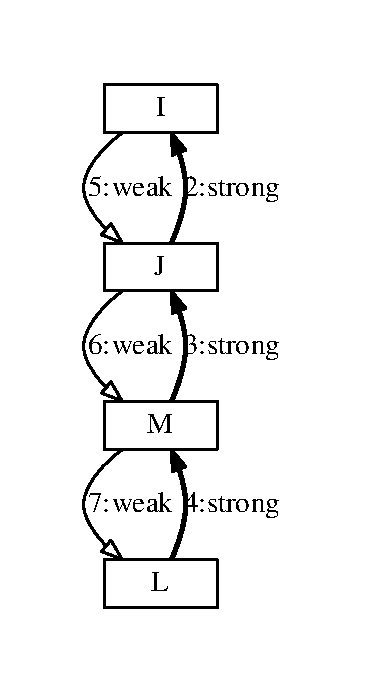
\includegraphics[height=1.6in]{figs/ex2step0}}%\label{fig:example1}}
%   \hspace{12pt}%
%   %\subfloat[Node $u$ issues a ${\sf move}$ request]
%   {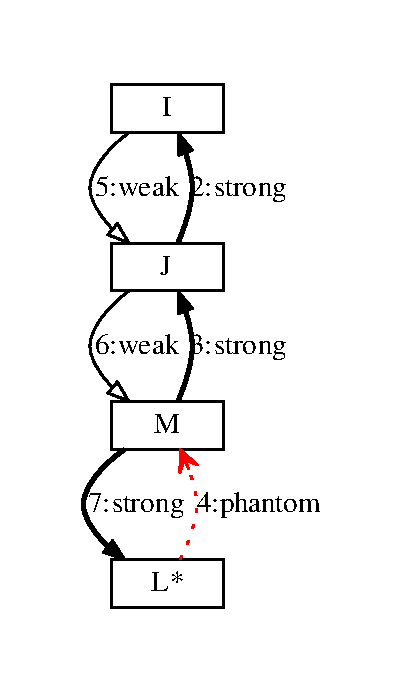
\includegraphics[height=1.6in]{figs/ex2step1}}%\label{fig:example2}}
%   \hspace{12pt}%
%   %\subfloat[The request continues up phase]
%   {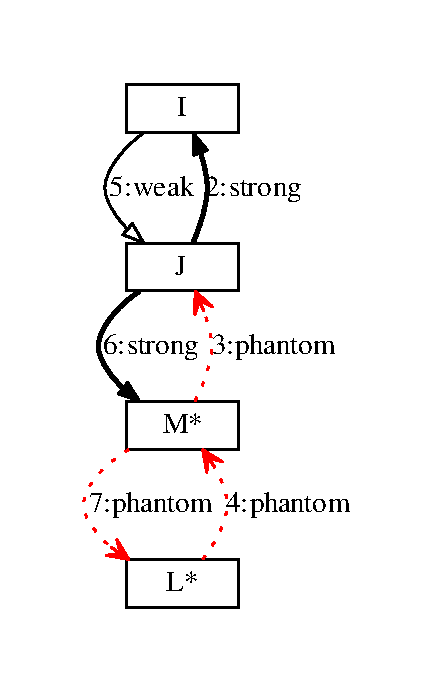
\includegraphics[height=1.6in]{figs/ex2step2}}%\label{fig:example3}}
%   \hspace{12pt}%
%   %\subfloat[Directory path found, new owner node $u$]
%   {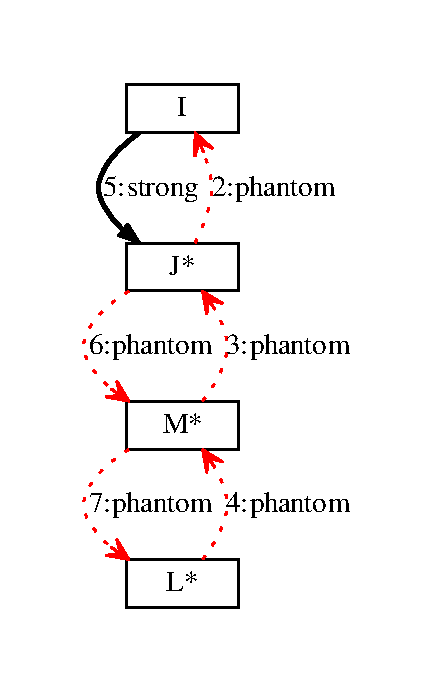
\includegraphics[height=1.6in]{figs/ex2step3}}%\label{fig:example4}}
%   \hspace{12pt}%
%   %\subfloat[Directory path found, new owner node $u$]
%   {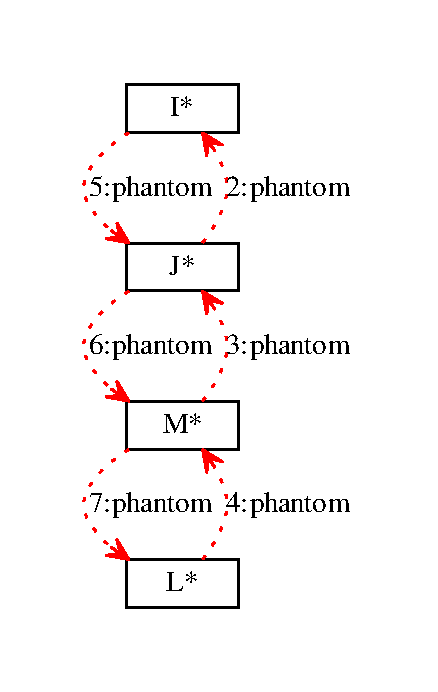
\includegraphics[height=1.6in]{figs/ex2step4}}%\label{fig:example4}}
%   \caption{Reclaiming a double cycle}%
%   \label{ex2}
% \end{figure*}

\subsection{Example: Rebalancing A Doubly-Linked List}

Fig.~\ref{ex3} represents a worst case scenario for our algorithm. As a
result of losing root $R1$, the
strong links are pointing in exactly the wrong direction to provide
support across
an entire chain of double links. During $Phantomization$, each
of the objects in the list must convert its links to phantoms,
but nothing is deleted. $Phantomization$ is complete in the third
figure from the left, and $Recovery$ begins.
The fourth step in the figure, when link 6 is converted from phantom to weak
marks the first phase of the recovery.



\subsection{Example: Recovering Without Detecting a Cycle}

In Fig.~\ref{prove} we see the situation where the collector recovers from the
loss of a strong link without searching the entire cycle. When root $R1$ is removed,
node $A$ becomes phantomized. It turns its incoming link (link $1$) to strong,
and phantomizes its outgoing link (link $2$), but
then the phantomization process ends. Recovery is successful, because $A$ has strong
support, and it rebuilds its outgoing link as weak. At this point, collection
operations are finished.

Unlike the doubly-linked list example above, this case describes an optimal
situation for our garbage collection system.

\section{Concurrency Issues}

%Note that the algorithm section omits the actual calls to lock and unlock present in our fine-grained parallel prototype.
This section provides details of the implementation.
%A reference implementation is also provided ~\cite{url:refimpl}.\todo{Make public repo}
%\update{What about we provide implementation link here. Currently it is withheld for supporting double-blind review. I think the link will make our case stronger and it does not reveal our identity directly.}

\subsection{The Single-Threaded Collector}
There are several methods by which the collector may be
allowed to interact concurrently with a live system. The first, and most straightforward
implementation, is to use a single garbage collection thread to manage nontrivial
collection operations. This technique has the advantage of limiting the amount
of computational power the garbage collector may use to perform its work.

For the collection process to work, phantomization must run to completion before
recovery is attempted, and recovery must run to completion before cleanup can
occur. To preserve this ordering in a live system,
whenever an operation would remove the last strong link
to an object with weak or phantom references, the link is instead transferred
to the collector, enabling it to perform phantomization at an appropriate time.
%See Algorithms.~\ref{algorithm:linkfree} and~\ref{algorithm:addtocollector}.

%In Algorithm~\ref{algorithm:addtocollector}, we see that
After the strong link is processed, the garbage collector needs to create a phantom
link to hold onto the object while it performs its processing, to ensure the
collector itself doesn't try to use a deleted object.

Another point of synchronization is the creation of new links. If the
source of the link is a phantomized node, the link is created in the phantomized
state. %See Algorithm~\ref{algorithm:linkset}.

With these relatively straightforward changes, the single-threaded garbage collector
may interact freely with a live system.

%Note that in the following sections, locks are always obtained in canonical order that avoids deadlocks. Unlock methods unlock the last set of items that were locked.

The lists on the collectors are thread-safe.

The collector object is itself managed by a simple reference count. Code for incrementing and decrementing this count is not explicitly present in the code below.

A reference implementation is also provided ~\cite{url:refimpl}.

\begin{algorithm}[ht]
{\small
\tcp{LinkSet creates a new link,
  and decides the type of the link to create.}
{\bf LinkSet(link,node)}:\\
\quad {lock (link.Source,node)}\\
\quad {\bf if} node == NULL {\bf then}\\
\quad \quad LinkFree(link)\\
\quad \quad link.Target = NULL\\
\quad {\bf EndIf}\\
\quad {\bf if} link.Target == node {\bf then}\\
\quad \quad {\bf Return}\\
\quad {\bf EndIf}\\
\quad oldLink = copy(link) \\
\quad link.Target = node\\
\quad {\bf If} link.Source.Phantomized {\bf then}\\
\quad \quad MergeCollectors(link.Source, link.Target)\\
\quad \quad link.PhantomCount++\\
\quad \quad link.Phantomized = True\\
\quad {\bf ElseIf} link.Source == node {\bf then}\\
\quad \quad link.Which = 1 - node.Which\\
\quad \quad node.Count[link.Which]++\\
\quad {\bf ElseIf} node.Links not initialized {\bf then}\\
\quad \quad node.Count[link.Which]++\\
\quad \quad link.Which = node.Which\\
\quad {\bf Else}\\
\quad \quad link.which = 1 - node.Which\\
\quad \quad node.Count[link.Which]++\\
\quad {\bf EndIf}\\
\quad {\bf If} oldLink != NULL\\
\quad \quad LinkFree(oldLink)\\
\quad  {unlock()}\\
}
\caption{LinkSet}
\label{single:algorithm:linkset}
\end{algorithm}
\setlength{\textfloatsep}{0pt}
\begin{algorithm}[ht]
{\small
\tcp{Freeing a link is usually just the decrement of a reference count, but
if it is the last strong count, this could potentially start a Phantomization process.}
%\begin{multicols}{2}
% \tcp{$R$ and $S$ are objects currently in use.}
{\bf LinkFree(link)}:\\
% \tcp*[f]{Create a pointer from object $R$ to some free object}\\
{\Indp
{lock(link.Source,link.Target)}\\
{\bf If} link.Target == NULL {\bf then}\\
\quad {\bf Return}\\
{\bf EndIf}\\
{\bf If} link.Phantomized {\bf then}\\
\quad DecPhantom(link.Target)\\
{\bf Else}\\
\quad link.Target.Count[link.Which]-\,-\\
\quad {\bf If} link.Target.Count[link.Which] == 0 {\bf And} \\
\quad \quad \quad link.Target.Which == link.Which {\bf then}\\
\quad \quad {\bf If} link.Target.Count[1-link.Target.Which] == 0 {\bf And} \\
\quad \quad \quad \quad link.Target.PhantomCount == 0 {\bf then}\\
\quad \quad \quad Delete(node)\\
\quad \quad \quad link.Target = NULL\\
\quad \quad {\bf Else} \\
\quad \quad \quad {\bf If} link.Target.Collector == NULL {\bf then}\\
\quad \quad \quad \quad link.Target.Collector = new Collector()\\
\quad \quad \quad {\bf EndIf}\\
\quad \quad \quad AddToCollector(link.Target)\\
\quad \quad {\bf EndIf} \\
\quad {\bf EndIf}\\
{\bf EndIf}\\
{unlock()}\\
}
}
\caption{LinkFree}
\label{algorithm:linkfree}
\end{algorithm}
\setlength{\textfloatsep}{0pt}
\begin{algorithm}[ht]
{\small
%\begin{multicols}{2}
% \tcp{$R$ and $S$ are objects currently in use.}
% \tcp*[f]{Create a pointer from object $R$ to some free object}\\
\tcp{Adding an object to the collector puts back the strong
count, effectively transferring the source of the strong link
to the collector. It also adds a phantom count, which helps
prevent the clearing of the Collector field.}
{\bf AddToCollector(node)}:\\
{\Indp
{\bf While} True\\
\quad {lock(node,node.Collector)}\\
\quad {\bf If} node.Collector.Forward != NULL {\bf then}\\
\quad \quad node.Collector = node.Collector.Forward\\
\quad {\bf Else}\\
\quad \quad node.Count[node.Which]++\\
\quad \quad node.PhantomCount++\\
\quad \quad node.Collector.CollectionList.append(node)\\
\quad \quad {\bf Break}\\
\quad {\bf EndIf}\\
\quad {unlock()}\\
{\bf EndWhile}\\
}
}
\caption{AddToCollector}
\label{single:algorithm:addtocollector}
\end{algorithm}
%\end{multicols}
\setlength{\textfloatsep}{0pt}
\begin{algorithm}[ht]
{\small
%\begin{multicols}{2}
\tcp{The collector takes away the strong link it made in
AddToCollector().
}
{\bf PhantomizeNode(node,collector)}:\\
{\Indp
{lock(node)}\\
{\bf While} collector.Forward != NULL\\
\quad collector = collector.Forward\\
{\bf EndWhile}\\
node.Collector = collector\\
node.Count[node.Which]-\,-\\
\quad // Prevent deletion while the\\
\quad // node is managed by the Collector\\
{\bf Let} phantomize = False\\
{\bf If} node.Count[node.Which] $>$ 0 {\bf then}\\
\quad {\bf Return}\\
{\bf Else}\\
\quad {\bf If} node.Count[1-node.Which] $>$ 0 {\bf then}\\
\quad \quad node.Which = 1-node.Which\\
\quad {\bf EndIf}\\
\quad {\bf If} {\bf Not} node.Phantomized {\bf then}\\
\quad \quad node.Phantomized = True\\
\quad \quad node.PhantomizationComplete = False\\
\quad \quad phantomize = True\\
\quad {\bf EndIf}\\

{\bf EndIf}\\
{\bf Let} links = NULL \\
{\bf If} phantomize {\bf then}\\
\quad links = copy(node.Links)\\
{\bf EndIf}\\
{unlock()}\\
{\bf ForEach} outgoing link in links\\
\quad PhantomizeLink(link)\\
{\bf EndFor}\\
lock(node)\\
{node.PhantomizationComplete = True}\\
unlock()\\
}
%\end{multicols}
}
\caption{PhantomizeNode}
\label{algorithm:phantomizenode}
\end{algorithm}
\setlength{\textfloatsep}{0pt}
\begin{algorithm}[ht]
{\small
%\begin{multicols}{2}
\tcp{This method describes the
work to be carried out by a
garbage collection thread. Live
objects pointing to this collector, or
Forward pointers from other collectors
contribute to the RefCount field on
the Collector.}
{\bf Collector.Main()}:\\
{\Indp
{\bf While} True \\
\quad WaitFor(Collector.RefCount == 0 {\bf Or} Work to do)\\
\quad {\bf If} Collector.RefCount == 0 {\bf And} No work to do {\bf then}\\
\quad \quad {\bf Break}\\
\quad {\bf EndIf}\\
\quad {\bf While} Collector.MergedList.size() $>$ 0\\
\quad \quad Let node = Collector.MergedList.pop()\\
\quad \quad Collector.RecoveryList.append(node)\\
\quad {\bf EndWhile}\\
\quad {\bf While} Collector.CollectionList.size() $>$ 0\\
\quad \quad Let node = Collector.CollectionList.pop()\\
\quad \quad PhantomizeNode(node,Collector)\\
\quad \quad Collector.RecoveryList.append(node)\\
\quad {\bf EndWhile}\\
\quad {\bf While} Collector.RecoveryList.size() $>$ 0\\
\quad \quad Let node = Collector.RecoveryList.pop()\\
\quad \quad RecoverNode(node)\\
\quad \quad Collector.CleanList.append(node)\\
\quad {\bf EndWhile}\\
\quad {\bf While} Collector.RebuildList.size() $>$ 0\\
\quad \quad Let node = Collector.RebuildList.pop()\\
\quad \quad RecoverNode(node)\\
\quad {\bf EndWhile}\\
\quad {\bf While} Collector.CleanList.size() $>$ 0\\
\quad \quad Let node = Collector.CleanList.pop()\\
\quad \quad CleanNode(node)\\
\quad {\bf EndWhile}\\
{\bf EndWhile}\\
}
}
\caption{Collector.Main}
\label{algorithm:main}
\end{algorithm}
\setlength{\textfloatsep}{0pt}
\begin{algorithm}[ht]
{\small
%\begin{multicols}{2}
{\bf PhantomizeLink(link)}:\\
{\Indp
 {lock(link.Source,link.Target)}\\
 {\bf If} link.Target == NULL {\bf then}\\
\quad  {unlock()}\\
 \quad {\bf Return}\\
 {\bf EndIf}\\
{\bf If} link.Phantomized {\bf then}\\
\quad  {unlock()}\\
\quad {\bf Return} \\
{\bf EndIf}\\
link.Target.PhantomCount++\\
link.Phantomized = True\\
linkFree(link)\\
MergeCollectors(link.Source, link.Target)\\
 {unlock()}\\
}
}
\caption{PhantomizeLink}
\label{single:algorithm:phantomizelink}
\end{algorithm}
\setlength{\textfloatsep}{0pt}
\begin{algorithm}[ht]
{\small
%\begin{multicols}{2}
\tcp{DecPhantom is responsible for removing any reference to
the collector.}
{\bf DecPhantom(node)}:\\
{\Indp
 {lock(node)}\\
node.PhantomCount- -\\
{\bf If} node.PhantomCount == 0 {\bf then}\\
\quad {\bf If} node.Count[node.Which]== 0 {\bf And}\\
\quad \quad \quad node.Count[1-node.Which] == 0 {\bf then}\\
\quad \quad Delete(node)\\
\quad {\bf Else}\\
\quad \quad node.Collector = NULL\\
\quad {\bf EndIf}\\
{\bf EndIf}\\
 {unlock()}\\
}
}
\caption{DecPhantom}
\label{single:algorithm:decPhantom}
\end{algorithm}
\setlength{\textfloatsep}{0pt}

\begin{algorithm}[ht]
{\small
%\begin{multicols}{2}
{\bf RecoverNode(node)}:\\
{\Indp
 {lock(node)}\\
{\bf Let} links = NULL\\
{\bf If} node.Count[node.Which] $>$ 0 {\bf then}\\
\quad WaitFor(node.PhantomizationComplete == True)\\
\quad node.Phantomized = False\\
\quad links = copy(node.Links)\\
{\bf EndIf}\\
 {unlock()}\\
{\bf ForEach} link in links \\
\quad Rebuild(link)\\
{\bf EndFor}\\
}
}
\caption{RecoverNode}
\label{algorithm:recover}
\end{algorithm}
\setlength{\textfloatsep}{0pt}

\begin{algorithm}[ht]
{\small
%\begin{multicols}{2}
{\bf Rebuild(link)}:\\
{\Indp
 {lock(link.Source,link.Target)}\\
{\bf If} link.Phantomized {\bf then}\\
\quad {\bf If} link.Target == link.Source {\bf then}\\
\quad \quad link.Which = 1- link.Target.Which\\
\quad {\bf ElseIf} link.Target.Phantomized {\bf then} \\
\quad \quad link.Which = link.Target.Which\\
\quad {\bf ElseIf} count(link.Target.Links) == 0 {\bf then}\\
\quad \quad link.Which = link.Target.Which\\
\quad {\bf Else}\\
\quad \quad link.Which = 1-link.Target.Which\\
\quad {\bf EndIf}\\
\quad link.Target.Count[link.Which]++\\
\quad link.Target.PhantomCount- -\\
\quad{\bf If} link.Target.PhantomCount == 0 {\bf then}\\
\quad \quad link.Target.Collector = NULL\\
\quad {\bf EndIf}\\
\quad link.Phantomized = False \\
\quad Add link.Target to Collector.RecoveryList\\
{\bf EndIf}\\
 {unlock()}\\
}
}
\caption{Rebuild}
\label{single:algorithm:rebuild}
\end{algorithm}
\setlength{\textfloatsep}{0pt}

\begin{algorithm}[ht]
{\small
%\begin{multicols}{2}
\tcp{After deleting all the outgoing links, decrement
the phantom count by one (i.e. the reference held by
the collector itself). When the last phantom count
is gone, the object is cleaned up.}
{\bf  CleanNode(node)}:\\
{\Indp
 {lock(node)}\\
{\bf Let} die = False\\
{\bf If} node.Count[node.Which]== 0 {\bf And}\\
\quad \quad node.Count[1-node.Which]== 0 {\bf then}\\
\quad  die = True\\
{\bf EndIf}\\
{unlock()}\\
{\bf If} die {\bf then}\\
\quad {\bf ForEach} link in node\\
\quad \quad LinkFree(link)\\
\quad {\bf EndFor}\\
{\bf EndIf}\\
DecPhantom(node)\\
 }
}
\caption{CleanNode}
\label{algorithm:cleanup}
\end{algorithm}
\setlength{\textfloatsep}{0pt}
\begin{algorithm}[ht]
{\small
{\bf  Delete(node)}:\\
{\Indp
\quad {\bf ForEach} link in node \\
\quad \quad LinkFree(link)\\
\quad {\bf EndFor}\\
\quad freeMem(node)\\

 }
}
\caption{Delete}
\label{algorithm:Delete}
\end{algorithm}
\setlength{\textfloatsep}{0pt}

\begin{algorithm}[ht]
{\small
%\begin{multicols}{2}
\tcp{When two collector threads
realize they are managing a common
subset of objects, one defers to
the other. The arguments, source and
target, are both nodes.}
{\bf MergeCollectors(source,target)}:\\
{\Indp
{\bf Let} s = source.Collector\\
{\bf Let} t = target.Collector\\
{\bf Let} done = False\\
{\bf If} s == NULL {\bf And} t != NULL {\bf then}\\
\quad lock(source)\\
\quad source.Collector = t\\
\quad unlock()\\
\quad {\bf Return}\\
{\bf EndIf}\\
{\bf If} s != NULL {\bf And} t == NULL {\bf then}\\
\quad lock(target)\\
\quad target.Collector = s\\
\quad unlock()\\
\quad {\bf Return}\\
{\bf EndIf}\\
{\bf If} s == NULL {\bf Or} s == NULL {\bf then}\\
\quad {\bf Return}\\
{\bf EndIf}\\
{\bf While Not} done\\
\quad  {lock(s,t,target,source)}\\
\quad {\bf If} s.Forward == t and t.Forward == NULL {\bf then}\\
\quad \quad target.Collector = s\\
\quad \quad source.Collector = s\\
\quad \quad done = True\\
\quad {\bf ElseIf} t.Forward == s and s.Forward == NULL {\bf then}\\
\quad \quad target.Collector = t\\
\quad \quad source.Collector = t\\
\quad \quad done = True\\
\quad {\bf ElseIf} t.Forward != NULL {\bf then}\\
\quad \quad t = t.Forward \\
\quad {\bf ElseIf} s.Forward != NULL {\bf then}\\
\quad \quad s = s.Forward \\
\quad {\bf Else}\\
\quad \quad Transfer s.CollectionList to t.CollectionList \\
\quad \quad Transfer s.MergedList to t.MergedList \\
\quad \quad Transfer s.RecoveryList to t.MergedList \\
\quad \quad Transfer s.RebuildList to t.RebuildList \\
\quad \quad Transfer s.CleanList to t.MergedList \\
\quad \quad target.Collector = t\\
\quad \quad source.Collector = t\\
\quad \quad done = True\\
\quad {\bf EndIf}\\
\quad unlock()\\
{\bf EndWhile} \\
}
}
\caption{MergeCollectors}
\label{algorithm:mergecollectors}
\end{algorithm}


%See appendix~\ref{singlethread} for algorithmic details.

\subsection{The Multi-Threaded Collector}

The second, and more difficult method, is to allow the collector to
use multiple threads. In this method, independent collector threads can
start and run in disjoint areas of memory. In order to prevent conflicts
from their interaction, we use a simple technique: whenever a link
connecting two collector threads is
phantomized, or when a phantom link is created by the live system connecting
subgraphs under analysis by different collector threads, the threads merge. % (see Algorithm~\ref{algorithm:mergecollectors}).
A merge is accomplished by one thread
transferring its remaining work to the other and exiting. To make this possible, each
object needs to carry a reference to the collection threads and ensure that this
reference is removed when collection operations are complete. While the addition
of a pointer may appear to be a significant increase in memory overhead, it should be noted that
the pointer need not point directly to the collector, but to an intermediate object which can
carry the phantom counter, as well as other information if desired.

An implementation of this parallelization strategy is given in pseudocode in the appendix.

%Note that in the following sections, locks are always obtained in canonical order that avoids deadlocks. Unlock methods unlock the last set of items that were locked.

The lists on the collectors are thread-safe.

The collector object is itself managed by a simple reference count. Code for incrementing and decrementing this count is not explicitly present in the code below.

A reference implementation is also provided ~\cite{url:refimpl}.

\begin{algorithm}[ht]
{\small
\tcp{LinkSet creates a new link,
  and decides the type of the link to create.}
{\bf LinkSet(link,node)}:\\
\quad {lock (link.Source,node)}\\
\quad {\bf if} node == NULL {\bf then}\\
\quad \quad LinkFree(link)\\
\quad \quad link.Target = NULL\\
\quad {\bf EndIf}\\
\quad {\bf if} link.Target == node {\bf then}\\
\quad \quad {\bf Return}\\
\quad {\bf EndIf}\\
\quad oldLink = copy(link) \\
\quad link.Target = node\\
\quad {\bf If} link.Source.Phantomized {\bf then}\\
\quad \quad MergeCollectors(link.Source, link.Target)\\
\quad \quad link.PhantomCount++\\
\quad \quad link.Phantomized = True\\
\quad {\bf ElseIf} link.Source == node {\bf then}\\
\quad \quad link.Which = 1 - node.Which\\
\quad \quad node.Count[link.Which]++\\
\quad {\bf ElseIf} node.Links not initialized {\bf then}\\
\quad \quad node.Count[link.Which]++\\
\quad \quad link.Which = node.Which\\
\quad {\bf Else}\\
\quad \quad link.which = 1 - node.Which\\
\quad \quad node.Count[link.Which]++\\
\quad {\bf EndIf}\\
\quad {\bf If} oldLink != NULL\\
\quad \quad LinkFree(oldLink)\\
\quad  {unlock()}\\
}
\caption{LinkSet}
\label{single:algorithm:linkset}
\end{algorithm}
\setlength{\textfloatsep}{0pt}
\begin{algorithm}[ht]
{\small
\tcp{Freeing a link is usually just the decrement of a reference count, but
if it is the last strong count, this could potentially start a Phantomization process.}
%\begin{multicols}{2}
% \tcp{$R$ and $S$ are objects currently in use.}
{\bf LinkFree(link)}:\\
% \tcp*[f]{Create a pointer from object $R$ to some free object}\\
{\Indp
{lock(link.Source,link.Target)}\\
{\bf If} link.Target == NULL {\bf then}\\
\quad {\bf Return}\\
{\bf EndIf}\\
{\bf If} link.Phantomized {\bf then}\\
\quad DecPhantom(link.Target)\\
{\bf Else}\\
\quad link.Target.Count[link.Which]-\,-\\
\quad {\bf If} link.Target.Count[link.Which] == 0 {\bf And} \\
\quad \quad \quad link.Target.Which == link.Which {\bf then}\\
\quad \quad {\bf If} link.Target.Count[1-link.Target.Which] == 0 {\bf And} \\
\quad \quad \quad \quad link.Target.PhantomCount == 0 {\bf then}\\
\quad \quad \quad Delete(node)\\
\quad \quad \quad link.Target = NULL\\
\quad \quad {\bf Else} \\
\quad \quad \quad {\bf If} link.Target.Collector == NULL {\bf then}\\
\quad \quad \quad \quad link.Target.Collector = new Collector()\\
\quad \quad \quad {\bf EndIf}\\
\quad \quad \quad AddToCollector(link.Target)\\
\quad \quad {\bf EndIf} \\
\quad {\bf EndIf}\\
{\bf EndIf}\\
{unlock()}\\
}
}
\caption{LinkFree}
\label{algorithm:linkfree}
\end{algorithm}
\setlength{\textfloatsep}{0pt}
\begin{algorithm}[ht]
{\small
%\begin{multicols}{2}
% \tcp{$R$ and $S$ are objects currently in use.}
% \tcp*[f]{Create a pointer from object $R$ to some free object}\\
\tcp{Adding an object to the collector puts back the strong
count, effectively transferring the source of the strong link
to the collector. It also adds a phantom count, which helps
prevent the clearing of the Collector field.}
{\bf AddToCollector(node)}:\\
{\Indp
{\bf While} True\\
\quad {lock(node,node.Collector)}\\
\quad {\bf If} node.Collector.Forward != NULL {\bf then}\\
\quad \quad node.Collector = node.Collector.Forward\\
\quad {\bf Else}\\
\quad \quad node.Count[node.Which]++\\
\quad \quad node.PhantomCount++\\
\quad \quad node.Collector.CollectionList.append(node)\\
\quad \quad {\bf Break}\\
\quad {\bf EndIf}\\
\quad {unlock()}\\
{\bf EndWhile}\\
}
}
\caption{AddToCollector}
\label{single:algorithm:addtocollector}
\end{algorithm}
%\end{multicols}
\setlength{\textfloatsep}{0pt}
\begin{algorithm}[ht]
{\small
%\begin{multicols}{2}
\tcp{The collector takes away the strong link it made in
AddToCollector().
}
{\bf PhantomizeNode(node,collector)}:\\
{\Indp
{lock(node)}\\
{\bf While} collector.Forward != NULL\\
\quad collector = collector.Forward\\
{\bf EndWhile}\\
node.Collector = collector\\
node.Count[node.Which]-\,-\\
\quad // Prevent deletion while the\\
\quad // node is managed by the Collector\\
{\bf Let} phantomize = False\\
{\bf If} node.Count[node.Which] $>$ 0 {\bf then}\\
\quad {\bf Return}\\
{\bf Else}\\
\quad {\bf If} node.Count[1-node.Which] $>$ 0 {\bf then}\\
\quad \quad node.Which = 1-node.Which\\
\quad {\bf EndIf}\\
\quad {\bf If} {\bf Not} node.Phantomized {\bf then}\\
\quad \quad node.Phantomized = True\\
\quad \quad node.PhantomizationComplete = False\\
\quad \quad phantomize = True\\
\quad {\bf EndIf}\\

{\bf EndIf}\\
{\bf Let} links = NULL \\
{\bf If} phantomize {\bf then}\\
\quad links = copy(node.Links)\\
{\bf EndIf}\\
{unlock()}\\
{\bf ForEach} outgoing link in links\\
\quad PhantomizeLink(link)\\
{\bf EndFor}\\
lock(node)\\
{node.PhantomizationComplete = True}\\
unlock()\\
}
%\end{multicols}
}
\caption{PhantomizeNode}
\label{algorithm:phantomizenode}
\end{algorithm}
\setlength{\textfloatsep}{0pt}
\begin{algorithm}[ht]
{\small
%\begin{multicols}{2}
\tcp{This method describes the
work to be carried out by a
garbage collection thread. Live
objects pointing to this collector, or
Forward pointers from other collectors
contribute to the RefCount field on
the Collector.}
{\bf Collector.Main()}:\\
{\Indp
{\bf While} True \\
\quad WaitFor(Collector.RefCount == 0 {\bf Or} Work to do)\\
\quad {\bf If} Collector.RefCount == 0 {\bf And} No work to do {\bf then}\\
\quad \quad {\bf Break}\\
\quad {\bf EndIf}\\
\quad {\bf While} Collector.MergedList.size() $>$ 0\\
\quad \quad Let node = Collector.MergedList.pop()\\
\quad \quad Collector.RecoveryList.append(node)\\
\quad {\bf EndWhile}\\
\quad {\bf While} Collector.CollectionList.size() $>$ 0\\
\quad \quad Let node = Collector.CollectionList.pop()\\
\quad \quad PhantomizeNode(node,Collector)\\
\quad \quad Collector.RecoveryList.append(node)\\
\quad {\bf EndWhile}\\
\quad {\bf While} Collector.RecoveryList.size() $>$ 0\\
\quad \quad Let node = Collector.RecoveryList.pop()\\
\quad \quad RecoverNode(node)\\
\quad \quad Collector.CleanList.append(node)\\
\quad {\bf EndWhile}\\
\quad {\bf While} Collector.RebuildList.size() $>$ 0\\
\quad \quad Let node = Collector.RebuildList.pop()\\
\quad \quad RecoverNode(node)\\
\quad {\bf EndWhile}\\
\quad {\bf While} Collector.CleanList.size() $>$ 0\\
\quad \quad Let node = Collector.CleanList.pop()\\
\quad \quad CleanNode(node)\\
\quad {\bf EndWhile}\\
{\bf EndWhile}\\
}
}
\caption{Collector.Main}
\label{algorithm:main}
\end{algorithm}
\setlength{\textfloatsep}{0pt}
\begin{algorithm}[ht]
{\small
%\begin{multicols}{2}
{\bf PhantomizeLink(link)}:\\
{\Indp
 {lock(link.Source,link.Target)}\\
 {\bf If} link.Target == NULL {\bf then}\\
\quad  {unlock()}\\
 \quad {\bf Return}\\
 {\bf EndIf}\\
{\bf If} link.Phantomized {\bf then}\\
\quad  {unlock()}\\
\quad {\bf Return} \\
{\bf EndIf}\\
link.Target.PhantomCount++\\
link.Phantomized = True\\
linkFree(link)\\
MergeCollectors(link.Source, link.Target)\\
 {unlock()}\\
}
}
\caption{PhantomizeLink}
\label{single:algorithm:phantomizelink}
\end{algorithm}
\setlength{\textfloatsep}{0pt}
\begin{algorithm}[ht]
{\small
%\begin{multicols}{2}
\tcp{DecPhantom is responsible for removing any reference to
the collector.}
{\bf DecPhantom(node)}:\\
{\Indp
 {lock(node)}\\
node.PhantomCount- -\\
{\bf If} node.PhantomCount == 0 {\bf then}\\
\quad {\bf If} node.Count[node.Which]== 0 {\bf And}\\
\quad \quad \quad node.Count[1-node.Which] == 0 {\bf then}\\
\quad \quad Delete(node)\\
\quad {\bf Else}\\
\quad \quad node.Collector = NULL\\
\quad {\bf EndIf}\\
{\bf EndIf}\\
 {unlock()}\\
}
}
\caption{DecPhantom}
\label{single:algorithm:decPhantom}
\end{algorithm}
\setlength{\textfloatsep}{0pt}

\begin{algorithm}[ht]
{\small
%\begin{multicols}{2}
{\bf RecoverNode(node)}:\\
{\Indp
 {lock(node)}\\
{\bf Let} links = NULL\\
{\bf If} node.Count[node.Which] $>$ 0 {\bf then}\\
\quad WaitFor(node.PhantomizationComplete == True)\\
\quad node.Phantomized = False\\
\quad links = copy(node.Links)\\
{\bf EndIf}\\
 {unlock()}\\
{\bf ForEach} link in links \\
\quad Rebuild(link)\\
{\bf EndFor}\\
}
}
\caption{RecoverNode}
\label{algorithm:recover}
\end{algorithm}
\setlength{\textfloatsep}{0pt}

\begin{algorithm}[ht]
{\small
%\begin{multicols}{2}
{\bf Rebuild(link)}:\\
{\Indp
 {lock(link.Source,link.Target)}\\
{\bf If} link.Phantomized {\bf then}\\
\quad {\bf If} link.Target == link.Source {\bf then}\\
\quad \quad link.Which = 1- link.Target.Which\\
\quad {\bf ElseIf} link.Target.Phantomized {\bf then} \\
\quad \quad link.Which = link.Target.Which\\
\quad {\bf ElseIf} count(link.Target.Links) == 0 {\bf then}\\
\quad \quad link.Which = link.Target.Which\\
\quad {\bf Else}\\
\quad \quad link.Which = 1-link.Target.Which\\
\quad {\bf EndIf}\\
\quad link.Target.Count[link.Which]++\\
\quad link.Target.PhantomCount- -\\
\quad{\bf If} link.Target.PhantomCount == 0 {\bf then}\\
\quad \quad link.Target.Collector = NULL\\
\quad {\bf EndIf}\\
\quad link.Phantomized = False \\
\quad Add link.Target to Collector.RecoveryList\\
{\bf EndIf}\\
 {unlock()}\\
}
}
\caption{Rebuild}
\label{single:algorithm:rebuild}
\end{algorithm}
\setlength{\textfloatsep}{0pt}

\begin{algorithm}[ht]
{\small
%\begin{multicols}{2}
\tcp{After deleting all the outgoing links, decrement
the phantom count by one (i.e. the reference held by
the collector itself). When the last phantom count
is gone, the object is cleaned up.}
{\bf  CleanNode(node)}:\\
{\Indp
 {lock(node)}\\
{\bf Let} die = False\\
{\bf If} node.Count[node.Which]== 0 {\bf And}\\
\quad \quad node.Count[1-node.Which]== 0 {\bf then}\\
\quad  die = True\\
{\bf EndIf}\\
{unlock()}\\
{\bf If} die {\bf then}\\
\quad {\bf ForEach} link in node\\
\quad \quad LinkFree(link)\\
\quad {\bf EndFor}\\
{\bf EndIf}\\
DecPhantom(node)\\
 }
}
\caption{CleanNode}
\label{algorithm:cleanup}
\end{algorithm}
\setlength{\textfloatsep}{0pt}
\begin{algorithm}[ht]
{\small
{\bf  Delete(node)}:\\
{\Indp
\quad {\bf ForEach} link in node \\
\quad \quad LinkFree(link)\\
\quad {\bf EndFor}\\
\quad freeMem(node)\\

 }
}
\caption{Delete}
\label{algorithm:Delete}
\end{algorithm}
\setlength{\textfloatsep}{0pt}

\begin{algorithm}[ht]
{\small
%\begin{multicols}{2}
\tcp{When two collector threads
realize they are managing a common
subset of objects, one defers to
the other. The arguments, source and
target, are both nodes.}
{\bf MergeCollectors(source,target)}:\\
{\Indp
{\bf Let} s = source.Collector\\
{\bf Let} t = target.Collector\\
{\bf Let} done = False\\
{\bf If} s == NULL {\bf And} t != NULL {\bf then}\\
\quad lock(source)\\
\quad source.Collector = t\\
\quad unlock()\\
\quad {\bf Return}\\
{\bf EndIf}\\
{\bf If} s != NULL {\bf And} t == NULL {\bf then}\\
\quad lock(target)\\
\quad target.Collector = s\\
\quad unlock()\\
\quad {\bf Return}\\
{\bf EndIf}\\
{\bf If} s == NULL {\bf Or} s == NULL {\bf then}\\
\quad {\bf Return}\\
{\bf EndIf}\\
{\bf While Not} done\\
\quad  {lock(s,t,target,source)}\\
\quad {\bf If} s.Forward == t and t.Forward == NULL {\bf then}\\
\quad \quad target.Collector = s\\
\quad \quad source.Collector = s\\
\quad \quad done = True\\
\quad {\bf ElseIf} t.Forward == s and s.Forward == NULL {\bf then}\\
\quad \quad target.Collector = t\\
\quad \quad source.Collector = t\\
\quad \quad done = True\\
\quad {\bf ElseIf} t.Forward != NULL {\bf then}\\
\quad \quad t = t.Forward \\
\quad {\bf ElseIf} s.Forward != NULL {\bf then}\\
\quad \quad s = s.Forward \\
\quad {\bf Else}\\
\quad \quad Transfer s.CollectionList to t.CollectionList \\
\quad \quad Transfer s.MergedList to t.MergedList \\
\quad \quad Transfer s.RecoveryList to t.MergedList \\
\quad \quad Transfer s.RebuildList to t.RebuildList \\
\quad \quad Transfer s.CleanList to t.MergedList \\
\quad \quad target.Collector = t\\
\quad \quad source.Collector = t\\
\quad \quad done = True\\
\quad {\bf EndIf}\\
\quad unlock()\\
{\bf EndWhile} \\
}
}
\caption{MergeCollectors}
\label{algorithm:mergecollectors}
\end{algorithm}


%See appendix~\ref{multithread} for algorithmic details.

%This high level description hides many complex details of our fine-grained
%locking implementation. As expected, correctly coding a graph problem of this
%nature is fraught with subtle synchronization issues and must be tested carefully.
%Anyone interested may have access to our Java-based
%prototype implementation~\cite{url:refimpl}.

%\subsection{Algorithm}



% \algstore{algorith}
%\section{Algorithm}


% \begin{figure*}
%     \begin{subfigure}{.5\textwidth}
%         \myalgorithm
%         \caption{How to write algorithms}
%     \end{subfigure}% need this comment symbol to avoid overfull hbox
%     \begin{subfigure}{.5\textwidth}
%         \myalgorithm
%         \caption{How to write algorithms}
%     \end{subfigure}\\
%     \begin{subfigure}{.5\textwidth}
%         \myalgorithm
%         \caption{How to write algorithms}
%     \end{subfigure}%
%     \begin{subfigure}{.5\textwidth}
%         \myalgorithm
%         \caption{How to write algorithms}
%     \end{subfigure}
% \caption{Main caption}
% \end{figure*}
%\begin{multicols}{2}

%\subsection{Discussion}

\section{Correctness and Algorithm Complexity}
\label{section:correctness}
%We prove some properties of our algorithm in this section. We focus on correctness of the algorithm in the sense that it.


%We say that a garbage collection algorithm is $terminating$ if any changes in the graph has finite consequent action. we define $time step$ in which we can do one action - you do some action in a link.

%\subsection{Graph Model}
The garbage collection problem can be modeled as a directed graph problem in which the graph has a special set of edges (i.e. links) called $roots$ that come from nowhere. These edges determine if a node in the graph is reachable or not. A node $X$  is said to be $reachable$ if there is a path from any root to a node $X$ directly or transitively. Thus, the garbage collection problem can be described as removing all nodes in the graph that are not reachable from any $roots$.

\begin{figure}[t]
\begin{minipage}[t]{0.5\linewidth}
  \centering
% %   %\subfloat[Initially, the owner node $v$ publishes the object]
  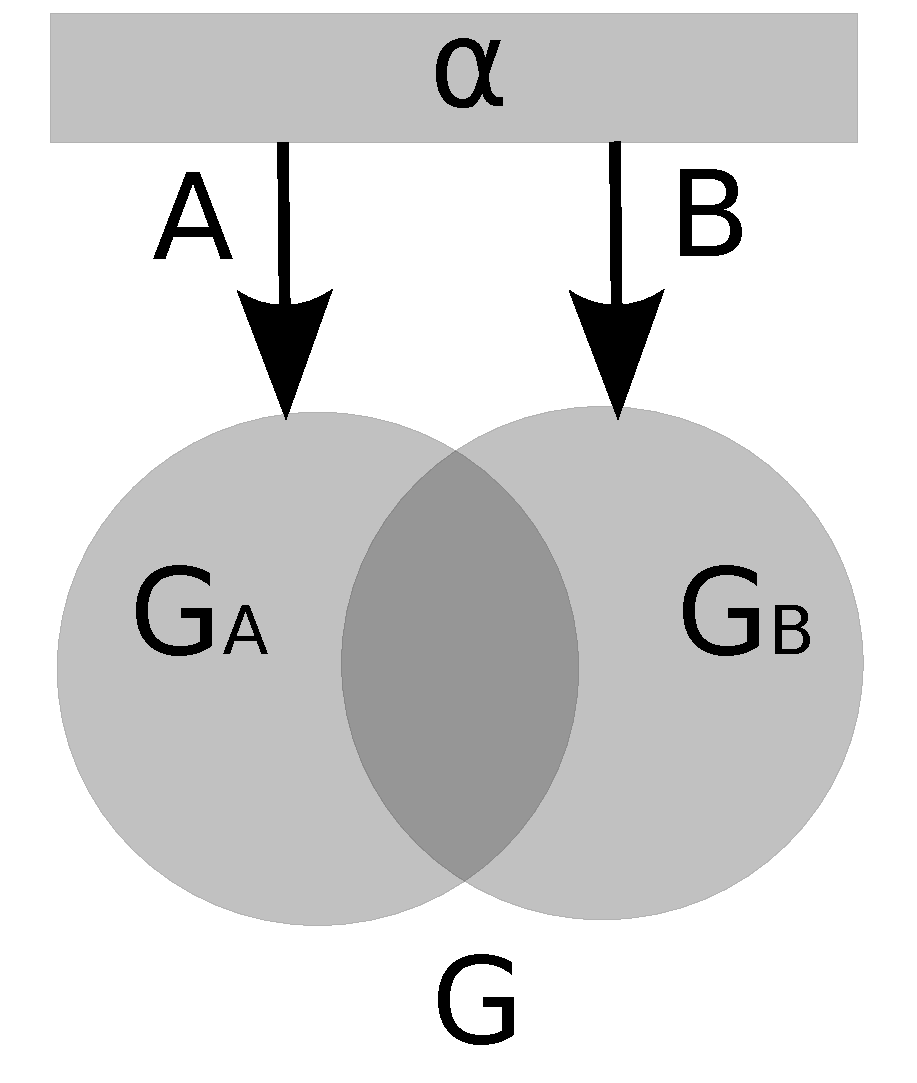
\includegraphics[height=1.18in]{figs/graphmodel2}
  %\label{fig:graph1}}
% %   \hspace{12pt}%
  \caption{Graph model}%
\label{fig:graphmodel2}
\end{minipage}
\begin{minipage}[t]{0.5\linewidth}
%\end{wrapfigure}
%\begin{wrapfigure}{r}{1.0in}
  \centering
% %   %\subfloat[Initially, the owner node $v$ publishes the object]
  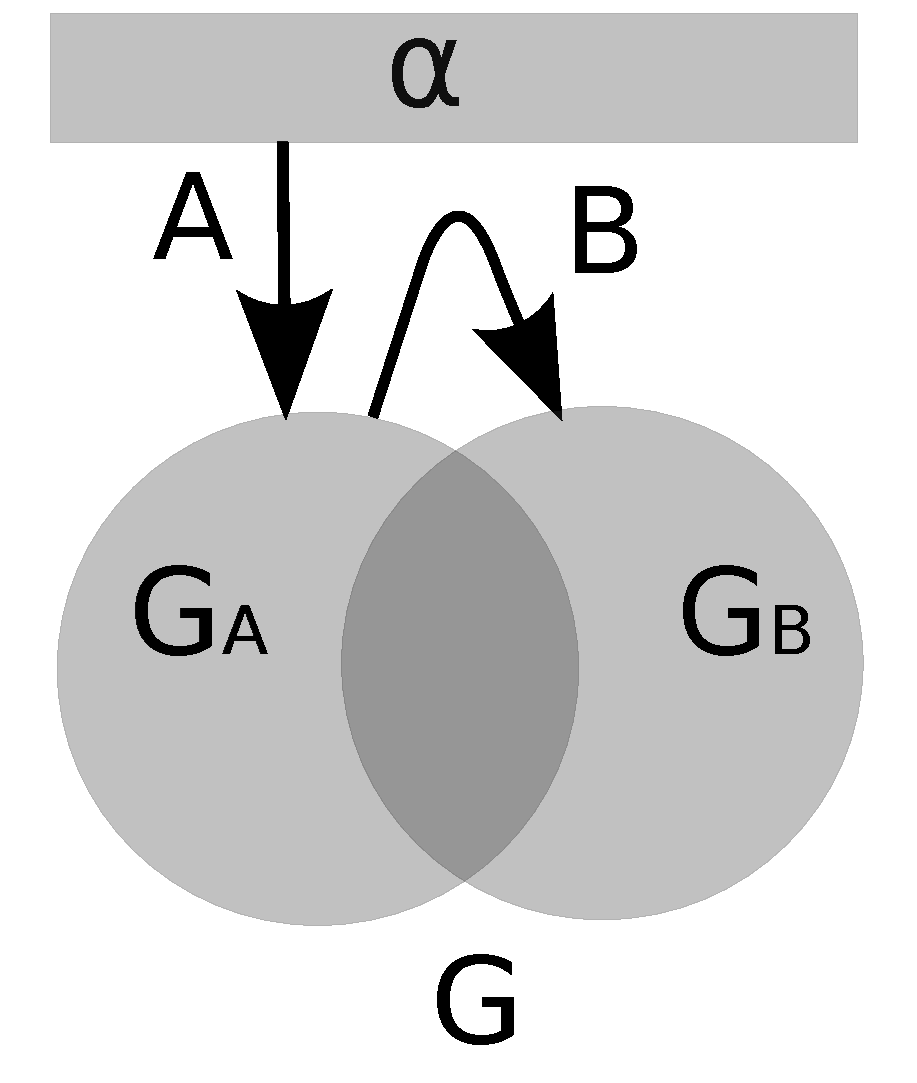
\includegraphics[height=1.18in]{figs/graphmodel2b}
  %\label{fig:graph1}}
% %   \hspace{12pt}%
  \caption{Subgraph model}%
\label{fig:graphmodel3}
\end{minipage}
\end{figure}

Our algorithm uses three phases to perform garbage collection. The three phases are $Phantomize$, $Recover$ and $CleanUp$. The $Phantomization$ phase is a kind of search that marks (i.e. phantomizes) nodes which have lost strong support. The $Recovery$ phase unmarks the nodes, reconnecting the affected subgraph to strong links. If $Recovery$ fails to rebuild links, the $CleanUp$ phase deletes them. The algorithm progresses through all three phases in the order (1. $Phantomize$, 2. $Recover$ and 3. $CleanUp$) and transitions only when there are no more operations left in the current phase. Our algorithm is concurrent because the garbage collection on different subgraphs can proceed independently until, and unless they meet.

If $G$ is the given graph and $\alpha$ is the root set prior to any deletions (see Fig.~\ref{fig:graphmodel2}), $\alpha = \{A, B\}$, and $\alpha = \{ A \}$ after deletions, then
$G$ will become $G_A$, the nodes reachable from $A$.
Thus, $G = G_A \cup G_B$  initially, and
the garbage due to the loss of  $B$ will be $\Gamma_B$.
$$\Gamma_B = G_B - (G_A \cap G_B).$$
During phantomization, all nodes in $\Gamma_B$ and some nodes in $G_A \cap G_B$ will be marked. During recovery, the nodes in $G_A \cap G_B$ will all be unmarked. Hence,
after the $Recovery$ phase, all nodes in $G_A \cap G_B$ will be strongly connected to $A$.
The final phase $CleanUp$ discards the marked memory, $\Gamma_B$.

The above discussion holds equally well if instead of being a root, $B$ is the only strong
link connecting subgraph $G_A$ to subgraph $G_B$. See Fig.~\ref{fig:graphmodel3}.

 %\subsection{Algorithm Design}


% \begin{figure}[h!]
%   \centering
% % %   %\subfloat[Initially, the owner node $v$ publishes the object]
%   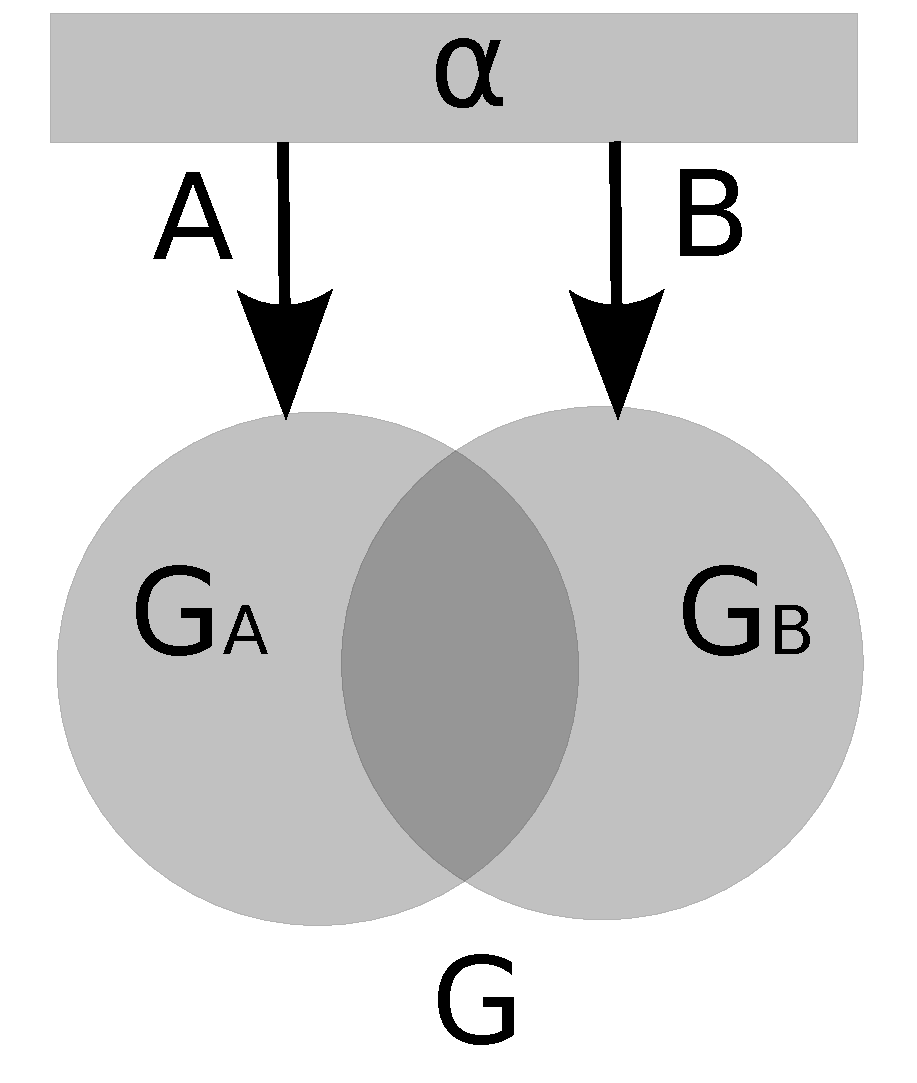
\includegraphics [height=2.5in,width=3.3in] {figs/graphmodel2}
%   %\label{fig:graph1}}
% % %   \hspace{12pt}%
%   \caption{Graph Model}%
%    \label{fig:graphmodel2}
%   \end{figure}







\begin{theorem}[Cycle Invariant]
\label{theorem:cycleinvariant}
No strong cycles are possible, and all cycles formed in the graph should have at least one weak or phantom edge in the cyclic path.
\end{theorem}
\begin{proofs}
This invariant should be maintained through out the graph for any cycles for the algorithm. This property ensures the correctness of the algorithm and the definition of the stable graph. In the rules below, the edge being created is $E$, the source node (if applicable) is called $S$, the target node is $T$. The edge creation rules state: %Assume a graph $G$ that has nodes $a_1$, $a_2$, $a_3$ ... $a_n$. If the edges formed between the nodes create a simple cycle, then by the edge creation rules,
\begin{enumerate}
\setcounter{enumi}{-1}
\item Roots always count as strong edges to nodes.
\item Edge $E$ can be strong if $S$ has no incoming strong edges from other nodes, i.e. if there is no node $C$ with a strong edge to $S$, then $E$ can be created strong. Thus, $S$ is a source of strong edges.
\item A new edge $E$ can be strong if node $T$ has no outgoing non-phantom edges, and $S \neq T$. Thus, $T$ is a terminus of strong edges.
\item A new edge $E$ is strong if $T$ is phantomized and $S$ is not. Thus, $T$ is a terminus of strong edges.
\item A new edge $E$ is weak otherwise. %only if the nodes already have a positive strong count and has outgoing edges, or if it is a self reference.
\item Edge $E$ can only be converted to strong if $T$ is phantomized.
\item A new edge $E$ must be phantom if the node $S$ is phantomized.
\end{enumerate}
Any change described by the above rules regarding strong edges results in one of the nodes becoming a source or terminus of strong edges.
Hence, no strong cycles are possible.
\end{proofs}



%Assume the nodes $a_1$, $a_2$, $a_3$...$a_n$ form a linear chain and the first node $a_1$ is supported the root $A$ in the graph $G$. As we know the nodes are created in the node listed, it was always safe to create each and every edges in the graph to be strong up until now. This makes all nodes in the graph to acquire a positive strong node which signifies the node if they are strongly reachable from any root. When the node $a_n$ creates an edges to $a_1$ to create a cycle, the edge should not be strong. The creation edge rule heuristically says that outgoing edges from the $a_1$ might transitively reach $a_n$ and create a cycle. So it is always safe to create a weak edge in this scenario. So a node with incoming weak edge is not always sign of cycle membership. So in any event, when an edges creates a cycle the edges receiver always has a outgoing edge and a positive strong count. That outgoing edge in the edge receiver should have a path to the node that closing the cycle to form a cycle. So the weak edges in the closing edge of cycle is inevitable by the rules. So thus all cycles formed in graph has at least a weak edge.
%\end{proofs}
%\begin{theorem}[termination]
%Any mutation in the graph $G$ will terminate with $G'$.
%\end{theorem}

%\begin{theorem}[termination]
%Any mutation in the graph $G$ will terminate with $G'$.
%\end{theorem}
%
%\begin{proofs}
%
%
%Assume a graph $G$ is a $Simple Cycle$ and $G$ is supported by roots $A$ and $B$. As $A$ and $B$ both can reach all the nodes in the Graph $G$
%$$G_A \equiv G_B (\because G_A \subseteq G_B)$$
%We prove the termination property by contradiction. If we assume a traversal  is non-terminating, it is only possible if the traversal does not remember the path traversed. This contradicts the marking process which  places the footprints the path traversed. So a graph cannot be traversed indefinitely if there is a mark in the visited node. If there is possibility  that concurrently marks are placed in the  graph $G$ by $A$ and $B$ is replacing the mark as it recovers, then it will indefinitely process the cycle as marking is replace by recovery (unmarking) in the graph. This also contradicts that graph does not do two different phases concurrently. So this show a graph cannot be traversed indefinitely. An action in the one phase can instantiate the action in the same phase or different phase which is eventually marking more nodes in graph or unmarking more nodes but not both at the same time. So the algorithm terminates once the affected nodes are processed. So algorithm always terminates in finite number of steps.
%\end{proofs}

\begin{theorem}[Termination]
\label{theorem:termination}
Any mutations to a stable graph $G$ will take $\cO(N)$ time steps to form a
new stable graph $G'$, where $N$ is number of edges
in the affected subgraph.
\end{theorem}

\begin{proofs}
By {\it stable graph} we mean a graph in which all nodes are strongly connected
from the roots and no phantom links or phantomized nodes are present. Mutations
which enlarge the graph, e.g. adding a root, or edge are constant time
operations since they update the counters and outgoing edge list in a node.
Mutations which diminish the graph, e.g. deleting roots, or edges potentially
begin a process of $Phantomization$, which may spread to any number of nodes in
$G$.
%The Phantomization process terminates if it fails to take away the strong link from a node, if it reaches a node which is already phantomized, or if it reaches a node with no outgoing links. Hence, the Phantomization process cannot take more steps than there are nodes and edges in the affected subgraph graph, and can only traverse a link once.

%Once the Phantomization process begins, the Recovery process begins. The Recovery process traverses each node that lost its last strong link during Phantomization and, if successful, spreads through its outgoing links. It terminates if it reaches an object that already has a strong count greater than zero. Like Phantomization, the process can, at most, spread to all nodes and follow all links in the Phantomized subgraph, and can only traverse a link once.


To prove the algorithm is linear we have to prove that each of the three phases in
the algorithm is linear in time. Without loss of generality, consider the graph
in Fig.~\ref{fig:graphmodel2} (or, equivalently, Fig.~\ref{fig:graphmodel3}). In this graph there are two sets of root links
$A$ and $B$ leading into graph $G$. The graph has three components $G_A$, $G_B$,
$G_A \cap G_B$. So,
$$G_A \cap G_B \subset G_A$$ and
$$G_A \cap G_B \subset G_B,$$
where $\pi_A$ and $\pi_B$ are only reachable  by $A$ and $B$, such that
$$\pi_A = G_A - G_A \cap G_B,$$
$$\pi_B = G_B - G_A \cap G_B.$$
$Phantomization$ starts when a node attempts to convert its weak links to
strong, and marks a path along which strong links are lost. $Phantomization$
stops when no additional nodes in the affected subgraph lose strong
support. In Fig.~\ref{fig:graphmodel2} (or Fig.~\ref{fig:graphmodel3}), the marking process will touch at least
$\pi_B$, and at most, all of $G_B$. The marking step affects both nodes and
edges in $G_B$ and ensures that graph is not traversed twice. Thus, $Phantomization$
will take at most $\cO(N)$ steps to complete where
$N$ is the number of edges in $G_B$.

$Recovery$ traverses all nodes in $G_B$ identified during
$Phantomization$. If the node is marked and has a strong count, it unmarks
the node and rebuilds its outgoing edges, making them strong or weak according to
the rules above. The nodes reached by outgoing links are, in turn,
$Recovered$ as well. Since $Recovery$ involves the unmarking of nodes, it is
attempted for every node and edge identified during phantomization, and can
happen only once, and can take at most $\cO(N)$ steps to complete.

Once the $Recovery$ operations are over, then $CleanUp$ traverses the nodes in
the recovery list. For each node that is still marked as phantomized, the node's
outgoing links are deleted. At the end of this process, all remaining nodes will
have zero references and can be deleted. Because this operation is a single
traversal of the remaining list, it too is manifestly linear.
\end{proofs}

\begin{theorem}[Safety]
Every node collected by our algorithm is indeed garbage and no nodes reachable by roots are collected.
\label{theorem:safety}
\end{theorem}
\begin{proofs}
\begin{comment}
{\color{green}
We say that a garbage collection algorithm is $safe$ if every object collected
is indeed garbage. That is, an object being cleaned up should not be reachable
from any roots.

A node is said to be prematurely deleted if the node is still reachable from some
root. So in order to prove the safety, the algorithm should prove it never
prematurely deletes a node that is reachable at any point in time.

We prove the safety by contradiction. Assume that graph $G$ at time $t$ is
stable. Assume that at time $t' > t$, an edge is removed from the set such that
node $V$ will be prematurely deleted. This means that $V$ must lose all its
strong links. The result must be that it has weak or phantom incoming links, otherwise
it should be deleted. If it has weak or phantom links, however, $V$ will
be phantomized.

If, at the conclusion of the $Phantomization$, $V$ has any non-phantom
references, then at least one will be strong, and $V$ will not collected. This contradicts our
assumption, therefore, $V$ must
only have phantom links at the end of $Phantomization.$

During the $Recovery$ phase, each phantomized node is checked for the presence of
weak or strong links and recovered if it is. If any are present, the phantom links
on $V$ will be rebuilt. Therefore, $V$ must be part of
a set of nodes which only contain phantom links. If this is so, then there can be
no root links connected to any of the objects in the set, and the whole set must
be garbage. This contradicts our assumption that $V$ was prematurely deleted.

Consider now the scenario where just after $Phantomization$ and just before $Recovery$, an edge is removed
from $V$, and just after an attempt to recover $V$ the edge is re-established.
In this case, if the live system attempts to remove a strong edge after $Phantomization$, the
edge is instead transferred to the collector thread allowing the collector thread
to handle the request at a later time. See Algorithm~\ref{algorithm:addtocollector}.
}
\end{comment}
Garbage is defined as a graph not connected to any roots. If the garbage graph contains
no cycles, then it must have at least one node with all zero reference counts. However,
at the point it reached all zero reference counts, the node would have been collected, leaving
a smaller acyclic garbage graph. Because the smaller garbage graph is also acyclic, it must lose
yet another node. So acyclic graphs will be collected.

If a garbage graph contains cycles, it cannot contain strong cycles by
Theorem~\ref{theorem:cycleinvariant}. Thus, there must be a first node in the
chain of strong links. However, at the point where a node lost its last strong
link, it would have either been collected or phantomized, and so it can not
endure. Since there no first link in the chain of strong links can endure, no
chain of strong links can endure in a garbage graph. Likewise, any node having only weak incoming
links will phantomize. Thus, all nodes in a garbage graph containing cycles
must eventually be phantomized.

If such a state is realized, $Recovery$ will occur and fail, and $Cleanup$
will delete the garbage graph.

Alternatively, we show that an object reachable from the roots will not be collected.
Suppose $V^C$ is a node and there is an acyclic chain of nodes
$ Root \rightarrow ... \rightarrow V^A \rightarrow V^B \rightarrow ... \rightarrow V^C$.
Let $V^A$ be a node that is reachable from a root, either directly or by some chain of references.
If one of the nodes in the chain, $V^B$, is connected to $V^A$
and supported only by weak references, then
at the moment $V^B$ lost its last strong link it would have phantomized and converted any
incoming weak link from $V^B$ to strong. If $V^B$ was connected by a phantom link from $V^A$,
then $V^B$ is on the recovery list and will be rebuilt in $Recovery$. This logic can be
repeated for nodes from $V^B$ onwards, and so $V^C$ will eventually be reconnected by
strong links, and will not be deleted.
\label{safety}
\end{proofs}

\begin{theorem}[Liveness]
\label{theorem:liveness}
For a graph of finite size, our algorithm eventually collects all unreachable nodes.
\end{theorem}
\begin{proofs}
We say that a garbage collection algorithm is $live$ if it eventually collects
$all$ unreachable objects, i.e. all unreachable objects are collected and never
left in the memory.
\begin{comment}
Assume that object $V$ becomes garbage but is not collected. If at any time, the
strong, weak, and phantom count on $V$ are all zero, it will be collected.
%Therefore, by the logic used in Theorem~\ref{theorem:safety}, all $V$'s incoming links must become phantomized. If it is phantomized, it
Therefore it has links. However, it must have lost its last strong link, and failed to gain a new one by phantomizing, or it is not garbage.
Therefore, it must be phantomized, and all its incoming edges must be phantoms.
If it is phantomized, it will be tested during $Recovery.$ Since
$V$ is garbage by assumption, recovery must fail. Since it was not
recovered during $Recovery$, it must be part of a set of nodes with
all phantom links. However, it is equally true that if a $Recovery$ is
attempted, a $CleanUp$ will also be attempted and $V$ will be deleted. This
contradicts our assumption that $V$ will not be deleted by our garbage collector after becoming
unreachable in a finite number of steps.
\end{comment}

The only stable state for the graph in our garbage collection is one in which all nodes
are connected by strong links, because any time the last strong link is lost a chain of
events is initiated which either recovers the links or deletes the garbage. Deletion of
a last strong link can result in immediate collection or $Phantomization.$ Once $Phantomization$
begins, it will proceed to completion and be followed $Recovery$ and $Cleanup.$ These
operations will either delete garbage, or rebuild the strong links. See Theorem~\ref{theorem:safety}.
%\end{comment}
\end{proofs}

Note that the live system may create objects faster than the
$Phantomization$ phase can process. In this case, the $Phantomization$ phase will
not terminate.
However, in Theorem \ref{theorem:liveness} when we say the graph be ``of finite size'' we
also count nodes that are unreachable but as yet uncollected,
which enables us to bound the number of nodes that are being added while the $Phantomization$ is in progress.
%, and it is for this
%objection, and similar objections, that we added the qualification that the
%graph be of finite size.
On a practical level, it is possible for garbage to be
created too rapidly to process and the application could terminate with an out-of-memory error.

\section{Experimental Results}
\label{section:experimental}
To verify our work, we modeled the graph problem described by our garbage
collector in Java using fine-grained locks. Our implementation simulates the mutator and collector
behavior that would occur in a production environment. Our mutator threads create, modify, and
delete edges and nodes, and the collector threads react as necessary. This prototype
shows how a real system should behave, and how it scales up with threads.

We also developed various test cases to verify the correctness of the garbage
collector implementation. Our test cases involve a large cycle in which the root
node is constantly moved to the next node in the chain (a ``spinning wheel''), a doubly linked list
with a root node that is constantly shifting, a clique structure, and various
tests involving a sequence of hexagonal cycles connected in a chain.

In Fig.~\ref{fig:scale} we
collected a large number of hexagonal rings in parallel. This
operation should complete in time inversely proportional to the number of threads
in use, as each ring is collected
independently. The expected behavior is observed.

In Fig.~\ref{fig:overhead} we performed the same test, but to a set
of connected rings. The collection threads
merge, but not immediately, so the collection time goes down with the number of
threads used, but not proportionally because the
collection threads only operate in parallel part of the time.

In Fig.~\ref{fig:linearity}, we perform tests to see whether our garbage
collector is linear. We considered a clique, two different hexagonal cycles (one
is interlinked and other separate), a doubly-linked list, and simple cycles, and
measured the collection time per object by varying the size of the graph and
fixing the collector threads to two all times. The results confirmed that our
collector in indeed linear in time.

Our tests are performed on two 2.6 GHz 8-Core Sandy Bridge Xeon Processors (i.e.
on 16 cores) running Redhat Linux 6 64-bit operating system.

\begin{figure}[h!]
  \centering
% %   %\subfloat[Initially, the owner node $v$ publishes the object]
  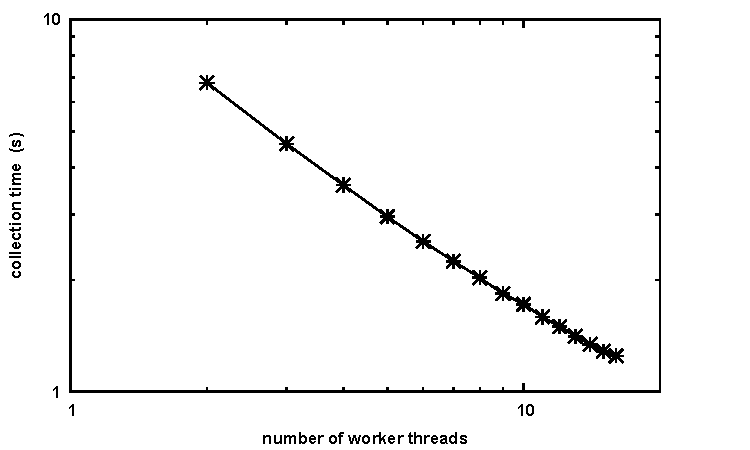
\includegraphics[height=1.8in,width=3.0in]{figs/CleanupTimeperObjectonly16log}
  %\label{fig:graph1}}
% %   \hspace{12pt}%
  \caption{
  A large number of independent rings are collected by various number of
  worker threads. Collection speed drops linearly with the number of
  cores used.
  }
   \label{fig:scale}
  \end{figure}

% % While the algorithm can scale very well with the independent sets, the collector threads working on the shared structure needs synchronization. The testcase that we used for scaling is changed so that all benzene structures are interlinked and collector has to communicate and coordinate their activities based on other collector threads. The algorithm systematically achieves optimized communication and coordination among the multiple collector threads working on the same shared structure. As a result of this, the Fig \ref{fig:overhead} shows the synchronization issues due to multiple threads interacting among each other to cleanup the structure.
\begin{figure}[h!]
  \centering
% %   %\subfloat[Initially, the owner node $v$ publishes the object]
  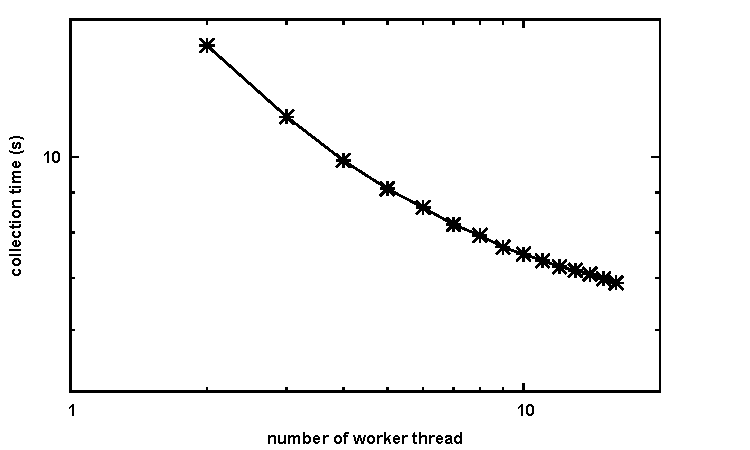
\includegraphics[height=1.8in,width=3.0in]{figs/collapseoverheadonly16log}
  %\label{fig:graph1}}
% %   \hspace{12pt}%
  \caption{A chain of linked cycles is created in memory. The connections are severed,
  then the roots are removed. Multiple collector threads are created and operations
  partially overlap.}
   \label{fig:overhead}
  \end{figure}


\begin{figure}[h!]
  \centering
% %   %\subfloat[Initially, the owner node $v$ publishes the object]
  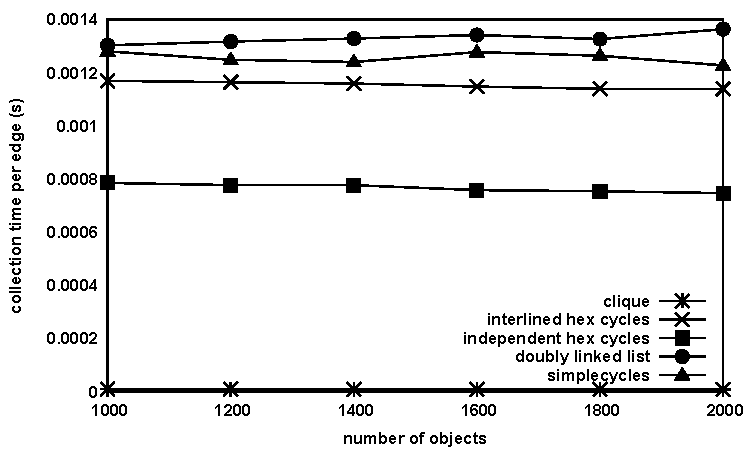
\includegraphics[height=1.8in,width=3.0in]{figs/linearity}
  %\label{fig:graph1}}
% %   \hspace{12pt}%
  \caption{
  Graphs of different types are created at various sizes in memory,
  including cliques, chains of cycles, large cycles, and large doubly
  linked lists. Regardless of the type of object, collection time
  per object remains constant, verifying the linearity of the underlying
  collection mechanism.
  }
   \label{fig:linearity}
  \end{figure}

\section{Future Work}
\label{section:future-work}
There are numerous avenues to explore within this modified Brownbridge framework.

First there are the details of the concurrent operation. While we have explored
the use of merging collector threads upon phantomization, we have not
made use of parallelism within a single collection thread's operations.
Doing so may or may not be desirable, depending on the requirements
for liveness and the compute needs of the application.

Our implementation uses fine-grained locking, but an approach using atomic
variables or atomic transactions should be possible.

Because the situations that lead to nontrivial work are algorithmic, it
should be possible for compilers to optimize instructions to create or
remove links to avoid work. Likewise, it should be possible to build
profiling tools that identify garbage collection
hot spots within a program, and give the programmer the option to take
steps (e.g. re-arrange link structure) to minimize the garbage collector's work.

We also intend to build a high performance distributed version in C++, for
use in High Performance Computing (HPC) systems.
HPC is entering a new phase  in which more complex
simulations are being carried out, covering multiple orders of time and space resolution, and
merging the time evolution of multiple kinds of calculations within a single
calculation. Parallelization of such systems is nontrivial, and increasingly
researchers are moving to dynamic parallelism managed by task queues and
active messages. Numerous frameworks exist,
or are being constructed for this purpose (Charm++~\cite{kale1993charm++},
HPX~\cite{kaiser2009parallex}, Swarm/ETI~\cite{lauderdale2012towards},
UNITAH~\cite{berzins2010uintah}, The Global Arrays
Toolkit~\cite{nieplocha1994global}, etc.)

Until this point, these systems have either required programmers to manage
memory themselves, or use a form of simple reference counting. None of the systems
above offer
an option for global garbage collection capable of reclaiming cycles. Because
garbage collection tends to be a complex, global operation which traces links
throughout memory, it has not been
considered viable in high performance computing to date. However, if the trend
toward increasingly complex multi-scale multi-physics simulations continues, it
may only be a time before garbage collection becomes a requirement.

%The High Performance ParalleX (HPX) effort is
%investigating support for garbage collection in a high performance
%computing context, and the work presented here
%provides a significant milestone in the march toward a future high performance
%implementation. It provides a concurrent implementation where most operations
%are local in nature. Collection operations, even when they contain cycles, are treated
%by operations local to a subgraph and synchronization is only required when
%these subgraphs collide.

%Because the algorithm is intrusive, that
%is because objects need to have knowledge of what pointers they have, it does
%not fit seamlessly with a C++ framework.

%Because of its novel properties, we speculate that this garbage collection
%algorithm might be useful in real time systems. While this effort would not
%be related to our core mission to improve supercomputing, it may nevertheless
%be a worthwhile avenue of study.

%In addition, we hope to discover improvements to the algorithm itself. We hope
%to find a means to minimize or remove the need for a global barrier. At very
%high computer node counts, such barriers may prove to be a significant obstacle.
%We also hope to find a means to make the system fault tolerant, another
%desirable property for computations at large scale.

\section{Conclusion}
\label{section:conclusion}
We have described a garbage collector based on strong and weak reference counts,
proven its validity,
and illustrated its potential advantages over existing systems, including:
\begin{enumerate}
\item It can run at the same time as a live system, using multiple threads if that
is desired, without needing to ``stop the world.''
%It thus may prove useful in soft real-time systems;
\item It has a reduced need to operate on memory compared to collectors because
it only performs nontrivial work when the last strong link is removed;
\item It has a reduced need to trace links in performing its operations, specifically:
\begin{enumerate}
\item When objects do not need to be collected, it is often able to prove this
without completely tracing cycles to which they belong which have support;
\item It remembers stable paths through memory and thus avoids doing work on old objects,
a benefit similar to that derived from generational collectors, e.g. \cite{Printezis:2000};
deletions are occurring;
\item When objects do need to be collected, the collector only needs to trace the cycle twice;
\item The collector operation is local;
\item The collector does not need or use back-pointers;
\end{enumerate}
These advantages should make our collector useful for distributed systems, where traces that
cross node boundaries are likely to be extremely expensive.
\end{enumerate}

Disadvantages include:
\begin{enumerate}
\item An increased memory overhead: three counters and a pointer are required
for each object;
\item An additional cost of pointer creation/mutation;
\item The lack of a fault tolerance protocol;
\item Little effort has, as yet, been devoted to optimization of any implementation. Further reduction of memory and computational overheads may yet be achieved with variations on this algorithm.
%\item The order of deletion in the $CleanUp$ phase is not, at present, guaranteed. This is a potential problem for systems in which finalizers need to run in a certain order, but a system for mitigating this issue is known to us and will be addressed in a future work.
\end{enumerate}

While there are undoubtedly cases for which the increased overheads are unacceptable,
there are just as undoubtedly cases where the potential performance gains make it acceptable.

For distributed applications, a fault tolerance protocol may be of high importance, depending
especially on the reliability of the application components. We expect, however, that variants
of this protocol and synchronization strategies associated with it may be discovered to assist
with these problems.

In short, we feel that collectors based on a system of strong and weak references like
the one we have described here have many potential advantages over existing systems and
should provide a fertile ground for future research and language development.

\section{Appendix}
\subsection{Multi-Threaded Collector}
\label{singlethread}
Note that in the following sections, locks are always obtained in canonical order that avoids deadlocks. Unlock methods unlock the last set of items that were locked.

The lists on the collectors are thread-safe.

The collector object is itself managed by a simple reference count. Code for incrementing and decrementing this count is not explicitly present in the code below.

A reference implementation is also provided ~\cite{url:refimpl}.

\begin{algorithm}[ht]
{\small
\tcp{LinkSet creates a new link,
  and decides the type of the link to create.}
{\bf LinkSet(link,node)}:\\
\quad {lock (link.Source,node)}\\
\quad {\bf if} node == NULL {\bf then}\\
\quad \quad LinkFree(link)\\
\quad \quad link.Target = NULL\\
\quad {\bf EndIf}\\
\quad {\bf if} link.Target == node {\bf then}\\
\quad \quad {\bf Return}\\
\quad {\bf EndIf}\\
\quad oldLink = copy(link) \\
\quad link.Target = node\\
\quad {\bf If} link.Source.Phantomized {\bf then}\\
\quad \quad MergeCollectors(link.Source, link.Target)\\
\quad \quad link.PhantomCount++\\
\quad \quad link.Phantomized = True\\
\quad {\bf ElseIf} link.Source == node {\bf then}\\
\quad \quad link.Which = 1 - node.Which\\
\quad \quad node.Count[link.Which]++\\
\quad {\bf ElseIf} node.Links not initialized {\bf then}\\
\quad \quad node.Count[link.Which]++\\
\quad \quad link.Which = node.Which\\
\quad {\bf Else}\\
\quad \quad link.which = 1 - node.Which\\
\quad \quad node.Count[link.Which]++\\
\quad {\bf EndIf}\\
\quad {\bf If} oldLink != NULL\\
\quad \quad LinkFree(oldLink)\\
\quad  {unlock()}\\
}
\caption{LinkSet}
\label{single:algorithm:linkset}
\end{algorithm}
\setlength{\textfloatsep}{0pt}
\begin{algorithm}[ht]
{\small
\tcp{Freeing a link is usually just the decrement of a reference count, but
if it is the last strong count, this could potentially start a Phantomization process.}
%\begin{multicols}{2}
% \tcp{$R$ and $S$ are objects currently in use.}
{\bf LinkFree(link)}:\\
% \tcp*[f]{Create a pointer from object $R$ to some free object}\\
{\Indp
{lock(link.Source,link.Target)}\\
{\bf If} link.Target == NULL {\bf then}\\
\quad {\bf Return}\\
{\bf EndIf}\\
{\bf If} link.Phantomized {\bf then}\\
\quad DecPhantom(link.Target)\\
{\bf Else}\\
\quad link.Target.Count[link.Which]-\,-\\
\quad {\bf If} link.Target.Count[link.Which] == 0 {\bf And} \\
\quad \quad \quad link.Target.Which == link.Which {\bf then}\\
\quad \quad {\bf If} link.Target.Count[1-link.Target.Which] == 0 {\bf And} \\
\quad \quad \quad \quad link.Target.PhantomCount == 0 {\bf then}\\
\quad \quad \quad Delete(node)\\
\quad \quad \quad link.Target = NULL\\
\quad \quad {\bf Else} \\
\quad \quad \quad {\bf If} link.Target.Collector == NULL {\bf then}\\
\quad \quad \quad \quad link.Target.Collector = new Collector()\\
\quad \quad \quad {\bf EndIf}\\
\quad \quad \quad AddToCollector(link.Target)\\
\quad \quad {\bf EndIf} \\
\quad {\bf EndIf}\\
{\bf EndIf}\\
{unlock()}\\
}
}
\caption{LinkFree}
\label{algorithm:linkfree}
\end{algorithm}
\setlength{\textfloatsep}{0pt}
\begin{algorithm}[ht]
{\small
%\begin{multicols}{2}
% \tcp{$R$ and $S$ are objects currently in use.}
% \tcp*[f]{Create a pointer from object $R$ to some free object}\\
\tcp{Adding an object to the collector puts back the strong
count, effectively transferring the source of the strong link
to the collector. It also adds a phantom count, which helps
prevent the clearing of the Collector field.}
{\bf AddToCollector(node)}:\\
{\Indp
{\bf While} True\\
\quad {lock(node,node.Collector)}\\
\quad {\bf If} node.Collector.Forward != NULL {\bf then}\\
\quad \quad node.Collector = node.Collector.Forward\\
\quad {\bf Else}\\
\quad \quad node.Count[node.Which]++\\
\quad \quad node.PhantomCount++\\
\quad \quad node.Collector.CollectionList.append(node)\\
\quad \quad {\bf Break}\\
\quad {\bf EndIf}\\
\quad {unlock()}\\
{\bf EndWhile}\\
}
}
\caption{AddToCollector}
\label{single:algorithm:addtocollector}
\end{algorithm}
%\end{multicols}
\setlength{\textfloatsep}{0pt}
\begin{algorithm}[ht]
{\small
%\begin{multicols}{2}
\tcp{The collector takes away the strong link it made in
AddToCollector().
}
{\bf PhantomizeNode(node,collector)}:\\
{\Indp
{lock(node)}\\
{\bf While} collector.Forward != NULL\\
\quad collector = collector.Forward\\
{\bf EndWhile}\\
node.Collector = collector\\
node.Count[node.Which]-\,-\\
\quad // Prevent deletion while the\\
\quad // node is managed by the Collector\\
{\bf Let} phantomize = False\\
{\bf If} node.Count[node.Which] $>$ 0 {\bf then}\\
\quad {\bf Return}\\
{\bf Else}\\
\quad {\bf If} node.Count[1-node.Which] $>$ 0 {\bf then}\\
\quad \quad node.Which = 1-node.Which\\
\quad {\bf EndIf}\\
\quad {\bf If} {\bf Not} node.Phantomized {\bf then}\\
\quad \quad node.Phantomized = True\\
\quad \quad node.PhantomizationComplete = False\\
\quad \quad phantomize = True\\
\quad {\bf EndIf}\\

{\bf EndIf}\\
{\bf Let} links = NULL \\
{\bf If} phantomize {\bf then}\\
\quad links = copy(node.Links)\\
{\bf EndIf}\\
{unlock()}\\
{\bf ForEach} outgoing link in links\\
\quad PhantomizeLink(link)\\
{\bf EndFor}\\
lock(node)\\
{node.PhantomizationComplete = True}\\
unlock()\\
}
%\end{multicols}
}
\caption{PhantomizeNode}
\label{algorithm:phantomizenode}
\end{algorithm}
\setlength{\textfloatsep}{0pt}
\begin{algorithm}[ht]
{\small
%\begin{multicols}{2}
\tcp{This method describes the
work to be carried out by a
garbage collection thread. Live
objects pointing to this collector, or
Forward pointers from other collectors
contribute to the RefCount field on
the Collector.}
{\bf Collector.Main()}:\\
{\Indp
{\bf While} True \\
\quad WaitFor(Collector.RefCount == 0 {\bf Or} Work to do)\\
\quad {\bf If} Collector.RefCount == 0 {\bf And} No work to do {\bf then}\\
\quad \quad {\bf Break}\\
\quad {\bf EndIf}\\
\quad {\bf While} Collector.MergedList.size() $>$ 0\\
\quad \quad Let node = Collector.MergedList.pop()\\
\quad \quad Collector.RecoveryList.append(node)\\
\quad {\bf EndWhile}\\
\quad {\bf While} Collector.CollectionList.size() $>$ 0\\
\quad \quad Let node = Collector.CollectionList.pop()\\
\quad \quad PhantomizeNode(node,Collector)\\
\quad \quad Collector.RecoveryList.append(node)\\
\quad {\bf EndWhile}\\
\quad {\bf While} Collector.RecoveryList.size() $>$ 0\\
\quad \quad Let node = Collector.RecoveryList.pop()\\
\quad \quad RecoverNode(node)\\
\quad \quad Collector.CleanList.append(node)\\
\quad {\bf EndWhile}\\
\quad {\bf While} Collector.RebuildList.size() $>$ 0\\
\quad \quad Let node = Collector.RebuildList.pop()\\
\quad \quad RecoverNode(node)\\
\quad {\bf EndWhile}\\
\quad {\bf While} Collector.CleanList.size() $>$ 0\\
\quad \quad Let node = Collector.CleanList.pop()\\
\quad \quad CleanNode(node)\\
\quad {\bf EndWhile}\\
{\bf EndWhile}\\
}
}
\caption{Collector.Main}
\label{algorithm:main}
\end{algorithm}
\setlength{\textfloatsep}{0pt}
\begin{algorithm}[ht]
{\small
%\begin{multicols}{2}
{\bf PhantomizeLink(link)}:\\
{\Indp
 {lock(link.Source,link.Target)}\\
 {\bf If} link.Target == NULL {\bf then}\\
\quad  {unlock()}\\
 \quad {\bf Return}\\
 {\bf EndIf}\\
{\bf If} link.Phantomized {\bf then}\\
\quad  {unlock()}\\
\quad {\bf Return} \\
{\bf EndIf}\\
link.Target.PhantomCount++\\
link.Phantomized = True\\
linkFree(link)\\
MergeCollectors(link.Source, link.Target)\\
 {unlock()}\\
}
}
\caption{PhantomizeLink}
\label{single:algorithm:phantomizelink}
\end{algorithm}
\setlength{\textfloatsep}{0pt}
\begin{algorithm}[ht]
{\small
%\begin{multicols}{2}
\tcp{DecPhantom is responsible for removing any reference to
the collector.}
{\bf DecPhantom(node)}:\\
{\Indp
 {lock(node)}\\
node.PhantomCount- -\\
{\bf If} node.PhantomCount == 0 {\bf then}\\
\quad {\bf If} node.Count[node.Which]== 0 {\bf And}\\
\quad \quad \quad node.Count[1-node.Which] == 0 {\bf then}\\
\quad \quad Delete(node)\\
\quad {\bf Else}\\
\quad \quad node.Collector = NULL\\
\quad {\bf EndIf}\\
{\bf EndIf}\\
 {unlock()}\\
}
}
\caption{DecPhantom}
\label{single:algorithm:decPhantom}
\end{algorithm}
\setlength{\textfloatsep}{0pt}

\begin{algorithm}[ht]
{\small
%\begin{multicols}{2}
{\bf RecoverNode(node)}:\\
{\Indp
 {lock(node)}\\
{\bf Let} links = NULL\\
{\bf If} node.Count[node.Which] $>$ 0 {\bf then}\\
\quad WaitFor(node.PhantomizationComplete == True)\\
\quad node.Phantomized = False\\
\quad links = copy(node.Links)\\
{\bf EndIf}\\
 {unlock()}\\
{\bf ForEach} link in links \\
\quad Rebuild(link)\\
{\bf EndFor}\\
}
}
\caption{RecoverNode}
\label{algorithm:recover}
\end{algorithm}
\setlength{\textfloatsep}{0pt}

\begin{algorithm}[ht]
{\small
%\begin{multicols}{2}
{\bf Rebuild(link)}:\\
{\Indp
 {lock(link.Source,link.Target)}\\
{\bf If} link.Phantomized {\bf then}\\
\quad {\bf If} link.Target == link.Source {\bf then}\\
\quad \quad link.Which = 1- link.Target.Which\\
\quad {\bf ElseIf} link.Target.Phantomized {\bf then} \\
\quad \quad link.Which = link.Target.Which\\
\quad {\bf ElseIf} count(link.Target.Links) == 0 {\bf then}\\
\quad \quad link.Which = link.Target.Which\\
\quad {\bf Else}\\
\quad \quad link.Which = 1-link.Target.Which\\
\quad {\bf EndIf}\\
\quad link.Target.Count[link.Which]++\\
\quad link.Target.PhantomCount- -\\
\quad{\bf If} link.Target.PhantomCount == 0 {\bf then}\\
\quad \quad link.Target.Collector = NULL\\
\quad {\bf EndIf}\\
\quad link.Phantomized = False \\
\quad Add link.Target to Collector.RecoveryList\\
{\bf EndIf}\\
 {unlock()}\\
}
}
\caption{Rebuild}
\label{single:algorithm:rebuild}
\end{algorithm}
\setlength{\textfloatsep}{0pt}

\begin{algorithm}[ht]
{\small
%\begin{multicols}{2}
\tcp{After deleting all the outgoing links, decrement
the phantom count by one (i.e. the reference held by
the collector itself). When the last phantom count
is gone, the object is cleaned up.}
{\bf  CleanNode(node)}:\\
{\Indp
 {lock(node)}\\
{\bf Let} die = False\\
{\bf If} node.Count[node.Which]== 0 {\bf And}\\
\quad \quad node.Count[1-node.Which]== 0 {\bf then}\\
\quad  die = True\\
{\bf EndIf}\\
{unlock()}\\
{\bf If} die {\bf then}\\
\quad {\bf ForEach} link in node\\
\quad \quad LinkFree(link)\\
\quad {\bf EndFor}\\
{\bf EndIf}\\
DecPhantom(node)\\
 }
}
\caption{CleanNode}
\label{algorithm:cleanup}
\end{algorithm}
\setlength{\textfloatsep}{0pt}
\begin{algorithm}[ht]
{\small
{\bf  Delete(node)}:\\
{\Indp
\quad {\bf ForEach} link in node \\
\quad \quad LinkFree(link)\\
\quad {\bf EndFor}\\
\quad freeMem(node)\\

 }
}
\caption{Delete}
\label{algorithm:Delete}
\end{algorithm}
\setlength{\textfloatsep}{0pt}

\begin{algorithm}[ht]
{\small
%\begin{multicols}{2}
\tcp{When two collector threads
realize they are managing a common
subset of objects, one defers to
the other. The arguments, source and
target, are both nodes.}
{\bf MergeCollectors(source,target)}:\\
{\Indp
{\bf Let} s = source.Collector\\
{\bf Let} t = target.Collector\\
{\bf Let} done = False\\
{\bf If} s == NULL {\bf And} t != NULL {\bf then}\\
\quad lock(source)\\
\quad source.Collector = t\\
\quad unlock()\\
\quad {\bf Return}\\
{\bf EndIf}\\
{\bf If} s != NULL {\bf And} t == NULL {\bf then}\\
\quad lock(target)\\
\quad target.Collector = s\\
\quad unlock()\\
\quad {\bf Return}\\
{\bf EndIf}\\
{\bf If} s == NULL {\bf Or} s == NULL {\bf then}\\
\quad {\bf Return}\\
{\bf EndIf}\\
{\bf While Not} done\\
\quad  {lock(s,t,target,source)}\\
\quad {\bf If} s.Forward == t and t.Forward == NULL {\bf then}\\
\quad \quad target.Collector = s\\
\quad \quad source.Collector = s\\
\quad \quad done = True\\
\quad {\bf ElseIf} t.Forward == s and s.Forward == NULL {\bf then}\\
\quad \quad target.Collector = t\\
\quad \quad source.Collector = t\\
\quad \quad done = True\\
\quad {\bf ElseIf} t.Forward != NULL {\bf then}\\
\quad \quad t = t.Forward \\
\quad {\bf ElseIf} s.Forward != NULL {\bf then}\\
\quad \quad s = s.Forward \\
\quad {\bf Else}\\
\quad \quad Transfer s.CollectionList to t.CollectionList \\
\quad \quad Transfer s.MergedList to t.MergedList \\
\quad \quad Transfer s.RecoveryList to t.MergedList \\
\quad \quad Transfer s.RebuildList to t.RebuildList \\
\quad \quad Transfer s.CleanList to t.MergedList \\
\quad \quad target.Collector = t\\
\quad \quad source.Collector = t\\
\quad \quad done = True\\
\quad {\bf EndIf}\\
\quad unlock()\\
{\bf EndWhile} \\
}
}
\caption{MergeCollectors}
\label{algorithm:mergecollectors}
\end{algorithm}

\clearpage

\begin{comment}
\acks
%\subsection{Acknowledgements}
We acknowledge the support
of the following grants: The DoE XPRESS proposal
(DE-SC0008714), and the NSF PXGL (1160602).
We thank Frank L\"{o}ffler and Hartmut Kaiser for
helpful conversations.
%Acknowledgments withheld to facilitate double-blind
%review.


\bibliographystyle{abbrvnat}
\bibliography{paper}
%\clearpage
\appendix

%\subsection{Multi-Threaded Collector}
%\label{multithread}
%\input{algo}
\end{document}
\end{comment}
\chapter{Distributed Memory Garbage Collection}
\chapter{Distributed Memory Single Collector Garbage Collection}
  \chapter{Distributed Memory Multi-collector Garbage Collection}
     \label{distributed}
     \begin{comment}
\documentclass[11pt]{article}
\usepackage[text={6.6in,9.3in},centering]{geometry}
\usepackage{times}
\usepackage{amsthm}
%\usepackage[ruled,vlined,linesnumbered]{algorithm2e}
\usepackage{amssymb, amsmath}
\usepackage{color}
\usepackage{graphicx}
%\usepackage{subfig}
\usepackage{lipsum}
\usepackage{wrapfig}
\usepackage{url}
\usepackage{hyperref}
\usepackage{verbatim}
\usepackage{xcolor}
\usepackage{algorithm}
\usepackage{amsmath}
\usepackage{multicol}
\usepackage{algpseudocode}
\usepackage{subcaption}
\usepackage{tikz}
\usetikzlibrary{arrows}
\usepackage{cleveref}
%\usepackage{algcompatible}

 \usepackage{pstricks}
% The following commands are not supported in PSTricks at present
% We define them conditionally, so when they are implemented,
% this pstricks file will use them.
\ifx\setlinejoinmode\undefined
  \newcommand{\setlinejoinmode}[1]{}
\fi
\ifx\setlinecaps\undefined
  \newcommand{\setlinecaps}[1]{}
\fi
% This way define your own fonts mapping (for example with ifthen)
\ifx\setfont\undefined
  \newcommand{\setfont}[2]{}
\fi

\algtext*{EndIf}% Remove "end if" text

%\newtheorem{theorem}{Theorem}[section]

\newtheorem{theorem}{Theorem}
\newtheorem{lemmas}{Lemma}
\newtheorem{axioms}{Axiom}
\newtheorem{lemma}[lemmas]{Lemma}
\newtheorem{axiom}[axioms]{Axiom}
\newtheorem{claim}[theorem]{Claim}
\newtheorem{fact}[theorem]{Fact}
\newtheorem{corollary}[theorem]{Corollary}
\newtheorem{definition}{Definition}
\newtheorem{observation}[lemmas]{Corollary}
\newtheorem{invariant}{Invariant}

\newtheorem*{rep@theorem}{\rep@title}
\newcommand{\newreptheorem}[2]{%
\newenvironment{rep#1}[1]{%
 \def\rep@title{#2 \ref{##1}}%
 \begin{rep@theorem}}%
 {\end{rep@theorem}}}


\newreptheorem{theorem}{Theorem}
%\newtheorem{lemma}{Lemma}
\newreptheorem{lemma}{Lemma}



\newcommand{\sq}{\hbox{\rlap{$\sqcap$}$\sqcup$}}
%\newcommand{\qed}{\hspace*{\fill}\sq}
%\newenvironment{proof}{\noindent {\bf Proof.}\ }{\qed\par\vskip %4mm\par}
\newenvironment{proofs}{\noindent {\bf Proof (sketch).}\ }{\qed\par\vskip
0mm\par}

\newcommand{\todo}[1]{\textcolor{red}{\textsf{[#1]}}}
\newcommand{\srb}[1]{\textcolor{blue}{\textsf{Steve: [#1]}}}
\newcommand{{\rh}}{{\widehat r}}
\newcommand{{\Rh}}{{\widehat R}}
\newcommand{\E}{{\mathcal E}}
\newcommand{\T}{{\mathcal T}}
\newcommand{\ww}{{\mathfrak{w}}}
\newcommand{\diam}{{\rm diam}}
\newcommand{\dist}{{\rm dist}}
\newcommand{\length}{{\rm length}}
\newcommand{\publish}{{\sl publish}}
\newcommand{\move}{{\sl move}}
\newcommand{\lookup}{{\sl lookup}}
\newcommand{\Read}{{\rm Read}}
\newcommand{\Write}{{\rm Write}}
\newcommand{\mysf}[1]{\textup{\sffamily #1}}
\newcommand{\CONGEST}{\mysf{CONGEST}}

\newcommand{\note}[1]{[[[{\bf #1}]]]}

\newcommand\outneighbors{\mathop{\mbox{$out$-$\mathit{neighbors}$}}}
\newcommand\inneighbors{\mathop{\mbox{$in$-$\mathit{neighbors}$}}}
\newcommand\maxweight{\mathop{\mbox{$max$-$\mathit{weight}$}}}
\newcommand\nonstrong{\mathop{\mbox{$non$-$\mathit{strong}$}}}


\begin{document}
\sloppy
\begin{titlepage}

\title{Distributed Garbage Collection for General Graphs}

\author{
Hari Krishnan\thanks{Corresponding author.} \thanks{Center for Computation and Technology, and Computer
Science and Engineering Division, Louisiana State University, LA 70803.}\\
{\em  Louisiana State University}\\
\url{hkrish4@tigers.lsu.edu}
\and
Steven R Brandt\thanks{Center for Computation and Technology, and Computer
Science and Engineering Division, Louisiana State University, LA 70803.} \\
{\em  Louisiana State University}\\
\url{sbrandt@cct.lsu.edu}
\and
Costas Busch\thanks{Computer Science and Engineering Division, Louisiana State
University, LA 70803.}\\
{\em Louisiana State University}\\
\url{busch@csc.lsu.edu}
\and
Gokarna Sharma\thanks{Department of Computer Science, Kent
State University, OH 44242}\\
{\em Kent State University}\\
\url{sharma@cs.kent.edu}
}

\date{}
\maketitle


\begin{abstract}

We propose a scalable, cycle-collecting, decentralized, reference counting
garbage collector with partial tracing.  The algorithm is based on the
Brownbridge system but uses four different types of references to label edges
in the reference graph. Memory usage is $O(\log n)$ bits per node, where $n$ is the
number of nodes in the graph.  The algorithm assumes an asynchronous network
model with a reliable FIFO channel. It collects garbage in
$O(E)$ time, where $E$ is the number of edges in the induced subgraph of the reference graph. The
algorithm uses termination detection to manage the
distributed computation, a unique identifier to break the symmetry among
multiple collectors, and a transaction-based approach 
when multiple collectors conflict. Unlike existing
algorithms, ours is not centralized, does not require barriers,
does not require
migration of nodes, does not require back-pointers on every edge,
and is stable against concurrent mutation. %, even with multiple collection
%operations overlapping the induced subgraph.

%\keywords{Distributed Garbage Collection, Distributed Termination Detection,
%Strong Weak Phantom, Reference Count}
\end{abstract} 

\centerline{}
\centerline{}
\centerline{{\bf Regular Paper. Consider also for Brief Announcement.}}
\centerline{{\bf Eligible for best student paper award: Hari Krishnan is a full
time student.}}

\thispagestyle{empty}


\end{titlepage}
\end{comment}

\section{Introduction}

Garbage-collected languages are widely used in distributed systems, including big-data applications in the cloud~\cite{maas2015trash,gog2015broom}.  Languages  in this space include
Java, Scala, Python, C\#, PHP, etc., and platforms include Hadoop, Spark,
Zookeeper, DryadLINQ, etc. In addition, cloud services such as Microsoft Azure and
Google AppEngine, and companies such as Twitter and Facebook all make significant
use of garbage-collected languages in their code
infrastructure~\cite{maas2015trash}.  Garbage collection is seen as a
significant benefit by the developers of these applications and platforms
because it eliminates a large class of programming errors, which translates
into higher developer productivity.
%Unfortunately, this cost can become high
%when object references are allowed to point outside of or between single
%shared memory systems.

Garbage collection is also an issue in networked object
stores, which share many properties with distributed systems. Like
such systems, they cannot use algorithms that require scanning the entire heap.
In any situation in which traces can go across storage boundaries, i.e. from
node to node, node to disk, etc., garbage collectors that need to trace the heap
becomes impractical.  What is needed is something distributed, decentralized, scalable,
that can run without ``stopping
the world,'' and has good time and space complexity.

%We note that time complexity may be of particular interest in increasing productivity.
%Many garbage-collection system are not able to reliably inform the programmer when
%objects are ready for reclamation. Most garbage collected languages make little effort
%to call destructors, or finalizers, and so this important feature is often unusable.

%In this present work we address all concerns except the last. We note, however,
%that as machines have scaled up they have also become more reliable and failures
%are not seen as frequently as many have feared.

%Distributed systems access objects stored at remote sites. Programming
%languages access objects allocated in the heap using stack variables and
%global variable.  They are often referred as roots. In the distributed
%systems, the heaps are distributed across sites and inter-site heap references
%are allowed. Any object is considered live only when it is reachable from any
%root.  So all objects that are not reachable will never be used and called
%garbage.  Garbage collectors identify the objects that are garabge and reclaim
%them.
There are two main types of garbage collectors, namely Tracing and Reference
Counting (RC). Tracing collectors track all the reachable objects from the root (in the reference graph)
and delete all the unreachable objects.
RC collectors
count the number of objects pointing to a given block of data at any point in
time.  When a reference count is decremented and becomes zero, its object is
garbage, otherwise it {\em might} be
garbage and some tracing is necessary (note that pure RC collectors do not trace and will not collect cycles ~\cite{rcfail}).  Unfortunately, cycles among distributed objects are
frequent~\cite{richer}.
%Our algorithm belongs to the family of hybrid RC collectors, which is RC with partial tracing. It advances the use of a
%three reference count collector designed for a single machine~\cite{Brandt2014}
%based on the Brownbridge~\cite{Brownbridge1985} algorithm. The advantage for such
%systems is that they can frequently determine that a reference count decrement
%does not create garbage without the need for tracing.
Previous attempts at distributed garbage collection, e.g. \cite{Hudak:1982,Ladin,LeFessant,liskov97,liskov95,Veiga}, suffer from the need for centralization,
%cooperation among all sites,
global barriers,
the migration of objects, or have inefficient time and space complexity guarantees.
%Our algorithm can be used in a system where the migration of the objects are
%not acceptable.
%In the work that follows we first describe the operation of a serial version
%of the collector, then proceed to discussion of the parallel version.



%%Objects become unreachable. The reclaimation of these unreachable objects are
%necessary for better performance. So distributed garbage collectors are
%inevitable in distributed systems.
%Although the distributed garbage collection is an active area of research, most
%of the interesting algorithms published are not practical. They are either
%centralized, require synchronization among all sites (a global barrier), or
%require migration of all objects in one cycle to a common machine.
%an accurate summary?}

%To identify all the nodes that are dead in graph G, there are multiple
%alternatives already available. The two abstract approach can be classified into
%two ideas of same coin. The first idea is identifying all the live nodes and
%then detecting the dead nodes. This approach is generally called as tracing
%approach. Tracing approaches uses an attribute called mark which will be set if
%there collectors reaches the node from root set R transitively. Then all the
%nodes where mark is not set in the garbage detection process will be considered
%garbage and deleted. This approach makes it clear that the node will not be able
%to detect if it is a garbage. A centralized component is required to find all
%the nodes that are live and then detect dead nodes. These systems are clearly
%not scalable as they require synchronization among all collection processes. As
%the model does not allow the nodes to know the $\inneighbors$ of a node,
%traversing all the nodes backwards to detect if the node has a path from any
%root is not considered. The model reflects the practical model used by real-time
%systems, that back edges for all $\inneighbors$ creates a additional memory
%overhead for each node. The additional memory overhead to save back edges can
%bounded to O(V).

%The second technique is identifying all the dead nodes by itself. This technique
%is widely called reference counted system. The nodes count the number of the
%incoming edges. This approach can detect a set of dead nodes trivially. When
%there are no incoming edges to a node, it is clear that the node is dead. The
%challenge in the reference counted system is node can be dead even if the node
%$x$ has incoming edges. If all dead nodes has at least an incoming edge from
%other dead node, garbage goes undetectad by simple reference counter. A simple
%example would be a cycle created by dead nodes and no node in the cycle has a
%path from root to it. Although simple reference counting suffers from complete
%garbage collection, they gained popularity because of the promptness and
%traversal cost to detect garbage. An garbage collection algorithm can be called
%prompt if it can detect dead node immediately and avoid dead nodes floating
%around. If reference counting technique can collect a cycle garbage and employ
%decentralized decision using locality, these properties make it suitable for the
%distributed system as they are easily scalable and prompt. A vast literature of
%cycle collecting reference counting asynchronous shared memory garbage
%collectors are available. All cycle collecting reference counted garabge
%collectors are hybrid approach. In fair execution, to detect dead nodes, the
%system employs a traversal that visits only a subset of nodes in graph. All
%asynchronous shared memory cycle collecting reference counted garbage collectors
%require some centralized data structure to detect dead nodes in dynamic graph
%with multiple garbage detection process running simultaneously. A centralized
%data structure based distributed algorithm will have bottlenecks and cannot be
%self stabilizing. To avoid all the bottlenecks and make the distributed garbage
%collection truely decentralized, our algorithm elminates use of centralized
%approach among all garbage detection processes in the distributed system and a
%node can make a decision about its liveness in finite steps once the node is
%dead.

\paragraph{Contributions:}
We present a hybrid reference counting algorithm for garbage collection in
distributed systems that works on the asynchronous model of communication with
reliable FIFO channel. Our algorithm collects both
non-cyclic and cyclic garbage in distributed systems of arbitrary topology by advancing on the
three reference count collector which only works for a single machine~\cite{Brandt2014}
based on the Brownbridge system~\cite{Brownbridge1985} \footnote{
Note, the original algorithm of Brownbridge suffered from premature collection, and subsequent attempts to remedy this problem needed exponential time in certain scenarios \cite{Salkild1987,Pepels1988}. We addressed those limitations in \cite{Brandt2014}.
}. The advantage for such
systems is that they can frequently determine that a reference count decrement
does not create garbage without the need for tracing. 
%However, our technique in \cite{Brandt2014} does not extend directly to the distributed garbage collection scenario involving multiple sites.

Our proposed algorithm is scalable
because it collects garbage in $O(E)$ time using only $O(\log n)$ bits memory per
node, where $E$ is the number of edges in the affected subgraph (of the reference
graph) and $n$ is the number of nodes of the reference graph. Moreover, in
contrast to previous work, our algorithm does not need centralization,
global barriers, or the migration of objects. Apart from the benefits
mentioned above, our algorithm handles concurrent mutation (addition and deletion of edges and nodes in the reference graph) and provides liveness
and safety guarantees by maintaining a property called \emph{isolation}.
Theorems \ref{pro:livenesss} and \ref{pro:safetys} prove that when a
collection process works alone (i.e. in isolation), it is guaranteed to collect
garbage and not to prematurely delete. Theorem \ref{thm:alliso} proves that
when multiple collection processes interact, our synchronization mechanisms
allow each of them to act as if they were working alone, and Theorems
\ref{liveness} and \ref{safety} prove the correctness in this setting.
To the best of our knowledge, this is the first algorithm for garbage
collection in distributed systems that simultaneously achieves such guarantees.

This algorithm falls into the category of self-stabilization algorithms, because
it maintains the invariants (1) all nodes strongly connected, (2) no strong
cycles, and (3) no floating garbage.

\paragraph{Related Work:}
%All existing garbage collectors designs fall into to one of these categories:
%Tracing, Reference Count and Hybrid.
Prior work on distributed garbage collection is vast; we discuss here the papers that are closely related to our work.  %Many of these collectors
%suffer from the need for centralization, global barriers,
%the migration of objects, or have inefficient time and space complexity.
The marking algorithm proposed by Hudak~\cite{Hudak:1982} requires a global barrier.
All local garbage
collectors coordinate to start the marking phase. Once the marking phase is over
in all the sites, then the sweeping phase continues. Along with the marking and sweeping overhead,
there are consistency issues in tracing based collectors~\cite{shapiro95}.

Ladin and Liskov~\cite{Ladin} compute reachability of objects in a highly
available centralized service. This algorithm is logically centralized but
physically replicated, hence achieving high availability and fault-tolerance.
All objects and tables are backed up in stable storage. Clocks are synchronized
and message delivery delay is bounded. These assumptions enable the centralized
service to build a consistent view of the distributed system. The centralized
service registers all the inter-space references and detects garbage using a standard
tracing algorithm. This algorithm has scalability issues due to the centralized
service. A heuristic-based algorithm by Le Fessant ~\cite{LeFessant} uses the minimal number
of inter-node references from a root to identify ``garbage suspects'' and then
verifies the suspects. The algorithm propagates marks from the references to all the
reachable objects. A cycle is detected when a remote object receives only its
own mark. The algorithm needs tight coupling between local
collectors and time complexity for the collection of cycles is not analyzed.

Collecting distributed garbage cycles by backtracking is proposed by Maheshwari
and Liskov~\cite{liskov97}. This algorithm first hypothesizes that objects are dead and
then tries to backtrack and prove whether that is true. The algorithm
needs to use an additional datastructure to store all inter-site references.
An alternative approach of distributed garbage collection by
migrating objects have been proposed by Maheshwari and Liskov~\cite{liskov95}. Both
of the algorithms use heuristics to detect garbage. The former one uses more
memory, the latter one increases the overhead by moving the objects between the
sites. Recently, Veiga et al.~\cite{Veiga} proposed an algorithm that uses
asynchronous local snapshots to identify global garbage. Cycle detection
messages (CDM) traverse the reference graph and gain information about the
graph. A drawback of this approach is that the algorithm doesn't work with the $\mathcal{CONGEST}$ model. %the growth of the messages is limited
%only by the size of the distributed system.
Any change to the snapshots
has to be updated by local mutators, forcing current global garbage collection
to quit. For a thorough understanding of the literature, we recommend reading~\cite{shapiro95, Abu}.


%\subsection{Distributed Garabge Collection = GC + Distributed Termination
%Detection}
%necessary in decentralized algorithm}

%Distributed termination detection(DTD) is a fundamental to distributed
%computation. The solution can be applied to any computation that tries to
%evaluate some stable property.
%Examples of such properties are
%deadlock detection, garbage detection etc. Once a system eventually enters into
%deadlock, it remains deadlocked. Once an object becomes garbage, it remains so.
%Detecting whether the stable property is reached is equivalent to termination in
%the DTD. The DTD can be formally described as a collection of processes
%communicating by messages. A process can be either passive or active. Active
%processes may send message while passive process will not send message. A passive
%process will be become an active when a message is received. When all the
%distributed processes are passive, the stable property is achieved. Stability
%here means no messages are in flight. The popular termination detection algorithms
%are ~\cite{dijk83,Tel88,dijk80,Misra82,Chandra90,nir}. Dijkstra and Scholten
%~\cite{dijk80} create spanning trees of the graph for detecting the termination
%detection. Our algorithm uses their solution to control the traversal and detect
%the termination.

%Tel et al showed that Distributed Termiantion Detection Algorithm (DTDA) can be
%derived from Garbage Collection Schemes.~\cite{Tel:1993}. Following Tel et al,
%Blackburn et al describes that reversing mapping is also
%possible~\cite{Blackburn:2001}. They also explained
%that any known DTDA with a centralized garbage collection will produce a
%distrbuted garbage collector (DGC). Although the literature clearly
%demonstrates the relationship between the fundamental problems of DTDA and DGC, cyclic
%reference counting-based DGC algorithm that contains this relation have never
%been explored. To our knowledge this is the first article that to do so.

%Most modern programming languages use heap and stack memory to run application.
%Objects are allocated in heap memory to increase the lifetime of the object.
%Managed runtime systems help developers to ignore the efficient deallocation of
%the objects. These managed runtime systems identify the heap allocated objects
%that are garbage and deallocate them. The relationship among various allocated
%objects in memory can be modeled as directed graph. Pointers that are in stack
%can hold reference to object in the heap. These pointers are generally referred
%as roots. Also, global pointers can also be considered as roots. In abstract,
%any pointer that does not reside in heap memory but holds reference to heap
%objects are called roots. Any objects in the heap are called nodes. These nodes
%are synonymous to regular graph nodes in graph theory. Any node can hold
%reference to any other node. These references are unidirectional link incident
%on two nodes. So they form a directed graph. The distinction between roots and
%nodes are any root can hold reference to nodes but nodes can only reference to
%other nodes. To map this into graph, we have two kind of vertices. Roots are
%special vertices that does not have any incoming link but an outgoing link.
%Nodes are regular vertex that can have incoming and outgoing links. A node is
%considered reachable if the node has a path from one of the root node to it.
%Unreachable nodes are called garbage and needs to be deleted for efficiency. The
%problem of garbage collection can be described as problem of finding all the
%garbage nodes in the reference graph and reclaim/delete them.

%It is shown in ~\cite{Tel:1993,Blackburn:2001} that there is
%strong relation between DTD and distributed garabge collection. Tel et al shown
%that a distributed termination detection algorithm can be derived from any
%distributed garabge collector~\cite{Tel:1993}. Blackburn et al, described that a
%distributed garbage collector is composite of distributed termination detection
%and a garbage collector ~\cite{Blackburn:2001}. Our algorithm indeed has a
%distributed termination detection algorithm in it along with a garbage
%collection algorithm.

%\subsection{Contributions}

\paragraph{Paper Outline:}
%The rest of the paper is organized as follows.
Section \ref{model} describes the garbage collection problem, constraints involved in the problem, and the model for which the algorithm is presented. Section \ref{single} explains the single collector version of the algorithm and provides correctness, time, and space guarantees.
Section \ref{multi} extends the results of Section \ref{single} to the multiple collector scenario. Finally, Section \ref{section:conclusions} concludes the paper with a short discussion. Some of the proofs and the pseudocode for the algorithms may be found in Appendix \ref{section:appendix}.



\section{Model and Preliminaries}
\label{model}
\paragraph{Distributed System:}
We consider a distributed system of nodes
%A distributed algorithm is one where
%self-stabilization problem where nodes
%the dead nodes identify that they are dead and
%delete themselves. Identifying a dead node by itself is not trivial in most
%cases. Each node can be assumed to
where each node operates independently and communicates with other nodes through
message passing. The underlying topology of the system is assumed to be arbitrary but connected. Each node has a queue to receive messages, and in response to a message a node can only read and write its own state and send additional messages. %A node can only send a
%message to its out-neighbors and parent of the node. Parent, a chosen node in
%$\Gamma_{in}$ from communication happened by our algorithm, .
We further assume that the nodes can communicate over
a reliable FIFO channel and that messages
are never lost, duplicated, or delivered out of order.
These properties make our system compatible with the $\mathcal{CONGEST}$ asynchronous network model with no failures ~\cite{congest}.
%Each site has memory where the objects reside. \todo{need precise definition}

\paragraph{Basic Reference Graph:}
We model the relationship among various objects and pointers in memory through a directed graph $G = (V, E)$, which we call a {\it reference graph}.
The graph $G$ has a special node $R$, which we call the {\it root}. Node $R$
represents
global and stack pointer variables, and
thus does not have any incoming edges.
Each node in $G$ is assumed to contain a unique ID. % to distinguish it within
%$G$. (For example, when each node of $G$ maps to a unique site in $H$, then ID of the site in $H$ can be used for the ID of the node in $G$.)
All adjacent nodes to a given node in $G$ are called $neighbors$, and denoted by $\Gamma$. The
$\inneighbors$ of a node $x\in G$ can be defined as the set of nodes whose outgoing edges
are incident on $x$, represented by $\Gamma_{in}(x)$. The $\outneighbors$ of $x$ can be defined as the set
of nodes whose incoming edges originate on $x$, represented by $\Gamma_{out}(x)$.
Note that each node $x\in G$ does not know $\Gamma_{in}(x)$ at any point in time.
%This constraint
%reduces memory complexity, thereby making
%the algorithm more practical and scalable. \todo{remove preceding sentence?}

\paragraph{Distributed Garbage Collection Problem:}
All nodes in $G$ can be classified as either {\em live} (i.e., not garbage) or {\em dead} (i.e., garbage) based on a property called
$reachability$. Live and dead nodes can be defined as below:


%$Live(x)= \exists y \in V \mid Reachable(y, x)$

%$Reachable(y, x) = x \in R \vee (Live(y) \wedge x \in \Gamma_{out}(y))$

$Reachable(y,x) = x \in \Gamma_{\rm out}(y) \lor (x \in \Gamma_{\rm out}(z) \mid Reachable(y,z))$

$Live(x) = Reachable(R,x)$

$Dead(x) = \neg Live(x)$

%From above definition, it is clearly that all root nodes are always reachable / live.
We allow the live portion
of $G$, denoted as $G'$, to be mutated while the algorithm is running, and we refer
to the source of these mutations as the {\em Adversary.}
The Adversary can create nodes and attach them to $G'$, create new edges between existing nodes of $G'$, or delete edges from $G'$. Moreover, the Adversary can perform multiple events (creation and deletion of edges)
simultaneously. The Adversary, however, can never mutate the dead portion of the graph $G'' = G\backslash G'$.
%Creation event represents creating directed
%edges. An edge can be only created between two live nodes in $G$. To create a
%node, an edge is created between a live node and non-existing node. During link
%creation, if the node is not available, the requested node is created and a
%directed edge is incident on newly created node. So the newly
%created node is always reachable. Deletion happens only for edges. Adversary can
%delete outgoing edge of a node $x$ only if $x$ is live . So $A$ cannot perform
%any mutation on dead nodes. These constraints create the following principles /
%axioms in the model.

\begin{axiom}[Immutable Dead Node]
 The Adversary cannot mutate a dead node.
 \label{ax:immut}
\end{axiom}

\begin{axiom}[Node Creation]
 All nodes are live when they are created by the Adversary.
\end{axiom}

From Axiom \ref{ax:immut}, it follows that a node that becomes dead will never
become live again.
%This property allows the problem to be solved in
%finite time. \todo{remove preceding sentence}
%The problem of distributed garbage collection can be modeled as
%detecting all dead nodes in dynamic directed graph $G$.

Each node experiencing deletion of an incoming edge has to determine whether it is still
live. If a node detects that it is dead then it must delete itself from the
graph $G$. %The problem of garbage collection is the process of
%identifying dead nodes in $G$ and deleting them.

\begin{definition}[Distributed Garbage Collection Problem]
%The problem of garbage collection is the process of
Identify the dead nodes in the reference graph $G$ and delete them.
\end{definition}

%We consider a distributed system where
%%A distributed algorithm is one where
%%self-stabilization problem where nodes
%%the dead nodes identify that they are dead and
%%delete themselves. Identifying a dead node by itself is not trivial in most
%%cases. Each node can be assumed to
%each node communicates with other nodes through
%messages. Each node has a queue to receive messages, and in response to a message a node can only read and write its own state and send additional messages. %A node can only send a
%%message to its out-neighbors and parent of the node. Parent, a chosen node in
%%$\Gamma_{in}$ from communication happened by our algorithm, .
%We further assume that the algorithm communicates over
%a reliable FIFO channel and that messages
%are never lost, duplicated, or delivered out of order.
%These properties make this algorithm compatible with the $\mathcal{CONGEST}$~\cite{congest} asynchronous network model with no failures.  \todo{talk also about fair execution here which is currently missing}
%%The $\mathcal{CONGEST}$ model adds the additional requirement that %messages are limited in size to $O (\log N)$. This limit is %already reached if unique object ID's are present in a message, as %they are of size $O (\log N)$.

%\subsection{Preliminaries}

\begin{figure}
\centering
%\begin{center}
\scalebox{0.6}[0.6]{% Graphic for TeX using PGF
% Title: /home/hkrish/podcpaper/distgc/completeabstract.dia
% Creator: Dia v0.97.2
% CreationDate: Wed Apr 27 12:51:38 2016
% For: hkrish
% \usepackage{tikz}
% The following commands are not supported in PSTricks at present
% We define them conditionally, so when they are implemented,
% this pgf file will use them.
\ifx\du\undefined
  \newlength{\du}
\fi
\setlength{\du}{15\unitlength}
\begin{tikzpicture}
\pgftransformxscale{1.000000}
\pgftransformyscale{-1.000000}
\definecolor{dialinecolor}{rgb}{0.000000, 0.000000, 0.000000}
\pgfsetstrokecolor{dialinecolor}
\definecolor{dialinecolor}{rgb}{1.000000, 1.000000, 1.000000}
\pgfsetfillcolor{dialinecolor}
\definecolor{dialinecolor}{rgb}{1.000000, 1.000000, 1.000000}
\pgfsetfillcolor{dialinecolor}
\fill (19.500000\du,13.250000\du)--(19.500000\du,15.150000\du)--(21.500000\du,15.150000\du)--(21.500000\du,13.250000\du)--cycle;
\pgfsetlinewidth{0.100000\du}
\pgfsetdash{}{0pt}
\pgfsetdash{}{0pt}
\pgfsetmiterjoin
\definecolor{dialinecolor}{rgb}{0.000000, 0.000000, 0.000000}
\pgfsetstrokecolor{dialinecolor}
\draw (19.500000\du,13.250000\du)--(19.500000\du,15.150000\du)--(21.500000\du,15.150000\du)--(21.500000\du,13.250000\du)--cycle;
% setfont left to latex
\definecolor{dialinecolor}{rgb}{0.000000, 0.000000, 0.000000}
\pgfsetstrokecolor{dialinecolor}
\node at (20.500000\du,14.395000\du){A};
\definecolor{dialinecolor}{rgb}{1.000000, 1.000000, 1.000000}
\pgfsetfillcolor{dialinecolor}
\pgfpathellipse{\pgfpoint{24.196664\du}{10.223322\du}}{\pgfpoint{1.053364\du}{0\du}}{\pgfpoint{0\du}{1.026682\du}}
\pgfusepath{fill}
\pgfsetlinewidth{0.100000\du}
\pgfsetdash{}{0pt}
\pgfsetdash{}{0pt}
\pgfsetmiterjoin
\definecolor{dialinecolor}{rgb}{0.000000, 0.000000, 0.000000}
\pgfsetstrokecolor{dialinecolor}
\pgfpathellipse{\pgfpoint{24.196664\du}{10.223322\du}}{\pgfpoint{1.053364\du}{0\du}}{\pgfpoint{0\du}{1.026682\du}}
\pgfusepath{stroke}
% setfont left to latex
\definecolor{dialinecolor}{rgb}{0.000000, 0.000000, 0.000000}
\pgfsetstrokecolor{dialinecolor}
\node at (24.196664\du,10.418322\du){C};
\definecolor{dialinecolor}{rgb}{1.000000, 1.000000, 1.000000}
\pgfsetfillcolor{dialinecolor}
\pgfpathellipse{\pgfpoint{20.453356\du}{8.846680\du}}{\pgfpoint{1.071256\du}{0\du}}{\pgfpoint{0\du}{1.044120\du}}
\pgfusepath{fill}
\pgfsetlinewidth{0.100000\du}
\pgfsetdash{}{0pt}
\pgfsetdash{}{0pt}
\pgfsetmiterjoin
\definecolor{dialinecolor}{rgb}{0.000000, 0.000000, 0.000000}
\pgfsetstrokecolor{dialinecolor}
\pgfpathellipse{\pgfpoint{20.453356\du}{8.846680\du}}{\pgfpoint{1.071256\du}{0\du}}{\pgfpoint{0\du}{1.044120\du}}
\pgfusepath{stroke}
% setfont left to latex
\definecolor{dialinecolor}{rgb}{0.000000, 0.000000, 0.000000}
\pgfsetstrokecolor{dialinecolor}
\node at (20.453356\du,9.041680\du){C'};
\definecolor{dialinecolor}{rgb}{1.000000, 1.000000, 1.000000}
\pgfsetfillcolor{dialinecolor}
\pgfpathellipse{\pgfpoint{26.803364\du}{16.366682\du}}{\pgfpoint{1.053364\du}{0\du}}{\pgfpoint{0\du}{1.026682\du}}
\pgfusepath{fill}
\pgfsetlinewidth{0.100000\du}
\pgfsetdash{}{0pt}
\pgfsetdash{}{0pt}
\pgfsetmiterjoin
\definecolor{dialinecolor}{rgb}{0.000000, 0.000000, 0.000000}
\pgfsetstrokecolor{dialinecolor}
\pgfpathellipse{\pgfpoint{26.803364\du}{16.366682\du}}{\pgfpoint{1.053364\du}{0\du}}{\pgfpoint{0\du}{1.026682\du}}
\pgfusepath{stroke}
% setfont left to latex
\definecolor{dialinecolor}{rgb}{0.000000, 0.000000, 0.000000}
\pgfsetstrokecolor{dialinecolor}
\node at (26.803364\du,16.561682\du){B};
\definecolor{dialinecolor}{rgb}{1.000000, 1.000000, 1.000000}
\pgfsetfillcolor{dialinecolor}
\pgfpathellipse{\pgfpoint{26.703395\du}{12.986725\du}}{\pgfpoint{1.068695\du}{0\du}}{\pgfpoint{0\du}{1.041625\du}}
\pgfusepath{fill}
\pgfsetlinewidth{0.100000\du}
\pgfsetdash{}{0pt}
\pgfsetdash{}{0pt}
\pgfsetmiterjoin
\definecolor{dialinecolor}{rgb}{0.000000, 0.000000, 0.000000}
\pgfsetstrokecolor{dialinecolor}
\pgfpathellipse{\pgfpoint{26.703395\du}{12.986725\du}}{\pgfpoint{1.068695\du}{0\du}}{\pgfpoint{0\du}{1.041625\du}}
\pgfusepath{stroke}
% setfont left to latex
\definecolor{dialinecolor}{rgb}{0.000000, 0.000000, 0.000000}
\pgfsetstrokecolor{dialinecolor}
\node at (26.703395\du,13.181725\du){B'};
\definecolor{dialinecolor}{rgb}{1.000000, 1.000000, 1.000000}
\pgfsetfillcolor{dialinecolor}
\pgfpathellipse{\pgfpoint{25.653364\du}{19.656682\du}}{\pgfpoint{1.053364\du}{0\du}}{\pgfpoint{0\du}{1.026682\du}}
\pgfusepath{fill}
\pgfsetlinewidth{0.100000\du}
\pgfsetdash{}{0pt}
\pgfsetdash{}{0pt}
\pgfsetmiterjoin
\definecolor{dialinecolor}{rgb}{0.000000, 0.000000, 0.000000}
\pgfsetstrokecolor{dialinecolor}
\pgfpathellipse{\pgfpoint{25.653364\du}{19.656682\du}}{\pgfpoint{1.053364\du}{0\du}}{\pgfpoint{0\du}{1.026682\du}}
\pgfusepath{stroke}
% setfont left to latex
\definecolor{dialinecolor}{rgb}{0.000000, 0.000000, 0.000000}
\pgfsetstrokecolor{dialinecolor}
\node at (25.653364\du,19.851682\du){D};
\definecolor{dialinecolor}{rgb}{1.000000, 1.000000, 1.000000}
\pgfsetfillcolor{dialinecolor}
\pgfpathellipse{\pgfpoint{19.803392\du}{19.226664\du}}{\pgfpoint{1.086792\du}{0\du}}{\pgfpoint{0\du}{1.059264\du}}
\pgfusepath{fill}
\pgfsetlinewidth{0.100000\du}
\pgfsetdash{}{0pt}
\pgfsetdash{}{0pt}
\pgfsetmiterjoin
\definecolor{dialinecolor}{rgb}{0.000000, 0.000000, 0.000000}
\pgfsetstrokecolor{dialinecolor}
\pgfpathellipse{\pgfpoint{19.803392\du}{19.226664\du}}{\pgfpoint{1.086792\du}{0\du}}{\pgfpoint{0\du}{1.059264\du}}
\pgfusepath{stroke}
% setfont left to latex
\definecolor{dialinecolor}{rgb}{0.000000, 0.000000, 0.000000}
\pgfsetstrokecolor{dialinecolor}
\node at (19.803392\du,19.421664\du){D'};
\pgfsetlinewidth{0.100000\du}
\pgfsetdash{}{0pt}
\pgfsetdash{}{0pt}
\pgfsetbuttcap
{
\definecolor{dialinecolor}{rgb}{0.000000, 0.000000, 0.000000}
\pgfsetfillcolor{dialinecolor}
% was here!!!
\pgfsetarrowsend{stealth}
\definecolor{dialinecolor}{rgb}{0.000000, 0.000000, 0.000000}
\pgfsetstrokecolor{dialinecolor}
\draw (21.408392\du,13.199631\du)--(23.451823\du,10.949296\du);
}
\pgfsetlinewidth{0.100000\du}
\pgfsetdash{}{0pt}
\pgfsetdash{}{0pt}
\pgfsetbuttcap
{
\definecolor{dialinecolor}{rgb}{0.000000, 0.000000, 0.000000}
\pgfsetfillcolor{dialinecolor}
% was here!!!
\pgfsetarrowsend{stealth}
\definecolor{dialinecolor}{rgb}{0.000000, 0.000000, 0.000000}
\pgfsetstrokecolor{dialinecolor}
\draw (21.549928\du,13.994653\du)--(25.606518\du,13.201255\du);
}
\pgfsetlinewidth{0.100000\du}
\pgfsetdash{}{0pt}
\pgfsetdash{}{0pt}
\pgfsetbuttcap
{
\definecolor{dialinecolor}{rgb}{0.000000, 0.000000, 0.000000}
\pgfsetfillcolor{dialinecolor}
% was here!!!
\pgfsetarrowsend{stealth}
\definecolor{dialinecolor}{rgb}{0.000000, 0.000000, 0.000000}
\pgfsetstrokecolor{dialinecolor}
\draw (21.549919\du,14.560893\du)--(25.762678\du,16.008963\du);
}
\pgfsetlinewidth{0.100000\du}
\pgfsetdash{}{0pt}
\pgfsetdash{}{0pt}
\pgfsetbuttcap
{
\definecolor{dialinecolor}{rgb}{0.000000, 0.000000, 0.000000}
\pgfsetfillcolor{dialinecolor}
% was here!!!
\pgfsetarrowsend{stealth}
\definecolor{dialinecolor}{rgb}{0.000000, 0.000000, 0.000000}
\pgfsetstrokecolor{dialinecolor}
\draw (21.444238\du,15.199814\du)--(24.905711\du,18.865023\du);
}
\pgfsetlinewidth{0.100000\du}
\pgfsetdash{}{0pt}
\pgfsetdash{}{0pt}
\pgfsetbuttcap
{
\definecolor{dialinecolor}{rgb}{0.000000, 0.000000, 0.000000}
\pgfsetfillcolor{dialinecolor}
% was here!!!
\pgfsetarrowsend{stealth}
\definecolor{dialinecolor}{rgb}{0.000000, 0.000000, 0.000000}
\pgfsetstrokecolor{dialinecolor}
\draw (20.361478\du,15.199565\du)--(19.944891\du,18.205623\du);
}
\pgfsetlinewidth{0.100000\du}
\pgfsetdash{}{0pt}
\pgfsetdash{}{0pt}
\pgfsetbuttcap
{
\definecolor{dialinecolor}{rgb}{0.000000, 0.000000, 0.000000}
\pgfsetfillcolor{dialinecolor}
% was here!!!
\pgfsetarrowsend{stealth}
\definecolor{dialinecolor}{rgb}{0.000000, 0.000000, 0.000000}
\pgfsetstrokecolor{dialinecolor}
\draw (20.491285\du,13.199847\du)--(20.462890\du,9.940935\du);
}
\pgfsetlinewidth{0.100000\du}
\pgfsetdash{{\pgflinewidth}{0.200000\du}}{0cm}
\pgfsetdash{{\pgflinewidth}{0.200000\du}}{0cm}
\pgfsetbuttcap
{
\definecolor{dialinecolor}{rgb}{0.000000, 0.000000, 0.000000}
\pgfsetfillcolor{dialinecolor}
% was here!!!
\pgfsetarrowsend{stealth}
\definecolor{dialinecolor}{rgb}{0.000000, 0.000000, 0.000000}
\pgfsetstrokecolor{dialinecolor}
\pgfpathmoveto{\pgfpoint{19.859953\du}{9.769223\du}}
\pgfpatharc{206}{156}{4.082526\du and 4.082526\du}
\pgfusepath{stroke}
}
\pgfsetlinewidth{0.100000\du}
\pgfsetdash{{\pgflinewidth}{0.200000\du}}{0cm}
\pgfsetdash{{\pgflinewidth}{0.200000\du}}{0cm}
\pgfsetbuttcap
{
\definecolor{dialinecolor}{rgb}{0.000000, 0.000000, 0.000000}
\pgfsetfillcolor{dialinecolor}
% was here!!!
\pgfsetarrowsend{stealth}
\definecolor{dialinecolor}{rgb}{0.000000, 0.000000, 0.000000}
\pgfsetstrokecolor{dialinecolor}
\pgfpathmoveto{\pgfpoint{25.649759\du}{12.639195\du}}
\pgfpatharc{283}{238}{5.494268\du and 5.494268\du}
\pgfusepath{stroke}
}
\pgfsetlinewidth{0.100000\du}
\pgfsetdash{{\pgflinewidth}{0.200000\du}}{0cm}
\pgfsetdash{{\pgflinewidth}{0.200000\du}}{0cm}
\pgfsetbuttcap
{
\definecolor{dialinecolor}{rgb}{0.000000, 0.000000, 0.000000}
\pgfsetfillcolor{dialinecolor}
% was here!!!
\pgfsetarrowsend{stealth}
\definecolor{dialinecolor}{rgb}{0.000000, 0.000000, 0.000000}
\pgfsetstrokecolor{dialinecolor}
\pgfpathmoveto{\pgfpoint{20.556576\du}{18.397407\du}}
\pgfpatharc{34}{-17}{3.719076\du and 3.719076\du}
\pgfusepath{stroke}
}
\pgfsetlinewidth{0.100000\du}
\pgfsetdash{}{0pt}
\pgfsetdash{}{0pt}
\pgfsetbuttcap
{
\definecolor{dialinecolor}{rgb}{0.000000, 0.000000, 0.000000}
\pgfsetfillcolor{dialinecolor}
% was here!!!
\pgfsetarrowsend{stealth}
\definecolor{dialinecolor}{rgb}{0.000000, 0.000000, 0.000000}
\pgfsetstrokecolor{dialinecolor}
\draw (19.825000\du,22.775000\du)--(19.810147\du,20.335952\du);
}
\pgfsetlinewidth{0.100000\du}
\pgfsetdash{}{0pt}
\pgfsetdash{}{0pt}
\pgfsetbuttcap
{
\definecolor{dialinecolor}{rgb}{0.000000, 0.000000, 0.000000}
\pgfsetfillcolor{dialinecolor}
% was here!!!
\definecolor{dialinecolor}{rgb}{0.000000, 0.000000, 0.000000}
\pgfsetstrokecolor{dialinecolor}
\draw (18.750000\du,22.800000\du)--(20.900000\du,22.750000\du);
}
\pgfsetlinewidth{0.100000\du}
\pgfsetdash{{\pgflinewidth}{0.200000\du}}{0cm}
\pgfsetdash{{\pgflinewidth}{0.200000\du}}{0cm}
\pgfsetbuttcap
{
\definecolor{dialinecolor}{rgb}{0.000000, 0.000000, 0.000000}
\pgfsetfillcolor{dialinecolor}
% was here!!!
\pgfsetarrowsend{stealth}
\definecolor{dialinecolor}{rgb}{0.000000, 0.000000, 0.000000}
\pgfsetstrokecolor{dialinecolor}
\draw (19.675000\du,5.625000\du)--(20.196247\du,7.782488\du);
}
\pgfsetlinewidth{0.100000\du}
\pgfsetdash{}{0pt}
\pgfsetdash{}{0pt}
\pgfsetbuttcap
{
\definecolor{dialinecolor}{rgb}{0.000000, 0.000000, 0.000000}
\pgfsetfillcolor{dialinecolor}
% was here!!!
\pgfsetarrowsend{stealth}
\definecolor{dialinecolor}{rgb}{0.000000, 0.000000, 0.000000}
\pgfsetstrokecolor{dialinecolor}
\draw (26.400550\du,22.235550\du)--(25.653364\du,20.683364\du);
}
\pgfsetlinewidth{0.100000\du}
\pgfsetdash{}{0pt}
\pgfsetdash{}{0pt}
\pgfsetbuttcap
{
\definecolor{dialinecolor}{rgb}{0.000000, 0.000000, 0.000000}
\pgfsetfillcolor{dialinecolor}
% was here!!!
\definecolor{dialinecolor}{rgb}{0.000000, 0.000000, 0.000000}
\pgfsetstrokecolor{dialinecolor}
\draw (25.351100\du,22.571100\du)--(27.450000\du,21.900000\du);
}
\pgfsetlinewidth{0.100000\du}
\pgfsetdash{{\pgflinewidth}{0.200000\du}}{0cm}
\pgfsetdash{{\pgflinewidth}{0.200000\du}}{0cm}
\pgfsetbuttcap
{
\definecolor{dialinecolor}{rgb}{0.000000, 0.000000, 0.000000}
\pgfsetfillcolor{dialinecolor}
% was here!!!
\pgfsetarrowsend{stealth}
\definecolor{dialinecolor}{rgb}{0.000000, 0.000000, 0.000000}
\pgfsetstrokecolor{dialinecolor}
\draw (25.850000\du,7.100000\du)--(24.703038\du,9.266728\du);
}
\pgfsetlinewidth{0.100000\du}
\pgfsetdash{}{0pt}
\pgfsetdash{}{0pt}
\pgfsetbuttcap
{
\definecolor{dialinecolor}{rgb}{0.000000, 0.000000, 0.000000}
\pgfsetfillcolor{dialinecolor}
% was here!!!
\definecolor{dialinecolor}{rgb}{0.000000, 0.000000, 0.000000}
\pgfsetstrokecolor{dialinecolor}
\draw (18.350000\du,5.900000\du)--(21.000000\du,5.350000\du);
}
\pgfsetlinewidth{0.100000\du}
\pgfsetdash{}{0pt}
\pgfsetdash{}{0pt}
\pgfsetbuttcap
{
\definecolor{dialinecolor}{rgb}{0.000000, 0.000000, 0.000000}
\pgfsetfillcolor{dialinecolor}
% was here!!!
\definecolor{dialinecolor}{rgb}{0.000000, 0.000000, 0.000000}
\pgfsetstrokecolor{dialinecolor}
\draw (24.850000\du,6.500000\du)--(26.850000\du,7.700000\du);
}
\definecolor{dialinecolor}{rgb}{1.000000, 1.000000, 1.000000}
\pgfsetfillcolor{dialinecolor}
\pgfpathellipse{\pgfpoint{14.443364\du}{14.681682\du}}{\pgfpoint{1.056857\du}{0\du}}{\pgfpoint{0\du}{1.030087\du}}
\pgfusepath{fill}
\pgfsetlinewidth{0.100000\du}
\pgfsetdash{}{0pt}
\pgfsetdash{}{0pt}
\pgfsetmiterjoin
\definecolor{dialinecolor}{rgb}{0.000000, 0.000000, 0.000000}
\pgfsetstrokecolor{dialinecolor}
\pgfpathellipse{\pgfpoint{14.443364\du}{14.681682\du}}{\pgfpoint{1.056857\du}{0\du}}{\pgfpoint{0\du}{1.030087\du}}
\pgfusepath{stroke}
% setfont left to latex
\definecolor{dialinecolor}{rgb}{0.000000, 0.000000, 0.000000}
\pgfsetstrokecolor{dialinecolor}
\node at (14.443364\du,14.876682\du){E'};
\pgfsetlinewidth{0.100000\du}
\pgfsetdash{}{0pt}
\pgfsetdash{}{0pt}
\pgfsetbuttcap
{
\definecolor{dialinecolor}{rgb}{0.000000, 0.000000, 0.000000}
\pgfsetfillcolor{dialinecolor}
% was here!!!
\pgfsetarrowsend{stealth}
\definecolor{dialinecolor}{rgb}{0.000000, 0.000000, 0.000000}
\pgfsetstrokecolor{dialinecolor}
\draw (11.820574\du,14.477234\du)--(13.340717\du,14.595730\du);
}
\pgfsetlinewidth{0.100000\du}
\pgfsetdash{}{0pt}
\pgfsetdash{}{0pt}
\pgfsetbuttcap
{
\definecolor{dialinecolor}{rgb}{0.000000, 0.000000, 0.000000}
\pgfsetfillcolor{dialinecolor}
% was here!!!
\definecolor{dialinecolor}{rgb}{0.000000, 0.000000, 0.000000}
\pgfsetstrokecolor{dialinecolor}
\draw (11.850000\du,15.700000\du)--(11.791149\du,13.254468\du);
}
\definecolor{dialinecolor}{rgb}{1.000000, 1.000000, 1.000000}
\pgfsetfillcolor{dialinecolor}
\pgfpathellipse{\pgfpoint{15.193403\du}{19.483402\du}}{\pgfpoint{1.053364\du}{0\du}}{\pgfpoint{0\du}{1.026682\du}}
\pgfusepath{fill}
\pgfsetlinewidth{0.100000\du}
\pgfsetdash{}{0pt}
\pgfsetdash{}{0pt}
\pgfsetmiterjoin
\definecolor{dialinecolor}{rgb}{0.000000, 0.000000, 0.000000}
\pgfsetstrokecolor{dialinecolor}
\pgfpathellipse{\pgfpoint{15.193403\du}{19.483402\du}}{\pgfpoint{1.053364\du}{0\du}}{\pgfpoint{0\du}{1.026682\du}}
\pgfusepath{stroke}
% setfont left to latex
\definecolor{dialinecolor}{rgb}{0.000000, 0.000000, 0.000000}
\pgfsetstrokecolor{dialinecolor}
\node at (15.193403\du,19.678402\du){E};
\pgfsetlinewidth{0.100000\du}
\pgfsetdash{}{0pt}
\pgfsetdash{}{0pt}
\pgfsetbuttcap
{
\definecolor{dialinecolor}{rgb}{0.000000, 0.000000, 0.000000}
\pgfsetfillcolor{dialinecolor}
% was here!!!
\pgfsetarrowsend{stealth}
\definecolor{dialinecolor}{rgb}{0.000000, 0.000000, 0.000000}
\pgfsetstrokecolor{dialinecolor}
\draw (13.675020\du,21.850860\du)--(14.608440\du,20.395475\du);
}
\pgfsetlinewidth{0.100000\du}
\pgfsetdash{}{0pt}
\pgfsetdash{}{0pt}
\pgfsetbuttcap
{
\definecolor{dialinecolor}{rgb}{0.000000, 0.000000, 0.000000}
\pgfsetfillcolor{dialinecolor}
% was here!!!
\definecolor{dialinecolor}{rgb}{0.000000, 0.000000, 0.000000}
\pgfsetstrokecolor{dialinecolor}
\draw (14.500039\du,22.701720\du)--(12.850000\du,21.000000\du);
}
\pgfsetlinewidth{0.100000\du}
\pgfsetdash{{\pgflinewidth}{0.200000\du}}{0cm}
\pgfsetdash{{\pgflinewidth}{0.200000\du}}{0cm}
\pgfsetbuttcap
{
\definecolor{dialinecolor}{rgb}{0.000000, 0.000000, 0.000000}
\pgfsetfillcolor{dialinecolor}
% was here!!!
\pgfsetarrowsend{stealth}
\definecolor{dialinecolor}{rgb}{0.000000, 0.000000, 0.000000}
\pgfsetstrokecolor{dialinecolor}
\draw (19.449774\du,14.283524\du)--(15.546822\du,14.593924\du);
}
\pgfsetlinewidth{0.100000\du}
\pgfsetdash{{\pgflinewidth}{0.200000\du}}{0cm}
\pgfsetdash{{\pgflinewidth}{0.200000\du}}{0cm}
\pgfsetbuttcap
{
\definecolor{dialinecolor}{rgb}{0.000000, 0.000000, 0.000000}
\pgfsetfillcolor{dialinecolor}
% was here!!!
\pgfsetarrowsend{stealth}
\definecolor{dialinecolor}{rgb}{0.000000, 0.000000, 0.000000}
\pgfsetstrokecolor{dialinecolor}
\pgfpathmoveto{\pgfpoint{15.434900\du}{15.159237\du}}
\pgfpatharc{110}{64}{5.114357\du and 5.114357\du}
\pgfusepath{stroke}
}
\pgfsetlinewidth{0.100000\du}
\pgfsetdash{{\pgflinewidth}{0.200000\du}}{0cm}
\pgfsetdash{{\pgflinewidth}{0.200000\du}}{0cm}
\pgfsetbuttcap
{
\definecolor{dialinecolor}{rgb}{0.000000, 0.000000, 0.000000}
\pgfsetfillcolor{dialinecolor}
% was here!!!
\pgfsetarrowsend{stealth}
\definecolor{dialinecolor}{rgb}{0.000000, 0.000000, 0.000000}
\pgfsetstrokecolor{dialinecolor}
\draw (19.500000\du,15.150000\du)--(15.961462\du,18.710563\du);
}
\definecolor{dialinecolor}{rgb}{1.000000, 1.000000, 1.000000}
\pgfsetfillcolor{dialinecolor}
\pgfpathellipse{\pgfpoint{15.443403\du}{11.233402\du}}{\pgfpoint{1.056857\du}{0\du}}{\pgfpoint{0\du}{1.030087\du}}
\pgfusepath{fill}
\pgfsetlinewidth{0.100000\du}
\pgfsetdash{}{0pt}
\pgfsetdash{}{0pt}
\pgfsetmiterjoin
\definecolor{dialinecolor}{rgb}{0.000000, 0.000000, 0.000000}
\pgfsetstrokecolor{dialinecolor}
\pgfpathellipse{\pgfpoint{15.443403\du}{11.233402\du}}{\pgfpoint{1.056857\du}{0\du}}{\pgfpoint{0\du}{1.030087\du}}
\pgfusepath{stroke}
% setfont left to latex
\definecolor{dialinecolor}{rgb}{0.000000, 0.000000, 0.000000}
\pgfsetstrokecolor{dialinecolor}
\node at (15.443403\du,11.428402\du){F};
\pgfsetlinewidth{0.100000\du}
\pgfsetdash{}{0pt}
\pgfsetdash{}{0pt}
\pgfsetbuttcap
{
\definecolor{dialinecolor}{rgb}{0.000000, 0.000000, 0.000000}
\pgfsetfillcolor{dialinecolor}
% was here!!!
\pgfsetarrowsend{stealth}
\definecolor{dialinecolor}{rgb}{0.000000, 0.000000, 0.000000}
\pgfsetstrokecolor{dialinecolor}
\draw (13.520594\du,8.703094\du)--(14.784081\du,10.365771\du);
}
\pgfsetlinewidth{0.100000\du}
\pgfsetdash{}{0pt}
\pgfsetdash{}{0pt}
\pgfsetbuttcap
{
\definecolor{dialinecolor}{rgb}{0.000000, 0.000000, 0.000000}
\pgfsetfillcolor{dialinecolor}
% was here!!!
\definecolor{dialinecolor}{rgb}{0.000000, 0.000000, 0.000000}
\pgfsetstrokecolor{dialinecolor}
\draw (12.450000\du,9.600000\du)--(14.591188\du,7.806188\du);
}
\pgfsetlinewidth{0.100000\du}
\pgfsetdash{{\pgflinewidth}{0.200000\du}}{0cm}
\pgfsetdash{{\pgflinewidth}{0.200000\du}}{0cm}
\pgfsetbuttcap
{
\definecolor{dialinecolor}{rgb}{0.000000, 0.000000, 0.000000}
\pgfsetfillcolor{dialinecolor}
% was here!!!
\pgfsetarrowsend{stealth}
\definecolor{dialinecolor}{rgb}{0.000000, 0.000000, 0.000000}
\pgfsetstrokecolor{dialinecolor}
\draw (16.392132\du,11.790001\du)--(19.450040\du,13.584011\du);
}
\end{tikzpicture}
}
\caption{We depict all the ways in which an initiator node, $A$, can
be connected to the graph. Circles 
represent sets of nodes.
Dotted lines represent one or more non-strong paths. Solid lines represent one or more
strong paths.
A T-shaped end-point indicates the root, R.
If C${}^\prime$, D${}^\prime$, E${}^\prime$ and F are empty sets, A is garbage, otherwise 
it is not. }
\label{fig:completeabstract}
%\end{center}
\end{figure}

\begin{comment}
\begin{figure}[h!]
\centering
\begin{subfigure}[t]{0.45\linewidth}
%\begin{center}
\scalebox{0.6}[0.6]{% Graphic for TeX using PGF
% Title: /home/hkrish/podcpaper/distgc/completeabstract.dia
% Creator: Dia v0.97.2
% CreationDate: Wed Apr 27 12:51:38 2016
% For: hkrish
% \usepackage{tikz}
% The following commands are not supported in PSTricks at present
% We define them conditionally, so when they are implemented,
% this pgf file will use them.
\ifx\du\undefined
  \newlength{\du}
\fi
\setlength{\du}{15\unitlength}
\begin{tikzpicture}
\pgftransformxscale{1.000000}
\pgftransformyscale{-1.000000}
\definecolor{dialinecolor}{rgb}{0.000000, 0.000000, 0.000000}
\pgfsetstrokecolor{dialinecolor}
\definecolor{dialinecolor}{rgb}{1.000000, 1.000000, 1.000000}
\pgfsetfillcolor{dialinecolor}
\definecolor{dialinecolor}{rgb}{1.000000, 1.000000, 1.000000}
\pgfsetfillcolor{dialinecolor}
\fill (19.500000\du,13.250000\du)--(19.500000\du,15.150000\du)--(21.500000\du,15.150000\du)--(21.500000\du,13.250000\du)--cycle;
\pgfsetlinewidth{0.100000\du}
\pgfsetdash{}{0pt}
\pgfsetdash{}{0pt}
\pgfsetmiterjoin
\definecolor{dialinecolor}{rgb}{0.000000, 0.000000, 0.000000}
\pgfsetstrokecolor{dialinecolor}
\draw (19.500000\du,13.250000\du)--(19.500000\du,15.150000\du)--(21.500000\du,15.150000\du)--(21.500000\du,13.250000\du)--cycle;
% setfont left to latex
\definecolor{dialinecolor}{rgb}{0.000000, 0.000000, 0.000000}
\pgfsetstrokecolor{dialinecolor}
\node at (20.500000\du,14.395000\du){A};
\definecolor{dialinecolor}{rgb}{1.000000, 1.000000, 1.000000}
\pgfsetfillcolor{dialinecolor}
\pgfpathellipse{\pgfpoint{24.196664\du}{10.223322\du}}{\pgfpoint{1.053364\du}{0\du}}{\pgfpoint{0\du}{1.026682\du}}
\pgfusepath{fill}
\pgfsetlinewidth{0.100000\du}
\pgfsetdash{}{0pt}
\pgfsetdash{}{0pt}
\pgfsetmiterjoin
\definecolor{dialinecolor}{rgb}{0.000000, 0.000000, 0.000000}
\pgfsetstrokecolor{dialinecolor}
\pgfpathellipse{\pgfpoint{24.196664\du}{10.223322\du}}{\pgfpoint{1.053364\du}{0\du}}{\pgfpoint{0\du}{1.026682\du}}
\pgfusepath{stroke}
% setfont left to latex
\definecolor{dialinecolor}{rgb}{0.000000, 0.000000, 0.000000}
\pgfsetstrokecolor{dialinecolor}
\node at (24.196664\du,10.418322\du){C};
\definecolor{dialinecolor}{rgb}{1.000000, 1.000000, 1.000000}
\pgfsetfillcolor{dialinecolor}
\pgfpathellipse{\pgfpoint{20.453356\du}{8.846680\du}}{\pgfpoint{1.071256\du}{0\du}}{\pgfpoint{0\du}{1.044120\du}}
\pgfusepath{fill}
\pgfsetlinewidth{0.100000\du}
\pgfsetdash{}{0pt}
\pgfsetdash{}{0pt}
\pgfsetmiterjoin
\definecolor{dialinecolor}{rgb}{0.000000, 0.000000, 0.000000}
\pgfsetstrokecolor{dialinecolor}
\pgfpathellipse{\pgfpoint{20.453356\du}{8.846680\du}}{\pgfpoint{1.071256\du}{0\du}}{\pgfpoint{0\du}{1.044120\du}}
\pgfusepath{stroke}
% setfont left to latex
\definecolor{dialinecolor}{rgb}{0.000000, 0.000000, 0.000000}
\pgfsetstrokecolor{dialinecolor}
\node at (20.453356\du,9.041680\du){C'};
\definecolor{dialinecolor}{rgb}{1.000000, 1.000000, 1.000000}
\pgfsetfillcolor{dialinecolor}
\pgfpathellipse{\pgfpoint{26.803364\du}{16.366682\du}}{\pgfpoint{1.053364\du}{0\du}}{\pgfpoint{0\du}{1.026682\du}}
\pgfusepath{fill}
\pgfsetlinewidth{0.100000\du}
\pgfsetdash{}{0pt}
\pgfsetdash{}{0pt}
\pgfsetmiterjoin
\definecolor{dialinecolor}{rgb}{0.000000, 0.000000, 0.000000}
\pgfsetstrokecolor{dialinecolor}
\pgfpathellipse{\pgfpoint{26.803364\du}{16.366682\du}}{\pgfpoint{1.053364\du}{0\du}}{\pgfpoint{0\du}{1.026682\du}}
\pgfusepath{stroke}
% setfont left to latex
\definecolor{dialinecolor}{rgb}{0.000000, 0.000000, 0.000000}
\pgfsetstrokecolor{dialinecolor}
\node at (26.803364\du,16.561682\du){B};
\definecolor{dialinecolor}{rgb}{1.000000, 1.000000, 1.000000}
\pgfsetfillcolor{dialinecolor}
\pgfpathellipse{\pgfpoint{26.703395\du}{12.986725\du}}{\pgfpoint{1.068695\du}{0\du}}{\pgfpoint{0\du}{1.041625\du}}
\pgfusepath{fill}
\pgfsetlinewidth{0.100000\du}
\pgfsetdash{}{0pt}
\pgfsetdash{}{0pt}
\pgfsetmiterjoin
\definecolor{dialinecolor}{rgb}{0.000000, 0.000000, 0.000000}
\pgfsetstrokecolor{dialinecolor}
\pgfpathellipse{\pgfpoint{26.703395\du}{12.986725\du}}{\pgfpoint{1.068695\du}{0\du}}{\pgfpoint{0\du}{1.041625\du}}
\pgfusepath{stroke}
% setfont left to latex
\definecolor{dialinecolor}{rgb}{0.000000, 0.000000, 0.000000}
\pgfsetstrokecolor{dialinecolor}
\node at (26.703395\du,13.181725\du){B'};
\definecolor{dialinecolor}{rgb}{1.000000, 1.000000, 1.000000}
\pgfsetfillcolor{dialinecolor}
\pgfpathellipse{\pgfpoint{25.653364\du}{19.656682\du}}{\pgfpoint{1.053364\du}{0\du}}{\pgfpoint{0\du}{1.026682\du}}
\pgfusepath{fill}
\pgfsetlinewidth{0.100000\du}
\pgfsetdash{}{0pt}
\pgfsetdash{}{0pt}
\pgfsetmiterjoin
\definecolor{dialinecolor}{rgb}{0.000000, 0.000000, 0.000000}
\pgfsetstrokecolor{dialinecolor}
\pgfpathellipse{\pgfpoint{25.653364\du}{19.656682\du}}{\pgfpoint{1.053364\du}{0\du}}{\pgfpoint{0\du}{1.026682\du}}
\pgfusepath{stroke}
% setfont left to latex
\definecolor{dialinecolor}{rgb}{0.000000, 0.000000, 0.000000}
\pgfsetstrokecolor{dialinecolor}
\node at (25.653364\du,19.851682\du){D};
\definecolor{dialinecolor}{rgb}{1.000000, 1.000000, 1.000000}
\pgfsetfillcolor{dialinecolor}
\pgfpathellipse{\pgfpoint{19.803392\du}{19.226664\du}}{\pgfpoint{1.086792\du}{0\du}}{\pgfpoint{0\du}{1.059264\du}}
\pgfusepath{fill}
\pgfsetlinewidth{0.100000\du}
\pgfsetdash{}{0pt}
\pgfsetdash{}{0pt}
\pgfsetmiterjoin
\definecolor{dialinecolor}{rgb}{0.000000, 0.000000, 0.000000}
\pgfsetstrokecolor{dialinecolor}
\pgfpathellipse{\pgfpoint{19.803392\du}{19.226664\du}}{\pgfpoint{1.086792\du}{0\du}}{\pgfpoint{0\du}{1.059264\du}}
\pgfusepath{stroke}
% setfont left to latex
\definecolor{dialinecolor}{rgb}{0.000000, 0.000000, 0.000000}
\pgfsetstrokecolor{dialinecolor}
\node at (19.803392\du,19.421664\du){D'};
\pgfsetlinewidth{0.100000\du}
\pgfsetdash{}{0pt}
\pgfsetdash{}{0pt}
\pgfsetbuttcap
{
\definecolor{dialinecolor}{rgb}{0.000000, 0.000000, 0.000000}
\pgfsetfillcolor{dialinecolor}
% was here!!!
\pgfsetarrowsend{stealth}
\definecolor{dialinecolor}{rgb}{0.000000, 0.000000, 0.000000}
\pgfsetstrokecolor{dialinecolor}
\draw (21.408392\du,13.199631\du)--(23.451823\du,10.949296\du);
}
\pgfsetlinewidth{0.100000\du}
\pgfsetdash{}{0pt}
\pgfsetdash{}{0pt}
\pgfsetbuttcap
{
\definecolor{dialinecolor}{rgb}{0.000000, 0.000000, 0.000000}
\pgfsetfillcolor{dialinecolor}
% was here!!!
\pgfsetarrowsend{stealth}
\definecolor{dialinecolor}{rgb}{0.000000, 0.000000, 0.000000}
\pgfsetstrokecolor{dialinecolor}
\draw (21.549928\du,13.994653\du)--(25.606518\du,13.201255\du);
}
\pgfsetlinewidth{0.100000\du}
\pgfsetdash{}{0pt}
\pgfsetdash{}{0pt}
\pgfsetbuttcap
{
\definecolor{dialinecolor}{rgb}{0.000000, 0.000000, 0.000000}
\pgfsetfillcolor{dialinecolor}
% was here!!!
\pgfsetarrowsend{stealth}
\definecolor{dialinecolor}{rgb}{0.000000, 0.000000, 0.000000}
\pgfsetstrokecolor{dialinecolor}
\draw (21.549919\du,14.560893\du)--(25.762678\du,16.008963\du);
}
\pgfsetlinewidth{0.100000\du}
\pgfsetdash{}{0pt}
\pgfsetdash{}{0pt}
\pgfsetbuttcap
{
\definecolor{dialinecolor}{rgb}{0.000000, 0.000000, 0.000000}
\pgfsetfillcolor{dialinecolor}
% was here!!!
\pgfsetarrowsend{stealth}
\definecolor{dialinecolor}{rgb}{0.000000, 0.000000, 0.000000}
\pgfsetstrokecolor{dialinecolor}
\draw (21.444238\du,15.199814\du)--(24.905711\du,18.865023\du);
}
\pgfsetlinewidth{0.100000\du}
\pgfsetdash{}{0pt}
\pgfsetdash{}{0pt}
\pgfsetbuttcap
{
\definecolor{dialinecolor}{rgb}{0.000000, 0.000000, 0.000000}
\pgfsetfillcolor{dialinecolor}
% was here!!!
\pgfsetarrowsend{stealth}
\definecolor{dialinecolor}{rgb}{0.000000, 0.000000, 0.000000}
\pgfsetstrokecolor{dialinecolor}
\draw (20.361478\du,15.199565\du)--(19.944891\du,18.205623\du);
}
\pgfsetlinewidth{0.100000\du}
\pgfsetdash{}{0pt}
\pgfsetdash{}{0pt}
\pgfsetbuttcap
{
\definecolor{dialinecolor}{rgb}{0.000000, 0.000000, 0.000000}
\pgfsetfillcolor{dialinecolor}
% was here!!!
\pgfsetarrowsend{stealth}
\definecolor{dialinecolor}{rgb}{0.000000, 0.000000, 0.000000}
\pgfsetstrokecolor{dialinecolor}
\draw (20.491285\du,13.199847\du)--(20.462890\du,9.940935\du);
}
\pgfsetlinewidth{0.100000\du}
\pgfsetdash{{\pgflinewidth}{0.200000\du}}{0cm}
\pgfsetdash{{\pgflinewidth}{0.200000\du}}{0cm}
\pgfsetbuttcap
{
\definecolor{dialinecolor}{rgb}{0.000000, 0.000000, 0.000000}
\pgfsetfillcolor{dialinecolor}
% was here!!!
\pgfsetarrowsend{stealth}
\definecolor{dialinecolor}{rgb}{0.000000, 0.000000, 0.000000}
\pgfsetstrokecolor{dialinecolor}
\pgfpathmoveto{\pgfpoint{19.859953\du}{9.769223\du}}
\pgfpatharc{206}{156}{4.082526\du and 4.082526\du}
\pgfusepath{stroke}
}
\pgfsetlinewidth{0.100000\du}
\pgfsetdash{{\pgflinewidth}{0.200000\du}}{0cm}
\pgfsetdash{{\pgflinewidth}{0.200000\du}}{0cm}
\pgfsetbuttcap
{
\definecolor{dialinecolor}{rgb}{0.000000, 0.000000, 0.000000}
\pgfsetfillcolor{dialinecolor}
% was here!!!
\pgfsetarrowsend{stealth}
\definecolor{dialinecolor}{rgb}{0.000000, 0.000000, 0.000000}
\pgfsetstrokecolor{dialinecolor}
\pgfpathmoveto{\pgfpoint{25.649759\du}{12.639195\du}}
\pgfpatharc{283}{238}{5.494268\du and 5.494268\du}
\pgfusepath{stroke}
}
\pgfsetlinewidth{0.100000\du}
\pgfsetdash{{\pgflinewidth}{0.200000\du}}{0cm}
\pgfsetdash{{\pgflinewidth}{0.200000\du}}{0cm}
\pgfsetbuttcap
{
\definecolor{dialinecolor}{rgb}{0.000000, 0.000000, 0.000000}
\pgfsetfillcolor{dialinecolor}
% was here!!!
\pgfsetarrowsend{stealth}
\definecolor{dialinecolor}{rgb}{0.000000, 0.000000, 0.000000}
\pgfsetstrokecolor{dialinecolor}
\pgfpathmoveto{\pgfpoint{20.556576\du}{18.397407\du}}
\pgfpatharc{34}{-17}{3.719076\du and 3.719076\du}
\pgfusepath{stroke}
}
\pgfsetlinewidth{0.100000\du}
\pgfsetdash{}{0pt}
\pgfsetdash{}{0pt}
\pgfsetbuttcap
{
\definecolor{dialinecolor}{rgb}{0.000000, 0.000000, 0.000000}
\pgfsetfillcolor{dialinecolor}
% was here!!!
\pgfsetarrowsend{stealth}
\definecolor{dialinecolor}{rgb}{0.000000, 0.000000, 0.000000}
\pgfsetstrokecolor{dialinecolor}
\draw (19.825000\du,22.775000\du)--(19.810147\du,20.335952\du);
}
\pgfsetlinewidth{0.100000\du}
\pgfsetdash{}{0pt}
\pgfsetdash{}{0pt}
\pgfsetbuttcap
{
\definecolor{dialinecolor}{rgb}{0.000000, 0.000000, 0.000000}
\pgfsetfillcolor{dialinecolor}
% was here!!!
\definecolor{dialinecolor}{rgb}{0.000000, 0.000000, 0.000000}
\pgfsetstrokecolor{dialinecolor}
\draw (18.750000\du,22.800000\du)--(20.900000\du,22.750000\du);
}
\pgfsetlinewidth{0.100000\du}
\pgfsetdash{{\pgflinewidth}{0.200000\du}}{0cm}
\pgfsetdash{{\pgflinewidth}{0.200000\du}}{0cm}
\pgfsetbuttcap
{
\definecolor{dialinecolor}{rgb}{0.000000, 0.000000, 0.000000}
\pgfsetfillcolor{dialinecolor}
% was here!!!
\pgfsetarrowsend{stealth}
\definecolor{dialinecolor}{rgb}{0.000000, 0.000000, 0.000000}
\pgfsetstrokecolor{dialinecolor}
\draw (19.675000\du,5.625000\du)--(20.196247\du,7.782488\du);
}
\pgfsetlinewidth{0.100000\du}
\pgfsetdash{}{0pt}
\pgfsetdash{}{0pt}
\pgfsetbuttcap
{
\definecolor{dialinecolor}{rgb}{0.000000, 0.000000, 0.000000}
\pgfsetfillcolor{dialinecolor}
% was here!!!
\pgfsetarrowsend{stealth}
\definecolor{dialinecolor}{rgb}{0.000000, 0.000000, 0.000000}
\pgfsetstrokecolor{dialinecolor}
\draw (26.400550\du,22.235550\du)--(25.653364\du,20.683364\du);
}
\pgfsetlinewidth{0.100000\du}
\pgfsetdash{}{0pt}
\pgfsetdash{}{0pt}
\pgfsetbuttcap
{
\definecolor{dialinecolor}{rgb}{0.000000, 0.000000, 0.000000}
\pgfsetfillcolor{dialinecolor}
% was here!!!
\definecolor{dialinecolor}{rgb}{0.000000, 0.000000, 0.000000}
\pgfsetstrokecolor{dialinecolor}
\draw (25.351100\du,22.571100\du)--(27.450000\du,21.900000\du);
}
\pgfsetlinewidth{0.100000\du}
\pgfsetdash{{\pgflinewidth}{0.200000\du}}{0cm}
\pgfsetdash{{\pgflinewidth}{0.200000\du}}{0cm}
\pgfsetbuttcap
{
\definecolor{dialinecolor}{rgb}{0.000000, 0.000000, 0.000000}
\pgfsetfillcolor{dialinecolor}
% was here!!!
\pgfsetarrowsend{stealth}
\definecolor{dialinecolor}{rgb}{0.000000, 0.000000, 0.000000}
\pgfsetstrokecolor{dialinecolor}
\draw (25.850000\du,7.100000\du)--(24.703038\du,9.266728\du);
}
\pgfsetlinewidth{0.100000\du}
\pgfsetdash{}{0pt}
\pgfsetdash{}{0pt}
\pgfsetbuttcap
{
\definecolor{dialinecolor}{rgb}{0.000000, 0.000000, 0.000000}
\pgfsetfillcolor{dialinecolor}
% was here!!!
\definecolor{dialinecolor}{rgb}{0.000000, 0.000000, 0.000000}
\pgfsetstrokecolor{dialinecolor}
\draw (18.350000\du,5.900000\du)--(21.000000\du,5.350000\du);
}
\pgfsetlinewidth{0.100000\du}
\pgfsetdash{}{0pt}
\pgfsetdash{}{0pt}
\pgfsetbuttcap
{
\definecolor{dialinecolor}{rgb}{0.000000, 0.000000, 0.000000}
\pgfsetfillcolor{dialinecolor}
% was here!!!
\definecolor{dialinecolor}{rgb}{0.000000, 0.000000, 0.000000}
\pgfsetstrokecolor{dialinecolor}
\draw (24.850000\du,6.500000\du)--(26.850000\du,7.700000\du);
}
\definecolor{dialinecolor}{rgb}{1.000000, 1.000000, 1.000000}
\pgfsetfillcolor{dialinecolor}
\pgfpathellipse{\pgfpoint{14.443364\du}{14.681682\du}}{\pgfpoint{1.056857\du}{0\du}}{\pgfpoint{0\du}{1.030087\du}}
\pgfusepath{fill}
\pgfsetlinewidth{0.100000\du}
\pgfsetdash{}{0pt}
\pgfsetdash{}{0pt}
\pgfsetmiterjoin
\definecolor{dialinecolor}{rgb}{0.000000, 0.000000, 0.000000}
\pgfsetstrokecolor{dialinecolor}
\pgfpathellipse{\pgfpoint{14.443364\du}{14.681682\du}}{\pgfpoint{1.056857\du}{0\du}}{\pgfpoint{0\du}{1.030087\du}}
\pgfusepath{stroke}
% setfont left to latex
\definecolor{dialinecolor}{rgb}{0.000000, 0.000000, 0.000000}
\pgfsetstrokecolor{dialinecolor}
\node at (14.443364\du,14.876682\du){E'};
\pgfsetlinewidth{0.100000\du}
\pgfsetdash{}{0pt}
\pgfsetdash{}{0pt}
\pgfsetbuttcap
{
\definecolor{dialinecolor}{rgb}{0.000000, 0.000000, 0.000000}
\pgfsetfillcolor{dialinecolor}
% was here!!!
\pgfsetarrowsend{stealth}
\definecolor{dialinecolor}{rgb}{0.000000, 0.000000, 0.000000}
\pgfsetstrokecolor{dialinecolor}
\draw (11.820574\du,14.477234\du)--(13.340717\du,14.595730\du);
}
\pgfsetlinewidth{0.100000\du}
\pgfsetdash{}{0pt}
\pgfsetdash{}{0pt}
\pgfsetbuttcap
{
\definecolor{dialinecolor}{rgb}{0.000000, 0.000000, 0.000000}
\pgfsetfillcolor{dialinecolor}
% was here!!!
\definecolor{dialinecolor}{rgb}{0.000000, 0.000000, 0.000000}
\pgfsetstrokecolor{dialinecolor}
\draw (11.850000\du,15.700000\du)--(11.791149\du,13.254468\du);
}
\definecolor{dialinecolor}{rgb}{1.000000, 1.000000, 1.000000}
\pgfsetfillcolor{dialinecolor}
\pgfpathellipse{\pgfpoint{15.193403\du}{19.483402\du}}{\pgfpoint{1.053364\du}{0\du}}{\pgfpoint{0\du}{1.026682\du}}
\pgfusepath{fill}
\pgfsetlinewidth{0.100000\du}
\pgfsetdash{}{0pt}
\pgfsetdash{}{0pt}
\pgfsetmiterjoin
\definecolor{dialinecolor}{rgb}{0.000000, 0.000000, 0.000000}
\pgfsetstrokecolor{dialinecolor}
\pgfpathellipse{\pgfpoint{15.193403\du}{19.483402\du}}{\pgfpoint{1.053364\du}{0\du}}{\pgfpoint{0\du}{1.026682\du}}
\pgfusepath{stroke}
% setfont left to latex
\definecolor{dialinecolor}{rgb}{0.000000, 0.000000, 0.000000}
\pgfsetstrokecolor{dialinecolor}
\node at (15.193403\du,19.678402\du){E};
\pgfsetlinewidth{0.100000\du}
\pgfsetdash{}{0pt}
\pgfsetdash{}{0pt}
\pgfsetbuttcap
{
\definecolor{dialinecolor}{rgb}{0.000000, 0.000000, 0.000000}
\pgfsetfillcolor{dialinecolor}
% was here!!!
\pgfsetarrowsend{stealth}
\definecolor{dialinecolor}{rgb}{0.000000, 0.000000, 0.000000}
\pgfsetstrokecolor{dialinecolor}
\draw (13.675020\du,21.850860\du)--(14.608440\du,20.395475\du);
}
\pgfsetlinewidth{0.100000\du}
\pgfsetdash{}{0pt}
\pgfsetdash{}{0pt}
\pgfsetbuttcap
{
\definecolor{dialinecolor}{rgb}{0.000000, 0.000000, 0.000000}
\pgfsetfillcolor{dialinecolor}
% was here!!!
\definecolor{dialinecolor}{rgb}{0.000000, 0.000000, 0.000000}
\pgfsetstrokecolor{dialinecolor}
\draw (14.500039\du,22.701720\du)--(12.850000\du,21.000000\du);
}
\pgfsetlinewidth{0.100000\du}
\pgfsetdash{{\pgflinewidth}{0.200000\du}}{0cm}
\pgfsetdash{{\pgflinewidth}{0.200000\du}}{0cm}
\pgfsetbuttcap
{
\definecolor{dialinecolor}{rgb}{0.000000, 0.000000, 0.000000}
\pgfsetfillcolor{dialinecolor}
% was here!!!
\pgfsetarrowsend{stealth}
\definecolor{dialinecolor}{rgb}{0.000000, 0.000000, 0.000000}
\pgfsetstrokecolor{dialinecolor}
\draw (19.449774\du,14.283524\du)--(15.546822\du,14.593924\du);
}
\pgfsetlinewidth{0.100000\du}
\pgfsetdash{{\pgflinewidth}{0.200000\du}}{0cm}
\pgfsetdash{{\pgflinewidth}{0.200000\du}}{0cm}
\pgfsetbuttcap
{
\definecolor{dialinecolor}{rgb}{0.000000, 0.000000, 0.000000}
\pgfsetfillcolor{dialinecolor}
% was here!!!
\pgfsetarrowsend{stealth}
\definecolor{dialinecolor}{rgb}{0.000000, 0.000000, 0.000000}
\pgfsetstrokecolor{dialinecolor}
\pgfpathmoveto{\pgfpoint{15.434900\du}{15.159237\du}}
\pgfpatharc{110}{64}{5.114357\du and 5.114357\du}
\pgfusepath{stroke}
}
\pgfsetlinewidth{0.100000\du}
\pgfsetdash{{\pgflinewidth}{0.200000\du}}{0cm}
\pgfsetdash{{\pgflinewidth}{0.200000\du}}{0cm}
\pgfsetbuttcap
{
\definecolor{dialinecolor}{rgb}{0.000000, 0.000000, 0.000000}
\pgfsetfillcolor{dialinecolor}
% was here!!!
\pgfsetarrowsend{stealth}
\definecolor{dialinecolor}{rgb}{0.000000, 0.000000, 0.000000}
\pgfsetstrokecolor{dialinecolor}
\draw (19.500000\du,15.150000\du)--(15.961462\du,18.710563\du);
}
\definecolor{dialinecolor}{rgb}{1.000000, 1.000000, 1.000000}
\pgfsetfillcolor{dialinecolor}
\pgfpathellipse{\pgfpoint{15.443403\du}{11.233402\du}}{\pgfpoint{1.056857\du}{0\du}}{\pgfpoint{0\du}{1.030087\du}}
\pgfusepath{fill}
\pgfsetlinewidth{0.100000\du}
\pgfsetdash{}{0pt}
\pgfsetdash{}{0pt}
\pgfsetmiterjoin
\definecolor{dialinecolor}{rgb}{0.000000, 0.000000, 0.000000}
\pgfsetstrokecolor{dialinecolor}
\pgfpathellipse{\pgfpoint{15.443403\du}{11.233402\du}}{\pgfpoint{1.056857\du}{0\du}}{\pgfpoint{0\du}{1.030087\du}}
\pgfusepath{stroke}
% setfont left to latex
\definecolor{dialinecolor}{rgb}{0.000000, 0.000000, 0.000000}
\pgfsetstrokecolor{dialinecolor}
\node at (15.443403\du,11.428402\du){F};
\pgfsetlinewidth{0.100000\du}
\pgfsetdash{}{0pt}
\pgfsetdash{}{0pt}
\pgfsetbuttcap
{
\definecolor{dialinecolor}{rgb}{0.000000, 0.000000, 0.000000}
\pgfsetfillcolor{dialinecolor}
% was here!!!
\pgfsetarrowsend{stealth}
\definecolor{dialinecolor}{rgb}{0.000000, 0.000000, 0.000000}
\pgfsetstrokecolor{dialinecolor}
\draw (13.520594\du,8.703094\du)--(14.784081\du,10.365771\du);
}
\pgfsetlinewidth{0.100000\du}
\pgfsetdash{}{0pt}
\pgfsetdash{}{0pt}
\pgfsetbuttcap
{
\definecolor{dialinecolor}{rgb}{0.000000, 0.000000, 0.000000}
\pgfsetfillcolor{dialinecolor}
% was here!!!
\definecolor{dialinecolor}{rgb}{0.000000, 0.000000, 0.000000}
\pgfsetstrokecolor{dialinecolor}
\draw (12.450000\du,9.600000\du)--(14.591188\du,7.806188\du);
}
\pgfsetlinewidth{0.100000\du}
\pgfsetdash{{\pgflinewidth}{0.200000\du}}{0cm}
\pgfsetdash{{\pgflinewidth}{0.200000\du}}{0cm}
\pgfsetbuttcap
{
\definecolor{dialinecolor}{rgb}{0.000000, 0.000000, 0.000000}
\pgfsetfillcolor{dialinecolor}
% was here!!!
\pgfsetarrowsend{stealth}
\definecolor{dialinecolor}{rgb}{0.000000, 0.000000, 0.000000}
\pgfsetstrokecolor{dialinecolor}
\draw (16.392132\du,11.790001\du)--(19.450040\du,13.584011\du);
}
\end{tikzpicture}
}
\caption{We depict all the ways in which an initiator node, $A$, can
be connected to the graph. Circles 
represent sets of nodes.
Dotted lines represent one or more non-strong paths. Solid lines represent one or more
strong paths.
A T-shaped end-point indicates the root, R.
If C', D', E' and F are empty sets, A is garbage, otherwise 
it is not. }
\label{fig:completeabstract}
%\end{center}
\end{subfigure}
%\hfill
\begin{subfigure}[t]{0.45\linewidth}
%\begin{center}
\scalebox{0.6}[0.6]{% Graphic for TeX using PGF
% Title: C:\Users\Hari\Pictures\Diagram2.dia
% Creator: Dia v0.97.2
% CreationDate: Wed May 11 10:06:32 2016
% For: Hari
% \usepackage{tikz}
% The following commands are not supported in PSTricks at present
% We define them conditionally, so when they are implemented,
% this pgf file will use them.
\ifx\du\undefined
  \newlength{\du}
\fi
\setlength{\du}{15\unitlength}
\begin{tikzpicture}
\pgftransformxscale{1.000000}
\pgftransformyscale{-1.000000}
\definecolor{dialinecolor}{rgb}{0.000000, 0.000000, 0.000000}
\pgfsetstrokecolor{dialinecolor}
\definecolor{dialinecolor}{rgb}{1.000000, 1.000000, 1.000000}
\pgfsetfillcolor{dialinecolor}
\definecolor{dialinecolor}{rgb}{1.000000, 1.000000, 1.000000}
\pgfsetfillcolor{dialinecolor}
\pgfpathellipse{\pgfpoint{14.956636\du}{4.226682\du}}{\pgfpoint{3.143364\du}{0\du}}{\pgfpoint{0\du}{1.876682\du}}
\pgfusepath{fill}
\pgfsetlinewidth{0.100000\du}
\pgfsetdash{}{0pt}
\pgfsetdash{}{0pt}
\pgfsetmiterjoin
\definecolor{dialinecolor}{rgb}{0.000000, 0.000000, 0.000000}
\pgfsetstrokecolor{dialinecolor}
\pgfpathellipse{\pgfpoint{14.956636\du}{4.226682\du}}{\pgfpoint{3.143364\du}{0\du}}{\pgfpoint{0\du}{1.876682\du}}
\pgfusepath{stroke}
% setfont left to latex
\definecolor{dialinecolor}{rgb}{0.000000, 0.000000, 0.000000}
\pgfsetstrokecolor{dialinecolor}
\node at (14.956636\du,4.466682\du){};
% setfont left to latex
\definecolor{dialinecolor}{rgb}{0.000000, 0.000000, 0.000000}
\pgfsetstrokecolor{dialinecolor}
\node[anchor=west] at (12.441636\du,4.351682\du){\textbf{Phantomization}};
\definecolor{dialinecolor}{rgb}{1.000000, 1.000000, 1.000000}
\pgfsetfillcolor{dialinecolor}
\pgfpathellipse{\pgfpoint{18.668364\du}{10.980046\du}}{\pgfpoint{2.178364\du}{0\du}}{\pgfpoint{0\du}{1.576682\du}}
\pgfusepath{fill}
\pgfsetlinewidth{0.100000\du}
\pgfsetdash{}{0pt}
\pgfsetdash{}{0pt}
\pgfsetmiterjoin
\definecolor{dialinecolor}{rgb}{0.000000, 0.000000, 0.000000}
\pgfsetstrokecolor{dialinecolor}
\pgfpathellipse{\pgfpoint{18.668364\du}{10.980046\du}}{\pgfpoint{2.178364\du}{0\du}}{\pgfpoint{0\du}{1.576682\du}}
\pgfusepath{stroke}
% setfont left to latex
\definecolor{dialinecolor}{rgb}{0.000000, 0.000000, 0.000000}
\pgfsetstrokecolor{dialinecolor}
\node at (18.668364\du,11.220046\du){\textbf{Recovery}};
% setfont left to latex
\definecolor{dialinecolor}{rgb}{0.000000, 0.000000, 0.000000}
\pgfsetstrokecolor{dialinecolor}
\node[anchor=west] at (9.818364\du,11.005046\du){};
\definecolor{dialinecolor}{rgb}{1.000000, 1.000000, 1.000000}
\pgfsetfillcolor{dialinecolor}
\pgfpathellipse{\pgfpoint{10.268364\du}{18.130046\du}}{\pgfpoint{2.178364\du}{0\du}}{\pgfpoint{0\du}{1.576682\du}}
\pgfusepath{fill}
\pgfsetlinewidth{0.100000\du}
\pgfsetdash{}{0pt}
\pgfsetdash{}{0pt}
\pgfsetmiterjoin
\definecolor{dialinecolor}{rgb}{0.000000, 0.000000, 0.000000}
\pgfsetstrokecolor{dialinecolor}
\pgfpathellipse{\pgfpoint{10.268364\du}{18.130046\du}}{\pgfpoint{2.178364\du}{0\du}}{\pgfpoint{0\du}{1.576682\du}}
\pgfusepath{stroke}
% setfont left to latex
\definecolor{dialinecolor}{rgb}{0.000000, 0.000000, 0.000000}
\pgfsetstrokecolor{dialinecolor}
\node at (10.268364\du,18.370046\du){\textbf{Build}};
\definecolor{dialinecolor}{rgb}{1.000000, 1.000000, 1.000000}
\pgfsetfillcolor{dialinecolor}
\pgfpathellipse{\pgfpoint{25.768364\du}{18.380046\du}}{\pgfpoint{2.579644\du}{0\du}}{\pgfpoint{0\du}{1.867125\du}}
\pgfusepath{fill}
\pgfsetlinewidth{0.100000\du}
\pgfsetdash{}{0pt}
\pgfsetdash{}{0pt}
\pgfsetmiterjoin
\definecolor{dialinecolor}{rgb}{0.000000, 0.000000, 0.000000}
\pgfsetstrokecolor{dialinecolor}
\pgfpathellipse{\pgfpoint{25.768364\du}{18.380046\du}}{\pgfpoint{2.579644\du}{0\du}}{\pgfpoint{0\du}{1.867125\du}}
\pgfusepath{stroke}
% setfont left to latex
\definecolor{dialinecolor}{rgb}{0.000000, 0.000000, 0.000000}
\pgfsetstrokecolor{dialinecolor}
\node at (25.768364\du,18.620046\du){\textbf{Deletion}};
\pgfsetlinewidth{0.100000\du}
\pgfsetdash{}{0pt}
\pgfsetdash{}{0pt}
\pgfsetbuttcap
{
\definecolor{dialinecolor}{rgb}{0.000000, 0.000000, 0.000000}
\pgfsetfillcolor{dialinecolor}
% was here!!!
\pgfsetarrowsstart{stealth}
\definecolor{dialinecolor}{rgb}{0.000000, 0.000000, 0.000000}
\pgfsetstrokecolor{dialinecolor}
\pgfpathmoveto{\pgfpoint{19.896530\du}{9.625575\du}}
\pgfpatharc{29}{-64}{3.869885\du and 3.869885\du}
\pgfusepath{stroke}
}
\pgfsetlinewidth{0.100000\du}
\pgfsetdash{}{0pt}
\pgfsetdash{}{0pt}
\pgfsetbuttcap
{
\definecolor{dialinecolor}{rgb}{0.000000, 0.000000, 0.000000}
\pgfsetfillcolor{dialinecolor}
% was here!!!
\pgfsetarrowsend{stealth}
\definecolor{dialinecolor}{rgb}{0.000000, 0.000000, 0.000000}
\pgfsetstrokecolor{dialinecolor}
\pgfpathmoveto{\pgfpoint{13.834722\du}{6.026196\du}}
\pgfpatharc{210}{187}{27.410428\du and 27.410428\du}
\pgfusepath{stroke}
}
\pgfsetlinewidth{0.100000\du}
\pgfsetdash{}{0pt}
\pgfsetdash{}{0pt}
\pgfsetbuttcap
{
\definecolor{dialinecolor}{rgb}{0.000000, 0.000000, 0.000000}
\pgfsetfillcolor{dialinecolor}
% was here!!!
\pgfsetarrowsend{stealth}
\definecolor{dialinecolor}{rgb}{0.000000, 0.000000, 0.000000}
\pgfsetstrokecolor{dialinecolor}
\pgfpathmoveto{\pgfpoint{16.759366\du}{11.816219\du}}
\pgfpatharc{243}{216}{15.710313\du and 15.710313\du}
\pgfusepath{stroke}
}
\pgfsetlinewidth{0.100000\du}
\pgfsetdash{}{0pt}
\pgfsetdash{}{0pt}
\pgfsetbuttcap
{
\definecolor{dialinecolor}{rgb}{0.000000, 0.000000, 0.000000}
\pgfsetfillcolor{dialinecolor}
% was here!!!
\pgfsetarrowsstart{stealth}
\definecolor{dialinecolor}{rgb}{0.000000, 0.000000, 0.000000}
\pgfsetstrokecolor{dialinecolor}
\pgfpathmoveto{\pgfpoint{25.439190\du}{16.478320\du}}
\pgfpatharc{344}{292}{7.799925\du and 7.799925\du}
\pgfusepath{stroke}
}
% setfont left to latex
\definecolor{dialinecolor}{rgb}{0.000000, 0.000000, 0.000000}
\pgfsetstrokecolor{dialinecolor}
\node[anchor=west] at (4.370000\du,7.853364\du){\textbf{If Build Set is non-empty}};
% setfont left to latex
\definecolor{dialinecolor}{rgb}{0.000000, 0.000000, 0.000000}
\pgfsetstrokecolor{dialinecolor}
\node[anchor=west] at (19.920000\du,5.603364\du){\textbf{If Build Set is empty}};
% setfont left to latex
\definecolor{dialinecolor}{rgb}{0.000000, 0.000000, 0.000000}
\pgfsetstrokecolor{dialinecolor}
\node[anchor=west] at (13.170000\du,15.503364\du){\textbf{If Recovery set is non-empty}};
% setfont left to latex
\definecolor{dialinecolor}{rgb}{0.000000, 0.000000, 0.000000}
\pgfsetstrokecolor{dialinecolor}
\node[anchor=west] at (22.920000\du,12.053364\du){\textbf{If Recovery set is emtpy}};
\end{tikzpicture}
}
\caption{The above figure depicts the state/phase transitions performed by initiator in the algorithm.
}
\label{fig:state}
%\end{center}

\end{subfigure}
\caption{}
\end{figure}
\end{comment}
\begin{comment}

\begin{figure}
\begin{center}
\scalebox{0.6}[0.6]{% Graphic for TeX using PGF
% Title: /home/hkrish/podcpaper/distgc/completeabstract.dia
% Creator: Dia v0.97.2
% CreationDate: Wed Apr 27 12:51:38 2016
% For: hkrish
% \usepackage{tikz}
% The following commands are not supported in PSTricks at present
% We define them conditionally, so when they are implemented,
% this pgf file will use them.
\ifx\du\undefined
  \newlength{\du}
\fi
\setlength{\du}{15\unitlength}
\begin{tikzpicture}
\pgftransformxscale{1.000000}
\pgftransformyscale{-1.000000}
\definecolor{dialinecolor}{rgb}{0.000000, 0.000000, 0.000000}
\pgfsetstrokecolor{dialinecolor}
\definecolor{dialinecolor}{rgb}{1.000000, 1.000000, 1.000000}
\pgfsetfillcolor{dialinecolor}
\definecolor{dialinecolor}{rgb}{1.000000, 1.000000, 1.000000}
\pgfsetfillcolor{dialinecolor}
\fill (19.500000\du,13.250000\du)--(19.500000\du,15.150000\du)--(21.500000\du,15.150000\du)--(21.500000\du,13.250000\du)--cycle;
\pgfsetlinewidth{0.100000\du}
\pgfsetdash{}{0pt}
\pgfsetdash{}{0pt}
\pgfsetmiterjoin
\definecolor{dialinecolor}{rgb}{0.000000, 0.000000, 0.000000}
\pgfsetstrokecolor{dialinecolor}
\draw (19.500000\du,13.250000\du)--(19.500000\du,15.150000\du)--(21.500000\du,15.150000\du)--(21.500000\du,13.250000\du)--cycle;
% setfont left to latex
\definecolor{dialinecolor}{rgb}{0.000000, 0.000000, 0.000000}
\pgfsetstrokecolor{dialinecolor}
\node at (20.500000\du,14.395000\du){A};
\definecolor{dialinecolor}{rgb}{1.000000, 1.000000, 1.000000}
\pgfsetfillcolor{dialinecolor}
\pgfpathellipse{\pgfpoint{24.196664\du}{10.223322\du}}{\pgfpoint{1.053364\du}{0\du}}{\pgfpoint{0\du}{1.026682\du}}
\pgfusepath{fill}
\pgfsetlinewidth{0.100000\du}
\pgfsetdash{}{0pt}
\pgfsetdash{}{0pt}
\pgfsetmiterjoin
\definecolor{dialinecolor}{rgb}{0.000000, 0.000000, 0.000000}
\pgfsetstrokecolor{dialinecolor}
\pgfpathellipse{\pgfpoint{24.196664\du}{10.223322\du}}{\pgfpoint{1.053364\du}{0\du}}{\pgfpoint{0\du}{1.026682\du}}
\pgfusepath{stroke}
% setfont left to latex
\definecolor{dialinecolor}{rgb}{0.000000, 0.000000, 0.000000}
\pgfsetstrokecolor{dialinecolor}
\node at (24.196664\du,10.418322\du){C};
\definecolor{dialinecolor}{rgb}{1.000000, 1.000000, 1.000000}
\pgfsetfillcolor{dialinecolor}
\pgfpathellipse{\pgfpoint{20.453356\du}{8.846680\du}}{\pgfpoint{1.071256\du}{0\du}}{\pgfpoint{0\du}{1.044120\du}}
\pgfusepath{fill}
\pgfsetlinewidth{0.100000\du}
\pgfsetdash{}{0pt}
\pgfsetdash{}{0pt}
\pgfsetmiterjoin
\definecolor{dialinecolor}{rgb}{0.000000, 0.000000, 0.000000}
\pgfsetstrokecolor{dialinecolor}
\pgfpathellipse{\pgfpoint{20.453356\du}{8.846680\du}}{\pgfpoint{1.071256\du}{0\du}}{\pgfpoint{0\du}{1.044120\du}}
\pgfusepath{stroke}
% setfont left to latex
\definecolor{dialinecolor}{rgb}{0.000000, 0.000000, 0.000000}
\pgfsetstrokecolor{dialinecolor}
\node at (20.453356\du,9.041680\du){C'};
\definecolor{dialinecolor}{rgb}{1.000000, 1.000000, 1.000000}
\pgfsetfillcolor{dialinecolor}
\pgfpathellipse{\pgfpoint{26.803364\du}{16.366682\du}}{\pgfpoint{1.053364\du}{0\du}}{\pgfpoint{0\du}{1.026682\du}}
\pgfusepath{fill}
\pgfsetlinewidth{0.100000\du}
\pgfsetdash{}{0pt}
\pgfsetdash{}{0pt}
\pgfsetmiterjoin
\definecolor{dialinecolor}{rgb}{0.000000, 0.000000, 0.000000}
\pgfsetstrokecolor{dialinecolor}
\pgfpathellipse{\pgfpoint{26.803364\du}{16.366682\du}}{\pgfpoint{1.053364\du}{0\du}}{\pgfpoint{0\du}{1.026682\du}}
\pgfusepath{stroke}
% setfont left to latex
\definecolor{dialinecolor}{rgb}{0.000000, 0.000000, 0.000000}
\pgfsetstrokecolor{dialinecolor}
\node at (26.803364\du,16.561682\du){B};
\definecolor{dialinecolor}{rgb}{1.000000, 1.000000, 1.000000}
\pgfsetfillcolor{dialinecolor}
\pgfpathellipse{\pgfpoint{26.703395\du}{12.986725\du}}{\pgfpoint{1.068695\du}{0\du}}{\pgfpoint{0\du}{1.041625\du}}
\pgfusepath{fill}
\pgfsetlinewidth{0.100000\du}
\pgfsetdash{}{0pt}
\pgfsetdash{}{0pt}
\pgfsetmiterjoin
\definecolor{dialinecolor}{rgb}{0.000000, 0.000000, 0.000000}
\pgfsetstrokecolor{dialinecolor}
\pgfpathellipse{\pgfpoint{26.703395\du}{12.986725\du}}{\pgfpoint{1.068695\du}{0\du}}{\pgfpoint{0\du}{1.041625\du}}
\pgfusepath{stroke}
% setfont left to latex
\definecolor{dialinecolor}{rgb}{0.000000, 0.000000, 0.000000}
\pgfsetstrokecolor{dialinecolor}
\node at (26.703395\du,13.181725\du){B'};
\definecolor{dialinecolor}{rgb}{1.000000, 1.000000, 1.000000}
\pgfsetfillcolor{dialinecolor}
\pgfpathellipse{\pgfpoint{25.653364\du}{19.656682\du}}{\pgfpoint{1.053364\du}{0\du}}{\pgfpoint{0\du}{1.026682\du}}
\pgfusepath{fill}
\pgfsetlinewidth{0.100000\du}
\pgfsetdash{}{0pt}
\pgfsetdash{}{0pt}
\pgfsetmiterjoin
\definecolor{dialinecolor}{rgb}{0.000000, 0.000000, 0.000000}
\pgfsetstrokecolor{dialinecolor}
\pgfpathellipse{\pgfpoint{25.653364\du}{19.656682\du}}{\pgfpoint{1.053364\du}{0\du}}{\pgfpoint{0\du}{1.026682\du}}
\pgfusepath{stroke}
% setfont left to latex
\definecolor{dialinecolor}{rgb}{0.000000, 0.000000, 0.000000}
\pgfsetstrokecolor{dialinecolor}
\node at (25.653364\du,19.851682\du){D};
\definecolor{dialinecolor}{rgb}{1.000000, 1.000000, 1.000000}
\pgfsetfillcolor{dialinecolor}
\pgfpathellipse{\pgfpoint{19.803392\du}{19.226664\du}}{\pgfpoint{1.086792\du}{0\du}}{\pgfpoint{0\du}{1.059264\du}}
\pgfusepath{fill}
\pgfsetlinewidth{0.100000\du}
\pgfsetdash{}{0pt}
\pgfsetdash{}{0pt}
\pgfsetmiterjoin
\definecolor{dialinecolor}{rgb}{0.000000, 0.000000, 0.000000}
\pgfsetstrokecolor{dialinecolor}
\pgfpathellipse{\pgfpoint{19.803392\du}{19.226664\du}}{\pgfpoint{1.086792\du}{0\du}}{\pgfpoint{0\du}{1.059264\du}}
\pgfusepath{stroke}
% setfont left to latex
\definecolor{dialinecolor}{rgb}{0.000000, 0.000000, 0.000000}
\pgfsetstrokecolor{dialinecolor}
\node at (19.803392\du,19.421664\du){D'};
\pgfsetlinewidth{0.100000\du}
\pgfsetdash{}{0pt}
\pgfsetdash{}{0pt}
\pgfsetbuttcap
{
\definecolor{dialinecolor}{rgb}{0.000000, 0.000000, 0.000000}
\pgfsetfillcolor{dialinecolor}
% was here!!!
\pgfsetarrowsend{stealth}
\definecolor{dialinecolor}{rgb}{0.000000, 0.000000, 0.000000}
\pgfsetstrokecolor{dialinecolor}
\draw (21.408392\du,13.199631\du)--(23.451823\du,10.949296\du);
}
\pgfsetlinewidth{0.100000\du}
\pgfsetdash{}{0pt}
\pgfsetdash{}{0pt}
\pgfsetbuttcap
{
\definecolor{dialinecolor}{rgb}{0.000000, 0.000000, 0.000000}
\pgfsetfillcolor{dialinecolor}
% was here!!!
\pgfsetarrowsend{stealth}
\definecolor{dialinecolor}{rgb}{0.000000, 0.000000, 0.000000}
\pgfsetstrokecolor{dialinecolor}
\draw (21.549928\du,13.994653\du)--(25.606518\du,13.201255\du);
}
\pgfsetlinewidth{0.100000\du}
\pgfsetdash{}{0pt}
\pgfsetdash{}{0pt}
\pgfsetbuttcap
{
\definecolor{dialinecolor}{rgb}{0.000000, 0.000000, 0.000000}
\pgfsetfillcolor{dialinecolor}
% was here!!!
\pgfsetarrowsend{stealth}
\definecolor{dialinecolor}{rgb}{0.000000, 0.000000, 0.000000}
\pgfsetstrokecolor{dialinecolor}
\draw (21.549919\du,14.560893\du)--(25.762678\du,16.008963\du);
}
\pgfsetlinewidth{0.100000\du}
\pgfsetdash{}{0pt}
\pgfsetdash{}{0pt}
\pgfsetbuttcap
{
\definecolor{dialinecolor}{rgb}{0.000000, 0.000000, 0.000000}
\pgfsetfillcolor{dialinecolor}
% was here!!!
\pgfsetarrowsend{stealth}
\definecolor{dialinecolor}{rgb}{0.000000, 0.000000, 0.000000}
\pgfsetstrokecolor{dialinecolor}
\draw (21.444238\du,15.199814\du)--(24.905711\du,18.865023\du);
}
\pgfsetlinewidth{0.100000\du}
\pgfsetdash{}{0pt}
\pgfsetdash{}{0pt}
\pgfsetbuttcap
{
\definecolor{dialinecolor}{rgb}{0.000000, 0.000000, 0.000000}
\pgfsetfillcolor{dialinecolor}
% was here!!!
\pgfsetarrowsend{stealth}
\definecolor{dialinecolor}{rgb}{0.000000, 0.000000, 0.000000}
\pgfsetstrokecolor{dialinecolor}
\draw (20.361478\du,15.199565\du)--(19.944891\du,18.205623\du);
}
\pgfsetlinewidth{0.100000\du}
\pgfsetdash{}{0pt}
\pgfsetdash{}{0pt}
\pgfsetbuttcap
{
\definecolor{dialinecolor}{rgb}{0.000000, 0.000000, 0.000000}
\pgfsetfillcolor{dialinecolor}
% was here!!!
\pgfsetarrowsend{stealth}
\definecolor{dialinecolor}{rgb}{0.000000, 0.000000, 0.000000}
\pgfsetstrokecolor{dialinecolor}
\draw (20.491285\du,13.199847\du)--(20.462890\du,9.940935\du);
}
\pgfsetlinewidth{0.100000\du}
\pgfsetdash{{\pgflinewidth}{0.200000\du}}{0cm}
\pgfsetdash{{\pgflinewidth}{0.200000\du}}{0cm}
\pgfsetbuttcap
{
\definecolor{dialinecolor}{rgb}{0.000000, 0.000000, 0.000000}
\pgfsetfillcolor{dialinecolor}
% was here!!!
\pgfsetarrowsend{stealth}
\definecolor{dialinecolor}{rgb}{0.000000, 0.000000, 0.000000}
\pgfsetstrokecolor{dialinecolor}
\pgfpathmoveto{\pgfpoint{19.859953\du}{9.769223\du}}
\pgfpatharc{206}{156}{4.082526\du and 4.082526\du}
\pgfusepath{stroke}
}
\pgfsetlinewidth{0.100000\du}
\pgfsetdash{{\pgflinewidth}{0.200000\du}}{0cm}
\pgfsetdash{{\pgflinewidth}{0.200000\du}}{0cm}
\pgfsetbuttcap
{
\definecolor{dialinecolor}{rgb}{0.000000, 0.000000, 0.000000}
\pgfsetfillcolor{dialinecolor}
% was here!!!
\pgfsetarrowsend{stealth}
\definecolor{dialinecolor}{rgb}{0.000000, 0.000000, 0.000000}
\pgfsetstrokecolor{dialinecolor}
\pgfpathmoveto{\pgfpoint{25.649759\du}{12.639195\du}}
\pgfpatharc{283}{238}{5.494268\du and 5.494268\du}
\pgfusepath{stroke}
}
\pgfsetlinewidth{0.100000\du}
\pgfsetdash{{\pgflinewidth}{0.200000\du}}{0cm}
\pgfsetdash{{\pgflinewidth}{0.200000\du}}{0cm}
\pgfsetbuttcap
{
\definecolor{dialinecolor}{rgb}{0.000000, 0.000000, 0.000000}
\pgfsetfillcolor{dialinecolor}
% was here!!!
\pgfsetarrowsend{stealth}
\definecolor{dialinecolor}{rgb}{0.000000, 0.000000, 0.000000}
\pgfsetstrokecolor{dialinecolor}
\pgfpathmoveto{\pgfpoint{20.556576\du}{18.397407\du}}
\pgfpatharc{34}{-17}{3.719076\du and 3.719076\du}
\pgfusepath{stroke}
}
\pgfsetlinewidth{0.100000\du}
\pgfsetdash{}{0pt}
\pgfsetdash{}{0pt}
\pgfsetbuttcap
{
\definecolor{dialinecolor}{rgb}{0.000000, 0.000000, 0.000000}
\pgfsetfillcolor{dialinecolor}
% was here!!!
\pgfsetarrowsend{stealth}
\definecolor{dialinecolor}{rgb}{0.000000, 0.000000, 0.000000}
\pgfsetstrokecolor{dialinecolor}
\draw (19.825000\du,22.775000\du)--(19.810147\du,20.335952\du);
}
\pgfsetlinewidth{0.100000\du}
\pgfsetdash{}{0pt}
\pgfsetdash{}{0pt}
\pgfsetbuttcap
{
\definecolor{dialinecolor}{rgb}{0.000000, 0.000000, 0.000000}
\pgfsetfillcolor{dialinecolor}
% was here!!!
\definecolor{dialinecolor}{rgb}{0.000000, 0.000000, 0.000000}
\pgfsetstrokecolor{dialinecolor}
\draw (18.750000\du,22.800000\du)--(20.900000\du,22.750000\du);
}
\pgfsetlinewidth{0.100000\du}
\pgfsetdash{{\pgflinewidth}{0.200000\du}}{0cm}
\pgfsetdash{{\pgflinewidth}{0.200000\du}}{0cm}
\pgfsetbuttcap
{
\definecolor{dialinecolor}{rgb}{0.000000, 0.000000, 0.000000}
\pgfsetfillcolor{dialinecolor}
% was here!!!
\pgfsetarrowsend{stealth}
\definecolor{dialinecolor}{rgb}{0.000000, 0.000000, 0.000000}
\pgfsetstrokecolor{dialinecolor}
\draw (19.675000\du,5.625000\du)--(20.196247\du,7.782488\du);
}
\pgfsetlinewidth{0.100000\du}
\pgfsetdash{}{0pt}
\pgfsetdash{}{0pt}
\pgfsetbuttcap
{
\definecolor{dialinecolor}{rgb}{0.000000, 0.000000, 0.000000}
\pgfsetfillcolor{dialinecolor}
% was here!!!
\pgfsetarrowsend{stealth}
\definecolor{dialinecolor}{rgb}{0.000000, 0.000000, 0.000000}
\pgfsetstrokecolor{dialinecolor}
\draw (26.400550\du,22.235550\du)--(25.653364\du,20.683364\du);
}
\pgfsetlinewidth{0.100000\du}
\pgfsetdash{}{0pt}
\pgfsetdash{}{0pt}
\pgfsetbuttcap
{
\definecolor{dialinecolor}{rgb}{0.000000, 0.000000, 0.000000}
\pgfsetfillcolor{dialinecolor}
% was here!!!
\definecolor{dialinecolor}{rgb}{0.000000, 0.000000, 0.000000}
\pgfsetstrokecolor{dialinecolor}
\draw (25.351100\du,22.571100\du)--(27.450000\du,21.900000\du);
}
\pgfsetlinewidth{0.100000\du}
\pgfsetdash{{\pgflinewidth}{0.200000\du}}{0cm}
\pgfsetdash{{\pgflinewidth}{0.200000\du}}{0cm}
\pgfsetbuttcap
{
\definecolor{dialinecolor}{rgb}{0.000000, 0.000000, 0.000000}
\pgfsetfillcolor{dialinecolor}
% was here!!!
\pgfsetarrowsend{stealth}
\definecolor{dialinecolor}{rgb}{0.000000, 0.000000, 0.000000}
\pgfsetstrokecolor{dialinecolor}
\draw (25.850000\du,7.100000\du)--(24.703038\du,9.266728\du);
}
\pgfsetlinewidth{0.100000\du}
\pgfsetdash{}{0pt}
\pgfsetdash{}{0pt}
\pgfsetbuttcap
{
\definecolor{dialinecolor}{rgb}{0.000000, 0.000000, 0.000000}
\pgfsetfillcolor{dialinecolor}
% was here!!!
\definecolor{dialinecolor}{rgb}{0.000000, 0.000000, 0.000000}
\pgfsetstrokecolor{dialinecolor}
\draw (18.350000\du,5.900000\du)--(21.000000\du,5.350000\du);
}
\pgfsetlinewidth{0.100000\du}
\pgfsetdash{}{0pt}
\pgfsetdash{}{0pt}
\pgfsetbuttcap
{
\definecolor{dialinecolor}{rgb}{0.000000, 0.000000, 0.000000}
\pgfsetfillcolor{dialinecolor}
% was here!!!
\definecolor{dialinecolor}{rgb}{0.000000, 0.000000, 0.000000}
\pgfsetstrokecolor{dialinecolor}
\draw (24.850000\du,6.500000\du)--(26.850000\du,7.700000\du);
}
\definecolor{dialinecolor}{rgb}{1.000000, 1.000000, 1.000000}
\pgfsetfillcolor{dialinecolor}
\pgfpathellipse{\pgfpoint{14.443364\du}{14.681682\du}}{\pgfpoint{1.056857\du}{0\du}}{\pgfpoint{0\du}{1.030087\du}}
\pgfusepath{fill}
\pgfsetlinewidth{0.100000\du}
\pgfsetdash{}{0pt}
\pgfsetdash{}{0pt}
\pgfsetmiterjoin
\definecolor{dialinecolor}{rgb}{0.000000, 0.000000, 0.000000}
\pgfsetstrokecolor{dialinecolor}
\pgfpathellipse{\pgfpoint{14.443364\du}{14.681682\du}}{\pgfpoint{1.056857\du}{0\du}}{\pgfpoint{0\du}{1.030087\du}}
\pgfusepath{stroke}
% setfont left to latex
\definecolor{dialinecolor}{rgb}{0.000000, 0.000000, 0.000000}
\pgfsetstrokecolor{dialinecolor}
\node at (14.443364\du,14.876682\du){E'};
\pgfsetlinewidth{0.100000\du}
\pgfsetdash{}{0pt}
\pgfsetdash{}{0pt}
\pgfsetbuttcap
{
\definecolor{dialinecolor}{rgb}{0.000000, 0.000000, 0.000000}
\pgfsetfillcolor{dialinecolor}
% was here!!!
\pgfsetarrowsend{stealth}
\definecolor{dialinecolor}{rgb}{0.000000, 0.000000, 0.000000}
\pgfsetstrokecolor{dialinecolor}
\draw (11.820574\du,14.477234\du)--(13.340717\du,14.595730\du);
}
\pgfsetlinewidth{0.100000\du}
\pgfsetdash{}{0pt}
\pgfsetdash{}{0pt}
\pgfsetbuttcap
{
\definecolor{dialinecolor}{rgb}{0.000000, 0.000000, 0.000000}
\pgfsetfillcolor{dialinecolor}
% was here!!!
\definecolor{dialinecolor}{rgb}{0.000000, 0.000000, 0.000000}
\pgfsetstrokecolor{dialinecolor}
\draw (11.850000\du,15.700000\du)--(11.791149\du,13.254468\du);
}
\definecolor{dialinecolor}{rgb}{1.000000, 1.000000, 1.000000}
\pgfsetfillcolor{dialinecolor}
\pgfpathellipse{\pgfpoint{15.193403\du}{19.483402\du}}{\pgfpoint{1.053364\du}{0\du}}{\pgfpoint{0\du}{1.026682\du}}
\pgfusepath{fill}
\pgfsetlinewidth{0.100000\du}
\pgfsetdash{}{0pt}
\pgfsetdash{}{0pt}
\pgfsetmiterjoin
\definecolor{dialinecolor}{rgb}{0.000000, 0.000000, 0.000000}
\pgfsetstrokecolor{dialinecolor}
\pgfpathellipse{\pgfpoint{15.193403\du}{19.483402\du}}{\pgfpoint{1.053364\du}{0\du}}{\pgfpoint{0\du}{1.026682\du}}
\pgfusepath{stroke}
% setfont left to latex
\definecolor{dialinecolor}{rgb}{0.000000, 0.000000, 0.000000}
\pgfsetstrokecolor{dialinecolor}
\node at (15.193403\du,19.678402\du){E};
\pgfsetlinewidth{0.100000\du}
\pgfsetdash{}{0pt}
\pgfsetdash{}{0pt}
\pgfsetbuttcap
{
\definecolor{dialinecolor}{rgb}{0.000000, 0.000000, 0.000000}
\pgfsetfillcolor{dialinecolor}
% was here!!!
\pgfsetarrowsend{stealth}
\definecolor{dialinecolor}{rgb}{0.000000, 0.000000, 0.000000}
\pgfsetstrokecolor{dialinecolor}
\draw (13.675020\du,21.850860\du)--(14.608440\du,20.395475\du);
}
\pgfsetlinewidth{0.100000\du}
\pgfsetdash{}{0pt}
\pgfsetdash{}{0pt}
\pgfsetbuttcap
{
\definecolor{dialinecolor}{rgb}{0.000000, 0.000000, 0.000000}
\pgfsetfillcolor{dialinecolor}
% was here!!!
\definecolor{dialinecolor}{rgb}{0.000000, 0.000000, 0.000000}
\pgfsetstrokecolor{dialinecolor}
\draw (14.500039\du,22.701720\du)--(12.850000\du,21.000000\du);
}
\pgfsetlinewidth{0.100000\du}
\pgfsetdash{{\pgflinewidth}{0.200000\du}}{0cm}
\pgfsetdash{{\pgflinewidth}{0.200000\du}}{0cm}
\pgfsetbuttcap
{
\definecolor{dialinecolor}{rgb}{0.000000, 0.000000, 0.000000}
\pgfsetfillcolor{dialinecolor}
% was here!!!
\pgfsetarrowsend{stealth}
\definecolor{dialinecolor}{rgb}{0.000000, 0.000000, 0.000000}
\pgfsetstrokecolor{dialinecolor}
\draw (19.449774\du,14.283524\du)--(15.546822\du,14.593924\du);
}
\pgfsetlinewidth{0.100000\du}
\pgfsetdash{{\pgflinewidth}{0.200000\du}}{0cm}
\pgfsetdash{{\pgflinewidth}{0.200000\du}}{0cm}
\pgfsetbuttcap
{
\definecolor{dialinecolor}{rgb}{0.000000, 0.000000, 0.000000}
\pgfsetfillcolor{dialinecolor}
% was here!!!
\pgfsetarrowsend{stealth}
\definecolor{dialinecolor}{rgb}{0.000000, 0.000000, 0.000000}
\pgfsetstrokecolor{dialinecolor}
\pgfpathmoveto{\pgfpoint{15.434900\du}{15.159237\du}}
\pgfpatharc{110}{64}{5.114357\du and 5.114357\du}
\pgfusepath{stroke}
}
\pgfsetlinewidth{0.100000\du}
\pgfsetdash{{\pgflinewidth}{0.200000\du}}{0cm}
\pgfsetdash{{\pgflinewidth}{0.200000\du}}{0cm}
\pgfsetbuttcap
{
\definecolor{dialinecolor}{rgb}{0.000000, 0.000000, 0.000000}
\pgfsetfillcolor{dialinecolor}
% was here!!!
\pgfsetarrowsend{stealth}
\definecolor{dialinecolor}{rgb}{0.000000, 0.000000, 0.000000}
\pgfsetstrokecolor{dialinecolor}
\draw (19.500000\du,15.150000\du)--(15.961462\du,18.710563\du);
}
\definecolor{dialinecolor}{rgb}{1.000000, 1.000000, 1.000000}
\pgfsetfillcolor{dialinecolor}
\pgfpathellipse{\pgfpoint{15.443403\du}{11.233402\du}}{\pgfpoint{1.056857\du}{0\du}}{\pgfpoint{0\du}{1.030087\du}}
\pgfusepath{fill}
\pgfsetlinewidth{0.100000\du}
\pgfsetdash{}{0pt}
\pgfsetdash{}{0pt}
\pgfsetmiterjoin
\definecolor{dialinecolor}{rgb}{0.000000, 0.000000, 0.000000}
\pgfsetstrokecolor{dialinecolor}
\pgfpathellipse{\pgfpoint{15.443403\du}{11.233402\du}}{\pgfpoint{1.056857\du}{0\du}}{\pgfpoint{0\du}{1.030087\du}}
\pgfusepath{stroke}
% setfont left to latex
\definecolor{dialinecolor}{rgb}{0.000000, 0.000000, 0.000000}
\pgfsetstrokecolor{dialinecolor}
\node at (15.443403\du,11.428402\du){F};
\pgfsetlinewidth{0.100000\du}
\pgfsetdash{}{0pt}
\pgfsetdash{}{0pt}
\pgfsetbuttcap
{
\definecolor{dialinecolor}{rgb}{0.000000, 0.000000, 0.000000}
\pgfsetfillcolor{dialinecolor}
% was here!!!
\pgfsetarrowsend{stealth}
\definecolor{dialinecolor}{rgb}{0.000000, 0.000000, 0.000000}
\pgfsetstrokecolor{dialinecolor}
\draw (13.520594\du,8.703094\du)--(14.784081\du,10.365771\du);
}
\pgfsetlinewidth{0.100000\du}
\pgfsetdash{}{0pt}
\pgfsetdash{}{0pt}
\pgfsetbuttcap
{
\definecolor{dialinecolor}{rgb}{0.000000, 0.000000, 0.000000}
\pgfsetfillcolor{dialinecolor}
% was here!!!
\definecolor{dialinecolor}{rgb}{0.000000, 0.000000, 0.000000}
\pgfsetstrokecolor{dialinecolor}
\draw (12.450000\du,9.600000\du)--(14.591188\du,7.806188\du);
}
\pgfsetlinewidth{0.100000\du}
\pgfsetdash{{\pgflinewidth}{0.200000\du}}{0cm}
\pgfsetdash{{\pgflinewidth}{0.200000\du}}{0cm}
\pgfsetbuttcap
{
\definecolor{dialinecolor}{rgb}{0.000000, 0.000000, 0.000000}
\pgfsetfillcolor{dialinecolor}
% was here!!!
\pgfsetarrowsend{stealth}
\definecolor{dialinecolor}{rgb}{0.000000, 0.000000, 0.000000}
\pgfsetstrokecolor{dialinecolor}
\draw (16.392132\du,11.790001\du)--(19.450040\du,13.584011\du);
}
\end{tikzpicture}
}
\caption{An illustration of all the ways in which an initiator node, $A$, can
be connected to the graph before a collection process begins. The circles in the
graph represent sets of nodes.
Dotted lines represent one or more non-strong paths, and solid lines represent one or more
strong paths (but non-strong paths may exist alongside them).
A T-shaped end-point indicates the root, $R$.
Other nodes and connections between nodes may exist,
but here we map only paths and nodes related to $A$ and $R$.
Thus, if $C'$, $D'$, $E'$ and $F$ are empty sets, $A$ is garbage, otherwise
it is not.}
\label{fig:completeabstract}
\end{center}
\vspace{-9mm}
\end{figure}
\end{comment}
%\paragraph{Modified Reference Graph $G$ using the Brownbridge Method:}
\paragraph{Classification of Edges in $G$:}
%Instead of using the reference graph $G$ defined above, we use the Brownbridge method \cite{Brownbridge1985} of classifying edges of $G$.
We classify the edges in $G$ as $weak$ or $strong$ according to the Brownbridge method~\cite{Brownbridge1985}.
This classification does not need preprocessing of $G$ and can be done directly at the time of creation of $G$.
%In the Brownbridge method, edges of $G$ are labeled as either $strong$ or $weak$. %Each node has two reference counts, one for each
%incoming edge type.
%The reason for the two types of edges are due to
%inability to detect cyclic structure by single edge type.
%Brownbridge idea is
%to avoid cycle of strong edges in the graph.
Chains of strong edges connect the root $R$ to all the nodes $G$ and contain
no cycles. The weak edges
are required for all cycle-creating edges in $G$. The advantage to the Brownbridge
method is that it permits less frequent
tracing of the outgoing edges. Without a distinction between strong and weak edges,
tracing is required after every deletion that does not bring the reference count to zero.
In the Brownbridge method, if a strong edge remains after the deletion of any edge,
the node is live and no tracing
is necessary.
%Our algorithm takes graph $G$ as this modified reference graph.
Fig.~\ref{fig:completeabstract} illustrates an example reference graph $G$ with strong (solid) and weak (dotted) edges.

\paragraph{Weight-based Edge Classification for the Reference Graph $G$:} We assign {\em weights} to the nodes as a means of classifying the edges in $G$.
Each node of $G$ maintains two attributes %related to the weight component of the algorithm.
$weight$ and $\maxweight$, as well as counts of strong and weak incoming edges. %The weight is an integer in each node that helps to
%label the edges in the graph.
The weight of the root, $R$, is zero at all times. For
an edge to
be strong, the weight of the source must be less than the weight of the
target.
The
$\maxweight$ of a node is defined as the maximum weight of the node's
$\inneighbors$. Messages sent by nodes contain
the $weight$ of the sender so that the $\outneighbors$ can keep track of their
strong count, weak count, and $\maxweight.$
When a
node is created, its initial weight is given by adding one to the weight of the
first node to reference it.
%edge to the node is a strong edge. An edge is considered strong only when the
%weight of the source node is less than weight of the target node. So a strong
%edge $e$ from $x$ to $y$ means $x.weight$ $<$ $y.weight$. Node creation followed by
%edge created to that node updates the $\maxweight$ of the node. If the node is
%just created, the weight is updated to the first increment of max weight. This
%satisfies the requirements to make the edge into strong edge.

%The advantage of
%weight based labeling is, along with atomic edge labeling, our algorithm
%requires
%the edge label to be changed
%without the source of the edge interacting with the conversion process. In this
%approach, a
%target node of an edge can change the label from strong to weak or vice-versa by
%adjusting
%its weight. When a node creates an edge, the source of the edge does not
%wait for the target to notify the label of the edge because the label of the
%edge is based on
%the weight of the source which is already sent in the message to create that
%edge.
%--% \begin{figure}
%--% \begin{center}
%--% \scalebox{0.6}[0.6]{\input{figs/fig2}}
%--% \caption{Examples of labeling edges when the edge is created}
%--% \label{fig:brownbridge}
%--% \end{center}
%--% \end{figure}

%\begin{figure}[h]
%\caption{Example of labeling edges when the edge is created using brownbridge
%technique}
%\centering
%\includegraphics[width=\textwidth]{figs/strongweak}
%\label{fig:brownbridge}
%\end{figure}

%Note that having a weak incoming edge does not necessarily mean the
%node is part of cycle.
% as depicted in the \ref{fig:brownbridge}.
%In figure \ref{fig:brownbridge}, there are two examples shown explaining
%our technique to name edges. %$N_i$ can be considered to be created
%before $N_{i-1}$.
%In the image on the left, a weak edge is labeled to mark
%the cycle closing edge. On the right side, however, an edge is marked weak although
%node $N_4$, which is not part of any cycle.


%\todo{remove?}
\begin{lemma}[Strong Cycle Invariant]
No cycle of strong edges will be formed by weight-based edge classification.
\end{lemma}

\begin{proof}
By construction, for any node $y$ which is reachable from a node $x$ by
strong edges, $y$ must have
a larger weight than $x$. Therefore, if $x$ is reachable from itself through a cycle,
and if that cycle is strong, $x$ must have a greater
weight than itself, which is impossible.
%To create a cycle of strong edges, the weight of source of cycle closing edge
%must be lesser than the weight of the target node. Let's assume the source of
%cycle closing edge for the graph is $z$ and target of the cycle closing edge
%is $a$. As we mentioned above, the cycle closing edge can be strong only if
%the $z.weigh$ $<$ $a.weight$. For this to be a cycle closing edge, there must
%be at least an edge from $a$ to series of nodes ultimately reaching $z$ or
%$a$ contains a edge to $z$ directly. In the later case, it is clear that the
%edge from $a$ to $z$ will be weak since the weights are not satisfying the
%condition to label them as strong. In the former case, for all the edges
%between $a$ to $z$ to be strong, all the weight of nodes in the path from
%$a$ to $z$ must be in ascending order. This contradicts our assumption that
%$a.weight$ $>$ $z.weight$. So a cycle of strong edges cannot be formed in weightbased edge labeling.
\end{proof}

\paragraph{Terminology:}
A $path$ is an ordered set of edges such that the destination
of each edge is the origin of the next.
A path is called a $strong$ path if it consists
exclusively of strong edges, otherwise it is called
$\nonstrong$ path. We say two nodes are $related$ if
a path exists between them.
A node, $x$, is a member of the $dependent$ $set$ of A if all strong paths leading to $x$ originate on $A$
(i.e. $B$, $B'$, $C$, and $C'$ in Fig.~\ref{fig:completeabstract}).

Consider a node, A, that has just lost its last strong edge. We model this situation
with an induced subgraph with $A$ removed (i.e. $G-A$), then the $purely$ $dependent$ $set$ of A
consists of the nodes that have no path from $R$
(i.e. $B$, and $B'$  in Fig.~\ref{fig:completeabstract}).
A node, $y$, is a member of the $supporting$ $set$ of A if
there is a path from $R$ to $y$, and from $y$ to $A$ (i.e.
$C'$, $D'$, $E'$, and $F$ in Fig.~\ref{fig:completeabstract} ).
A node, $z$, is a member of the $independent$ $set$ of A if $z$ is related to $A$ and
there is at least one strong path from $R$ to $z$
(i.e.
$D$, $D'$, $E$, $E'$, and $F$ in Fig.~\ref{fig:completeabstract}).
A node, $x$, is a member of the $build$ $set$ of A if it is both a member of the supporting set and
the independent set.
Alternatively, A node, $x$ is said to be in the $build$ $set$ if a strong path from $R$ to $x$ exists,
but also a path from $x$ to $A$ exists (i.e. $D'$, $E'$ and $F$ in Fig.~\ref{fig:completeabstract}).
A node, $x$, is a member of the $recovery$ $set$ of A if it is both a member of the supporting set
and the dependent set
(i.e. $C'$ in Fig.~\ref{fig:completeabstract}).
A node, $x$, is said to be in the $\mathit{affected\ set}$ if there exists a path, $p$, from $A$ to $x$, such that no
node found along $p$ (other than $x$ itself) has a strong path from $R$ (i.e.
everything except $F$ in Fig.~\ref{fig:completeabstract}).


\section{ Single Collector Algorithm (SCA)} 
\label{single}
We discuss here the single collection version of our algorithm; the multi-collection version will be discussed in Section \ref{multi}.
For the single collector version, we assume that every mutation in $G$ is serialized
and that the Adversary does not create or delete edges in $G$ during a \emph{collection process} (i.e. the sequence of messages and
state changes needed to determine the liveness of a node).
When the last strong edge to a node, $x$, in $G$ is deleted, but $\Gamma_{\rm in}(x)$ is not empty,
$x$ becomes an {\em initiator}. % A node is
%considered to be an initiator when it is uncertain about it's liveness, i.e. when
%it still has incoming edges, but loses its last strong edge.
The initiator node starts a set of graph traversals which we call phases:
{\em phantomization}, {\em recovery}, {\em building}, and {\em deletion}. We classify the latter three
phases as {\em correction} phases.
%All phases will run in the order listed on any given node, except that
%recovery and deletion will only occur in certain situations.
Fig.~\ref{fig:state} provides a flow diagram of the phases of an initiator. 
\begin{figure}
\centering
%\begin{center}
\scalebox{0.6}[0.6]{% Graphic for TeX using PGF
% Title: C:\Users\Hari\Pictures\Diagram2.dia
% Creator: Dia v0.97.2
% CreationDate: Wed May 11 10:06:32 2016
% For: Hari
% \usepackage{tikz}
% The following commands are not supported in PSTricks at present
% We define them conditionally, so when they are implemented,
% this pgf file will use them.
\ifx\du\undefined
  \newlength{\du}
\fi
\setlength{\du}{15\unitlength}
\begin{tikzpicture}
\pgftransformxscale{1.000000}
\pgftransformyscale{-1.000000}
\definecolor{dialinecolor}{rgb}{0.000000, 0.000000, 0.000000}
\pgfsetstrokecolor{dialinecolor}
\definecolor{dialinecolor}{rgb}{1.000000, 1.000000, 1.000000}
\pgfsetfillcolor{dialinecolor}
\definecolor{dialinecolor}{rgb}{1.000000, 1.000000, 1.000000}
\pgfsetfillcolor{dialinecolor}
\pgfpathellipse{\pgfpoint{14.956636\du}{4.226682\du}}{\pgfpoint{3.143364\du}{0\du}}{\pgfpoint{0\du}{1.876682\du}}
\pgfusepath{fill}
\pgfsetlinewidth{0.100000\du}
\pgfsetdash{}{0pt}
\pgfsetdash{}{0pt}
\pgfsetmiterjoin
\definecolor{dialinecolor}{rgb}{0.000000, 0.000000, 0.000000}
\pgfsetstrokecolor{dialinecolor}
\pgfpathellipse{\pgfpoint{14.956636\du}{4.226682\du}}{\pgfpoint{3.143364\du}{0\du}}{\pgfpoint{0\du}{1.876682\du}}
\pgfusepath{stroke}
% setfont left to latex
\definecolor{dialinecolor}{rgb}{0.000000, 0.000000, 0.000000}
\pgfsetstrokecolor{dialinecolor}
\node at (14.956636\du,4.466682\du){};
% setfont left to latex
\definecolor{dialinecolor}{rgb}{0.000000, 0.000000, 0.000000}
\pgfsetstrokecolor{dialinecolor}
\node[anchor=west] at (12.441636\du,4.351682\du){\textbf{Phantomization}};
\definecolor{dialinecolor}{rgb}{1.000000, 1.000000, 1.000000}
\pgfsetfillcolor{dialinecolor}
\pgfpathellipse{\pgfpoint{18.668364\du}{10.980046\du}}{\pgfpoint{2.178364\du}{0\du}}{\pgfpoint{0\du}{1.576682\du}}
\pgfusepath{fill}
\pgfsetlinewidth{0.100000\du}
\pgfsetdash{}{0pt}
\pgfsetdash{}{0pt}
\pgfsetmiterjoin
\definecolor{dialinecolor}{rgb}{0.000000, 0.000000, 0.000000}
\pgfsetstrokecolor{dialinecolor}
\pgfpathellipse{\pgfpoint{18.668364\du}{10.980046\du}}{\pgfpoint{2.178364\du}{0\du}}{\pgfpoint{0\du}{1.576682\du}}
\pgfusepath{stroke}
% setfont left to latex
\definecolor{dialinecolor}{rgb}{0.000000, 0.000000, 0.000000}
\pgfsetstrokecolor{dialinecolor}
\node at (18.668364\du,11.220046\du){\textbf{Recovery}};
% setfont left to latex
\definecolor{dialinecolor}{rgb}{0.000000, 0.000000, 0.000000}
\pgfsetstrokecolor{dialinecolor}
\node[anchor=west] at (9.818364\du,11.005046\du){};
\definecolor{dialinecolor}{rgb}{1.000000, 1.000000, 1.000000}
\pgfsetfillcolor{dialinecolor}
\pgfpathellipse{\pgfpoint{10.268364\du}{18.130046\du}}{\pgfpoint{2.178364\du}{0\du}}{\pgfpoint{0\du}{1.576682\du}}
\pgfusepath{fill}
\pgfsetlinewidth{0.100000\du}
\pgfsetdash{}{0pt}
\pgfsetdash{}{0pt}
\pgfsetmiterjoin
\definecolor{dialinecolor}{rgb}{0.000000, 0.000000, 0.000000}
\pgfsetstrokecolor{dialinecolor}
\pgfpathellipse{\pgfpoint{10.268364\du}{18.130046\du}}{\pgfpoint{2.178364\du}{0\du}}{\pgfpoint{0\du}{1.576682\du}}
\pgfusepath{stroke}
% setfont left to latex
\definecolor{dialinecolor}{rgb}{0.000000, 0.000000, 0.000000}
\pgfsetstrokecolor{dialinecolor}
\node at (10.268364\du,18.370046\du){\textbf{Build}};
\definecolor{dialinecolor}{rgb}{1.000000, 1.000000, 1.000000}
\pgfsetfillcolor{dialinecolor}
\pgfpathellipse{\pgfpoint{25.768364\du}{18.380046\du}}{\pgfpoint{2.579644\du}{0\du}}{\pgfpoint{0\du}{1.867125\du}}
\pgfusepath{fill}
\pgfsetlinewidth{0.100000\du}
\pgfsetdash{}{0pt}
\pgfsetdash{}{0pt}
\pgfsetmiterjoin
\definecolor{dialinecolor}{rgb}{0.000000, 0.000000, 0.000000}
\pgfsetstrokecolor{dialinecolor}
\pgfpathellipse{\pgfpoint{25.768364\du}{18.380046\du}}{\pgfpoint{2.579644\du}{0\du}}{\pgfpoint{0\du}{1.867125\du}}
\pgfusepath{stroke}
% setfont left to latex
\definecolor{dialinecolor}{rgb}{0.000000, 0.000000, 0.000000}
\pgfsetstrokecolor{dialinecolor}
\node at (25.768364\du,18.620046\du){\textbf{Deletion}};
\pgfsetlinewidth{0.100000\du}
\pgfsetdash{}{0pt}
\pgfsetdash{}{0pt}
\pgfsetbuttcap
{
\definecolor{dialinecolor}{rgb}{0.000000, 0.000000, 0.000000}
\pgfsetfillcolor{dialinecolor}
% was here!!!
\pgfsetarrowsstart{stealth}
\definecolor{dialinecolor}{rgb}{0.000000, 0.000000, 0.000000}
\pgfsetstrokecolor{dialinecolor}
\pgfpathmoveto{\pgfpoint{19.896530\du}{9.625575\du}}
\pgfpatharc{29}{-64}{3.869885\du and 3.869885\du}
\pgfusepath{stroke}
}
\pgfsetlinewidth{0.100000\du}
\pgfsetdash{}{0pt}
\pgfsetdash{}{0pt}
\pgfsetbuttcap
{
\definecolor{dialinecolor}{rgb}{0.000000, 0.000000, 0.000000}
\pgfsetfillcolor{dialinecolor}
% was here!!!
\pgfsetarrowsend{stealth}
\definecolor{dialinecolor}{rgb}{0.000000, 0.000000, 0.000000}
\pgfsetstrokecolor{dialinecolor}
\pgfpathmoveto{\pgfpoint{13.834722\du}{6.026196\du}}
\pgfpatharc{210}{187}{27.410428\du and 27.410428\du}
\pgfusepath{stroke}
}
\pgfsetlinewidth{0.100000\du}
\pgfsetdash{}{0pt}
\pgfsetdash{}{0pt}
\pgfsetbuttcap
{
\definecolor{dialinecolor}{rgb}{0.000000, 0.000000, 0.000000}
\pgfsetfillcolor{dialinecolor}
% was here!!!
\pgfsetarrowsend{stealth}
\definecolor{dialinecolor}{rgb}{0.000000, 0.000000, 0.000000}
\pgfsetstrokecolor{dialinecolor}
\pgfpathmoveto{\pgfpoint{16.759366\du}{11.816219\du}}
\pgfpatharc{243}{216}{15.710313\du and 15.710313\du}
\pgfusepath{stroke}
}
\pgfsetlinewidth{0.100000\du}
\pgfsetdash{}{0pt}
\pgfsetdash{}{0pt}
\pgfsetbuttcap
{
\definecolor{dialinecolor}{rgb}{0.000000, 0.000000, 0.000000}
\pgfsetfillcolor{dialinecolor}
% was here!!!
\pgfsetarrowsstart{stealth}
\definecolor{dialinecolor}{rgb}{0.000000, 0.000000, 0.000000}
\pgfsetstrokecolor{dialinecolor}
\pgfpathmoveto{\pgfpoint{25.439190\du}{16.478320\du}}
\pgfpatharc{344}{292}{7.799925\du and 7.799925\du}
\pgfusepath{stroke}
}
% setfont left to latex
\definecolor{dialinecolor}{rgb}{0.000000, 0.000000, 0.000000}
\pgfsetstrokecolor{dialinecolor}
\node[anchor=west] at (4.370000\du,7.853364\du){\textbf{If Build Set is non-empty}};
% setfont left to latex
\definecolor{dialinecolor}{rgb}{0.000000, 0.000000, 0.000000}
\pgfsetstrokecolor{dialinecolor}
\node[anchor=west] at (19.920000\du,5.603364\du){\textbf{If Build Set is empty}};
% setfont left to latex
\definecolor{dialinecolor}{rgb}{0.000000, 0.000000, 0.000000}
\pgfsetstrokecolor{dialinecolor}
\node[anchor=west] at (13.170000\du,15.503364\du){\textbf{If Recovery set is non-empty}};
% setfont left to latex
\definecolor{dialinecolor}{rgb}{0.000000, 0.000000, 0.000000}
\pgfsetstrokecolor{dialinecolor}
\node[anchor=west] at (22.920000\du,12.053364\du){\textbf{If Recovery set is emtpy}};
\end{tikzpicture}
}
\caption{The above figure depicts the phase transitions performed by initiator in the algorithm.
}
\label{fig:state}
%\end{center}

\end{figure}



\paragraph{}

%According to %

%\cref{def:path,def:strongpath,def:nonstrongpath,def:related,def:dep,def:puredep,def:sup,def:indep,def:build,def:rec,def:aff},
As illustrated in Fig.~\ref{fig:completeabstract}, a node $A\in G$ is dead if and only if its supporting set
is empty. If $A$ is discovered to be dead, then its purely dependent set is also
dead. % Our algorithm searches for $C'$ (which contains nodes that have paths
%leading to and coming from $A$), and detmines whether $D'$ (which only contains nodes with paths
%leading to $A$) is present.
%Because of our algorithm only traverses edges from the initiator, the nodes in
%will not be known to $A$, but $A$ will still be able to determine if build set is empty.
%Note that some nodes in the build set are outside the affected set (i.e. the nodes in $F$).
Even when the supporting set does
not intersect the affected set (i.e. when $C'$, $D'$ and $E'$ are empty), and thus
nodes in the build set do not receive any messages, our algorithm will still detect whether the
supporting set is empty. Appendix ~\ref{singlealgo} contains the detailed pseudocode of the single collector algorithm. We describe the phantomization and correction (recovery, building, and deletion) phases separately below.

\subsection{Phantomization Phase}
For a node of $G$ to become a phantom node, the node must
(1) have just lost its last strong edge, and
(2) not already be a phantom node.
Each node has a flag that identifies it as a phantom node.
The initiator node is, therefore, always a phantom node, and
phantomization always begins with the initiator.
When a node $w$ becomes a phantom node, it notifies
$\Gamma_{\rm out}(w)$ of this fact with {\em phantomize} messages. From that point on, all the outgoing edges from $w$ will
be considered to be {\em phantom edges}, i.e. neither strong nor weak but a transient and
indeterminate state. If a node, $u$, in $\Gamma_{\rm out}(w)$ loses its last strong edge
as a result of receiving a {\em phantomize} message, $u$ also becomes phantom node, %(i.e. if $u$ has any weak
%edges, it sets its $weight$ to $max_weight+1$, sends the phantomize message to $\Gamma_{\rm out}(u)$,
%and marks itself phantomized)
but not an initiator.
Phantomization will thus
mark all nodes in the dependent set.
%The set of nodes marked by the phantomization are called phantomized
All the nodes that receive the phantomize message are called {\em affected nodes}.
%The set $D$ will not but phantomized, but it is affected since nodes in this
%set will have some of their edges phantomized.
%Phantomization adjusts the edge labels of the affected nodes.

%\begin{lemma}[No Phantomization]
%If a strong path from the root to a node, $x$, exists, then $x$ will not
%phantomize.
%\label{lem:nophantomization}
%\end{lemma}
%\begin{proofs}
%A node will not phantomize unless it loses its last strong reference.
%\end{proofs}

%\begin{lemma}[Phantomization]
%If no strong path from the root to a node, $x$, exists, and $x$ is in the
%dependent set of an initiator node, then $x$ will phantomize.
%\label{lem:nophantomization}
%\end{lemma}
%\begin{proofs}
%\end{proofs}

Since the algorithm proceeds in phases, we need to wait for phantomization to complete before recovery or building can begin. For this reason,
for every \emph{phantomize} message sent from a node, $x$, to a node, $y$, a {\em return} message must be received by $x$ from $y$ . If
$y$ does not phantomize as a result of receiving the message from $x$, the {\em return}
is sent back to $x$ immediately. If the {\em phantomize} message causes $y$ to phantomize,
then $y$ waits until it has received {\em return} back from all nodes in $\Gamma_{\rm out}(y)$ before
replying to $x$ with {\em return}.
For this purpose, each phantom node maintains %an information in memory about
a single backward-pointing edge and a counter to track the number of {\em return} messages it is
waiting for. While $y$ is waiting for {\em return} messages, it is said to be {\em phantomizing}. Once
all \emph{return} messages are received, the phantom node is said to be {\em phantomized}.

%During the correction
%phase, our algorithm detects whether the sets $C'$ or $D'$ are non-empty. If they non-empty,
%it readjusts the edge labels (weights) in the graph and clears the phantomization bit.
% If no such set exist, then
%our algorithm tries to readjust the labels in $C$ and $C'$ and delete $A$ , $B$
%and $B'$.
%Correction is a three step phase. It involves searching
%for $C'$ and $D'$, readjusting the labels if necessary, and also deleting $A$,
%$B$, and $B'$ nodes in the graph if $C' \cap D'$ is empty.

%\subsubsection{Phantomization}

Phantomization is, therefore, essentially, a breadth-first search
rooted at the initiator.
%It will identify the affected nodes, i.e. the subset of the dependent and independent sets of nodes
%that are reachable from initiator.
%The process uses a message
%called \emph{phantomize} to find affected nodes.
The traversal contains two steps. In the forward
step, messages originate from the initiator and propagate to the affected nodes.
After they reach all the affected nodes,
\emph{return} messages will propagate backward to the initiator.
The reverse step is
a simple termination detection process which uses
a spanning tree in the subgraph comprised of the affected nodes (i.e., the single
backward-pointing edge forms the spanning tree).
%Each node will
%contain a parent pointer that is set when the node receives the first
%\emph{phantomize} message. During reverse step, each node will send \emph{return}
%message to the parent.

The edges of any phantom node are said to be \emph{phantom edges}.
%To distinguish the nodes that are part of the
%dependent set, our algorithm uses a flag for each node called \emph{phantomized}
%that identifies all outgoing edges of phantomized nodes as phantom edges. % A node and its
%outgoing edges are said to be
%phantomized if the \emph{phantomized flag} is set to true.
%On receiving a \emph{phantomize message}, based on the node's state, a node may send
%phantomize message to outneighbors. When a node sends phantomize message to
%outneighbors, it is said to be \emph{phantomized} and marks the propogation of
%phantomize message by setting the \emph{phantomized} flag. When a \emph{phantomize}
%message is sent from a node to another, the edge between them is said to converted to
%phantom. In addition to
Each node has a counter for its incoming phantom edges
(in addition to its strong and weak counter). Every node in the affected subgraph
will have a positive phantom count at the end of the phantomization phase. The initiator then enters to the correction phase. 
%This counter counts the number of incoming
%phantom edges and also, node updates the loss of strong and weak edges in their
%appropriate counter when the edges are converted into phantom.

%We mentioned that a node will send phantomize message to outneighbors based on
%certain conditions.

In addition to sending phantomize messages to its $\outneighbors$, when a node satisfies the
above conditions and contains only weak incoming edges, the node converts all the weak
incoming edges into strong incoming edges. %then sends the \emph{phantomize message} to its $\outneighbors$.
The process of converting all the weak incoming edges into strong
edges is called \emph{toggling}. Toggling is achieved by updating the weight
of the node to the maximum weight of its in-neighbors plus one ($weight \leftarrow \maxweight+1$).
%Every message sent
%in our algorithm always contain the weight of the node sending the message. At any
%point in time, all the nodes are aware of the maximum in-neighbor's weight.

%As we discussed above, the forward step
%along with finding the affected nodes, it also creates a spanning tree with parent
%pointer set for all the affected nodes to send the \emph{return} message back to
%initiator eventually. Return messages are also send to non-parent nodes /
%\emph{phantomize} message sender in certain cases as mentioned below:
%\begin{enumerate}
%\item If a node receives a phatonmize message and  is already phantomized after
%updating counters, it sends \emph{return} message to sender.
%\item If a node receives a phantomize message and  contains strong incoming edges
%after updating counters, it sends \emph{return} message to sender.
%\end{enumerate}

%When a node receives return messages from all the outneighbors,
%the node sends the return message to parent. When initiator receives return
%messages from children, the phantomization is said to be completed.
%\begin{definition}{Round:}
%We define rounds in the manner used by the $\mathcal{CONGEST}$ asynchronous model. A
%computation initiated by a node, $x$, is said to be in the $rth$ round if
%all $r$-neighborhoods of $x$ received the message.
%\end{definition}
\begin{comment}
\begin{lemma}[Time Complexity]
Phantomization finishes in O(Rad(i,$G_{a}$)) time, where $G_{a}$ is the graph
induced by affected nodes, i is the initiator, and Rad(i, $G_{a}$) is the radius
of the graph from from i.
\label{TimeP}
\end{lemma}
\begin{proofs}
%In r rounds, we assume at least r neighborhoods of i received the \emph{phantomize}
%message. The \emph{phantomize} message must reach all nodes in the $G_{a}$ from i.
In each time step, \emph{phantomization} spreads to the $\outneighbors$ of the previously
affected nodes, increasing the radius of the graph of phantomized nodes by 1.
In O(Rad(i,$G_{a}$)) time, all the nodes in $G_{a}$ receive
a \emph{phantomize} message, since all the nodes in $G_{a}$ are at distance less than
or equal to Rad(i,$G_{a}$) from i. In the reverse step, the same argument can be
applied backward.
%In r time, the $( Rad(i,G_{a}) - r) ^{th}$ neighborhood of i
%receives the \emph{return} messages.
So phantomization completes in O(Rad(i,$G_{a}$) time.
\end{proofs}

\begin{lemma}[Communication Complexity]
Phantomization uses O($E_{a}$) messages, where $E_{a}$ is the number of edges
in the graph induced by affected nodes.
\label{CCP}
\end{lemma}
\begin{proofs}
In the forward step of the algorithm, all the nodes in the dependent set send the
\emph{phantomize} message to their $\outneighbors$, and each node can do this at most
once (after which the \emph{phantomized} flag is set).
So the forward step of the algorithm uses only
O($E_{a}$) messages. In the reverse step, the \emph{return} messages are sent
backward along the edges of the spanning tree. So the reverse step sends O($V_{a}$)
messages, where $V_{a}$ is the number of nodes in the affected subgraph.
So Phantomization uses O($E_{a}$) messages.
\end{proofs}

\begin{lemma}[Message size Complexity]
Phantomization sends messages of O(log(n)) size, where n is the total number of nodes
in the graph.
\label{MSCP}
\end{lemma}
\begin{proofs}
The \emph{phantomize} messages have to hold a value at least as large as the count of nodes in the system
which are O(log(n)) size. Apart from the ids, the message also contains the weight of
node which is constant in size. In the return message, our algorithm only uses the id
of the sender and receiver. So all our messages in the phantomization are of
O(log(n)) size.
\end{proofs}

\end{comment}

\subsection{Correction Phase}

%Correction includes computing the
%supporting set, readjusting the labels and weights of the supporting set
%exists, and deleting a set of nodes if the supporting set is empty.
%After
%phantomization is complete,
The initiator starts either the \emph{recovery} or \emph{building} phase depending on the build set. 
%the initiator checks to see whether the build set is empty (i.e. if the initiator
%has strong edges).
If the build set is empty, the initiator enters the recovery phase; if it is
not empty, it enters the building phase.
In the building phase, the affected subgraph is traversed, phantom edges are
converted to strong and weak edges, and the weights of the nodes are adjusted.
%If the initiator finds out that the build
%set is empty (i.e. if the initiator has no incoming strong edges), then the direct building of the
%affected subgraph is not possible. The next phase is \emph{recovery}.
In the recovery phase, the affected subgraph is traced until the recovery set is found (i.e. phantom nodes
that have strong incoming edges). If and when this set is found, building phase begins. If not
the initiator deletes itself and all the purely
dependent nodes. We describe each phase in detail below.  

\paragraph{Building Phase:}
If the initiator has any strong incoming edges after the phantomization phase, then
the build set is not empty. In response, the initiator updates its phase to \emph{building}
and sends \emph{build} messages to
its $\outneighbors$, which convert phantom edges to strong or weak edges.

If a node, $y$, sends a \emph{build} message to a node, $x$, that is phantom node, the
$\maxweight$ of $x$ is set to the weight of $y$ ($x.\maxweight \leftarrow y.weight$),
and the weight of $x$ is set to the weight of $y$ plus one ($x.weight \leftarrow
y.weight+1$).  The node $x$ then
decrements the phantom count, increments the strong count, and
propagates the \emph{build} message to its $\outneighbors$.

If a node, $y$, sends a \emph{build} message to a node, $x$, that is not phantom node, it
updates the $\maxweight$ of $x$ if necessary, decrements
the phantom count and increments either the strong or the weak count, depending
on whether $y.weight < x.weight$. % of $y$ is less than the $weight$ of $x$ or not.

After a node, $x$, builds its last phantom edge and replies to its parent in the spanning tree with
\emph{return} (if it is the initiator node, it does not do this),
$x$ is then returned to a
\emph{healthy} state (i.e. all flags set to false,
etc.).

%(or
%possibly a phantom edge to a weak edge if other strong edges are already
%present on the receiving node).


%The phantomization, building, and recovery
%phases of the algorithm each contain two steps, forward and reverse.  In
%building, the forward step converts the phantom edges to strong or weak edges.
%In all cases, the reverse step detects the termination of the phase.

\begin{lemma}[Not Phantomized]
After phantomization, nodes in the build set are not phantom nodes.
\label{lem:nophan}
\end{lemma}
\begin{proof}
Appendix ~\ref{proofapp} contains the proof.
\end{proof}

\begin{lemma}[Build set]
After phantomization, if the initiator has strong incoming edges, then the
initiator is not dead.
\label{lem:buildset}
%nodes that are the source of those
%strong edges form the build set.
\end{lemma}
\begin{proof}
Appendix ~\ref{proofapp} contains the proof.
\end{proof}

%All nodes that are not already building that
%receive a build message change their status to building, and propagate the message along
%their outgoing edges.
%A node that sent a \emph{return} message in the building state will become a
%healthy node with no markings (i.e. no collection id, phantom count, etc.), thus removing itself from the phantomized subgraph and the collection process.

Like the phantomization phase, the building phase has a forward and reverse step and creates a spanning tree by resetting the parent attribute of the node in the same way as phantomization (i.e. when it
receives the first \emph{build} message). When all its $\outneighbors$ reply with \emph{return}, it sends \emph{return} to its parent.
A node that receives a \emph{build} message, but is already building, builds the phantom edge and sends the \emph{return} message to the sender.
%When a node receives a \emph{build} message in the
%forward step, the node converts the incoming phantom edge into strong or weak
%and  propagates under following condition:
%if the node finished the reverse step of phantomization or correction phase and it is not
%healthy node, then node converts the phantom edge to strong edge and
%propagates the \emph{build} message to out-neighbors. Otherwise, the node sends
%\emph{return} message to the sender.


%Forward step adjusts the weight of the node to have a strong path, if there is no
%strong path exist for the node. The idea behind creating the strong path is if a node
%receives a \emph{build} message from a node, the sender of \emph{build} message has a
%strong path already and to create a strong path, the node simply adjusts the weight of
%the node to higher than the weight of the \emph{build} message sender. Every message
%in the algorithm contains the weight of the node. If the node already has a strong path,
%then node simply updates the max-weight of the node and interprets the type of the edge
%from the sender's weight. After the build message is processed, the counters are updated
%to reflect the updated edges. Apart from the counters, the phatnomized flag is reset
%upon propagating the build message to out-neighbors. The node changes the state to
%building upon propagating the build message. A node sends the return message in the building
%step only if a node receives a build message when it is in healthy state or forward step in
%any part of the correction phase or no out-neighbors.

%At the end of the build process, the return messages are transmitted back and the initiator
%terminates the build process. The build process makes all the affected nodes become healthy
%and no node will have any marking or any non-zero counts in the phantom counter. If the
%build set is empty, the recovery process begins. Lemma \ref{TimeP},\ref{CCP}, and \ref{MSCP}
%holds true for the building process too as the building process is very similar to the
%phantomization except the algorithm removes the labels in the affected subgraph rather than
%the marking the nodes.

%\subsubsection*{Recovering}
\paragraph{Recovery Phase:}
%When the build set is empty, then the \emph{recovery phase} of the algorithm proceeds.
Recovery is the search for the recovery set. If found, a build of the subgraph of
nodes that are reachable from recovery set of nodes will begin. It is possible that the
recovery phase can build edges to the initiator and thereby rebuild the entire
affected set.


\begin{lemma}[Phantomized]
After phantomization, nodes in the recovery set are phantom nodes.
\label{lem:phant}
\end{lemma}
\begin{proof}
Appendix ~\ref{proofapp} contains the proof.
\end{proof}

\begin{lemma}[Recovery set]
After phantomization,
if a phantom node contains at least one strong incoming edge,
it belongs to the recovery set.
\label{lema:recoveryset}
\end{lemma}
\begin{proof}
Appendix ~\ref{proofapp} contains the proof.
\end{proof}

After the phantomization phase is complete, all phantom nodes that contain strong
incoming edges are members of the recovery set.  Once a set of phantomized nodes
with strong edges are detected, the building process described above can begin
from those nodes.

%Recovery uses the \emph{recovery} message to distinguish the process of
%searching for the recovery set.
When a phantom node with zero strong count %in the recovery set
%(i.e. a phantom node that has strong incoming edges)
receives a \emph{recovery}
message
it simply updates its state to \emph{recovering} and
propagates the \emph{recovery} message to $\outneighbors$. As in phantomization, when it receives all
\emph{return} messages back, it changes its state to \emph{recovered}. Also, as in phantomization
and building, a spanning tree and \emph{return} messages will be used to track
the progress of recovery.
If a node receives a \emph{recovery} message and that node has incoming
strong edges, it immediately starts building instead of recovering.

Note that it is possible for a build message to reach a node, $x$, that is still in
the forward step of the recovery process.  To accommodate this, when $x$
receives all its \emph{return} messages back from $\Gamma_{\rm out}(x)$,
$x$ checks to see if it now belongs to the recovery set (i.e. if it has positive strong
count). If it still does not belong to the recovery set, then the return
message is sent back to the parent as usual. If it is part of recovery set, the
node starts the build process. Any building node that sends the
\emph{return} message to its parent is not part of the phantomized subgraph and becomes
healthy, i.e. it is no longer part of any collection process.

%only if a node that is already in the recovering state
%received a recovery message or it is healthy node or no out-neighbors exist to
%propagate the message. If a node in recovering state received all the return
%messages and it does not have any strong incoming edge, it changes itself into
%recovered state and sends the return message to parent. The check to have
%strong incoming edge is to make sure that the node does not belong to recovery
%set as a result of any build process initiated by other nodes. If it belong to
%the recovery set, the node initiates the build process and at the end of the
%build process, it sends return message to the parent.





%\subsubsection*{Deletion}
\paragraph{Deletion Phase:}
%Deletion of edges by the Adversary is different from deletion of edges by a collector. Collectors
%use different type of message to delete the edges.
If the recovery phase finishes and the initiator, $x$, still has no incoming strong edge, it issues
\emph{plague delete} messages to $\Gamma_{\rm out}(x)$. %along its outgoing edges.
As the name suggests, this message is contagious and deadly. Any node receiving it decrements
its phantom count by one and (if the recipient has no incoming strong edges)
it sends the \emph{plague delete} message along its outgoing edges.
Once a node has no edges (i.e. phantom, strong, and weak count are zero), it is deleted.
Unlike the other phases, there is no \emph{return} message for the \emph{plague delete} message.
%traversal. A node will not be deleted until all its incoming edges are deleted.
%Plague delete
%does not have two step process. It is single step process. Once the initiator decided it cannot
%build on the return message from the out-neighbors, it initiates the plague delete message.
%The plague delete message deletes all the out-going edges which in turn decreases the counters of
%the out-neighbors. If the neighbors are part of the recovered nodes in the recovery, they
%propagate plague delete messages to out-neighbors. A node will stop plague delete only if it has
%any strong incoming edges. A node will delete itself when a node does not have any out-going
%neighbors and no incoming edges. Again as we reasoned the recovery part, plague delete is sent
%for each edge and each edge is being deleted as plague delete is sent.
\begin{comment}
\begin{lemma}[Plague Delete]
There are O($E_{a}$) plague delete messages sent and they require O(Rad(i,$G_{a}$)) time to finish the plague deletion.
\end{lemma}
\begin{proof}
In every forward step of the plague delete, all outgoing edges are consumed, and the message spreads outward by
a radius of 1. Therefore, in O(Rad(i,$G_{a}$)) time it will spread to the entire subgraph.
\end{proof}

\begin{lemma}
All nodes that have a strong count at the end of phantomization are live.
\end{lemma}
\begin{proof}
Assume there exists a node, $x$, that is dead, but has a strong count. If the
node is dead, it must either (1) be the initiator, or (2) belong to the purely dependent
set. If the $x$ is an initiator, then the strong count comes from the
build set, but there exists a path from $R$ to all nodes in the build set. So option (1)
contradicts our assumption. After
phantomization, all of the nodes in the purely dependent set will only have incoming
phantom edges. So option (2) also contradicts our
assumption.
\end{proof}
\end{comment}
\begin{lemma}[Time Complexity]
SCA finishes in O(Rad(i,$G_{a}$)) time, where $G_{a}$ is the graph
induced by affected nodes, i is the initiator, and Rad(i, $G_{a}$) is the radius
of the graph from from i.
\label{TimeC}
\end{lemma}
\begin{proof}
Appendix ~\ref{proofapp} contains the proof.
\end{proof}

\begin{observation}
SCA finishes in O($E_a$) time, since Rad(i, $G_{a}$) can be O($E_a$).
\end{observation}
\begin{lemma}[Communication Complexity]
SCA sends O($E_{a}$) messages, where $E_{a}$ is the number of edges
in the graph induced by affected nodes.
\label{CCC}
\end{lemma}
\begin{proof}
Appendix ~\ref{proofapp} contains the proof.
\end{proof}


\begin{lemma}[Message Size Complexity]
SCA sends messages of O(log(n)) size, where n is the total number of nodes
in the graph.
\label{MSCP}
\end{lemma}
\begin{proof}
Appendix ~\ref{proofapp} contains the proof.
\end{proof}


\begin{theorem}
All dead nodes will be deleted at the end of the correction phases.
\label{pro:livenesss}
\end{theorem}
\begin{proof}
Appendix ~\ref{proofapp} contains the proof.
\end{proof}

\begin{theorem}
No live node will be deleted at the end of the correction phases.
\label{pro:safetys}
\end{theorem}

\begin{proof}
Appendix ~\ref{proofapp} contains the proof.


\end{proof}

\begin{comment}
\begin{center}
\begin{figure}
\centering
\includegraphics[scale = 0.25]{figs/vennpng}
\caption{ Venn diagram of relationship among sets used by algorithm.
}
\label{fig:vennpng}
\end{figure}
\end{center}

\def \setA{ (0,0) circle (1cm) }
\def \setB{ (1.5,0) circle (1cm) }
\def \setC{ (3.0,0) circle (1cm) }
\def \setU{ (-2, -1.5) rectangle (5.5, 2.0) }
\begin{center}
\begin{tikzpicture}
\draw \setU node[below left]{$U$};
\begin{scope}
\clip \setA;
\fill[gray] \setB;
\end{scope}
\begin{scope}
\clip \setA;
\clip \setB;
\fill[white] \setC;
\end{scope}
\draw \setA node[left] {$A$};
\draw \setB node[right] {$B$};
\draw \setC node {$C$};
\end{tikzpicture}
\end{center}
\end{comment}

%\input{figs/Diagram1}
\section{Multi-Collector Algorithm (MCA)}
\label{multi}
We now discuss the case where mutations in $G$ are not serialized and the Adversary is allowed to create and delete edges in $G$ during the collection process.
As a consequence, multiple deletion events might create collection processes
with overlapping (induced) subgraphs, possibly trying to perform different phases of the
algorithm at the same time. 
We assign unique identifiers to collection processes to break the symmetry among multiple collectors and a transaction approach to ordering the computations of collectors if collection operations conflict. By doing this, we allow each collection process to operate in \emph{isolation}.
%We discuss in detail separately below about the symmetry breaking technique, our transaction approach of computation ordering, and the handling of the mutations of the Adversary during the collection processes.
%Our multi-collector algorithm also has four phases similar to the single collector algorithm,
Appendix \ref{multialgo} contains the detailed pseudocode of the multi-collector algorithm. 

\begin{definition}[Isolation]
A collection process is said to proceed in isolation if either (1) the affected subgraph does not mutate, or (2) mutations to the affected subgraph occur, but they do not affect the decisions of the initiator to delete or build, and do not affect the decisions of the recovery set to build by the correction phases.
\end{definition}

%\subsection{Collection identifiers}


\paragraph{Symmetry Breaking for Multiple Collectors:}
Each collection process has a unique id. If there are two or more (collection) processes acting on the same shared
subgraph, the collection process with the higher id (higher priority) will
acquire ownership of the nodes (of the shared subgraph).
%A node changes
%ownership by marking itself with the process id. It does this when it
%receives a message from a process with higher id.
When a node receives a message from a higher priority process, it marks itself
with that new higher id.

The phantomization phase of the multi-collector does not mark nodes with the
collection process id, however, as the simultaneous efforts of multiple
collection processes to phantomize do not interfere in a harmful way.
Moreover, when an initiator node, $I$, receives a \emph{phantomize} message from a higher
priority collection process, $I$ will unmark its collection id, and will,
therefore, loses its status as an initiator.

Another graph, which we call the \emph{collection process graph} and denote by  $C$, is formed
by treating each set of nodes with the same collection id as a single node.
Edges in $G$ are included in $C$ if and only if they connect nodes that are part
of different collection processes.
To avoid ambiguity,
we refer to nodes in $C$ as \emph{entities}.

\begin{lemma}
The collection process graph is eventually acyclic.
\label{lem:acyclic}
\end{lemma}
\begin{proof}
Appendix ~\ref{proofapp} contains the proof.
\end{proof}

\paragraph{Recovery Count:}
Consider the configuration of nodes in Fig.~\ref{fig:recoverycount}.
Initially, we have strong paths connected to both $N_6$ and $N_1$
and after these paths are deleted we have two collection processes. Assume that these two collection processes,
with priority $I_6$ and $I_1$, complete their phantomizations phases, and process $I_6$ begins its
recovery phase. Process $I_6$ should identify node $N_4$ as belonging to the recovery set,
but if process $I_1$ has not completed recovering and building,  it will not. Therefore, the recovery phase for
$I_6$ will complete and prematurely delete $N_6$.

We remedy this kind of conflict using {\em recovery count}. %, we introduce the recovery count. 
The recovery
count tracks the number of \emph{recovery} messages each node receives from its
own process. A recovering node can neither send the
\emph{return} message nor start deleting until
the recovery count is equal to the phantom count. The fourth edge type in 
the abstract refers to the recovery count. A recovery edge is also a phantom edge,
and a phantom edge will be converted to a recovery edge when a recover message is
sent for that edge with the same CID.

In the configuration discussed above, this would cause process $I_6$ to stall at
node $N_4$ while it waits for the recovery count and phantom count to become
equal. When process $I_1$ rebuilds the edge to $N_4$ as strong, this condition
is met and process $I_6$ stops waiting and rebuilds.

We assume in the discussion above that $I_6$ has higher priority than $I_1$. If the priority
were reversed, $I_1$ would take over building node $N_4$, but this
introduces additional complexity which we will now address.

\begin{lemma}
If an entity $A$ precedes an entity $B$ topologically in the collection process graph, and
$A$ has a lower priority than $B$, entity $A$ will complete before entity $B$ and both will
complete in isolation.
\label{lem:ordered}
\end{lemma}
\begin{proof}
Appendix ~\ref{proofapp} contains the proof.
\end{proof}

%Fig.~\ref{fig:recoverycount} describes the significance
%of the recovery count. The randomization involved in the collections will not
%guarantee the correctness. To regulate the algorithm based on the topology of
%the graph, recovery count helps to understand the topology of the related subgraph
%for a node. This recovery count helps to avoid premature deletion which is one of
%the most fundamental guarantee required by any garbage collectors.
\begin{figure}
\begin{center}
\scalebox{0.6}[0.6]{% Graphic for TeX using PGF
% Title: /home/hkrish/podcpaper/distgc/figs/recoverycount.dia
% Creator: Dia v0.97.2
% CreationDate: Wed Apr 27 14:23:44 2016
% For: hkrish
% \usepackage{tikz}
% The following commands are not supported in PSTricks at present
% We define them conditionally, so when they are implemented,
% this pgf file will use them.
\ifx\du\undefined
  \newlength{\du}
\fi
\setlength{\du}{15\unitlength}
\begin{tikzpicture}
\pgftransformxscale{1.000000}
\pgftransformyscale{-1.000000}
\definecolor{dialinecolor}{rgb}{0.000000, 0.000000, 0.000000}
\pgfsetstrokecolor{dialinecolor}
\definecolor{dialinecolor}{rgb}{1.000000, 1.000000, 1.000000}
\pgfsetfillcolor{dialinecolor}
\definecolor{dialinecolor}{rgb}{1.000000, 1.000000, 1.000000}
\pgfsetfillcolor{dialinecolor}
\pgfpathellipse{\pgfpoint{18.796636\du}{10.048318\du}}{\pgfpoint{2.591538\du}{0\du}}{\pgfpoint{0\du}{2.480237\du}}
\pgfusepath{fill}
\pgfsetlinewidth{0.300000\du}
\pgfsetdash{}{0pt}
\pgfsetdash{}{0pt}
\pgfsetmiterjoin
\definecolor{dialinecolor}{rgb}{0.000000, 0.000000, 0.000000}
\pgfsetstrokecolor{dialinecolor}
\pgfpathellipse{\pgfpoint{18.796636\du}{10.048318\du}}{\pgfpoint{2.591538\du}{0\du}}{\pgfpoint{0\du}{2.480237\du}}
\pgfusepath{stroke}
% setfont left to latex
\definecolor{dialinecolor}{rgb}{0.000000, 0.000000, 0.000000}
\pgfsetstrokecolor{dialinecolor}
\node at (18.796636\du,9.043318\du){ID:$N_1$};
% setfont left to latex
\definecolor{dialinecolor}{rgb}{0.000000, 0.000000, 0.000000}
\pgfsetstrokecolor{dialinecolor}
\node at (18.796636\du,9.843318\du){PC:1};
% setfont left to latex
\definecolor{dialinecolor}{rgb}{0.000000, 0.000000, 0.000000}
\pgfsetstrokecolor{dialinecolor}
\node at (18.796636\du,10.643318\du){RCC:0};
% setfont left to latex
\definecolor{dialinecolor}{rgb}{0.000000, 0.000000, 0.000000}
\pgfsetstrokecolor{dialinecolor}
\node at (18.796636\du,11.443318\du){CID:$I_1$};
\definecolor{dialinecolor}{rgb}{1.000000, 1.000000, 1.000000}
\pgfsetfillcolor{dialinecolor}
\pgfpathellipse{\pgfpoint{24.662738\du}{6.097308\du}}{\pgfpoint{2.483905\du}{0\du}}{\pgfpoint{0\du}{2.377226\du}}
\pgfusepath{fill}
\pgfsetlinewidth{0.100000\du}
\pgfsetdash{}{0pt}
\pgfsetdash{}{0pt}
\pgfsetmiterjoin
\definecolor{dialinecolor}{rgb}{0.000000, 0.000000, 0.000000}
\pgfsetstrokecolor{dialinecolor}
\pgfpathellipse{\pgfpoint{24.662738\du}{6.097308\du}}{\pgfpoint{2.483905\du}{0\du}}{\pgfpoint{0\du}{2.377226\du}}
\pgfusepath{stroke}
% setfont left to latex
\definecolor{dialinecolor}{rgb}{0.000000, 0.000000, 0.000000}
\pgfsetstrokecolor{dialinecolor}
\node at (24.662738\du,5.092308\du){ID:$N_2$};
% setfont left to latex
\definecolor{dialinecolor}{rgb}{0.000000, 0.000000, 0.000000}
\pgfsetstrokecolor{dialinecolor}
\node at (24.662738\du,5.892308\du){PC:1};
% setfont left to latex
\definecolor{dialinecolor}{rgb}{0.000000, 0.000000, 0.000000}
\pgfsetstrokecolor{dialinecolor}
\node at (24.662738\du,6.692308\du){RCC:1};
% setfont left to latex
\definecolor{dialinecolor}{rgb}{0.000000, 0.000000, 0.000000}
\pgfsetstrokecolor{dialinecolor}
\node at (24.662738\du,7.492308\du){CID:$I_1$};
\definecolor{dialinecolor}{rgb}{1.000000, 1.000000, 1.000000}
\pgfsetfillcolor{dialinecolor}
\pgfpathellipse{\pgfpoint{24.992738\du}{14.007308\du}}{\pgfpoint{2.483905\du}{0\du}}{\pgfpoint{0\du}{2.377226\du}}
\pgfusepath{fill}
\pgfsetlinewidth{0.100000\du}
\pgfsetdash{}{0pt}
\pgfsetdash{}{0pt}
\pgfsetmiterjoin
\definecolor{dialinecolor}{rgb}{0.000000, 0.000000, 0.000000}
\pgfsetstrokecolor{dialinecolor}
\pgfpathellipse{\pgfpoint{24.992738\du}{14.007308\du}}{\pgfpoint{2.483905\du}{0\du}}{\pgfpoint{0\du}{2.377226\du}}
\pgfusepath{stroke}
% setfont left to latex
\definecolor{dialinecolor}{rgb}{0.000000, 0.000000, 0.000000}
\pgfsetstrokecolor{dialinecolor}
\node at (24.992738\du,13.002308\du){ID:$N_3$};
% setfont left to latex
\definecolor{dialinecolor}{rgb}{0.000000, 0.000000, 0.000000}
\pgfsetstrokecolor{dialinecolor}
\node at (24.992738\du,13.802308\du){PC:1};
% setfont left to latex
\definecolor{dialinecolor}{rgb}{0.000000, 0.000000, 0.000000}
\pgfsetstrokecolor{dialinecolor}
\node at (24.992738\du,14.602308\du){RCC:1};
% setfont left to latex
\definecolor{dialinecolor}{rgb}{0.000000, 0.000000, 0.000000}
\pgfsetstrokecolor{dialinecolor}
\node at (24.992738\du,15.402308\du){CID:$I_1$};
\definecolor{dialinecolor}{rgb}{1.000000, 1.000000, 1.000000}
\pgfsetfillcolor{dialinecolor}
\pgfpathellipse{\pgfpoint{30.832738\du}{10.712308\du}}{\pgfpoint{2.483905\du}{0\du}}{\pgfpoint{0\du}{2.377226\du}}
\pgfusepath{fill}
\pgfsetlinewidth{0.100000\du}
\pgfsetdash{}{0pt}
\pgfsetdash{}{0pt}
\pgfsetmiterjoin
\definecolor{dialinecolor}{rgb}{0.000000, 0.000000, 0.000000}
\pgfsetstrokecolor{dialinecolor}
\pgfpathellipse{\pgfpoint{30.832738\du}{10.712308\du}}{\pgfpoint{2.483905\du}{0\du}}{\pgfpoint{0\du}{2.377226\du}}
\pgfusepath{stroke}
% setfont left to latex
\definecolor{dialinecolor}{rgb}{0.000000, 0.000000, 0.000000}
\pgfsetstrokecolor{dialinecolor}
\node at (30.832738\du,9.707308\du){ID:$N_4$};
% setfont left to latex
\definecolor{dialinecolor}{rgb}{0.000000, 0.000000, 0.000000}
\pgfsetstrokecolor{dialinecolor}
\node at (30.832738\du,10.507308\du){PC:2};
% setfont left to latex
\definecolor{dialinecolor}{rgb}{0.000000, 0.000000, 0.000000}
\pgfsetstrokecolor{dialinecolor}
\node at (30.832738\du,11.307308\du){RCC:1};
% setfont left to latex
\definecolor{dialinecolor}{rgb}{0.000000, 0.000000, 0.000000}
\pgfsetstrokecolor{dialinecolor}
\node at (30.832738\du,12.107308\du){CID:$I_6$};
\definecolor{dialinecolor}{rgb}{1.000000, 1.000000, 1.000000}
\pgfsetfillcolor{dialinecolor}
\pgfpathellipse{\pgfpoint{37.872738\du}{4.967308\du}}{\pgfpoint{2.483905\du}{0\du}}{\pgfpoint{0\du}{2.377226\du}}
\pgfusepath{fill}
\pgfsetlinewidth{0.100000\du}
\pgfsetdash{}{0pt}
\pgfsetdash{}{0pt}
\pgfsetmiterjoin
\definecolor{dialinecolor}{rgb}{0.000000, 0.000000, 0.000000}
\pgfsetstrokecolor{dialinecolor}
\pgfpathellipse{\pgfpoint{37.872738\du}{4.967308\du}}{\pgfpoint{2.483905\du}{0\du}}{\pgfpoint{0\du}{2.377226\du}}
\pgfusepath{stroke}
% setfont left to latex
\definecolor{dialinecolor}{rgb}{0.000000, 0.000000, 0.000000}
\pgfsetstrokecolor{dialinecolor}
\node at (37.872738\du,3.962308\du){ID:$N_5$};
% setfont left to latex
\definecolor{dialinecolor}{rgb}{0.000000, 0.000000, 0.000000}
\pgfsetstrokecolor{dialinecolor}
\node at (37.872738\du,4.762308\du){PC:1};
% setfont left to latex
\definecolor{dialinecolor}{rgb}{0.000000, 0.000000, 0.000000}
\pgfsetstrokecolor{dialinecolor}
\node at (37.872738\du,5.562308\du){RCC:1};
% setfont left to latex
\definecolor{dialinecolor}{rgb}{0.000000, 0.000000, 0.000000}
\pgfsetstrokecolor{dialinecolor}
\node at (37.872738\du,6.362308\du){CID:$I_6$};
\definecolor{dialinecolor}{rgb}{1.000000, 1.000000, 1.000000}
\pgfsetfillcolor{dialinecolor}
\pgfpathellipse{\pgfpoint{37.812738\du}{15.322308\du}}{\pgfpoint{2.591538\du}{0\du}}{\pgfpoint{0\du}{2.480237\du}}
\pgfusepath{fill}
\pgfsetlinewidth{0.300000\du}
\pgfsetdash{}{0pt}
\pgfsetdash{}{0pt}
\pgfsetmiterjoin
\definecolor{dialinecolor}{rgb}{0.000000, 0.000000, 0.000000}
\pgfsetstrokecolor{dialinecolor}
\pgfpathellipse{\pgfpoint{37.812738\du}{15.322308\du}}{\pgfpoint{2.591538\du}{0\du}}{\pgfpoint{0\du}{2.480237\du}}
\pgfusepath{stroke}
% setfont left to latex
\definecolor{dialinecolor}{rgb}{0.000000, 0.000000, 0.000000}
\pgfsetstrokecolor{dialinecolor}
\node at (37.812738\du,14.317308\du){ID:$N_6$};
% setfont left to latex
\definecolor{dialinecolor}{rgb}{0.000000, 0.000000, 0.000000}
\pgfsetstrokecolor{dialinecolor}
\node at (37.812738\du,15.117308\du){PC:1};
% setfont left to latex
\definecolor{dialinecolor}{rgb}{0.000000, 0.000000, 0.000000}
\pgfsetstrokecolor{dialinecolor}
\node at (37.812738\du,15.917308\du){RCC:1};
% setfont left to latex
\definecolor{dialinecolor}{rgb}{0.000000, 0.000000, 0.000000}
\pgfsetstrokecolor{dialinecolor}
\node at (37.812738\du,16.717308\du){CID:$I_6$};
\pgfsetlinewidth{0.100000\du}
\pgfsetdash{{1.000000\du}{0.400000\du}{0.200000\du}{0.400000\du}}{0cm}
\pgfsetdash{{0.500000\du}{0.200000\du}{0.100000\du}{0.200000\du}}{0cm}
\pgfsetbuttcap
{
\definecolor{dialinecolor}{rgb}{0.000000, 0.000000, 0.000000}
\pgfsetfillcolor{dialinecolor}
% was here!!!
\pgfsetarrowsstart{stealth}
\definecolor{dialinecolor}{rgb}{0.000000, 0.000000, 0.000000}
\pgfsetstrokecolor{dialinecolor}
\pgfpathmoveto{\pgfpoint{22.308389\du}{5.199560\du}}
\pgfpatharc{271}{202}{3.697283\du and 3.697283\du}
\pgfusepath{stroke}
}
\pgfsetlinewidth{0.100000\du}
\pgfsetdash{{0.500000\du}{0.200000\du}{0.100000\du}{0.200000\du}}{0cm}
\pgfsetdash{{0.500000\du}{0.200000\du}{0.100000\du}{0.200000\du}}{0cm}
\pgfsetbuttcap
{
\definecolor{dialinecolor}{rgb}{0.000000, 0.000000, 0.000000}
\pgfsetfillcolor{dialinecolor}
% was here!!!
\pgfsetarrowsstart{stealth}
\definecolor{dialinecolor}{rgb}{0.000000, 0.000000, 0.000000}
\pgfsetstrokecolor{dialinecolor}
\pgfpathmoveto{\pgfpoint{19.357642\du}{12.618799\du}}
\pgfpatharc{149}{95}{4.095811\du and 4.095811\du}
\pgfusepath{stroke}
}
\pgfsetlinewidth{0.100000\du}
\pgfsetdash{{0.500000\du}{0.200000\du}{0.100000\du}{0.200000\du}}{0cm}
\pgfsetdash{{0.500000\du}{0.200000\du}{0.100000\du}{0.200000\du}}{0cm}
\pgfsetbuttcap
{
\definecolor{dialinecolor}{rgb}{0.000000, 0.000000, 0.000000}
\pgfsetfillcolor{dialinecolor}
% was here!!!
\pgfsetarrowsstart{stealth}
\definecolor{dialinecolor}{rgb}{0.000000, 0.000000, 0.000000}
\pgfsetstrokecolor{dialinecolor}
\pgfpathmoveto{\pgfpoint{31.427702\du}{13.071727\du}}
\pgfpatharc{152}{99}{5.019674\du and 5.019674\du}
\pgfusepath{stroke}
}
\pgfsetlinewidth{0.100000\du}
\pgfsetdash{{0.500000\du}{0.200000\du}{0.100000\du}{0.200000\du}}{0cm}
\pgfsetdash{{0.500000\du}{0.200000\du}{0.100000\du}{0.200000\du}}{0cm}
\pgfsetbuttcap
{
\definecolor{dialinecolor}{rgb}{0.000000, 0.000000, 0.000000}
\pgfsetfillcolor{dialinecolor}
% was here!!!
\pgfsetarrowsstart{stealth}
\definecolor{dialinecolor}{rgb}{0.000000, 0.000000, 0.000000}
\pgfsetstrokecolor{dialinecolor}
\pgfpathmoveto{\pgfpoint{35.340870\du}{4.871367\du}}
\pgfpatharc{260}{202}{5.580074\du and 5.580074\du}
\pgfusepath{stroke}
}
\pgfsetlinewidth{0.100000\du}
\pgfsetdash{{0.500000\du}{0.200000\du}{0.100000\du}{0.200000\du}}{0cm}
\pgfsetdash{{0.500000\du}{0.200000\du}{0.100000\du}{0.200000\du}}{0cm}
\pgfsetbuttcap
{
\definecolor{dialinecolor}{rgb}{0.000000, 0.000000, 0.000000}
\pgfsetfillcolor{dialinecolor}
% was here!!!
\pgfsetarrowsstart{stealth}
\definecolor{dialinecolor}{rgb}{0.000000, 0.000000, 0.000000}
\pgfsetstrokecolor{dialinecolor}
\pgfpathmoveto{\pgfpoint{40.301136\du}{14.218733\du}}
\pgfpatharc{52}{-52}{5.245192\du and 5.245192\du}
\pgfusepath{stroke}
}
\pgfsetlinewidth{0.100000\du}
\pgfsetdash{{0.500000\du}{0.200000\du}{0.100000\du}{0.200000\du}}{0cm}
\pgfsetdash{{0.500000\du}{0.200000\du}{0.100000\du}{0.200000\du}}{0cm}
\pgfsetbuttcap
{
\definecolor{dialinecolor}{rgb}{0.000000, 0.000000, 0.000000}
\pgfsetfillcolor{dialinecolor}
% was here!!!
\pgfsetarrowsstart{stealth}
\definecolor{dialinecolor}{rgb}{0.000000, 0.000000, 0.000000}
\pgfsetstrokecolor{dialinecolor}
\pgfpathmoveto{\pgfpoint{25.444682\du}{11.620204\du}}
\pgfpatharc{6}{-9}{12.296238\du and 12.296238\du}
\pgfusepath{stroke}
}
\pgfsetlinewidth{0.100000\du}
\pgfsetdash{{0.500000\du}{0.200000\du}{0.100000\du}{0.200000\du}}{0cm}
\pgfsetdash{{0.500000\du}{0.200000\du}{0.100000\du}{0.200000\du}}{0cm}
\pgfsetbuttcap
{
\definecolor{dialinecolor}{rgb}{0.000000, 0.000000, 0.000000}
\pgfsetfillcolor{dialinecolor}
% was here!!!
\pgfsetarrowsstart{stealth}
\definecolor{dialinecolor}{rgb}{0.000000, 0.000000, 0.000000}
\pgfsetstrokecolor{dialinecolor}
\pgfpathmoveto{\pgfpoint{30.304033\du}{8.346620\du}}
\pgfpatharc{333}{283}{4.665507\du and 4.665507\du}
\pgfusepath{stroke}
}
\pgfsetlinewidth{0.100000\du}
\pgfsetdash{}{0pt}
\pgfsetdash{}{0pt}
\pgfsetbuttcap
{
\definecolor{dialinecolor}{rgb}{0.000000, 0.000000, 0.000000}
\pgfsetfillcolor{dialinecolor}
% was here!!!
\definecolor{dialinecolor}{rgb}{0.000000, 0.000000, 0.000000}
\pgfsetstrokecolor{dialinecolor}
\draw (24.150000\du,18.662500\du)--(26.600000\du,18.562500\du);
}
\pgfsetlinewidth{0.100000\du}
\pgfsetdash{}{0pt}
\pgfsetdash{}{0pt}
\pgfsetbuttcap
{
\definecolor{dialinecolor}{rgb}{0.000000, 0.000000, 0.000000}
\pgfsetfillcolor{dialinecolor}
% was here!!!
\pgfsetarrowsend{stealth}
\definecolor{dialinecolor}{rgb}{0.000000, 0.000000, 0.000000}
\pgfsetstrokecolor{dialinecolor}
\draw (25.150000\du,18.662500\du)--(25.074690\du,16.433213\du);
}
\end{tikzpicture}
}
\caption{We depict two collection processes in the recovery phase.
 Each circle is a node.
Node properties are: node id (ID),
phantom count (PC), recovery count (RCC), collection id (CID). Bold borders denote
initiators, and dot and dashed edges denote phantom edges.
%In the above
%scenario, $N_4$ belongs to collection process $N_6$. The RCC is 1 in $N_4$
%due to edge $N_6 \rightarrow N_4$. Edge $N_2 \rightarrow N_4$ does not increment
%RCC in $N_4$ due to its smaller collection id,
%preventing $N_4$ from sending a \emph{return} message to $N_6$. The RCC
%creates an ordering in the operations of the two collection processes and
%avoids premature deletion of $N_6$ and its affected subgraph.
}
\label{fig:recoverycount}
\end{center}
\vspace{-8mm}
\end{figure}

\paragraph{Transaction Approach:}
Consider a \emph{recover} message, $m$, arriving at node $N_4$ from $N_2$ (Fig.~\ref{fig:recoverycount}). This time, assume that the
collection id of $I_1$ is higher than $I_6$. % The higher
%priority collection process needs to take control.  
If $N_4$ is in the recovered
state, the collection id on $x$ is updated with the collection id in $m$
($x.CID \leftarrow m.CID$).  If, however, $x$ is recovering, i.e.
it is waiting for \emph{return} messages from its $\outneighbors$, a \emph{return} message, $r$, is immediately sent to $N_4$'s
parent, $N_4$'s parent is set to point to $N_2$, and the
\emph{re-recover flag} on $x$ is set. %, and the \emph{start recovery over (SRO)}
%flag on $r$.
The re-recover flag will cause recovery to restart on $x$ once the
current recovery operation finishes. This will allow the higher priority
collection to take over managing the subgraph.

In addition, a flag called \emph{start recovery over (SRO)} is set on the
\emph{return} message.
The SRO propagates back to $N_6$, where the recovery count will
be reset and the entire recovery phase will start over,
but with a slightly
higher collection priority, $I_6'$, which is still lower than $I_1$.  The slightly higher priority
(signified by the prime)
doesn't change the relative priority compared to another independent collection process, it merely
ensures that any
increments to the recovery count come from the new, restarted recovery
operation and not leftover messages from the old one ($I_6$).
After this, the new recovery phase
will not proceed until the phantom count is equal to the recovery count ($PC = RCC$), which ensures that the new recovery
does not start until the original \emph{recovery} phase is complete.
It is easy to see that the new recovery
triggered by the SRO flag is similar to the rollback of a transactional system.

%In dynamic system, when collectors share affected subgraphs, the collectors
%might be processing different phase of the algorithm. Synchronization among
%collectors is essential for correctness of the algorithm as the
%algorithm makes decision about liveness by assuming all the nodes in the
%affected subgraph are in the same state.

When a node changes ownership, the node has to join the phase of the new collection.
Each
node has three redo flags: rephantomize, rebuild,
and re-recover.
%Apart from all the redo flag, there is also  "start
%over" flag. when a initiator sees the start over flag set on the node, it
%simply redo the recently executed phase again to synchronize the affected
%subgraph. Every start over process is to let the initiator or the affected
%node understand the changes in the subgraph it is part of. This transaction
%approach helps nodes to change ownership when it becomes member of dependent
%set of multiple initiator.
These flags only take effect
after all \emph{return} messages % from the $\outneighbors$
have come back.
This way the messages of old collection processes will never be floating
in the system.
%All messages in flight are related to the current collections.
%This ensures when a node is dead, there will be no messages supposed to be
%received by the node.

%\subsection{Phantomization}

\begin{lemma}
If an entity $A$ precedes an entity $B$ in the collection process
graph $C$ with respect to a topological ordering, and $A$ has higher priority than $B$, entity $A$ will take ownership of
entity $B$ and $A$ will proceed in isolation.
\label{lem:takeover}
\end{lemma}
\begin{proof}
Because $A$ has higher priority, it takes ownership of every node it
touches and is thus unaware of $B$. So it proceeds in isolation. If $B$ loses
ownership of a recovered node, it will not affect isolation because a recovered
node has received \emph{recovery} messages on all its incoming edges ($RCC=PC$),
and has already sent its return.
%Thus, no further messages will be sent to it
%or received from it.
If $B$ loses a node that is building or recovering,
%this would violate isolation, so
%the recovery or build
$B$ is forced to start over. In
the new recovery or build phase, $B$ will precede $A$ in the  topological order, and both will
proceed in isolation. % by pointing to the
%nodes A has taken from B.
\end{proof}

\begin{theorem}
All collection processes will complete in isolation.
\label{thm:alliso}
\end{theorem}
\begin{proof}
By Lemma \ref{lem:acyclic} we know that the collection process graph will eventually
be topologically ordered, and the ordering will not violate
isolation given by Lemma \ref{lem:takeover}. Once ordered, the
collection processes will then complete in order proven by Lemma \ref{lem:ordered}.
\end{proof}

\begin{corollary}
In quiescent state (i.e. one in which the Adversary takes no further actions on $G_{a}$), with $p$ active collection processes, our algorithm finishes in $O(Rad_{all})$ time where $G_{a}$ is the
affected subgraphs of all connected collection process and
$Rad_{all}$ is the sum of the radii of the affected subgraphs of all $p$ initiators.
\end{corollary}

\paragraph{Handling the Mutations of The Adversary:}
Creation of edges and nodes by the Adversary poses no difficulty. If an edge is
created that originates on a phantomized node, the edge is created as a phantom
edge. If a new node, $x$, is created, and the first edge to the node comes from
a node, $y$, then $x$ is created in the same state as $y$ (e.g., phantomized,
recovered, etc.).

\begin{lemma}[Creation Isolation]
Creation of edges and nodes by the Adversary does not violate isolation.
\label{creationI}
\end{lemma}
\begin{proof}
The addition of edges cannot affect the isolation of a graph because (1) addition
of an edge cannot cause anything to become dead and (2) if an edge is created to
or from any edge in a collection process, then the process was already live by
Axiom~\ref{ax:immut}.
\end{proof}

Deletion is comparatively difficult, though.
If the Adversary deletes a phantom edge $x \rightarrow y$ from collection $x_1$, and $\Gamma_{\rm in}(y)$ is not empty,
%collection process $x_1$ and two nodes within it, $x$ and $y$, an edge exists between
%them, $x\rightarrow y$, and $x$ is phantomized,
it is not enough to reduce
the phantom count on $y$ by 1. In this case, $y$ is made the
initiator for a new collection process, $y_2$, such that $y_2$ has higher priority than $x_1$. If $y$ is in
the recovering state, it sends \emph{return} with $SRO = true$,
and re-recovers $y$.  If $x$ is not phantomized, the
procedure is similar to the single collector algorithm.

\begin{lemma}[Deletion Isolation]
Edge deletion by the Adversary does not violate isolation.
\label{deletionI}
\end{lemma}
\begin{proof}
Appendix ~\ref{proofapp} contains the proof.
\end{proof}


\begin{theorem}[Liveness]
Eventually, all dead nodes will be deleted.
\label{liveness}
\end{theorem}
\begin{proof}
By Axiom \ref{ax:immut}, we know the Adversary cannot create any
edges to dead nodes.
Theorem \ref{pro:livenesss} proves that if a  collection process
works in isolation, all dead nodes will be deleted.
%When the Adversary deletes an edge in the affected subgraph, a new initiator
%is created for the node that lost the edge regardless of the type
%of the edge.
Lemma \ref{deletionI} proves that the deletion of an edge in the
affected subgraph does not affect isolation property.
%So this new initiator proceeds the algorithm in
%an attempt to finish the collection process.
Lemma \ref{thm:alliso} proves that indeed all collection processes
complete in isolation. Theorem \ref{pro:livenesss} proves all collection
processes in isolation delete dead nodes. Thus, eventually, all dead nodes will be deleted.
%
%A collection process is finished in isolation if no other %collection
%process change the state of any node in the affected subgraph of
%the process. If the affected subgraph nodes experience a change
%in the state or encountered a different collection, based on %collection id the node decides the collection process it belongs %to. If the states change, the collection process initiator node is %notified. The collection id avoids the livelock among the %collection process using total ordering among the collection id. %So any collection process graph created by processes will become %acylic and totally ordered as proved in \ref{lem:acyclic}, %%%%%%\ref{lem:ordered} and \ref{lem:takeover}.
\end{proof}

\begin{theorem}[Safety]
 No live nodes will be deleted.
\label{safety}
\end{theorem}
\begin{proof}
Theorem \ref{pro:safetys} proves that if a  collection process
works in isolation, no live nodes of $G$ will be deleted. When the Adversary adds a strong edge in the affected subgraph, Lemma
\ref{creationI} proves that it does not violate the isolation
property. Theorems \ref{pro:safetys} and \ref{thm:alliso} prove that no live nodes will be deleted.
\end{proof}




%\begin{proofs}

%\end{proofs}

%==% \subsection{Recovery}
%==% Multi-collector recovery phase requires the recovery count to match with
%==% phantom count to send the return back to parent. This count being
%==% matched concludes the fact that all the possible path to the node
%==% is being explored. A node with one or more unexplored path means
%==% some of the incoming phantom edges are not recovery edges. Apart
%==% from the recovery count, the recovery part of the algorithm is
%==% similar to the phantomization.

%==% A healthy node never reacts to the recovery messages and shun the
%==% further recovery process by sending a return message to the sender
%==% with start over flag enabled to notify the initiator about change
%==% in the affected subgraph.
%==% A phantomizing node always joins the recovery process when a recovery
%==% hits the node. A non-initiator node responds to the ongoing phantomization
%==% by sending a return message to the parent and transfers the ownership to the
%==% recovery process. The ongoing phantomization is not interupted by setting
%==% the rerecover flag in the node. This transaction bit ensures the collection
%==% are not stalled and ownership changes seamlessly and the nodes are synced
%==% to the new collection. On the other hand, a phantomized node simply process
%==% the recovery message by incrementing the recovery message and moving into
%==% recovering/building state by assinging collection id, parent and sending recovery/
%==% build messages to out-neighbors accordingly.

%==% A recovering node interacting with a recovery message requires various
%==% parameters into decision. Second phase of algorithm uses collection id on
%==% each node. A lower collection id recovery message will be simply ignored by
%==% the higher collection id recovering node. This ensures that the lower collection
%==% id makes the decision about the collection before higher collection id. If the
%==% higher collection id can eventually make the lower collection id part of
%==% it, then it will eventually happen. So this ordering helps to solve the
%==% randomization involved in the collection id. A recovering node of the same
%==% collection simply increments the recovery count and returns the message to
%==% the sender. The node will only send return message to the parent if the
%==% recovery count matched with phantom count and it received all the return
%==% messages from the out-neighbors. If a recovering node received a
%==% recovery message from a higher collection id, then the ownership is changed
%==% with return message to old parent enabling start over. This ownership change
%==% is different from other ownership change because this requires to erase all the
%==% older recovery count. So the recovery count is reset to 1 ensuring only the recent
%==% recovery message is recorded as received. This also involves rerecovering if
%==% the return messages are pending and otherwise, sending recovery messages to
%==% out-neighbors.

%==% A recovered node receiving a recovery message is only possible when the
%==% predecessor of the node changes the ownership. So the node simply reassigns
%==% the ownership and states and recovery count. A building node with higher
%==% collection will return the message to sender with transactional flag set. For
%==% a building node, the edges are transformed from phantom to either or weak. To
%==% redo the transaction, rephantomize and rerecover flag is set to true. So that
%==% if the node can actually build, it will rebuild the edges.

%==%




%==% \subsection{Building}

%==% As far as the build message is concerned, when a node receives a build message,
%==% by default the edge is transformed into either strong or weak. The building
%==% process will continue to their out-neighbors based on the state. A healthy or
%==% building node will return the message since they do not have to propogate the
%==% message to their out-neighbors. A phantomizing node will change ownership
%==% like anyother phase if the higher collection message is received by the node.
%==% A phantomized node will spread the build process and will register itself to
%==% be part of the collection by saving the collection id. A recovering node
%==% that is waiting to get the return messages from out-neigbhors will react using
%==% general principle of changing ownership if the higher collection build message
%==% is received. Otherwise, it sends return message back to the source. Since the node
%==% is waiting, on the recovery return messages, the node might start a build again.
%==% If a recovering node with all the return message received receives a building
%==% message, it is evident the node is waiting for recovery count to be equal to
%==% phantom count, so the higher collection id build message changes the ownership
%==% and builds the edges. On the other hand, if the lower or same collection build
%==% message reaches the recovering node with unmatched counts, will
%==% simply start the building again. A recovered node will start updating rcc and build
%==% the edges of out-neighbors and propogate the build process.

%==% \subsection{Deletion}

%==% \begin{lemma}
%==% Liveness
%==% \end{lemma}

%==% \begin{lemma}
%==% Safety
%==% \end{lemma}

%==% \begin{lemma}
%==% Time Complexity
%==% \end{lemma}





\section{Conclusions}
\label{section:conclusions}

We have described a hybrid reference counting algorithm for garbage collection
in distributed systems. The algorithm improves on the previous
efforts by eliminating the need for centralization, 
global barriers, back references for every edge, and object migration. Moreover, it achieves efficient time and
space complexity. %; the previous algorithm provide no or inefficient
%time and space guarantees.
Furthermore, the algorithm is stable against
concurrent mutations in the reference graph. %(i.e., the reference graph can
%change during the algorithm's execution).
The main idea was to develop a technique
to identify the supporting set (nodes that prevent a given node from being
dead) and handle the synchronization of multiple collection processes.
We believe that our techniques
might be of independent interest in solving other fundamental problems that
arise in distributed computing. 

In future work, we hope to address how to provide an order in which the dead
nodes will be cleaned up, permitting some kind of ``destructor'' to be run, and
to address fault tolerance. In addition, we hope to implement the proposed
algorithm and compare its performance with previous algorithms using different
benchmarks.


\begin{comment}
\bibliographystyle{plain}
\bibliography{dgcbib}
\end{comment}
%\appendix
\section{Appendices}
\label{section:appendix}
\subsection{Terminology}
\begin{description}
%\item[which(bit)] Each object has two reference counts in the header. which
%gives the index of the strong reference count.
\item[SC] Strong Reference Coung
% refers to strong count and WC refers to Weak count.
% refers to Reference count. Each object has strong and
%weak reference count.
\item[WC] Weak Reference Count

\item[PC] Phantom Reference Count 
%refers to Phantom reference count. This count is used by
%collector during collection.

%\item[PhantomNodeFlag] True when the node sent phantom %messages to all $\Gamma_{out}$.

 \item[RCC] Recovery Count
\item[CID] Collector Identifier 
%is a tuple of two 
%entities. $<$ Unique Id (Uid), Version Id(Vid) $>$ . \\
%   $CID_1 = CID_2 $ if $CID_1.Uid = CID_2.Uid \& CID_1.Vid = CID_2.Vid$\\
%   $CID_1 < CID_2$ if $CID_1.Uid < CID_2.Uid $ or $ 
%   CID_1.Uid = CID_2.Uid \& CID_1.Vid < CID_2.Vid  $\\

%\item[W] Return Message Waiting Count. 
%Algorithm uses termination detection algorithm technique
%to keep track of different phases of algorithm. Waiting %represents how many
%messages an node expects from out-neighbors.
\item[SRO] Start Recovery Over. 

%Tells the initiator if the recovery process
%need to start over with updated CID if set true.

\item[Parent] Parent Pointer.
% is used by termination detection algorithm to
%co-ordinate process/phase completion.

\item[$<$MSG TYPE,  Receiver, CID, SRO$>$] Sends a message of mentioned type to receiver.
Message types will one of the following: 
Phantomize(PH), Recovery(RC), Build(B), Return(R), Delete(D), Plague Delete(PD). All parameters are not necessary for some messages.

\item[State] State can be one of the following: Phantomizing, Phantomized, Recovering, Recovered, Building, Healthy. 
\end{description}
\begin{description}
\item[Healthy] SC $>$ 0 \& PC $=$ 0 \& RCC $=$ 0 \& PhantomNodeFlag $=$ false 
\& CID $=$ $\bot$ \& All return msgs received
\item[Weakly Supported] WC $>$ 0 \& SC $=$ 0 \& PC $=$ 0 \& RCC
$=$ 0 \& PhantomNodeFlag $=$ false \& CID $=$ $\bot$ \& waiting $=$ 0 
\item[Maybe Delete] PC $=$ RCC \& SC $=$ WC $=$ 0 \& waiting $=$ 0 \& CID $\neq$ $\bot$ \& PC $>$ 0
\item [Simply Dead] PC $=$ RCC \& SC $=$ WC $=$ 0 \& waiting $=$ 0 \& PC $=$ 0
  	\item [Garbage] Simply Dead or  ( Maybe Delete \& Initiator)
\end{description}

\subsection{Single Collector Algorithm}
\label{singlealgo}
\begin{algorithm}[H]
%\algsetup{linenosize=\tiny}
\scriptsize
\caption{Single Collector Algorithm}
\label{Node Automaton}
%\begin{multicols}{2}
\begin{algorithmic}[1]
\Procedure{OnMsgReceive}{}
\If{msg type = PH}
	\State Decrement SC/WC and Increment PC
	\If {state = Phantomizing}
		\State $<$R, msg.sender $>$
	\Else
		\State Parent = msg.sender
		\If {SC = 0}
			\State Toggle SC and WC
			\State $<$PH, $\Gamma_{out}$ $>$ 
			\State state = Phantomizing \& PhantomNodeFlag = true
		\EndIf
		\If {No Out-neighbors or SC $>$ 0}
				\State $<$R, Parent$>$
		\EndIf
	\EndIf
\ElsIf{msg type = RC}
	\If {state = Phantomized}
		\State Parent = msg.sender.
		\If { SC $>$ 0}
			\State state = Building
			\State $<$ B,  $\Gamma_{out}$ $>$ 
		\Else
			\State state = Recovering
			\State $<$RC, $\Gamma_{out}$ $>$ 
		\EndIf
		\If {No Out-neighbors}
			\State $<$R,  msg.sender$>$
		\EndIf
	\Else
		\State $<$ R, msg.sender $>$
	\EndIf
\ElsIf {msg type = B}
	\State Increment SC/WC and decrement PC.
	\If {state = Phantomized or Recovered}
		\State state = Building \& Parent = msg.sender
		\State  $<$B,  $\Gamma_{out}$ $>$ 
	\Else
		\State  $<$R,  msg.sender$>$
	\EndIf
\ElsIf {msg type = PD}
	\State Decrement PC.
	\If {SC= 0 \& WC = 0 \& PC = 0}
	  \State $<$PD , $\Gamma_{out}$ $>$ 
    $\Gamma_{out} = \bot$
  \EndIf
	\If {SC= 0 \& WC = 0 \& PC = 0}
		\State Delete the Node
	\EndIf
\ElsIf {msg type = D}
	\State Decrement SC/WC.
	\If { SC = 0 \& WC $>$ 0}
		\State Toggle WC and SC.
		\State state = Phantomizing.
		\State $<$PH , $\Gamma_{out}$ $>$
	\ElsIf { SC=0 \& WC = 0}
		\State $<$D , $\Gamma_{out}$ $>$	
		\State Delete the node.
	\EndIf
\ElsIf {msg type = R \& All return msgs received} 
	\If{state = Phantomizing}
		\State state = Phantomized
		\If {Not Initiator}
			\State $<$R , Parent $>$
		\Else
			\If {SC $>$ 0 }
				\State state = Building
				\State $<$B , $\Gamma_{out}$ $>$
			\Else
				\State state = Recovering
				\State $<$RC , $\Gamma_{out}$ $>$
			\EndIf
		\EndIf
	\ElsIf{state = Recovering}
		\State state = Recovered
		\If {SC $>$ 0} 
			\State state = Building
			\State $<$B , $\Gamma_{out}$ $>$
		\Else
			\If {Initiator}
				\State $<$PD , $\Gamma_{out}$ $>$
			\Else	
				\State  $<$R , Parent $>$
			\EndIf
		\EndIf
	\ElsIf {state = Building}
		\State state = Healthy
		\If { Not Initiator}
			\State  $<$R , Parent $>$
		\EndIf
	\EndIf
\EndIf
\EndProcedure
\end{algorithmic}
%\end{multicols}
\end{algorithm}	


\subsection{Multi-collector Algorithm}
\label{multialgo}
\begin{algorithm}[H]
\caption{Edge Deletion}
\label{Link Deletion}
\scriptsize
%\begin{multicols}{2}
\begin{algorithmic}[1]
\Procedure{OnEdgeDeletion}{}
\State Decrement SC, WC, or PC
  \If {msg.CID = CID}
    \State Decrement RCC
  \EndIf
	\If {Garbage} 
		\If {state = Recovered}
			\State $<$PD , $\Gamma_{out}$ $>$
		\ElsIf {Simply Dead}
			\State $<$D , $\Gamma_{out}$ $>$
			\State Delete the node.
		\EndIf
	\ElsIf {Weakly Supported}
		\State Toggle SC and WC
    \If {$\Gamma_{out} = \bot$}
      \State return
    \EndIf
		\State CID = new Collector Id
		\State $<$PH , $\Gamma_{out}$ $>$
		\State PhantomNodeFlag $=$ true
	\ElsIf {PC $>$ 0 \& SC $=$ 0}
		\State Toggle SC and WC.
		\If { Not Initiator}
				\State $<$R , Parent, CID, True$>$
		\EndIf
		\If { Waiting for return msgs }
			\State Rerecover = true
			\State Rephantomize = true
		\EndIf
	  \State CID = new Higher Collector Id
	\EndIf
\EndProcedure
\end{algorithmic}
%\end{multicols}
\end{algorithm}	

	
\begin{algorithm}[H]
\caption{On receiving Phantomize messge}
\label{Phantom message received}
\scriptsize
%\begin{multicols}{2}
\begin{algorithmic}[1]
\Procedure{OnPhantomizeReceive}{}
\State Decrement SC/WC and Increment PC.
\If{state = Phantomizing}
	\If{Initiator}
		\If{CID $\geq$ msg.CID}
			\State $<$R , msg.sender, CID $>$
		\Else
			\State Parent $=$ msg.sender
			\State CID $= \bot$ 
		\EndIf
	\Else
		\State $<$R , msg.sender, CID $>$
	\EndIf
\ElsIf {state = Phantomized or Healthy}
	\State Parent = msg.sender
	\State $<$ R , msg.sender, CID $>$
\ElsIf {SC $=$ 0 }
	\State Toggle SC and WC
	\State Parent = msg.sender
	\State state $=$ Phantomizing and PhantomNodeFlag = true
	\State $<$ PH , $\Gamma_{out}$, CID$>$
	\If{$\Gamma_{out}$ is empty}
		\State state = Phantomized
		\State $<$R , Parent$>$
	\EndIf
\ElsIf {state = Building}
	\If {SC $>$ 0 }
		\State $<$R , Msg.sender$>$
	\Else
  	\State Rephantomize = true
		\If {Not an initiator}
			\State $<$R , Parent $>$
			\State Parent = msg.sender
		\Else
			\If {msg.CID $>$ CID}
				\State CID = $\bot$ and Parent = msg.sender
			\Else
				\State $<$R , Msg.sender, CID $>$
				\State Rerecover = true
			\EndIf
		\EndIf
	\EndIf
\EndIf
\EndProcedure
\end{algorithmic}
%\end{multicols}
\end{algorithm}	
	
	
\begin{algorithm}[H]
\caption{On receiving Return message}
\label{ Done message received}
\scriptsize
%\begin{multicols}{2}
\begin{algorithmic}[1]
\Procedure{OnReturnReceive}{}
\If{msg.SRO = true}
  \State SRO = true
\EndIf
\If{All return msgs received \& Phantomizing}
	\If {Initiator or Rerecover = true}
		\State Rerecover = false
		\If {SC$>$0 }
			\State state = Building			
			\State $<$ B , $\Gamma_{out}$, CID $>$
		\Else
			\State state = Recovering
			\State $<$ RC , $\Gamma_{out}$, CID $>$
		\EndIf
	\Else
		\State $<$R , Parent $>$
	\EndIf
\EndIf
\If{All return msgs recieved \& Building}
	\If{SC $>$ 0 }
		\If {not an Initiator}
			\State $<$ R , Parent $>$
		\EndIf
		\State state = Healthy.
	\Else
		\State Rephantomize = false 
		\State Rerecover = true
		\State state = phantomizing
		\State $<$PH , $\Gamma_{out}$, CID $>$
	\EndIf
\EndIf
\If{All return msgs received \& Recovering}
	\If{RCC = PC}
		\If{Initiator}
			\If{SRO = true}
				\State Rerecover = true
	  \State CID = new Slightly Higher Collector Id
				\State SRO = false
			\EndIf
			\If{Rerecover = true or SC $>$0}
				\State Rerecover = false
				\State RCC = 0
				\If{SC $=$ 0}
					\State state = Recovering
					\State $<$RC , $\Gamma_{out}$,CID $>$
				\Else
					\State state = Building
					\State $<$ B , $\Gamma_{out}$, CID $>$
				\EndIf
			\ElsIf{Garbage}
				\State $<$ PD , $\Gamma_{out}$, CID $>$
			\EndIf
		\Else
			\If{SRO = true}
				\State State = Recovered
				\State SRO = false
				\State $<$R , Parent, CID, True $>$
			\ElsIf{Rerecover = true or SC $>$0}
				\State Rerecover = false
				\If{SC $=$ 0}
					\State state = Recovering
					\State $<$ RC , $\Gamma_{out}$, CID$>$
				\ElsIf{SC $>$ 0}
					\State state = Building
					\State $<$ B , $\Gamma_{out}$, CID $>$
				\EndIf
			\ElsIf{Maybe Delete}
				\State state = Recovered
				\State $<$R , Parent$>$
			\EndIf
		\EndIf
	\ElsIf{RCC $\neq$ PC}
		\If {Rerecover = true}
			\State Rerecover = false
			\If{Initiator}
				\State RCC = 0
			\EndIf
			\If{SC $=$ 0}
				\State state = Recover
				\State $<$ RC , $\Gamma_{out}$, CID $>$
			\ElsIf{SC $>$ 0}
				\State state = Building
				\State $<$B , $\Gamma_{out}$, CID $>$
			\EndIf
		\EndIf
	\EndIf
\EndIf
\EndProcedure
\end{algorithmic}
%\end{multicols}
\end{algorithm}	


	
\begin{algorithm}[H]
\caption{On receiving Build message}
\label{Build message received}
\scriptsize
%\begin{multicols}{2}
\begin{algorithmic}[1]
\Procedure{OnBuildReceive}{}
\State Increment SC/WC, and Decrement PC.
  \If {msg.CID = CID}
    \State Decrement RCC
  \EndIf
\If{state = Building or SC $>$ 0}
	\State $<$ R , Msg.Sender, CID $>$
\ElsIf{state = Phantomizing}
	\If{CID $\geq$ msg.CID or CID = $\bot$}
		\State $<$R , msg.sender $>$
	\Else
		\If{Not Initiator}
			\State $<$R , Parent $>$
		\EndIf
		\State Parent = msg.sender
		\State CID = msg.CID and Rerecover = True
	\EndIf
\ElsIf{state = Phantomized}
	\State Parent $=$ msg.sender
	\State CID $=$ msg.CID
	\If{PhantomNodeFlag $=$ True}
		\State state = Building
		\State $<$ B , $\Gamma_{out}$, CID $>$
	\Else
		\State state = Healthy
		\State $<$ R , Parent $>$
	\EndIf
\ElsIf{state = Recovering \& Waiting for return msgs}
	\If{CID$\geq$msg.CID}
		\State $<$R , msg.sender, CID $>$
	\Else
		\If{Not Initiator}
			\State $<$ R , Parent, CID, True $>$
		\EndIf
		\State CID = msg.CID
		\State Parent = msg.Sender
	\EndIf
\ElsIf{state = Recovering \& \\ \hspace{0.35in} All return msgs received \&  RCC $<$ PC}
	\If{CID$\geq$msg.CID}
		\State $<$R , msg.sender, CID $>$
		%\State Rerecover = true
		%\State W = W + 1
		%\State $<$ R  , CID $>$
	\Else
		\If{Not Initiator}
			\State $<$R , Parent , True $>$
		\EndIf
		\State Parent = msg.sender
		\State CID = msg.CID
		%\State W = W + 1
		%\State $<$ R  , CID $>$
  %\State Rerecover = true
	\EndIf
  \State Start Building
\ElsIf{state = Recovered}
	\State Update RCC if required
	\State CID = msg.CID
	\State Parent = msg.sender
	\State state = Building
	\State $<$ B , $\Gamma_{out}$, CID $>$
\EndIf
\EndProcedure
\end{algorithmic}
%\end{multicols}
\end{algorithm}	


\begin{algorithm}[H]
\caption{On receiving Recovery message}
\label{Recovery message received}
\scriptsize
%\begin{multicols}{2}
\begin{algorithmic}[1]
\Procedure{OnRecoveryReceive}{}
\If{S $>$ 0}
	\State $<$R , msg.sender $>$
\ElsIf{state = Phantomizing}
	\If{Not Initiator}
		\State $<$R , Parent, CID, True $>$
	\EndIf
	\State Increment RCC 
	\State Rerecover = True
	\State CID = msg.CID
	\State Parent = msg.sender
\ElsIf{state = Phantomized}
	\State Increment RCC
	\State state = Recovering
	\State CID = msg.CID
  \If {SC $>$ 0}
	\State $<$B , $\Gamma_{out}$, CID $>$
  \Else
	\State $<$RC , $\Gamma_{out}$, CID $>$
  \EndIf
	\State Parent = msg.sender
\ElsIf{state = Building}
	\If{msg.CID $<$ CID}
		\State Rephantomize = true
		\State Rerecover = true
		\State $<$R , msg.sender $>$
	\ElsIf {msg.CID = CID}
		\State $<$R , msg.sender $>$
	\Else
		\If{Not Initiator}
			\State $<$R , Parent, CID, True $>$
		\EndIf
		\State CID = msg.CID
		\State Rerecover = true
		\State Parent = msg.sender
		\State Rephantomize = true
	\EndIf
\ElsIf{state = Recovering}
	\If{msg.CID $<$ CID}
		\State $<$R , msg.sender $>$
	\ElsIf{msg.CID = CID}
		\State Increment RCC
		\State $<$R , msg.sender $>$
		\If{Not Initiator \& RCC = PC \&  \\ \hspace{1.0in} All return msgs received}
			\State $<$R , Parent $>$
		\EndIf
	\Else
		\If{Not Initiator}
			\State $<$R , Parent, CID, True $>$
		\EndIf
		\State CID = msg.CID
		\State RCC = 1
		\State Parent = msg.sender
		\If {Waiting for return msgs}
			\State Rerecover = True	
		\Else 
			\State $<$RC , $\Gamma_{out}$, CID $>$
		\EndIf
	\EndIf
\ElsIf {state = Recovered}
	\State RCC = 1;
	\State CID = msg.CID
	\State state = Recovering
	\State Parent = msg.sender
	\State $<$RC,  $\Gamma_{out}$, CID, $>$
\EndIf
\EndProcedure
\end{algorithmic}
%\end{multicols}
\end{algorithm}	

\subsection{Appendix of proofs}
\label{proofapp}
\begin{replemma}{lem:nophan}
After phantomization, nodes in the build set are not phantom nodes.
%\label{Not Phantomized}
\end{replemma}
\begin{proof}
By definition, a strong path from $R$ to each node in the build set
exists, therefore phantomization spreading from the initiator cannot take
away the last strong edge, and so the build set will not phantomize.
\end{proof}

\begin{replemma}{lem:buildset}
After phantomization, if the initiator has strong incoming edges, then the
initiator is not dead.
%\label{lem:buildset}
%nodes that are the source of those
%strong edges form the build set.
\end{replemma}
\begin{proof}
Only nodes in the supporting set can keep the initiator, $I$, alive. % since
%$\Gamma_{\rm in}(I)$ is a subset of the supporting set.
When the initiator became a phantom node, it converted its weak incoming edges to strong.
However, since nodes in the recovery set all became phantom nodes by Lemma~\ref{lem:phant},
they will not contribute strong support to the initiator.
Since nodes in the build set do not phantomize by Lemma~\ref{lem:nophan}, the edges connecting them to the initiator
remain strong.
\end{proof}

\begin{replemma}{lem:phant}
After phantomization, nodes in the recovery set are phantom nodes.
%\label{lem:phant}
\end{replemma}
\begin{proof}
By definition, no strong path from $R$ to the nodes in the recovery set
exists. The strong edges they do have come from the initiator, and these will
phantomize after the initiator phantomizes. Once that happens, the recovery
set will phantomize.
\end{proof}

\begin{replemma}{lema:recoveryset}
After phantomization,
if a phantom node contains at least one strong incoming edge,
it belongs to the recovery set.
%\label{lem:recoveryset}
\end{replemma}
\begin{proof}

Every node in the recovery set will phantomize by Lemma~\ref{lem:phant}, and every node
in the recovery set will have a non-strong path from $R$ prior to
phantomization. Phantomization, however, will cause the nodes to toggle,
converting the non-strong path from $R$ to a strong path for at least one
node in the recovery set. Therefore, the
recovery set will contain at least one node with at least one strong incoming edge.

\end{proof}

\begin{replemma}{TimeC}
SCA finishes in O(Rad(i,$G_{a}$)) time, where $G_{a}$ is the graph
induced by affected nodes, i is the initiator, and Rad(i, $G_{a}$) is radius
of the graph from i.
%\label{TimeC}
\end{replemma}
\begin{proof}
In each time step, \emph{phantomization} spreads to the $\outneighbors$ of the previously
affected nodes, increasing the radius of the graph of phantom nodes by 1.
In O(Rad(i,$G_{a}$)) time, all the nodes in $G_{a}$ receive
a \emph{phantomize} message, since all the nodes in $G_{a}$ are at distance less than
or equal to Rad(i,$G_{a}$) from i. In the reverse step, the same argument can be
applied backward.
%In r time, the $( Rad(i,G_{a}) - r) ^{th}$ neighborhood of i
%receives the \emph{return} messages.
So phantomization completes in O(Rad(i,$G_{a}$) time.

In the correction phase, during the forward step, in r time, r neighborhoods of i
received \emph{recovery} or \emph{build} or \emph{plague delete} message, until
the affected subgraph is traversed.
%In the forward step
%of the algorithm, the message recovery or build has to received by all the
%nodes in the affected subgraph.
%So in O(Rad(i, $G_{a}$)) round, all nodes receive
%forward step message of the recovery step.
%Unlike other process,
%the reverse step of the recovery step is very complicated.
In the reverse step of \emph{build} or \emph{recovery}, however,
a \emph{return} message might initiate the build process.
%The build
%process will send build messages to nodes in the subgraph reachable from the build
%process initiator.
While the build process nodes send return messages, the nodes
will become healthy thereby reducing the Rad(i,$G_{a}$).
So in the worst case, all nodes that received recovery might build. Because
each node will have only one parent, the return
step cannot take more than O(Rad(i, $G_{a}$) time.
\end{proof}

\begin{replemma}{CCC}
SCA sends O($E_{a}$) messages, where $E_{a}$ is the number of edges
in the graph induced by affected nodes.
%\label{CCC}
\end{replemma}
\begin{proof}
%Appendix ~\ref{proofapp} contains the proof.

In the forward step of the phantomization, all the nodes in the dependent set send the
\emph{phantomize} message to their $\outneighbors$, and each node can do this at most
once (after which the phantom node flag is set).
So the forward step of the algorithm uses only
O($E_{a}$) messages. In the reverse step, the \emph{return} messages are sent
backward along the edges of the spanning tree. So the reverse step sends O($V_{a}$)
messages, where $V_{a}$ is the number of nodes in the affected subgraph.
So Phantomization uses O($E_{a}$) messages.

In the forward step of the recovery/building, either a {\em recovery} message, a {\em build} message,
or both
traverses every edge, so the forward step of the algorithm uses O($E_{a}$) messages.
In the
reverse step of the algorithm, the \emph{return} messages are sent back to the parent a maximum
of two times (once for recovery, once for build), traversing a subset of the edges in the
reverse direction. Thus, there is a maximum of four message traversals for any edge.
%A build process initiated by any node will send build message in the same edges that
%sent return earlier. But once the edges sent build return message, the nodes will never
%be part of the affected subgraph. So they never receive a message. So all edges send
%constant number of recovery, build and return messages.
In every forward step of the plague delete, all outgoing edges are consumed, and therefore it 
takes O($E_a$) messages.
%a radius of 1. Therefore, in O(Rad(i,$G_{a}$)) time it will spread to the entire subgraph.
\end{proof}

\begin{replemma}{MSCP}
SCA sends messages of O(log(n)) size, where n is the total number of nodes
in the graph.
%\label{MSCP}
\end{replemma}
\begin{proof}
The messages have to hold a value at least as large as the count of nodes in the system
which are O(log(n)) size. Apart from the ids, the message also contains the weight of
node which is constant in size. In the return message, our algorithm only uses the id
of the sender and receiver. So all the messages in the SCA are of
O(log(n)) size.
\end{proof}

\begin{reptheorem}{pro:livenesss}
All dead nodes will be deleted at the end of the correction phases.
%\label{pro:livenesss}
\end{reptheorem}
\begin{proof}
%A node can be dead node only by losing all the strong 
%incoming edges. If a node lost all strong incoming edges, by the 
%rules of phantomization phases, the node will become initiator and
%detect if it is garbage node. Initiator also detects all the purely
%dependent nodes in the phantomization phase. So when an initiator decides the node is dead, it deletes all purely dependent nodes
%too.
Assume a node $y$, is a dead node, but flagged as live
node by the correction phase. If $y$ becomes live,
then it must have done so because its edges were rebuilt during building.
If so, then either $y$ has a strong count, or there exists a node $x$ with a strong count
 which also has a phantom path to $y$. However, any node with a strong count at the end
 of phantomization is a live node by Lemma~\ref{lem:buildset} and Lemma~\ref{lema:recoveryset}, and because a path from $x$ to $y$ exists, $x$ is also live.
 %Node $x$ must be part of the supporting set to have path from R to it. If the initiator is dead node and flagged as live node at the 
 %end of the correction phases, then $x$ must not in supporting set. 
 %From figure \ref{fig:completeabstract}, it is clear then $x$ must
 %belong to $B'$. No nodes in the purely dependent set has non-zero
 %strong count at the end of the phantomization phases. So the subgraph will never execute /$Build /$ phase. Thus for initiator to
 %be live node, $x$ must belong to supporting.
 This contradicts our
 assumption.
\end{proof}


\begin{reptheorem}{pro:safetys}
No live node will be deleted at the end of the correction phases.
%\label{pro:safetys}
\end{reptheorem}

\begin{proof}
Assume a node, $x$ is live, but it is deleted. If $x$ is the initiator,
and is live then the supporting set is not empty. If the build set isn't
empty, then $x$ will have a strong count, so it won't be deleted. If
the build set is empty and the recovery set is non-empty, then correction
will build a strong edge to $x$, so it won't be deleted. This contradicts
our assumption. Now assume $x$ is dead, but it causes some other node to
be deleted. If $x$ is dead, then the supporting set is empty and the purely
dependent set is dead. The independent set has a strong count before the
collection process, so it won't delete. The nodes in the dependent set
that had a non-strong path from $R$ before phantomization, will have a strong
path from $R$ after toggling and recovery/build, so they will not delete. This
also contradicts our assumption.
%ermination detection algorithm embedded in our algorithm ensures
%hat the initiator does not make any decision until the phases are 
%omplete in all the affected subgraph. There are two cases where 
%nitiator is live node and it is deleted and a node in the affected
%ubgraph that is live and has no path to initiator exist. For the
%irst case, after the end of the phantomization, for the initiator
%o be live, there has to at least a node in the supporting set . If
%here is a build set available, then the initiator will not delete 
%ny nodes in the affected subgraph. If build set is empty and recovery set is not empty, then the recovery phase ensures that 
%he initiator incoming edge(s) are converted into strong. So at the
%nd of the recovery phase, the initiator will not delete any nodes in the affected subgraph. In the second case, where the initiator is dead, but not all the nodes in the affected subgraph is dead, at
%he end of the recovery phase, the initiator will not have any strong incoming edges. So the initatior starts the plague delete. But if there exist a subgraph that contains live node, then the subgraph of nodes does not reach the initiator back. So, according 
%o \ref{fig:completeabstract}, it must be $C$, $D$, $E$. As $D$ has
%trong path from R before phantomization and the Adversary stops 
%utating graph after the collection process, the strong path from R
%emains through out the process and the plague delete will not delete the node. Nodes in $C$ and $E$ will convert the non-strong
%ath from R into strong path at the end of phantomization. So during the recovery phase, the nodes build (converting phantom edges into strong or weak) the reachable affected 
%ubgraph. So when a plague delete message reaches the node that are
%ive inside the affected subgraph, the strong count of the nodes never drop to zero and never will be deleted at the end of correction process.
\end{proof}



\begin{replemma}{lem:acyclic}
The collection process graph is eventually acyclic.
%\label{lem:acyclic}
\end{replemma}
\begin{proof}
If a cycle exists between two process graphs, A and B, then recovery or
build messages must eventually propagate from one to the other. Without
loss of generality, assume A has higher priority than B. During the
correction phases, messages propagate along all phantom edges, and
in the process take ownership of any nodes they touch. Eventually, therefore,
there should be no edges from A to B.
\end{proof}

\begin{replemma}{lem:ordered}
If an entity $A$ precedes an entity $B$ topologically in the collection process graph, and
$A$ has a lower priority than $B$, entity $A$ will complete before entity $B$ and both will
complete in isolation.
%\label{lem:ordered}
\end{replemma}
\begin{proof}
Consider a node, $x$, that has incoming edges from both $A$ and $B$. Process $B$ will
have ownership of the node during the recovery or build phase, but until the
edges from $A$ are either built or deleted, $x$ will have an $RCC$ equal to the
number of edges from $B$, and $PC$ equal to the sum of the edges from $A + B$.
So the recovery or build phase of $B$ must take place after $A$, and so
$B$ will operate in isolation. Since there are no edges from $B$ to $A$, and since $B$ is not
making progress, $B$ does not affect $A$, and $A$ is in isolation.
\end{proof}

\begin{replemma}{deletionI}
Edge deletion by the Adversary does not violate isolation.
%\label{deletionI}
\end{replemma}
\begin{proof}
%Lemma: When an Adversary deletes an edge from a graph, it will not violate isolation.
%\begin{itemize}
If we simply remove an edge $x\rightarrow y$ from inside a collection process
graph, that might violate isolation because it removes $y$ from the graph.
However, we have already developed a method to remove a node from the graph
without violating isolation, and that is to give the node to a higher
collection process id. So when the edge is deleted, a new, higher collection
process is created and it is given ownership of $y$. By
Theorem~\ref{thm:alliso}, the old and new collection process will proceed in
isolation.
%
%  \item Consider that $y$ is recovered and there is no phantom path from $y$ to $x$
%    There can be no effect because no further messages can reach $x$ from $y$ (i.e. it has received recovery messages along $\Gamma_{\rm in}(x)$, and has replied with return), and $y$ is expecting no further messages from $x$ (since $x$ has already sent return). Therefore, collection $x_1$ proceeds in isolation.
%  \item Consider that $x$ is recovered and there is a phantom path from $y$ to $x$
%    In this case, collection process $x_2$ will take ownership of $x_1$, and any decision it makes to build will not matter. It is not possible that $x_1$ will delete, because, because at the time of the deletion $y$ was live. If it were not, the delete would not be possible because we cannot mutate a live graph.
%  \item Consider that $y$ is phantomized and not recovered. In this case, the recovery will not proceed to $y$, and the recovery will proceed as if the paths originating on $y$ never existed. The eventual recovery or build will, therefore, proceed in isolation.
%  \end{itemize}
\end{proof}




\begin{comment}
\end{document}
\end{comment}
\chapter{Conclusion}
  \end{doublespace}

\newpage 




%----------------------------------------------
%\bibliographystyle{plainnat}

\begin{singlespace}
\addcontentsline{toc}{chapter}{References}
\bibliographystyle{plain}
\bibliography{paper}
\end{singlespace}

%\appendix

\newpage 
  \begin{doublespace}
 % Hari Krishnan was born in Villupuram, Tamil Nadu, India, in 1989. He obtained his bachelor of technology degree in Information Technology in 2010 from Anna University, Chennai, India. He started his Ph.D. in computer science in Louisiana State University in Spring 2011. Hari Krishnan will formally receive his Doctor of Philosophy degree in August 2016. His research interests are parallel and distributed computing, algorithms, theory and programming languages.

  \end{doublespace}
\end{document}
